%
% konvergenz.tex
%
% (c) 2020 Prof Dr Andreas Müller, Hochschule Rapperswil
%
\begin{frame}[fragile]
\def\gitter{
\foreach \x in {1,...,6}{
	\draw (0.5,-\x)--(6.5,-\x);
	\draw (\x,-0.5)--(\x,-6.5);
}
}
\frametitle{Konvergenz}
\vspace{-15pt}
\begin{columns}[t]
\begin{column}{0.46\hsize}
\begin{block}{Einzelschritt $i,j$}
$A\to A_{\text{neu}} = D_{ij,\alpha}AD_{ij,\alpha}$ mit
$\alpha$ derart, dass
$a_{\text{neu},ij}=0$
\end{block}
\begin{block}{Durchgang}
Für $i=2,\dots n$ und für $j=1,\dots i-1$
führe einen Einzelschritt $i,j$ durch
\end{block}
\begin{block}{Iteration}
Durchgänge wiederholen bis Ausserdiagonalelemente kleine
genug.
\end{block}
\begin{block}{Eigenvektoren}
Produkt der $D_{ij,\alpha}$
\end{block}
\end{column}
\begin{column}{0.52\hsize}
\begin{center}
\begin{tikzpicture}[>=latex,thick]
\ifthenelse{\boolean{presentation}}{
\only<1>{\node at (0.5,-0.15) [right] {Ausgangsmatrix:};}
\only<1>{
\gitter
\fill[color=red!40] (1,-1) circle[radius=0.3813];
\fill[color=red!40] (1,-2) circle[radius=0.3967];
\fill[color=red!40] (1,-3) circle[radius=0.4442];
\fill[color=red!40] (1,-4) circle[radius=0.4251];
\fill[color=red!40] (1,-5) circle[radius=0.4473];
\fill[color=red!40] (1,-6) circle[radius=0.4307];
\fill[color=red!40] (2,-1) circle[radius=0.3967];
\fill[color=red!40] (2,-2) circle[radius=0.4482];
\fill[color=red!40] (2,-3) circle[radius=0.3785];
\fill[color=red!40] (2,-4) circle[radius=0.4406];
\fill[color=red!40] (2,-5) circle[radius=0.3806];
\fill[color=red!40] (2,-6) circle[radius=0.3889];
\fill[color=red!40] (3,-1) circle[radius=0.4442];
\fill[color=red!40] (3,-2) circle[radius=0.3785];
\fill[color=red!40] (3,-3) circle[radius=0.4392];
\fill[color=red!40] (3,-4) circle[radius=0.3878];
\fill[color=red!40] (3,-5) circle[radius=0.4392];
\fill[color=red!40] (3,-6) circle[radius=0.4184];
\fill[color=red!40] (4,-1) circle[radius=0.4251];
\fill[color=red!40] (4,-2) circle[radius=0.4406];
\fill[color=red!40] (4,-3) circle[radius=0.3878];
\fill[color=red!40] (4,-4) circle[radius=0.4547];
\fill[color=red!40] (4,-5) circle[radius=0.3672];
\fill[color=red!40] (4,-6) circle[radius=0.4323];
\fill[color=red!40] (5,-1) circle[radius=0.4473];
\fill[color=red!40] (5,-2) circle[radius=0.3806];
\fill[color=red!40] (5,-3) circle[radius=0.4392];
\fill[color=red!40] (5,-4) circle[radius=0.3672];
\fill[color=red!40] (5,-5) circle[radius=0.4264];
\fill[color=red!40] (5,-6) circle[radius=0.4245];
\fill[color=red!40] (6,-1) circle[radius=0.4307];
\fill[color=red!40] (6,-2) circle[radius=0.3889];
\fill[color=red!40] (6,-3) circle[radius=0.4184];
\fill[color=red!40] (6,-4) circle[radius=0.4323];
\fill[color=red!40] (6,-5) circle[radius=0.4245];
\fill[color=red!40] (6,-6) circle[radius=0.4471];
}
\only<2-16>{\node at (0.5,-0.15) [right] {Durchgang 1:};}
\only<2>{
\gitter
\fill[color=gray!20] (1.50,-1.50) rectangle (2.50,-0.50);
\fill[color=gray!20] (0.50,-2.50) rectangle (1.50,-1.50);
\fill[color=red!40] (1,-1) circle[radius=0.4484];
\fill[color=red!40] (1,-2) circle[radius=0.0000];
\fill[color=red!40] (1,-3) circle[radius=0.4010];
\fill[color=red!40] (1,-4) circle[radius=0.4396];
\fill[color=red!40] (1,-5) circle[radius=0.3784];
\fill[color=red!40] (1,-6) circle[radius=0.3684];
\fill[color=red!40] (2,-1) circle[radius=0.0000];
\fill[color=red!40] (2,-2) circle[radius=0.3849];
\fill[color=red!40] (2,-3) circle[radius=0.4440];
\fill[color=red!40] (2,-4) circle[radius=0.4287];
\fill[color=red!40] (2,-5) circle[radius=0.4473];
\fill[color=red!40] (2,-6) circle[radius=0.4309];
\fill[color=red!40] (3,-1) circle[radius=0.4010];
\fill[color=red!40] (3,-2) circle[radius=0.4440];
\fill[color=red!40] (3,-3) circle[radius=0.4392];
\fill[color=red!40] (3,-4) circle[radius=0.3878];
\fill[color=red!40] (3,-5) circle[radius=0.4392];
\fill[color=red!40] (3,-6) circle[radius=0.4184];
\fill[color=red!40] (4,-1) circle[radius=0.4396];
\fill[color=red!40] (4,-2) circle[radius=0.4287];
\fill[color=red!40] (4,-3) circle[radius=0.3878];
\fill[color=red!40] (4,-4) circle[radius=0.4547];
\fill[color=red!40] (4,-5) circle[radius=0.3672];
\fill[color=red!40] (4,-6) circle[radius=0.4323];
\fill[color=red!40] (5,-1) circle[radius=0.3784];
\fill[color=red!40] (5,-2) circle[radius=0.4473];
\fill[color=red!40] (5,-3) circle[radius=0.4392];
\fill[color=red!40] (5,-4) circle[radius=0.3672];
\fill[color=red!40] (5,-5) circle[radius=0.4264];
\fill[color=red!40] (5,-6) circle[radius=0.4245];
\fill[color=red!40] (6,-1) circle[radius=0.3684];
\fill[color=red!40] (6,-2) circle[radius=0.4309];
\fill[color=red!40] (6,-3) circle[radius=0.4184];
\fill[color=red!40] (6,-4) circle[radius=0.4323];
\fill[color=red!40] (6,-5) circle[radius=0.4245];
\fill[color=red!40] (6,-6) circle[radius=0.4471];
}
\only<3>{
\gitter
\fill[color=gray!20] (2.50,-1.50) rectangle (3.50,-0.50);
\fill[color=gray!20] (0.50,-3.50) rectangle (1.50,-2.50);
\fill[color=red!40] (1,-1) circle[radius=0.4380];
\fill[color=red!40] (1,-2) circle[radius=0.4431];
\fill[color=red!40] (1,-3) circle[radius=0.0000];
\fill[color=red!40] (1,-4) circle[radius=0.4182];
\fill[color=red!40] (1,-5) circle[radius=0.4386];
\fill[color=red!40] (1,-6) circle[radius=0.4168];
\fill[color=red!40] (2,-1) circle[radius=0.4431];
\fill[color=red!40] (2,-2) circle[radius=0.3849];
\fill[color=red!40] (2,-3) circle[radius=0.4168];
\fill[color=red!40] (2,-4) circle[radius=0.4287];
\fill[color=red!40] (2,-5) circle[radius=0.4473];
\fill[color=red!40] (2,-6) circle[radius=0.4309];
\fill[color=red!40] (3,-1) circle[radius=0.0000];
\fill[color=red!40] (3,-2) circle[radius=0.4168];
\fill[color=red!40] (3,-3) circle[radius=0.4491];
\fill[color=red!40] (3,-4) circle[radius=0.4381];
\fill[color=red!40] (3,-5) circle[radius=0.4070];
\fill[color=red!40] (3,-6) circle[radius=0.3975];
\fill[color=red!40] (4,-1) circle[radius=0.4182];
\fill[color=red!40] (4,-2) circle[radius=0.4287];
\fill[color=red!40] (4,-3) circle[radius=0.4381];
\fill[color=red!40] (4,-4) circle[radius=0.4547];
\fill[color=red!40] (4,-5) circle[radius=0.3672];
\fill[color=red!40] (4,-6) circle[radius=0.4323];
\fill[color=red!40] (5,-1) circle[radius=0.4386];
\fill[color=red!40] (5,-2) circle[radius=0.4473];
\fill[color=red!40] (5,-3) circle[radius=0.4070];
\fill[color=red!40] (5,-4) circle[radius=0.3672];
\fill[color=red!40] (5,-5) circle[radius=0.4264];
\fill[color=red!40] (5,-6) circle[radius=0.4245];
\fill[color=red!40] (6,-1) circle[radius=0.4168];
\fill[color=red!40] (6,-2) circle[radius=0.4309];
\fill[color=red!40] (6,-3) circle[radius=0.3975];
\fill[color=red!40] (6,-4) circle[radius=0.4323];
\fill[color=red!40] (6,-5) circle[radius=0.4245];
\fill[color=red!40] (6,-6) circle[radius=0.4471];
}
\only<4>{
\gitter
\fill[color=gray!20] (2.50,-2.50) rectangle (3.50,-1.50);
\fill[color=gray!20] (1.50,-3.50) rectangle (2.50,-2.50);
\fill[color=red!40] (1,-1) circle[radius=0.4380];
\fill[color=red!40] (1,-2) circle[radius=0.4426];
\fill[color=red!40] (1,-3) circle[radius=0.4083];
\fill[color=red!40] (1,-4) circle[radius=0.4182];
\fill[color=red!40] (1,-5) circle[radius=0.4386];
\fill[color=red!40] (1,-6) circle[radius=0.4168];
\fill[color=red!40] (2,-1) circle[radius=0.4426];
\fill[color=red!40] (2,-2) circle[radius=0.3988];
\fill[color=red!40] (2,-3) circle[radius=0.0000];
\fill[color=red!40] (2,-4) circle[radius=0.4342];
\fill[color=red!40] (2,-5) circle[radius=0.4475];
\fill[color=red!40] (2,-6) circle[radius=0.4314];
\fill[color=red!40] (3,-1) circle[radius=0.4083];
\fill[color=red!40] (3,-2) circle[radius=0.0000];
\fill[color=red!40] (3,-3) circle[radius=0.4501];
\fill[color=red!40] (3,-4) circle[radius=0.4345];
\fill[color=red!40] (3,-5) circle[radius=0.3815];
\fill[color=red!40] (3,-6) circle[radius=0.3275];
\fill[color=red!40] (4,-1) circle[radius=0.4182];
\fill[color=red!40] (4,-2) circle[radius=0.4342];
\fill[color=red!40] (4,-3) circle[radius=0.4345];
\fill[color=red!40] (4,-4) circle[radius=0.4547];
\fill[color=red!40] (4,-5) circle[radius=0.3672];
\fill[color=red!40] (4,-6) circle[radius=0.4323];
\fill[color=red!40] (5,-1) circle[radius=0.4386];
\fill[color=red!40] (5,-2) circle[radius=0.4475];
\fill[color=red!40] (5,-3) circle[radius=0.3815];
\fill[color=red!40] (5,-4) circle[radius=0.3672];
\fill[color=red!40] (5,-5) circle[radius=0.4264];
\fill[color=red!40] (5,-6) circle[radius=0.4245];
\fill[color=red!40] (6,-1) circle[radius=0.4168];
\fill[color=red!40] (6,-2) circle[radius=0.4314];
\fill[color=red!40] (6,-3) circle[radius=0.3275];
\fill[color=red!40] (6,-4) circle[radius=0.4323];
\fill[color=red!40] (6,-5) circle[radius=0.4245];
\fill[color=red!40] (6,-6) circle[radius=0.4471];
}
\only<5>{
\gitter
\fill[color=gray!20] (3.50,-1.50) rectangle (4.50,-0.50);
\fill[color=gray!20] (0.50,-4.50) rectangle (1.50,-3.50);
\fill[color=red!40] (1,-1) circle[radius=0.4391];
\fill[color=red!40] (1,-2) circle[radius=0.4443];
\fill[color=red!40] (1,-3) circle[radius=0.3964];
\fill[color=red!40] (1,-4) circle[radius=0.0000];
\fill[color=red!40] (1,-5) circle[radius=0.4386];
\fill[color=red!40] (1,-6) circle[radius=0.4216];
\fill[color=red!40] (2,-1) circle[radius=0.4443];
\fill[color=red!40] (2,-2) circle[radius=0.3988];
\fill[color=red!40] (2,-3) circle[radius=0.0000];
\fill[color=red!40] (2,-4) circle[radius=0.4296];
\fill[color=red!40] (2,-5) circle[radius=0.4475];
\fill[color=red!40] (2,-6) circle[radius=0.4314];
\fill[color=red!40] (3,-1) circle[radius=0.3964];
\fill[color=red!40] (3,-2) circle[radius=0.0000];
\fill[color=red!40] (3,-3) circle[radius=0.4501];
\fill[color=red!40] (3,-4) circle[radius=0.4351];
\fill[color=red!40] (3,-5) circle[radius=0.3815];
\fill[color=red!40] (3,-6) circle[radius=0.3275];
\fill[color=red!40] (4,-1) circle[radius=0.0000];
\fill[color=red!40] (4,-2) circle[radius=0.4296];
\fill[color=red!40] (4,-3) circle[radius=0.4351];
\fill[color=red!40] (4,-4) circle[radius=0.4552];
\fill[color=red!40] (4,-5) circle[radius=0.3857];
\fill[color=red!40] (4,-6) circle[radius=0.4308];
\fill[color=red!40] (5,-1) circle[radius=0.4386];
\fill[color=red!40] (5,-2) circle[radius=0.4475];
\fill[color=red!40] (5,-3) circle[radius=0.3815];
\fill[color=red!40] (5,-4) circle[radius=0.3857];
\fill[color=red!40] (5,-5) circle[radius=0.4264];
\fill[color=red!40] (5,-6) circle[radius=0.4245];
\fill[color=red!40] (6,-1) circle[radius=0.4216];
\fill[color=red!40] (6,-2) circle[radius=0.4314];
\fill[color=red!40] (6,-3) circle[radius=0.3275];
\fill[color=red!40] (6,-4) circle[radius=0.4308];
\fill[color=red!40] (6,-5) circle[radius=0.4245];
\fill[color=red!40] (6,-6) circle[radius=0.4471];
}
\only<6>{
\gitter
\fill[color=gray!20] (3.50,-2.50) rectangle (4.50,-1.50);
\fill[color=gray!20] (1.50,-4.50) rectangle (2.50,-3.50);
\fill[color=red!40] (1,-1) circle[radius=0.4391];
\fill[color=red!40] (1,-2) circle[radius=0.4173];
\fill[color=red!40] (1,-3) circle[radius=0.3964];
\fill[color=red!40] (1,-4) circle[radius=0.4433];
\fill[color=red!40] (1,-5) circle[radius=0.4386];
\fill[color=red!40] (1,-6) circle[radius=0.4216];
\fill[color=red!40] (2,-1) circle[radius=0.4173];
\fill[color=red!40] (2,-2) circle[radius=0.4571];
\fill[color=red!40] (2,-3) circle[radius=0.4342];
\fill[color=red!40] (2,-4) circle[radius=0.0000];
\fill[color=red!40] (2,-5) circle[radius=0.4159];
\fill[color=red!40] (2,-6) circle[radius=0.4357];
\fill[color=red!40] (3,-1) circle[radius=0.3964];
\fill[color=red!40] (3,-2) circle[radius=0.4342];
\fill[color=red!40] (3,-3) circle[radius=0.4501];
\fill[color=red!40] (3,-4) circle[radius=0.4082];
\fill[color=red!40] (3,-5) circle[radius=0.3815];
\fill[color=red!40] (3,-6) circle[radius=0.3275];
\fill[color=red!40] (4,-1) circle[radius=0.4433];
\fill[color=red!40] (4,-2) circle[radius=0.0000];
\fill[color=red!40] (4,-3) circle[radius=0.4082];
\fill[color=red!40] (4,-4) circle[radius=0.3685];
\fill[color=red!40] (4,-5) circle[radius=0.4469];
\fill[color=red!40] (4,-6) circle[radius=0.4229];
\fill[color=red!40] (5,-1) circle[radius=0.4386];
\fill[color=red!40] (5,-2) circle[radius=0.4159];
\fill[color=red!40] (5,-3) circle[radius=0.3815];
\fill[color=red!40] (5,-4) circle[radius=0.4469];
\fill[color=red!40] (5,-5) circle[radius=0.4264];
\fill[color=red!40] (5,-6) circle[radius=0.4245];
\fill[color=red!40] (6,-1) circle[radius=0.4216];
\fill[color=red!40] (6,-2) circle[radius=0.4357];
\fill[color=red!40] (6,-3) circle[radius=0.3275];
\fill[color=red!40] (6,-4) circle[radius=0.4229];
\fill[color=red!40] (6,-5) circle[radius=0.4245];
\fill[color=red!40] (6,-6) circle[radius=0.4471];
}
\only<7>{
\gitter
\fill[color=gray!20] (3.50,-3.50) rectangle (4.50,-2.50);
\fill[color=gray!20] (2.50,-4.50) rectangle (3.50,-3.50);
\fill[color=red!40] (1,-1) circle[radius=0.4391];
\fill[color=red!40] (1,-2) circle[radius=0.4173];
\fill[color=red!40] (1,-3) circle[radius=0.3672];
\fill[color=red!40] (1,-4) circle[radius=0.4434];
\fill[color=red!40] (1,-5) circle[radius=0.4386];
\fill[color=red!40] (1,-6) circle[radius=0.4216];
\fill[color=red!40] (2,-1) circle[radius=0.4173];
\fill[color=red!40] (2,-2) circle[radius=0.4571];
\fill[color=red!40] (2,-3) circle[radius=0.4340];
\fill[color=red!40] (2,-4) circle[radius=0.3921];
\fill[color=red!40] (2,-5) circle[radius=0.4159];
\fill[color=red!40] (2,-6) circle[radius=0.4357];
\fill[color=red!40] (3,-1) circle[radius=0.3672];
\fill[color=red!40] (3,-2) circle[radius=0.4340];
\fill[color=red!40] (3,-3) circle[radius=0.4505];
\fill[color=red!40] (3,-4) circle[radius=0.0000];
\fill[color=red!40] (3,-5) circle[radius=0.3959];
\fill[color=red!40] (3,-6) circle[radius=0.3826];
\fill[color=red!40] (4,-1) circle[radius=0.4434];
\fill[color=red!40] (4,-2) circle[radius=0.3921];
\fill[color=red!40] (4,-3) circle[radius=0.0000];
\fill[color=red!40] (4,-4) circle[radius=0.3170];
\fill[color=red!40] (4,-5) circle[radius=0.4469];
\fill[color=red!40] (4,-6) circle[radius=0.4226];
\fill[color=red!40] (5,-1) circle[radius=0.4386];
\fill[color=red!40] (5,-2) circle[radius=0.4159];
\fill[color=red!40] (5,-3) circle[radius=0.3959];
\fill[color=red!40] (5,-4) circle[radius=0.4469];
\fill[color=red!40] (5,-5) circle[radius=0.4264];
\fill[color=red!40] (5,-6) circle[radius=0.4245];
\fill[color=red!40] (6,-1) circle[radius=0.4216];
\fill[color=red!40] (6,-2) circle[radius=0.4357];
\fill[color=red!40] (6,-3) circle[radius=0.3826];
\fill[color=red!40] (6,-4) circle[radius=0.4226];
\fill[color=red!40] (6,-5) circle[radius=0.4245];
\fill[color=red!40] (6,-6) circle[radius=0.4471];
}
\only<8>{
\gitter
\fill[color=gray!20] (4.50,-1.50) rectangle (5.50,-0.50);
\fill[color=gray!20] (0.50,-5.50) rectangle (1.50,-4.50);
\fill[color=red!40] (1,-1) circle[radius=0.4516];
\fill[color=red!40] (1,-2) circle[radius=0.3819];
\fill[color=red!40] (1,-3) circle[radius=0.3769];
\fill[color=red!40] (1,-4) circle[radius=0.3788];
\fill[color=red!40] (1,-5) circle[radius=0.0000];
\fill[color=red!40] (1,-6) circle[radius=0.3637];
\fill[color=red!40] (2,-1) circle[radius=0.3819];
\fill[color=red!40] (2,-2) circle[radius=0.4571];
\fill[color=red!40] (2,-3) circle[radius=0.4340];
\fill[color=red!40] (2,-4) circle[radius=0.3921];
\fill[color=red!40] (2,-5) circle[radius=0.4239];
\fill[color=red!40] (2,-6) circle[radius=0.4357];
\fill[color=red!40] (3,-1) circle[radius=0.3769];
\fill[color=red!40] (3,-2) circle[radius=0.4340];
\fill[color=red!40] (3,-3) circle[radius=0.4505];
\fill[color=red!40] (3,-4) circle[radius=0.0000];
\fill[color=red!40] (3,-5) circle[radius=0.3948];
\fill[color=red!40] (3,-6) circle[radius=0.3826];
\fill[color=red!40] (4,-1) circle[radius=0.3788];
\fill[color=red!40] (4,-2) circle[radius=0.3921];
\fill[color=red!40] (4,-3) circle[radius=0.0000];
\fill[color=red!40] (4,-4) circle[radius=0.3170];
\fill[color=red!40] (4,-5) circle[radius=0.4528];
\fill[color=red!40] (4,-6) circle[radius=0.4226];
\fill[color=red!40] (5,-1) circle[radius=0.0000];
\fill[color=red!40] (5,-2) circle[radius=0.4239];
\fill[color=red!40] (5,-3) circle[radius=0.3948];
\fill[color=red!40] (5,-4) circle[radius=0.4528];
\fill[color=red!40] (5,-5) circle[radius=0.4064];
\fill[color=red!40] (5,-6) circle[radius=0.4306];
\fill[color=red!40] (6,-1) circle[radius=0.3637];
\fill[color=red!40] (6,-2) circle[radius=0.4357];
\fill[color=red!40] (6,-3) circle[radius=0.3826];
\fill[color=red!40] (6,-4) circle[radius=0.4226];
\fill[color=red!40] (6,-5) circle[radius=0.4306];
\fill[color=red!40] (6,-6) circle[radius=0.4471];
}
\only<9>{
\gitter
\fill[color=gray!20] (4.50,-2.50) rectangle (5.50,-1.50);
\fill[color=gray!20] (1.50,-5.50) rectangle (2.50,-4.50);
\fill[color=red!40] (1,-1) circle[radius=0.4516];
\fill[color=red!40] (1,-2) circle[radius=0.3492];
\fill[color=red!40] (1,-3) circle[radius=0.3769];
\fill[color=red!40] (1,-4) circle[radius=0.3788];
\fill[color=red!40] (1,-5) circle[radius=0.3814];
\fill[color=red!40] (1,-6) circle[radius=0.3637];
\fill[color=red!40] (2,-1) circle[radius=0.3492];
\fill[color=red!40] (2,-2) circle[radius=0.3908];
\fill[color=red!40] (2,-3) circle[radius=0.3735];
\fill[color=red!40] (2,-4) circle[radius=0.4525];
\fill[color=red!40] (2,-5) circle[radius=0.0000];
\fill[color=red!40] (2,-6) circle[radius=0.4227];
\fill[color=red!40] (3,-1) circle[radius=0.3769];
\fill[color=red!40] (3,-2) circle[radius=0.3735];
\fill[color=red!40] (3,-3) circle[radius=0.4505];
\fill[color=red!40] (3,-4) circle[radius=0.0000];
\fill[color=red!40] (3,-5) circle[radius=0.4342];
\fill[color=red!40] (3,-6) circle[radius=0.3826];
\fill[color=red!40] (4,-1) circle[radius=0.3788];
\fill[color=red!40] (4,-2) circle[radius=0.4525];
\fill[color=red!40] (4,-3) circle[radius=0.0000];
\fill[color=red!40] (4,-4) circle[radius=0.3170];
\fill[color=red!40] (4,-5) circle[radius=0.4133];
\fill[color=red!40] (4,-6) circle[radius=0.4226];
\fill[color=red!40] (5,-1) circle[radius=0.3814];
\fill[color=red!40] (5,-2) circle[radius=0.0000];
\fill[color=red!40] (5,-3) circle[radius=0.4342];
\fill[color=red!40] (5,-4) circle[radius=0.4133];
\fill[color=red!40] (5,-5) circle[radius=0.4582];
\fill[color=red!40] (5,-6) circle[radius=0.4388];
\fill[color=red!40] (6,-1) circle[radius=0.3637];
\fill[color=red!40] (6,-2) circle[radius=0.4227];
\fill[color=red!40] (6,-3) circle[radius=0.3826];
\fill[color=red!40] (6,-4) circle[radius=0.4226];
\fill[color=red!40] (6,-5) circle[radius=0.4388];
\fill[color=red!40] (6,-6) circle[radius=0.4471];
}
\only<10>{
\gitter
\fill[color=gray!20] (4.50,-3.50) rectangle (5.50,-2.50);
\fill[color=gray!20] (2.50,-5.50) rectangle (3.50,-4.50);
\fill[color=red!40] (1,-1) circle[radius=0.4516];
\fill[color=red!40] (1,-2) circle[radius=0.3492];
\fill[color=red!40] (1,-3) circle[radius=0.3774];
\fill[color=red!40] (1,-4) circle[radius=0.3788];
\fill[color=red!40] (1,-5) circle[radius=0.3810];
\fill[color=red!40] (1,-6) circle[radius=0.3637];
\fill[color=red!40] (2,-1) circle[radius=0.3492];
\fill[color=red!40] (2,-2) circle[radius=0.3908];
\fill[color=red!40] (2,-3) circle[radius=0.3368];
\fill[color=red!40] (2,-4) circle[radius=0.4525];
\fill[color=red!40] (2,-5) circle[radius=0.3731];
\fill[color=red!40] (2,-6) circle[radius=0.4227];
\fill[color=red!40] (3,-1) circle[radius=0.3774];
\fill[color=red!40] (3,-2) circle[radius=0.3368];
\fill[color=red!40] (3,-3) circle[radius=0.4595];
\fill[color=red!40] (3,-4) circle[radius=0.4129];
\fill[color=red!40] (3,-5) circle[radius=0.0000];
\fill[color=red!40] (3,-6) circle[radius=0.4387];
\fill[color=red!40] (4,-1) circle[radius=0.3788];
\fill[color=red!40] (4,-2) circle[radius=0.4525];
\fill[color=red!40] (4,-3) circle[radius=0.4129];
\fill[color=red!40] (4,-4) circle[radius=0.3170];
\fill[color=red!40] (4,-5) circle[radius=0.3766];
\fill[color=red!40] (4,-6) circle[radius=0.4226];
\fill[color=red!40] (5,-1) circle[radius=0.3810];
\fill[color=red!40] (5,-2) circle[radius=0.3731];
\fill[color=red!40] (5,-3) circle[radius=0.0000];
\fill[color=red!40] (5,-4) circle[radius=0.3766];
\fill[color=red!40] (5,-5) circle[radius=0.4524];
\fill[color=red!40] (5,-6) circle[radius=0.3910];
\fill[color=red!40] (6,-1) circle[radius=0.3637];
\fill[color=red!40] (6,-2) circle[radius=0.4227];
\fill[color=red!40] (6,-3) circle[radius=0.4387];
\fill[color=red!40] (6,-4) circle[radius=0.4226];
\fill[color=red!40] (6,-5) circle[radius=0.3910];
\fill[color=red!40] (6,-6) circle[radius=0.4471];
}
\only<11>{
\gitter
\fill[color=gray!20] (4.50,-4.50) rectangle (5.50,-3.50);
\fill[color=gray!20] (3.50,-5.50) rectangle (4.50,-4.50);
\fill[color=red!40] (1,-1) circle[radius=0.4516];
\fill[color=red!40] (1,-2) circle[radius=0.3492];
\fill[color=red!40] (1,-3) circle[radius=0.3774];
\fill[color=red!40] (1,-4) circle[radius=0.3804];
\fill[color=red!40] (1,-5) circle[radius=0.3795];
\fill[color=red!40] (1,-6) circle[radius=0.3637];
\fill[color=red!40] (2,-1) circle[radius=0.3492];
\fill[color=red!40] (2,-2) circle[radius=0.3908];
\fill[color=red!40] (2,-3) circle[radius=0.3368];
\fill[color=red!40] (2,-4) circle[radius=0.3368];
\fill[color=red!40] (2,-5) circle[radius=0.4526];
\fill[color=red!40] (2,-6) circle[radius=0.4227];
\fill[color=red!40] (3,-1) circle[radius=0.3774];
\fill[color=red!40] (3,-2) circle[radius=0.3368];
\fill[color=red!40] (3,-3) circle[radius=0.4595];
\fill[color=red!40] (3,-4) circle[radius=0.3372];
\fill[color=red!40] (3,-5) circle[radius=0.4129];
\fill[color=red!40] (3,-6) circle[radius=0.4387];
\fill[color=red!40] (4,-1) circle[radius=0.3804];
\fill[color=red!40] (4,-2) circle[radius=0.3368];
\fill[color=red!40] (4,-3) circle[radius=0.3372];
\fill[color=red!40] (4,-4) circle[radius=0.4524];
\fill[color=red!40] (4,-5) circle[radius=0.0000];
\fill[color=red!40] (4,-6) circle[radius=0.3879];
\fill[color=red!40] (5,-1) circle[radius=0.3795];
\fill[color=red!40] (5,-2) circle[radius=0.4526];
\fill[color=red!40] (5,-3) circle[radius=0.4129];
\fill[color=red!40] (5,-4) circle[radius=0.0000];
\fill[color=red!40] (5,-5) circle[radius=0.3029];
\fill[color=red!40] (5,-6) circle[radius=0.4228];
\fill[color=red!40] (6,-1) circle[radius=0.3637];
\fill[color=red!40] (6,-2) circle[radius=0.4227];
\fill[color=red!40] (6,-3) circle[radius=0.4387];
\fill[color=red!40] (6,-4) circle[radius=0.3879];
\fill[color=red!40] (6,-5) circle[radius=0.4228];
\fill[color=red!40] (6,-6) circle[radius=0.4471];
}
\only<12>{
\gitter
\fill[color=gray!20] (5.50,-1.50) rectangle (6.50,-0.50);
\fill[color=gray!20] (0.50,-6.50) rectangle (1.50,-5.50);
\fill[color=red!40] (1,-1) circle[radius=0.4471];
\fill[color=red!40] (1,-2) circle[radius=0.4226];
\fill[color=red!40] (1,-3) circle[radius=0.4387];
\fill[color=red!40] (1,-4) circle[radius=0.3892];
\fill[color=red!40] (1,-5) circle[radius=0.4230];
\fill[color=red!40] (1,-6) circle[radius=0.0000];
\fill[color=red!40] (2,-1) circle[radius=0.4226];
\fill[color=red!40] (2,-2) circle[radius=0.3908];
\fill[color=red!40] (2,-3) circle[radius=0.3368];
\fill[color=red!40] (2,-4) circle[radius=0.3368];
\fill[color=red!40] (2,-5) circle[radius=0.4526];
\fill[color=red!40] (2,-6) circle[radius=0.3778];
\fill[color=red!40] (3,-1) circle[radius=0.4387];
\fill[color=red!40] (3,-2) circle[radius=0.3368];
\fill[color=red!40] (3,-3) circle[radius=0.4595];
\fill[color=red!40] (3,-4) circle[radius=0.3372];
\fill[color=red!40] (3,-5) circle[radius=0.4129];
\fill[color=red!40] (3,-6) circle[radius=0.3649];
\fill[color=red!40] (4,-1) circle[radius=0.3892];
\fill[color=red!40] (4,-2) circle[radius=0.3368];
\fill[color=red!40] (4,-3) circle[radius=0.3372];
\fill[color=red!40] (4,-4) circle[radius=0.4524];
\fill[color=red!40] (4,-5) circle[radius=0.0000];
\fill[color=red!40] (4,-6) circle[radius=0.3772];
\fill[color=red!40] (5,-1) circle[radius=0.4230];
\fill[color=red!40] (5,-2) circle[radius=0.4526];
\fill[color=red!40] (5,-3) circle[radius=0.4129];
\fill[color=red!40] (5,-4) circle[radius=0.0000];
\fill[color=red!40] (5,-5) circle[radius=0.3029];
\fill[color=red!40] (5,-6) circle[radius=0.3545];
\fill[color=red!40] (6,-1) circle[radius=0.0000];
\fill[color=red!40] (6,-2) circle[radius=0.3778];
\fill[color=red!40] (6,-3) circle[radius=0.3649];
\fill[color=red!40] (6,-4) circle[radius=0.3772];
\fill[color=red!40] (6,-5) circle[radius=0.3545];
\fill[color=red!40] (6,-6) circle[radius=0.4516];
}
\only<13>{
\gitter
\fill[color=gray!20] (5.50,-2.50) rectangle (6.50,-1.50);
\fill[color=gray!20] (1.50,-6.50) rectangle (2.50,-5.50);
\fill[color=red!40] (1,-1) circle[radius=0.4471];
\fill[color=red!40] (1,-2) circle[radius=0.3474];
\fill[color=red!40] (1,-3) circle[radius=0.4387];
\fill[color=red!40] (1,-4) circle[radius=0.3892];
\fill[color=red!40] (1,-5) circle[radius=0.4230];
\fill[color=red!40] (1,-6) circle[radius=0.4226];
\fill[color=red!40] (2,-1) circle[radius=0.3474];
\fill[color=red!40] (2,-2) circle[radius=0.4517];
\fill[color=red!40] (2,-3) circle[radius=0.3651];
\fill[color=red!40] (2,-4) circle[radius=0.3771];
\fill[color=red!40] (2,-5) circle[radius=0.3839];
\fill[color=red!40] (2,-6) circle[radius=0.0000];
\fill[color=red!40] (3,-1) circle[radius=0.4387];
\fill[color=red!40] (3,-2) circle[radius=0.3651];
\fill[color=red!40] (3,-3) circle[radius=0.4595];
\fill[color=red!40] (3,-4) circle[radius=0.3372];
\fill[color=red!40] (3,-5) circle[radius=0.4129];
\fill[color=red!40] (3,-6) circle[radius=0.3342];
\fill[color=red!40] (4,-1) circle[radius=0.3892];
\fill[color=red!40] (4,-2) circle[radius=0.3771];
\fill[color=red!40] (4,-3) circle[radius=0.3372];
\fill[color=red!40] (4,-4) circle[radius=0.4524];
\fill[color=red!40] (4,-5) circle[radius=0.0000];
\fill[color=red!40] (4,-6) circle[radius=0.3408];
\fill[color=red!40] (5,-1) circle[radius=0.4230];
\fill[color=red!40] (5,-2) circle[radius=0.3839];
\fill[color=red!40] (5,-3) circle[radius=0.4129];
\fill[color=red!40] (5,-4) circle[radius=0.0000];
\fill[color=red!40] (5,-5) circle[radius=0.3029];
\fill[color=red!40] (5,-6) circle[radius=0.4525];
\fill[color=red!40] (6,-1) circle[radius=0.4226];
\fill[color=red!40] (6,-2) circle[radius=0.0000];
\fill[color=red!40] (6,-3) circle[radius=0.3342];
\fill[color=red!40] (6,-4) circle[radius=0.3408];
\fill[color=red!40] (6,-5) circle[radius=0.4525];
\fill[color=red!40] (6,-6) circle[radius=0.3912];
}
\only<14>{
\gitter
\fill[color=gray!20] (5.50,-3.50) rectangle (6.50,-2.50);
\fill[color=gray!20] (2.50,-6.50) rectangle (3.50,-5.50);
\fill[color=red!40] (1,-1) circle[radius=0.4471];
\fill[color=red!40] (1,-2) circle[radius=0.3474];
\fill[color=red!40] (1,-3) circle[radius=0.4387];
\fill[color=red!40] (1,-4) circle[radius=0.3892];
\fill[color=red!40] (1,-5) circle[radius=0.4230];
\fill[color=red!40] (1,-6) circle[radius=0.4227];
\fill[color=red!40] (2,-1) circle[radius=0.3474];
\fill[color=red!40] (2,-2) circle[radius=0.4517];
\fill[color=red!40] (2,-3) circle[radius=0.3651];
\fill[color=red!40] (2,-4) circle[radius=0.3771];
\fill[color=red!40] (2,-5) circle[radius=0.3839];
\fill[color=red!40] (2,-6) circle[radius=0.2407];
\fill[color=red!40] (3,-1) circle[radius=0.4387];
\fill[color=red!40] (3,-2) circle[radius=0.3651];
\fill[color=red!40] (3,-3) circle[radius=0.4595];
\fill[color=red!40] (3,-4) circle[radius=0.3372];
\fill[color=red!40] (3,-5) circle[radius=0.4125];
\fill[color=red!40] (3,-6) circle[radius=0.0000];
\fill[color=red!40] (4,-1) circle[radius=0.3892];
\fill[color=red!40] (4,-2) circle[radius=0.3771];
\fill[color=red!40] (4,-3) circle[radius=0.3372];
\fill[color=red!40] (4,-4) circle[radius=0.4524];
\fill[color=red!40] (4,-5) circle[radius=0.0000];
\fill[color=red!40] (4,-6) circle[radius=0.3408];
\fill[color=red!40] (5,-1) circle[radius=0.4230];
\fill[color=red!40] (5,-2) circle[radius=0.3839];
\fill[color=red!40] (5,-3) circle[radius=0.4125];
\fill[color=red!40] (5,-4) circle[radius=0.0000];
\fill[color=red!40] (5,-5) circle[radius=0.3029];
\fill[color=red!40] (5,-6) circle[radius=0.4525];
\fill[color=red!40] (6,-1) circle[radius=0.4227];
\fill[color=red!40] (6,-2) circle[radius=0.2407];
\fill[color=red!40] (6,-3) circle[radius=0.0000];
\fill[color=red!40] (6,-4) circle[radius=0.3408];
\fill[color=red!40] (6,-5) circle[radius=0.4525];
\fill[color=red!40] (6,-6) circle[radius=0.3912];
}
\only<15>{
\gitter
\fill[color=gray!20] (5.50,-4.50) rectangle (6.50,-3.50);
\fill[color=gray!20] (3.50,-6.50) rectangle (4.50,-5.50);
\fill[color=red!40] (1,-1) circle[radius=0.4471];
\fill[color=red!40] (1,-2) circle[radius=0.3474];
\fill[color=red!40] (1,-3) circle[radius=0.4387];
\fill[color=red!40] (1,-4) circle[radius=0.4227];
\fill[color=red!40] (1,-5) circle[radius=0.4230];
\fill[color=red!40] (1,-6) circle[radius=0.3897];
\fill[color=red!40] (2,-1) circle[radius=0.3474];
\fill[color=red!40] (2,-2) circle[radius=0.4517];
\fill[color=red!40] (2,-3) circle[radius=0.3651];
\fill[color=red!40] (2,-4) circle[radius=0.2706];
\fill[color=red!40] (2,-5) circle[radius=0.3839];
\fill[color=red!40] (2,-6) circle[radius=0.3771];
\fill[color=red!40] (3,-1) circle[radius=0.4387];
\fill[color=red!40] (3,-2) circle[radius=0.3651];
\fill[color=red!40] (3,-3) circle[radius=0.4595];
\fill[color=red!40] (3,-4) circle[radius=0.2244];
\fill[color=red!40] (3,-5) circle[radius=0.4125];
\fill[color=red!40] (3,-6) circle[radius=0.3372];
\fill[color=red!40] (4,-1) circle[radius=0.4227];
\fill[color=red!40] (4,-2) circle[radius=0.2706];
\fill[color=red!40] (4,-3) circle[radius=0.2244];
\fill[color=red!40] (4,-4) circle[radius=0.3912];
\fill[color=red!40] (4,-5) circle[radius=0.4525];
\fill[color=red!40] (4,-6) circle[radius=0.0000];
\fill[color=red!40] (5,-1) circle[radius=0.4230];
\fill[color=red!40] (5,-2) circle[radius=0.3839];
\fill[color=red!40] (5,-3) circle[radius=0.4125];
\fill[color=red!40] (5,-4) circle[radius=0.4525];
\fill[color=red!40] (5,-5) circle[radius=0.3029];
\fill[color=red!40] (5,-6) circle[radius=0.3397];
\fill[color=red!40] (6,-1) circle[radius=0.3897];
\fill[color=red!40] (6,-2) circle[radius=0.3771];
\fill[color=red!40] (6,-3) circle[radius=0.3372];
\fill[color=red!40] (6,-4) circle[radius=0.0000];
\fill[color=red!40] (6,-5) circle[radius=0.3397];
\fill[color=red!40] (6,-6) circle[radius=0.4524];
}
\only<16>{
\gitter
\fill[color=gray!20] (5.50,-5.50) rectangle (6.50,-4.50);
\fill[color=gray!20] (4.50,-6.50) rectangle (5.50,-5.50);
\fill[color=red!40] (1,-1) circle[radius=0.4471];
\fill[color=red!40] (1,-2) circle[radius=0.3474];
\fill[color=red!40] (1,-3) circle[radius=0.4387];
\fill[color=red!40] (1,-4) circle[radius=0.4227];
\fill[color=red!40] (1,-5) circle[radius=0.4230];
\fill[color=red!40] (1,-6) circle[radius=0.3892];
\fill[color=red!40] (2,-1) circle[radius=0.3474];
\fill[color=red!40] (2,-2) circle[radius=0.4517];
\fill[color=red!40] (2,-3) circle[radius=0.3651];
\fill[color=red!40] (2,-4) circle[radius=0.2706];
\fill[color=red!40] (2,-5) circle[radius=0.3840];
\fill[color=red!40] (2,-6) circle[radius=0.3770];
\fill[color=red!40] (3,-1) circle[radius=0.4387];
\fill[color=red!40] (3,-2) circle[radius=0.3651];
\fill[color=red!40] (3,-3) circle[radius=0.4595];
\fill[color=red!40] (3,-4) circle[radius=0.2244];
\fill[color=red!40] (3,-5) circle[radius=0.4125];
\fill[color=red!40] (3,-6) circle[radius=0.3407];
\fill[color=red!40] (4,-1) circle[radius=0.4227];
\fill[color=red!40] (4,-2) circle[radius=0.2706];
\fill[color=red!40] (4,-3) circle[radius=0.2244];
\fill[color=red!40] (4,-4) circle[radius=0.3912];
\fill[color=red!40] (4,-5) circle[radius=0.4525];
\fill[color=red!40] (4,-6) circle[radius=0.3399];
\fill[color=red!40] (5,-1) circle[radius=0.4230];
\fill[color=red!40] (5,-2) circle[radius=0.3840];
\fill[color=red!40] (5,-3) circle[radius=0.4125];
\fill[color=red!40] (5,-4) circle[radius=0.4525];
\fill[color=red!40] (5,-5) circle[radius=0.3022];
\fill[color=red!40] (5,-6) circle[radius=0.0000];
\fill[color=red!40] (6,-1) circle[radius=0.3892];
\fill[color=red!40] (6,-2) circle[radius=0.3770];
\fill[color=red!40] (6,-3) circle[radius=0.3407];
\fill[color=red!40] (6,-4) circle[radius=0.3399];
\fill[color=red!40] (6,-5) circle[radius=0.0000];
\fill[color=red!40] (6,-6) circle[radius=0.4524];
}
\only<17-31>{\node at (0.5,-0.15) [right] {Durchgang 2:};}
\only<17>{
\gitter
\fill[color=gray!20] (1.50,-1.50) rectangle (2.50,-0.50);
\fill[color=gray!20] (0.50,-2.50) rectangle (1.50,-1.50);
\fill[color=red!40] (1,-1) circle[radius=0.4471];
\fill[color=red!40] (1,-2) circle[radius=0.0000];
\fill[color=red!40] (1,-3) circle[radius=0.4386];
\fill[color=red!40] (1,-4) circle[radius=0.4227];
\fill[color=red!40] (1,-5) circle[radius=0.4231];
\fill[color=red!40] (1,-6) circle[radius=0.3897];
\fill[color=red!40] (2,-1) circle[radius=0.0000];
\fill[color=red!40] (2,-2) circle[radius=0.4517];
\fill[color=red!40] (2,-3) circle[radius=0.3830];
\fill[color=red!40] (2,-4) circle[radius=0.3549];
\fill[color=red!40] (2,-5) circle[radius=0.3774];
\fill[color=red!40] (2,-6) circle[radius=0.3752];
\fill[color=red!40] (3,-1) circle[radius=0.4386];
\fill[color=red!40] (3,-2) circle[radius=0.3830];
\fill[color=red!40] (3,-3) circle[radius=0.4595];
\fill[color=red!40] (3,-4) circle[radius=0.2244];
\fill[color=red!40] (3,-5) circle[radius=0.4125];
\fill[color=red!40] (3,-6) circle[radius=0.3407];
\fill[color=red!40] (4,-1) circle[radius=0.4227];
\fill[color=red!40] (4,-2) circle[radius=0.3549];
\fill[color=red!40] (4,-3) circle[radius=0.2244];
\fill[color=red!40] (4,-4) circle[radius=0.3912];
\fill[color=red!40] (4,-5) circle[radius=0.4525];
\fill[color=red!40] (4,-6) circle[radius=0.3399];
\fill[color=red!40] (5,-1) circle[radius=0.4231];
\fill[color=red!40] (5,-2) circle[radius=0.3774];
\fill[color=red!40] (5,-3) circle[radius=0.4125];
\fill[color=red!40] (5,-4) circle[radius=0.4525];
\fill[color=red!40] (5,-5) circle[radius=0.3022];
\fill[color=red!40] (5,-6) circle[radius=0.0000];
\fill[color=red!40] (6,-1) circle[radius=0.3897];
\fill[color=red!40] (6,-2) circle[radius=0.3752];
\fill[color=red!40] (6,-3) circle[radius=0.3407];
\fill[color=red!40] (6,-4) circle[radius=0.3399];
\fill[color=red!40] (6,-5) circle[radius=0.0000];
\fill[color=red!40] (6,-6) circle[radius=0.4524];
}
\only<18>{
\gitter
\fill[color=gray!20] (2.50,-1.50) rectangle (3.50,-0.50);
\fill[color=gray!20] (0.50,-3.50) rectangle (1.50,-2.50);
\fill[color=red!40] (1,-1) circle[radius=0.4613];
\fill[color=red!40] (1,-2) circle[radius=0.3824];
\fill[color=red!40] (1,-3) circle[radius=0.0000];
\fill[color=red!40] (1,-4) circle[radius=0.3903];
\fill[color=red!40] (1,-5) circle[radius=0.4189];
\fill[color=red!40] (1,-6) circle[radius=0.3442];
\fill[color=red!40] (2,-1) circle[radius=0.3824];
\fill[color=red!40] (2,-2) circle[radius=0.4517];
\fill[color=red!40] (2,-3) circle[radius=0.3506];
\fill[color=red!40] (2,-4) circle[radius=0.3549];
\fill[color=red!40] (2,-5) circle[radius=0.3774];
\fill[color=red!40] (2,-6) circle[radius=0.3752];
\fill[color=red!40] (3,-1) circle[radius=0.0000];
\fill[color=red!40] (3,-2) circle[radius=0.3506];
\fill[color=red!40] (3,-3) circle[radius=0.4502];
\fill[color=red!40] (3,-4) circle[radius=0.4221];
\fill[color=red!40] (3,-5) circle[radius=0.4192];
\fill[color=red!40] (3,-6) circle[radius=0.3896];
\fill[color=red!40] (4,-1) circle[radius=0.3903];
\fill[color=red!40] (4,-2) circle[radius=0.3549];
\fill[color=red!40] (4,-3) circle[radius=0.4221];
\fill[color=red!40] (4,-4) circle[radius=0.3912];
\fill[color=red!40] (4,-5) circle[radius=0.4525];
\fill[color=red!40] (4,-6) circle[radius=0.3399];
\fill[color=red!40] (5,-1) circle[radius=0.4189];
\fill[color=red!40] (5,-2) circle[radius=0.3774];
\fill[color=red!40] (5,-3) circle[radius=0.4192];
\fill[color=red!40] (5,-4) circle[radius=0.4525];
\fill[color=red!40] (5,-5) circle[radius=0.3022];
\fill[color=red!40] (5,-6) circle[radius=0.0000];
\fill[color=red!40] (6,-1) circle[radius=0.3442];
\fill[color=red!40] (6,-2) circle[radius=0.3752];
\fill[color=red!40] (6,-3) circle[radius=0.3896];
\fill[color=red!40] (6,-4) circle[radius=0.3399];
\fill[color=red!40] (6,-5) circle[radius=0.0000];
\fill[color=red!40] (6,-6) circle[radius=0.4524];
}
\only<19>{
\gitter
\fill[color=gray!20] (2.50,-2.50) rectangle (3.50,-1.50);
\fill[color=gray!20] (1.50,-3.50) rectangle (2.50,-2.50);
\fill[color=red!40] (1,-1) circle[radius=0.4613];
\fill[color=red!40] (1,-2) circle[radius=0.3404];
\fill[color=red!40] (1,-3) circle[radius=0.3822];
\fill[color=red!40] (1,-4) circle[radius=0.3903];
\fill[color=red!40] (1,-5) circle[radius=0.4189];
\fill[color=red!40] (1,-6) circle[radius=0.3442];
\fill[color=red!40] (2,-1) circle[radius=0.3404];
\fill[color=red!40] (2,-2) circle[radius=0.4502];
\fill[color=red!40] (2,-3) circle[radius=0.0000];
\fill[color=red!40] (2,-4) circle[radius=0.4217];
\fill[color=red!40] (2,-5) circle[radius=0.4194];
\fill[color=red!40] (2,-6) circle[radius=0.3910];
\fill[color=red!40] (3,-1) circle[radius=0.3822];
\fill[color=red!40] (3,-2) circle[radius=0.0000];
\fill[color=red!40] (3,-3) circle[radius=0.4517];
\fill[color=red!40] (3,-4) circle[radius=0.3859];
\fill[color=red!40] (3,-5) circle[radius=0.2288];
\fill[color=red!40] (3,-6) circle[radius=0.3678];
\fill[color=red!40] (4,-1) circle[radius=0.3903];
\fill[color=red!40] (4,-2) circle[radius=0.4217];
\fill[color=red!40] (4,-3) circle[radius=0.3859];
\fill[color=red!40] (4,-4) circle[radius=0.3912];
\fill[color=red!40] (4,-5) circle[radius=0.4525];
\fill[color=red!40] (4,-6) circle[radius=0.3399];
\fill[color=red!40] (5,-1) circle[radius=0.4189];
\fill[color=red!40] (5,-2) circle[radius=0.4194];
\fill[color=red!40] (5,-3) circle[radius=0.2288];
\fill[color=red!40] (5,-4) circle[radius=0.4525];
\fill[color=red!40] (5,-5) circle[radius=0.3022];
\fill[color=red!40] (5,-6) circle[radius=0.0000];
\fill[color=red!40] (6,-1) circle[radius=0.3442];
\fill[color=red!40] (6,-2) circle[radius=0.3910];
\fill[color=red!40] (6,-3) circle[radius=0.3678];
\fill[color=red!40] (6,-4) circle[radius=0.3399];
\fill[color=red!40] (6,-5) circle[radius=0.0000];
\fill[color=red!40] (6,-6) circle[radius=0.4524];
}
\only<20>{
\gitter
\fill[color=gray!20] (3.50,-1.50) rectangle (4.50,-0.50);
\fill[color=gray!20] (0.50,-4.50) rectangle (1.50,-3.50);
\fill[color=red!40] (1,-1) circle[radius=0.3904];
\fill[color=red!40] (1,-2) circle[radius=0.4217];
\fill[color=red!40] (1,-3) circle[radius=0.3852];
\fill[color=red!40] (1,-4) circle[radius=0.0000];
\fill[color=red!40] (1,-5) circle[radius=0.4523];
\fill[color=red!40] (1,-6) circle[radius=0.3409];
\fill[color=red!40] (2,-1) circle[radius=0.4217];
\fill[color=red!40] (2,-2) circle[radius=0.4502];
\fill[color=red!40] (2,-3) circle[radius=0.0000];
\fill[color=red!40] (2,-4) circle[radius=0.3318];
\fill[color=red!40] (2,-5) circle[radius=0.4194];
\fill[color=red!40] (2,-6) circle[radius=0.3910];
\fill[color=red!40] (3,-1) circle[radius=0.3852];
\fill[color=red!40] (3,-2) circle[radius=0.0000];
\fill[color=red!40] (3,-3) circle[radius=0.4517];
\fill[color=red!40] (3,-4) circle[radius=0.3831];
\fill[color=red!40] (3,-5) circle[radius=0.2288];
\fill[color=red!40] (3,-6) circle[radius=0.3678];
\fill[color=red!40] (4,-1) circle[radius=0.0000];
\fill[color=red!40] (4,-2) circle[radius=0.3318];
\fill[color=red!40] (4,-3) circle[radius=0.3831];
\fill[color=red!40] (4,-4) circle[radius=0.4614];
\fill[color=red!40] (4,-5) circle[radius=0.4226];
\fill[color=red!40] (4,-6) circle[radius=0.3434];
\fill[color=red!40] (5,-1) circle[radius=0.4523];
\fill[color=red!40] (5,-2) circle[radius=0.4194];
\fill[color=red!40] (5,-3) circle[radius=0.2288];
\fill[color=red!40] (5,-4) circle[radius=0.4226];
\fill[color=red!40] (5,-5) circle[radius=0.3022];
\fill[color=red!40] (5,-6) circle[radius=0.0000];
\fill[color=red!40] (6,-1) circle[radius=0.3409];
\fill[color=red!40] (6,-2) circle[radius=0.3910];
\fill[color=red!40] (6,-3) circle[radius=0.3678];
\fill[color=red!40] (6,-4) circle[radius=0.3434];
\fill[color=red!40] (6,-5) circle[radius=0.0000];
\fill[color=red!40] (6,-6) circle[radius=0.4524];
}
\only<21>{
\gitter
\fill[color=gray!20] (3.50,-2.50) rectangle (4.50,-1.50);
\fill[color=gray!20] (1.50,-4.50) rectangle (2.50,-3.50);
\fill[color=red!40] (1,-1) circle[radius=0.3904];
\fill[color=red!40] (1,-2) circle[radius=0.2820];
\fill[color=red!40] (1,-3) circle[radius=0.3852];
\fill[color=red!40] (1,-4) circle[radius=0.4217];
\fill[color=red!40] (1,-5) circle[radius=0.4523];
\fill[color=red!40] (1,-6) circle[radius=0.3409];
\fill[color=red!40] (2,-1) circle[radius=0.2820];
\fill[color=red!40] (2,-2) circle[radius=0.4614];
\fill[color=red!40] (2,-3) circle[radius=0.3831];
\fill[color=red!40] (2,-4) circle[radius=0.0000];
\fill[color=red!40] (2,-5) circle[radius=0.4226];
\fill[color=red!40] (2,-6) circle[radius=0.3438];
\fill[color=red!40] (3,-1) circle[radius=0.3852];
\fill[color=red!40] (3,-2) circle[radius=0.3831];
\fill[color=red!40] (3,-3) circle[radius=0.4517];
\fill[color=red!40] (3,-4) circle[radius=0.2434];
\fill[color=red!40] (3,-5) circle[radius=0.2288];
\fill[color=red!40] (3,-6) circle[radius=0.3678];
\fill[color=red!40] (4,-1) circle[radius=0.4217];
\fill[color=red!40] (4,-2) circle[radius=0.0000];
\fill[color=red!40] (4,-3) circle[radius=0.2434];
\fill[color=red!40] (4,-4) circle[radius=0.4502];
\fill[color=red!40] (4,-5) circle[radius=0.4194];
\fill[color=red!40] (4,-6) circle[radius=0.3910];
\fill[color=red!40] (5,-1) circle[radius=0.4523];
\fill[color=red!40] (5,-2) circle[radius=0.4226];
\fill[color=red!40] (5,-3) circle[radius=0.2288];
\fill[color=red!40] (5,-4) circle[radius=0.4194];
\fill[color=red!40] (5,-5) circle[radius=0.3022];
\fill[color=red!40] (5,-6) circle[radius=0.0000];
\fill[color=red!40] (6,-1) circle[radius=0.3409];
\fill[color=red!40] (6,-2) circle[radius=0.3438];
\fill[color=red!40] (6,-3) circle[radius=0.3678];
\fill[color=red!40] (6,-4) circle[radius=0.3910];
\fill[color=red!40] (6,-5) circle[radius=0.0000];
\fill[color=red!40] (6,-6) circle[radius=0.4524];
}
\only<22>{
\gitter
\fill[color=gray!20] (3.50,-3.50) rectangle (4.50,-2.50);
\fill[color=gray!20] (2.50,-4.50) rectangle (3.50,-3.50);
\fill[color=red!40] (1,-1) circle[radius=0.3904];
\fill[color=red!40] (1,-2) circle[radius=0.2820];
\fill[color=red!40] (1,-3) circle[radius=0.3853];
\fill[color=red!40] (1,-4) circle[radius=0.4217];
\fill[color=red!40] (1,-5) circle[radius=0.4523];
\fill[color=red!40] (1,-6) circle[radius=0.3409];
\fill[color=red!40] (2,-1) circle[radius=0.2820];
\fill[color=red!40] (2,-2) circle[radius=0.4614];
\fill[color=red!40] (2,-3) circle[radius=0.3831];
\fill[color=red!40] (2,-4) circle[radius=0.2337];
\fill[color=red!40] (2,-5) circle[radius=0.4226];
\fill[color=red!40] (2,-6) circle[radius=0.3438];
\fill[color=red!40] (3,-1) circle[radius=0.3853];
\fill[color=red!40] (3,-2) circle[radius=0.3831];
\fill[color=red!40] (3,-3) circle[radius=0.4517];
\fill[color=red!40] (3,-4) circle[radius=0.0000];
\fill[color=red!40] (3,-5) circle[radius=0.2730];
\fill[color=red!40] (3,-6) circle[radius=0.3677];
\fill[color=red!40] (4,-1) circle[radius=0.4217];
\fill[color=red!40] (4,-2) circle[radius=0.2337];
\fill[color=red!40] (4,-3) circle[radius=0.0000];
\fill[color=red!40] (4,-4) circle[radius=0.4502];
\fill[color=red!40] (4,-5) circle[radius=0.4194];
\fill[color=red!40] (4,-6) circle[radius=0.3910];
\fill[color=red!40] (5,-1) circle[radius=0.4523];
\fill[color=red!40] (5,-2) circle[radius=0.4226];
\fill[color=red!40] (5,-3) circle[radius=0.2730];
\fill[color=red!40] (5,-4) circle[radius=0.4194];
\fill[color=red!40] (5,-5) circle[radius=0.3022];
\fill[color=red!40] (5,-6) circle[radius=0.0000];
\fill[color=red!40] (6,-1) circle[radius=0.3409];
\fill[color=red!40] (6,-2) circle[radius=0.3438];
\fill[color=red!40] (6,-3) circle[radius=0.3677];
\fill[color=red!40] (6,-4) circle[radius=0.3910];
\fill[color=red!40] (6,-5) circle[radius=0.0000];
\fill[color=red!40] (6,-6) circle[radius=0.4524];
}
\only<23>{
\gitter
\fill[color=gray!20] (4.50,-1.50) rectangle (5.50,-0.50);
\fill[color=gray!20] (0.50,-5.50) rectangle (1.50,-4.50);
\fill[color=red!40] (1,-1) circle[radius=0.4530];
\fill[color=red!40] (1,-2) circle[radius=0.4148];
\fill[color=red!40] (1,-3) circle[radius=0.3782];
\fill[color=red!40] (1,-4) circle[radius=0.4281];
\fill[color=red!40] (1,-5) circle[radius=0.0000];
\fill[color=red!40] (1,-6) circle[radius=0.3337];
\fill[color=red!40] (2,-1) circle[radius=0.4148];
\fill[color=red!40] (2,-2) circle[radius=0.4614];
\fill[color=red!40] (2,-3) circle[radius=0.3831];
\fill[color=red!40] (2,-4) circle[radius=0.2337];
\fill[color=red!40] (2,-5) circle[radius=0.4154];
\fill[color=red!40] (2,-6) circle[radius=0.3438];
\fill[color=red!40] (3,-1) circle[radius=0.3782];
\fill[color=red!40] (3,-2) circle[radius=0.3831];
\fill[color=red!40] (3,-3) circle[radius=0.4517];
\fill[color=red!40] (3,-4) circle[radius=0.0000];
\fill[color=red!40] (3,-5) circle[radius=0.3773];
\fill[color=red!40] (3,-6) circle[radius=0.3677];
\fill[color=red!40] (4,-1) circle[radius=0.4281];
\fill[color=red!40] (4,-2) circle[radius=0.2337];
\fill[color=red!40] (4,-3) circle[radius=0.0000];
\fill[color=red!40] (4,-4) circle[radius=0.4502];
\fill[color=red!40] (4,-5) circle[radius=0.3574];
\fill[color=red!40] (4,-6) circle[radius=0.3910];
\fill[color=red!40] (5,-1) circle[radius=0.0000];
\fill[color=red!40] (5,-2) circle[radius=0.4154];
\fill[color=red!40] (5,-3) circle[radius=0.3773];
\fill[color=red!40] (5,-4) circle[radius=0.3574];
\fill[color=red!40] (5,-5) circle[radius=0.4517];
\fill[color=red!40] (5,-6) circle[radius=0.3331];
\fill[color=red!40] (6,-1) circle[radius=0.3337];
\fill[color=red!40] (6,-2) circle[radius=0.3438];
\fill[color=red!40] (6,-3) circle[radius=0.3677];
\fill[color=red!40] (6,-4) circle[radius=0.3910];
\fill[color=red!40] (6,-5) circle[radius=0.3331];
\fill[color=red!40] (6,-6) circle[radius=0.4524];
}
\only<24>{
\gitter
\fill[color=gray!20] (4.50,-2.50) rectangle (5.50,-1.50);
\fill[color=gray!20] (1.50,-5.50) rectangle (2.50,-4.50);
\fill[color=red!40] (1,-1) circle[radius=0.4530];
\fill[color=red!40] (1,-2) circle[radius=0.4147];
\fill[color=red!40] (1,-3) circle[radius=0.3782];
\fill[color=red!40] (1,-4) circle[radius=0.4281];
\fill[color=red!40] (1,-5) circle[radius=0.3578];
\fill[color=red!40] (1,-6) circle[radius=0.3337];
\fill[color=red!40] (2,-1) circle[radius=0.4147];
\fill[color=red!40] (2,-2) circle[radius=0.4615];
\fill[color=red!40] (2,-3) circle[radius=0.3818];
\fill[color=red!40] (2,-4) circle[radius=0.3014];
\fill[color=red!40] (2,-5) circle[radius=0.0000];
\fill[color=red!40] (2,-6) circle[radius=0.3446];
\fill[color=red!40] (3,-1) circle[radius=0.3782];
\fill[color=red!40] (3,-2) circle[radius=0.3818];
\fill[color=red!40] (3,-3) circle[radius=0.4517];
\fill[color=red!40] (3,-4) circle[radius=0.0000];
\fill[color=red!40] (3,-5) circle[radius=0.3793];
\fill[color=red!40] (3,-6) circle[radius=0.3677];
\fill[color=red!40] (4,-1) circle[radius=0.4281];
\fill[color=red!40] (4,-2) circle[radius=0.3014];
\fill[color=red!40] (4,-3) circle[radius=0.0000];
\fill[color=red!40] (4,-4) circle[radius=0.4502];
\fill[color=red!40] (4,-5) circle[radius=0.3573];
\fill[color=red!40] (4,-6) circle[radius=0.3910];
\fill[color=red!40] (5,-1) circle[radius=0.3578];
\fill[color=red!40] (5,-2) circle[radius=0.0000];
\fill[color=red!40] (5,-3) circle[radius=0.3793];
\fill[color=red!40] (5,-4) circle[radius=0.3573];
\fill[color=red!40] (5,-5) circle[radius=0.4520];
\fill[color=red!40] (5,-6) circle[radius=0.3303];
\fill[color=red!40] (6,-1) circle[radius=0.3337];
\fill[color=red!40] (6,-2) circle[radius=0.3446];
\fill[color=red!40] (6,-3) circle[radius=0.3677];
\fill[color=red!40] (6,-4) circle[radius=0.3910];
\fill[color=red!40] (6,-5) circle[radius=0.3303];
\fill[color=red!40] (6,-6) circle[radius=0.4524];
}
\only<25>{
\gitter
\fill[color=gray!20] (4.50,-3.50) rectangle (5.50,-2.50);
\fill[color=gray!20] (2.50,-5.50) rectangle (3.50,-4.50);
\fill[color=red!40] (1,-1) circle[radius=0.4530];
\fill[color=red!40] (1,-2) circle[radius=0.4147];
\fill[color=red!40] (1,-3) circle[radius=0.3787];
\fill[color=red!40] (1,-4) circle[radius=0.4281];
\fill[color=red!40] (1,-5) circle[radius=0.3539];
\fill[color=red!40] (1,-6) circle[radius=0.3337];
\fill[color=red!40] (2,-1) circle[radius=0.4147];
\fill[color=red!40] (2,-2) circle[radius=0.4615];
\fill[color=red!40] (2,-3) circle[radius=0.3763];
\fill[color=red!40] (2,-4) circle[radius=0.3014];
\fill[color=red!40] (2,-5) circle[radius=0.3718];
\fill[color=red!40] (2,-6) circle[radius=0.3446];
\fill[color=red!40] (3,-1) circle[radius=0.3787];
\fill[color=red!40] (3,-2) circle[radius=0.3763];
\fill[color=red!40] (3,-3) circle[radius=0.4511];
\fill[color=red!40] (3,-4) circle[radius=0.3473];
\fill[color=red!40] (3,-5) circle[radius=0.0000];
\fill[color=red!40] (3,-6) circle[radius=0.3651];
\fill[color=red!40] (4,-1) circle[radius=0.4281];
\fill[color=red!40] (4,-2) circle[radius=0.3014];
\fill[color=red!40] (4,-3) circle[radius=0.3473];
\fill[color=red!40] (4,-4) circle[radius=0.4502];
\fill[color=red!40] (4,-5) circle[radius=0.3518];
\fill[color=red!40] (4,-6) circle[radius=0.3910];
\fill[color=red!40] (5,-1) circle[radius=0.3539];
\fill[color=red!40] (5,-2) circle[radius=0.3718];
\fill[color=red!40] (5,-3) circle[radius=0.0000];
\fill[color=red!40] (5,-4) circle[radius=0.3518];
\fill[color=red!40] (5,-5) circle[radius=0.4526];
\fill[color=red!40] (5,-6) circle[radius=0.3523];
\fill[color=red!40] (6,-1) circle[radius=0.3337];
\fill[color=red!40] (6,-2) circle[radius=0.3446];
\fill[color=red!40] (6,-3) circle[radius=0.3651];
\fill[color=red!40] (6,-4) circle[radius=0.3910];
\fill[color=red!40] (6,-5) circle[radius=0.3523];
\fill[color=red!40] (6,-6) circle[radius=0.4524];
}
\only<26>{
\gitter
\fill[color=gray!20] (4.50,-4.50) rectangle (5.50,-3.50);
\fill[color=gray!20] (3.50,-5.50) rectangle (4.50,-4.50);
\fill[color=red!40] (1,-1) circle[radius=0.4530];
\fill[color=red!40] (1,-2) circle[radius=0.4147];
\fill[color=red!40] (1,-3) circle[radius=0.3787];
\fill[color=red!40] (1,-4) circle[radius=0.3826];
\fill[color=red!40] (1,-5) circle[radius=0.4280];
\fill[color=red!40] (1,-6) circle[radius=0.3337];
\fill[color=red!40] (2,-1) circle[radius=0.4147];
\fill[color=red!40] (2,-2) circle[radius=0.4615];
\fill[color=red!40] (2,-3) circle[radius=0.3763];
\fill[color=red!40] (2,-4) circle[radius=0.3717];
\fill[color=red!40] (2,-5) circle[radius=0.3274];
\fill[color=red!40] (2,-6) circle[radius=0.3446];
\fill[color=red!40] (3,-1) circle[radius=0.3787];
\fill[color=red!40] (3,-2) circle[radius=0.3763];
\fill[color=red!40] (3,-3) circle[radius=0.4511];
\fill[color=red!40] (3,-4) circle[radius=0.2951];
\fill[color=red!40] (3,-5) circle[radius=0.3472];
\fill[color=red!40] (3,-6) circle[radius=0.3651];
\fill[color=red!40] (4,-1) circle[radius=0.3826];
\fill[color=red!40] (4,-2) circle[radius=0.3717];
\fill[color=red!40] (4,-3) circle[radius=0.2951];
\fill[color=red!40] (4,-4) circle[radius=0.4527];
\fill[color=red!40] (4,-5) circle[radius=0.0000];
\fill[color=red!40] (4,-6) circle[radius=0.3355];
\fill[color=red!40] (5,-1) circle[radius=0.4280];
\fill[color=red!40] (5,-2) circle[radius=0.3274];
\fill[color=red!40] (5,-3) circle[radius=0.3472];
\fill[color=red!40] (5,-4) circle[radius=0.0000];
\fill[color=red!40] (5,-5) circle[radius=0.4502];
\fill[color=red!40] (5,-6) circle[radius=0.3912];
\fill[color=red!40] (6,-1) circle[radius=0.3337];
\fill[color=red!40] (6,-2) circle[radius=0.3446];
\fill[color=red!40] (6,-3) circle[radius=0.3651];
\fill[color=red!40] (6,-4) circle[radius=0.3355];
\fill[color=red!40] (6,-5) circle[radius=0.3912];
\fill[color=red!40] (6,-6) circle[radius=0.4524];
}
\only<27>{
\gitter
\fill[color=gray!20] (5.50,-1.50) rectangle (6.50,-0.50);
\fill[color=gray!20] (0.50,-6.50) rectangle (1.50,-5.50);
\fill[color=red!40] (1,-1) circle[radius=0.4530];
\fill[color=red!40] (1,-2) circle[radius=0.4147];
\fill[color=red!40] (1,-3) circle[radius=0.3787];
\fill[color=red!40] (1,-4) circle[radius=0.3826];
\fill[color=red!40] (1,-5) circle[radius=0.4280];
\fill[color=red!40] (1,-6) circle[radius=0.0000];
\fill[color=red!40] (2,-1) circle[radius=0.4147];
\fill[color=red!40] (2,-2) circle[radius=0.4615];
\fill[color=red!40] (2,-3) circle[radius=0.3763];
\fill[color=red!40] (2,-4) circle[radius=0.3717];
\fill[color=red!40] (2,-5) circle[radius=0.3274];
\fill[color=red!40] (2,-6) circle[radius=0.3458];
\fill[color=red!40] (3,-1) circle[radius=0.3787];
\fill[color=red!40] (3,-2) circle[radius=0.3763];
\fill[color=red!40] (3,-3) circle[radius=0.4511];
\fill[color=red!40] (3,-4) circle[radius=0.2951];
\fill[color=red!40] (3,-5) circle[radius=0.3472];
\fill[color=red!40] (3,-6) circle[radius=0.3651];
\fill[color=red!40] (4,-1) circle[radius=0.3826];
\fill[color=red!40] (4,-2) circle[radius=0.3717];
\fill[color=red!40] (4,-3) circle[radius=0.2951];
\fill[color=red!40] (4,-4) circle[radius=0.4527];
\fill[color=red!40] (4,-5) circle[radius=0.0000];
\fill[color=red!40] (4,-6) circle[radius=0.3351];
\fill[color=red!40] (5,-1) circle[radius=0.4280];
\fill[color=red!40] (5,-2) circle[radius=0.3274];
\fill[color=red!40] (5,-3) circle[radius=0.3472];
\fill[color=red!40] (5,-4) circle[radius=0.0000];
\fill[color=red!40] (5,-5) circle[radius=0.4502];
\fill[color=red!40] (5,-6) circle[radius=0.3915];
\fill[color=red!40] (6,-1) circle[radius=0.0000];
\fill[color=red!40] (6,-2) circle[radius=0.3458];
\fill[color=red!40] (6,-3) circle[radius=0.3651];
\fill[color=red!40] (6,-4) circle[radius=0.3351];
\fill[color=red!40] (6,-5) circle[radius=0.3915];
\fill[color=red!40] (6,-6) circle[radius=0.4524];
}
\only<28>{
\gitter
\fill[color=gray!20] (5.50,-2.50) rectangle (6.50,-1.50);
\fill[color=gray!20] (1.50,-6.50) rectangle (2.50,-5.50);
\fill[color=red!40] (1,-1) circle[radius=0.4530];
\fill[color=red!40] (1,-2) circle[radius=0.2880];
\fill[color=red!40] (1,-3) circle[radius=0.3787];
\fill[color=red!40] (1,-4) circle[radius=0.3826];
\fill[color=red!40] (1,-5) circle[radius=0.4280];
\fill[color=red!40] (1,-6) circle[radius=0.4147];
\fill[color=red!40] (2,-1) circle[radius=0.2880];
\fill[color=red!40] (2,-2) circle[radius=0.4524];
\fill[color=red!40] (2,-3) circle[radius=0.3652];
\fill[color=red!40] (2,-4) circle[radius=0.3355];
\fill[color=red!40] (2,-5) circle[radius=0.3915];
\fill[color=red!40] (2,-6) circle[radius=0.0000];
\fill[color=red!40] (3,-1) circle[radius=0.3787];
\fill[color=red!40] (3,-2) circle[radius=0.3652];
\fill[color=red!40] (3,-3) circle[radius=0.4511];
\fill[color=red!40] (3,-4) circle[radius=0.2951];
\fill[color=red!40] (3,-5) circle[radius=0.3472];
\fill[color=red!40] (3,-6) circle[radius=0.3763];
\fill[color=red!40] (4,-1) circle[radius=0.3826];
\fill[color=red!40] (4,-2) circle[radius=0.3355];
\fill[color=red!40] (4,-3) circle[radius=0.2951];
\fill[color=red!40] (4,-4) circle[radius=0.4527];
\fill[color=red!40] (4,-5) circle[radius=0.0000];
\fill[color=red!40] (4,-6) circle[radius=0.3717];
\fill[color=red!40] (5,-1) circle[radius=0.4280];
\fill[color=red!40] (5,-2) circle[radius=0.3915];
\fill[color=red!40] (5,-3) circle[radius=0.3472];
\fill[color=red!40] (5,-4) circle[radius=0.0000];
\fill[color=red!40] (5,-5) circle[radius=0.4502];
\fill[color=red!40] (5,-6) circle[radius=0.3261];
\fill[color=red!40] (6,-1) circle[radius=0.4147];
\fill[color=red!40] (6,-2) circle[radius=0.0000];
\fill[color=red!40] (6,-3) circle[radius=0.3763];
\fill[color=red!40] (6,-4) circle[radius=0.3717];
\fill[color=red!40] (6,-5) circle[radius=0.3261];
\fill[color=red!40] (6,-6) circle[radius=0.4615];
}
\only<29>{
\gitter
\fill[color=gray!20] (5.50,-3.50) rectangle (6.50,-2.50);
\fill[color=gray!20] (2.50,-6.50) rectangle (3.50,-5.50);
\fill[color=red!40] (1,-1) circle[radius=0.4530];
\fill[color=red!40] (1,-2) circle[radius=0.2880];
\fill[color=red!40] (1,-3) circle[radius=0.4148];
\fill[color=red!40] (1,-4) circle[radius=0.3826];
\fill[color=red!40] (1,-5) circle[radius=0.4280];
\fill[color=red!40] (1,-6) circle[radius=0.3773];
\fill[color=red!40] (2,-1) circle[radius=0.2880];
\fill[color=red!40] (2,-2) circle[radius=0.4524];
\fill[color=red!40] (2,-3) circle[radius=0.2695];
\fill[color=red!40] (2,-4) circle[radius=0.3355];
\fill[color=red!40] (2,-5) circle[radius=0.3915];
\fill[color=red!40] (2,-6) circle[radius=0.3652];
\fill[color=red!40] (3,-1) circle[radius=0.4148];
\fill[color=red!40] (3,-2) circle[radius=0.2695];
\fill[color=red!40] (3,-3) circle[radius=0.4616];
\fill[color=red!40] (3,-4) circle[radius=0.3717];
\fill[color=red!40] (3,-5) circle[radius=0.3254];
\fill[color=red!40] (3,-6) circle[radius=0.0000];
\fill[color=red!40] (4,-1) circle[radius=0.3826];
\fill[color=red!40] (4,-2) circle[radius=0.3355];
\fill[color=red!40] (4,-3) circle[radius=0.3717];
\fill[color=red!40] (4,-4) circle[radius=0.4527];
\fill[color=red!40] (4,-5) circle[radius=0.0000];
\fill[color=red!40] (4,-6) circle[radius=0.2834];
\fill[color=red!40] (5,-1) circle[radius=0.4280];
\fill[color=red!40] (5,-2) circle[radius=0.3915];
\fill[color=red!40] (5,-3) circle[radius=0.3254];
\fill[color=red!40] (5,-4) circle[radius=0.0000];
\fill[color=red!40] (5,-5) circle[radius=0.4502];
\fill[color=red!40] (5,-6) circle[radius=0.3473];
\fill[color=red!40] (6,-1) circle[radius=0.3773];
\fill[color=red!40] (6,-2) circle[radius=0.3652];
\fill[color=red!40] (6,-3) circle[radius=0.0000];
\fill[color=red!40] (6,-4) circle[radius=0.2834];
\fill[color=red!40] (6,-5) circle[radius=0.3473];
\fill[color=red!40] (6,-6) circle[radius=0.4511];
}
\only<30>{
\gitter
\fill[color=gray!20] (5.50,-4.50) rectangle (6.50,-3.50);
\fill[color=gray!20] (3.50,-6.50) rectangle (4.50,-5.50);
\fill[color=red!40] (1,-1) circle[radius=0.4530];
\fill[color=red!40] (1,-2) circle[radius=0.2880];
\fill[color=red!40] (1,-3) circle[radius=0.4148];
\fill[color=red!40] (1,-4) circle[radius=0.3775];
\fill[color=red!40] (1,-5) circle[radius=0.4280];
\fill[color=red!40] (1,-6) circle[radius=0.3825];
\fill[color=red!40] (2,-1) circle[radius=0.2880];
\fill[color=red!40] (2,-2) circle[radius=0.4524];
\fill[color=red!40] (2,-3) circle[radius=0.2695];
\fill[color=red!40] (2,-4) circle[radius=0.3652];
\fill[color=red!40] (2,-5) circle[radius=0.3915];
\fill[color=red!40] (2,-6) circle[radius=0.3350];
\fill[color=red!40] (3,-1) circle[radius=0.4148];
\fill[color=red!40] (3,-2) circle[radius=0.2695];
\fill[color=red!40] (3,-3) circle[radius=0.4616];
\fill[color=red!40] (3,-4) circle[radius=0.2601];
\fill[color=red!40] (3,-5) circle[radius=0.3254];
\fill[color=red!40] (3,-6) circle[radius=0.3717];
\fill[color=red!40] (4,-1) circle[radius=0.3775];
\fill[color=red!40] (4,-2) circle[radius=0.3652];
\fill[color=red!40] (4,-3) circle[radius=0.2601];
\fill[color=red!40] (4,-4) circle[radius=0.4511];
\fill[color=red!40] (4,-5) circle[radius=0.3473];
\fill[color=red!40] (4,-6) circle[radius=0.0000];
\fill[color=red!40] (5,-1) circle[radius=0.4280];
\fill[color=red!40] (5,-2) circle[radius=0.3915];
\fill[color=red!40] (5,-3) circle[radius=0.3254];
\fill[color=red!40] (5,-4) circle[radius=0.3473];
\fill[color=red!40] (5,-5) circle[radius=0.4502];
\fill[color=red!40] (5,-6) circle[radius=0.2358];
\fill[color=red!40] (6,-1) circle[radius=0.3825];
\fill[color=red!40] (6,-2) circle[radius=0.3350];
\fill[color=red!40] (6,-3) circle[radius=0.3717];
\fill[color=red!40] (6,-4) circle[radius=0.0000];
\fill[color=red!40] (6,-5) circle[radius=0.2358];
\fill[color=red!40] (6,-6) circle[radius=0.4527];
}
\only<31>{
\gitter
\fill[color=gray!20] (5.50,-5.50) rectangle (6.50,-4.50);
\fill[color=gray!20] (4.50,-6.50) rectangle (5.50,-5.50);
\fill[color=red!40] (1,-1) circle[radius=0.4530];
\fill[color=red!40] (1,-2) circle[radius=0.2880];
\fill[color=red!40] (1,-3) circle[radius=0.4148];
\fill[color=red!40] (1,-4) circle[radius=0.3775];
\fill[color=red!40] (1,-5) circle[radius=0.4280];
\fill[color=red!40] (1,-6) circle[radius=0.3826];
\fill[color=red!40] (2,-1) circle[radius=0.2880];
\fill[color=red!40] (2,-2) circle[radius=0.4524];
\fill[color=red!40] (2,-3) circle[radius=0.2695];
\fill[color=red!40] (2,-4) circle[radius=0.3652];
\fill[color=red!40] (2,-5) circle[radius=0.3915];
\fill[color=red!40] (2,-6) circle[radius=0.3348];
\fill[color=red!40] (3,-1) circle[radius=0.4148];
\fill[color=red!40] (3,-2) circle[radius=0.2695];
\fill[color=red!40] (3,-3) circle[radius=0.4616];
\fill[color=red!40] (3,-4) circle[radius=0.2601];
\fill[color=red!40] (3,-5) circle[radius=0.3255];
\fill[color=red!40] (3,-6) circle[radius=0.3717];
\fill[color=red!40] (4,-1) circle[radius=0.3775];
\fill[color=red!40] (4,-2) circle[radius=0.3652];
\fill[color=red!40] (4,-3) circle[radius=0.2601];
\fill[color=red!40] (4,-4) circle[radius=0.4511];
\fill[color=red!40] (4,-5) circle[radius=0.3473];
\fill[color=red!40] (4,-6) circle[radius=0.1790];
\fill[color=red!40] (5,-1) circle[radius=0.4280];
\fill[color=red!40] (5,-2) circle[radius=0.3915];
\fill[color=red!40] (5,-3) circle[radius=0.3255];
\fill[color=red!40] (5,-4) circle[radius=0.3473];
\fill[color=red!40] (5,-5) circle[radius=0.4502];
\fill[color=red!40] (5,-6) circle[radius=0.0000];
\fill[color=red!40] (6,-1) circle[radius=0.3826];
\fill[color=red!40] (6,-2) circle[radius=0.3348];
\fill[color=red!40] (6,-3) circle[radius=0.3717];
\fill[color=red!40] (6,-4) circle[radius=0.1790];
\fill[color=red!40] (6,-5) circle[radius=0.0000];
\fill[color=red!40] (6,-6) circle[radius=0.4527];
}
\only<32-46>{\node at (0.5,-0.15) [right] {Durchgang 3:};}
\only<32>{
\gitter
\fill[color=gray!20] (1.50,-1.50) rectangle (2.50,-0.50);
\fill[color=gray!20] (0.50,-2.50) rectangle (1.50,-1.50);
\fill[color=red!40] (1,-1) circle[radius=0.4524];
\fill[color=red!40] (1,-2) circle[radius=0.0000];
\fill[color=red!40] (1,-3) circle[radius=0.2645];
\fill[color=red!40] (1,-4) circle[radius=0.3652];
\fill[color=red!40] (1,-5) circle[radius=0.3915];
\fill[color=red!40] (1,-6) circle[radius=0.3348];
\fill[color=red!40] (2,-1) circle[radius=0.0000];
\fill[color=red!40] (2,-2) circle[radius=0.4530];
\fill[color=red!40] (2,-3) circle[radius=0.4148];
\fill[color=red!40] (2,-4) circle[radius=0.3775];
\fill[color=red!40] (2,-5) circle[radius=0.4280];
\fill[color=red!40] (2,-6) circle[radius=0.3826];
\fill[color=red!40] (3,-1) circle[radius=0.2645];
\fill[color=red!40] (3,-2) circle[radius=0.4148];
\fill[color=red!40] (3,-3) circle[radius=0.4616];
\fill[color=red!40] (3,-4) circle[radius=0.2601];
\fill[color=red!40] (3,-5) circle[radius=0.3255];
\fill[color=red!40] (3,-6) circle[radius=0.3717];
\fill[color=red!40] (4,-1) circle[radius=0.3652];
\fill[color=red!40] (4,-2) circle[radius=0.3775];
\fill[color=red!40] (4,-3) circle[radius=0.2601];
\fill[color=red!40] (4,-4) circle[radius=0.4511];
\fill[color=red!40] (4,-5) circle[radius=0.3473];
\fill[color=red!40] (4,-6) circle[radius=0.1790];
\fill[color=red!40] (5,-1) circle[radius=0.3915];
\fill[color=red!40] (5,-2) circle[radius=0.4280];
\fill[color=red!40] (5,-3) circle[radius=0.3255];
\fill[color=red!40] (5,-4) circle[radius=0.3473];
\fill[color=red!40] (5,-5) circle[radius=0.4502];
\fill[color=red!40] (5,-6) circle[radius=0.0000];
\fill[color=red!40] (6,-1) circle[radius=0.3348];
\fill[color=red!40] (6,-2) circle[radius=0.3826];
\fill[color=red!40] (6,-3) circle[radius=0.3717];
\fill[color=red!40] (6,-4) circle[radius=0.1790];
\fill[color=red!40] (6,-5) circle[radius=0.0000];
\fill[color=red!40] (6,-6) circle[radius=0.4527];
}
\only<33>{
\gitter
\fill[color=gray!20] (2.50,-1.50) rectangle (3.50,-0.50);
\fill[color=gray!20] (0.50,-3.50) rectangle (1.50,-2.50);
\fill[color=red!40] (1,-1) circle[radius=0.4524];
\fill[color=red!40] (1,-2) circle[radius=0.2068];
\fill[color=red!40] (1,-3) circle[radius=0.0000];
\fill[color=red!40] (1,-4) circle[radius=0.3652];
\fill[color=red!40] (1,-5) circle[radius=0.3915];
\fill[color=red!40] (1,-6) circle[radius=0.3348];
\fill[color=red!40] (2,-1) circle[radius=0.2068];
\fill[color=red!40] (2,-2) circle[radius=0.4530];
\fill[color=red!40] (2,-3) circle[radius=0.4148];
\fill[color=red!40] (2,-4) circle[radius=0.3775];
\fill[color=red!40] (2,-5) circle[radius=0.4280];
\fill[color=red!40] (2,-6) circle[radius=0.3826];
\fill[color=red!40] (3,-1) circle[radius=0.0000];
\fill[color=red!40] (3,-2) circle[radius=0.4148];
\fill[color=red!40] (3,-3) circle[radius=0.4616];
\fill[color=red!40] (3,-4) circle[radius=0.2603];
\fill[color=red!40] (3,-5) circle[radius=0.3255];
\fill[color=red!40] (3,-6) circle[radius=0.3717];
\fill[color=red!40] (4,-1) circle[radius=0.3652];
\fill[color=red!40] (4,-2) circle[radius=0.3775];
\fill[color=red!40] (4,-3) circle[radius=0.2603];
\fill[color=red!40] (4,-4) circle[radius=0.4511];
\fill[color=red!40] (4,-5) circle[radius=0.3473];
\fill[color=red!40] (4,-6) circle[radius=0.1790];
\fill[color=red!40] (5,-1) circle[radius=0.3915];
\fill[color=red!40] (5,-2) circle[radius=0.4280];
\fill[color=red!40] (5,-3) circle[radius=0.3255];
\fill[color=red!40] (5,-4) circle[radius=0.3473];
\fill[color=red!40] (5,-5) circle[radius=0.4502];
\fill[color=red!40] (5,-6) circle[radius=0.0000];
\fill[color=red!40] (6,-1) circle[radius=0.3348];
\fill[color=red!40] (6,-2) circle[radius=0.3826];
\fill[color=red!40] (6,-3) circle[radius=0.3717];
\fill[color=red!40] (6,-4) circle[radius=0.1790];
\fill[color=red!40] (6,-5) circle[radius=0.0000];
\fill[color=red!40] (6,-6) circle[radius=0.4527];
}
\only<34>{
\gitter
\fill[color=gray!20] (2.50,-2.50) rectangle (3.50,-1.50);
\fill[color=gray!20] (1.50,-3.50) rectangle (2.50,-2.50);
\fill[color=red!40] (1,-1) circle[radius=0.4524];
\fill[color=red!40] (1,-2) circle[radius=0.1809];
\fill[color=red!40] (1,-3) circle[radius=0.2057];
\fill[color=red!40] (1,-4) circle[radius=0.3652];
\fill[color=red!40] (1,-5) circle[radius=0.3915];
\fill[color=red!40] (1,-6) circle[radius=0.3348];
\fill[color=red!40] (2,-1) circle[radius=0.1809];
\fill[color=red!40] (2,-2) circle[radius=0.4623];
\fill[color=red!40] (2,-3) circle[radius=0.0000];
\fill[color=red!40] (2,-4) circle[radius=0.3519];
\fill[color=red!40] (2,-5) circle[radius=0.4015];
\fill[color=red!40] (2,-6) circle[radius=0.3798];
\fill[color=red!40] (3,-1) circle[radius=0.2057];
\fill[color=red!40] (3,-2) circle[radius=0.0000];
\fill[color=red!40] (3,-3) circle[radius=0.4517];
\fill[color=red!40] (3,-4) circle[radius=0.3764];
\fill[color=red!40] (3,-5) circle[radius=0.4270];
\fill[color=red!40] (3,-6) circle[radius=0.3769];
\fill[color=red!40] (4,-1) circle[radius=0.3652];
\fill[color=red!40] (4,-2) circle[radius=0.3519];
\fill[color=red!40] (4,-3) circle[radius=0.3764];
\fill[color=red!40] (4,-4) circle[radius=0.4511];
\fill[color=red!40] (4,-5) circle[radius=0.3473];
\fill[color=red!40] (4,-6) circle[radius=0.1790];
\fill[color=red!40] (5,-1) circle[radius=0.3915];
\fill[color=red!40] (5,-2) circle[radius=0.4015];
\fill[color=red!40] (5,-3) circle[radius=0.4270];
\fill[color=red!40] (5,-4) circle[radius=0.3473];
\fill[color=red!40] (5,-5) circle[radius=0.4502];
\fill[color=red!40] (5,-6) circle[radius=0.0000];
\fill[color=red!40] (6,-1) circle[radius=0.3348];
\fill[color=red!40] (6,-2) circle[radius=0.3798];
\fill[color=red!40] (6,-3) circle[radius=0.3769];
\fill[color=red!40] (6,-4) circle[radius=0.1790];
\fill[color=red!40] (6,-5) circle[radius=0.0000];
\fill[color=red!40] (6,-6) circle[radius=0.4527];
}
\only<35>{
\gitter
\fill[color=gray!20] (3.50,-1.50) rectangle (4.50,-0.50);
\fill[color=gray!20] (0.50,-4.50) rectangle (1.50,-3.50);
\fill[color=red!40] (1,-1) circle[radius=0.4510];
\fill[color=red!40] (1,-2) circle[radius=0.3511];
\fill[color=red!40] (1,-3) circle[radius=0.3755];
\fill[color=red!40] (1,-4) circle[radius=0.0000];
\fill[color=red!40] (1,-5) circle[radius=0.3498];
\fill[color=red!40] (1,-6) circle[radius=0.3066];
\fill[color=red!40] (2,-1) circle[radius=0.3511];
\fill[color=red!40] (2,-2) circle[radius=0.4623];
\fill[color=red!40] (2,-3) circle[radius=0.0000];
\fill[color=red!40] (2,-4) circle[radius=0.3237];
\fill[color=red!40] (2,-5) circle[radius=0.4015];
\fill[color=red!40] (2,-6) circle[radius=0.3798];
\fill[color=red!40] (3,-1) circle[radius=0.3755];
\fill[color=red!40] (3,-2) circle[radius=0.0000];
\fill[color=red!40] (3,-3) circle[radius=0.4517];
\fill[color=red!40] (3,-4) circle[radius=0.3482];
\fill[color=red!40] (3,-5) circle[radius=0.4270];
\fill[color=red!40] (3,-6) circle[radius=0.3769];
\fill[color=red!40] (4,-1) circle[radius=0.0000];
\fill[color=red!40] (4,-2) circle[radius=0.3237];
\fill[color=red!40] (4,-3) circle[radius=0.3482];
\fill[color=red!40] (4,-4) circle[radius=0.4525];
\fill[color=red!40] (4,-5) circle[radius=0.3914];
\fill[color=red!40] (4,-6) circle[radius=0.3339];
\fill[color=red!40] (5,-1) circle[radius=0.3498];
\fill[color=red!40] (5,-2) circle[radius=0.4015];
\fill[color=red!40] (5,-3) circle[radius=0.4270];
\fill[color=red!40] (5,-4) circle[radius=0.3914];
\fill[color=red!40] (5,-5) circle[radius=0.4502];
\fill[color=red!40] (5,-6) circle[radius=0.0000];
\fill[color=red!40] (6,-1) circle[radius=0.3066];
\fill[color=red!40] (6,-2) circle[radius=0.3798];
\fill[color=red!40] (6,-3) circle[radius=0.3769];
\fill[color=red!40] (6,-4) circle[radius=0.3339];
\fill[color=red!40] (6,-5) circle[radius=0.0000];
\fill[color=red!40] (6,-6) circle[radius=0.4527];
}
\only<36>{
\gitter
\fill[color=gray!20] (3.50,-2.50) rectangle (4.50,-1.50);
\fill[color=gray!20] (1.50,-4.50) rectangle (2.50,-3.50);
\fill[color=red!40] (1,-1) circle[radius=0.4510];
\fill[color=red!40] (1,-2) circle[radius=0.2018];
\fill[color=red!40] (1,-3) circle[radius=0.3755];
\fill[color=red!40] (1,-4) circle[radius=0.3511];
\fill[color=red!40] (1,-5) circle[radius=0.3498];
\fill[color=red!40] (1,-6) circle[radius=0.3066];
\fill[color=red!40] (2,-1) circle[radius=0.2018];
\fill[color=red!40] (2,-2) circle[radius=0.4525];
\fill[color=red!40] (2,-3) circle[radius=0.3482];
\fill[color=red!40] (2,-4) circle[radius=0.0000];
\fill[color=red!40] (2,-5) circle[radius=0.3914];
\fill[color=red!40] (2,-6) circle[radius=0.3341];
\fill[color=red!40] (3,-1) circle[radius=0.3755];
\fill[color=red!40] (3,-2) circle[radius=0.3482];
\fill[color=red!40] (3,-3) circle[radius=0.4517];
\fill[color=red!40] (3,-4) circle[radius=0.1989];
\fill[color=red!40] (3,-5) circle[radius=0.4270];
\fill[color=red!40] (3,-6) circle[radius=0.3769];
\fill[color=red!40] (4,-1) circle[radius=0.3511];
\fill[color=red!40] (4,-2) circle[radius=0.0000];
\fill[color=red!40] (4,-3) circle[radius=0.1989];
\fill[color=red!40] (4,-4) circle[radius=0.4623];
\fill[color=red!40] (4,-5) circle[radius=0.4015];
\fill[color=red!40] (4,-6) circle[radius=0.3798];
\fill[color=red!40] (5,-1) circle[radius=0.3498];
\fill[color=red!40] (5,-2) circle[radius=0.3914];
\fill[color=red!40] (5,-3) circle[radius=0.4270];
\fill[color=red!40] (5,-4) circle[radius=0.4015];
\fill[color=red!40] (5,-5) circle[radius=0.4502];
\fill[color=red!40] (5,-6) circle[radius=0.0000];
\fill[color=red!40] (6,-1) circle[radius=0.3066];
\fill[color=red!40] (6,-2) circle[radius=0.3341];
\fill[color=red!40] (6,-3) circle[radius=0.3769];
\fill[color=red!40] (6,-4) circle[radius=0.3798];
\fill[color=red!40] (6,-5) circle[radius=0.0000];
\fill[color=red!40] (6,-6) circle[radius=0.4527];
}
\only<37>{
\gitter
\fill[color=gray!20] (3.50,-3.50) rectangle (4.50,-2.50);
\fill[color=gray!20] (2.50,-4.50) rectangle (3.50,-3.50);
\fill[color=red!40] (1,-1) circle[radius=0.4510];
\fill[color=red!40] (1,-2) circle[radius=0.2018];
\fill[color=red!40] (1,-3) circle[radius=0.3755];
\fill[color=red!40] (1,-4) circle[radius=0.3511];
\fill[color=red!40] (1,-5) circle[radius=0.3498];
\fill[color=red!40] (1,-6) circle[radius=0.3066];
\fill[color=red!40] (2,-1) circle[radius=0.2018];
\fill[color=red!40] (2,-2) circle[radius=0.4525];
\fill[color=red!40] (2,-3) circle[radius=0.3482];
\fill[color=red!40] (2,-4) circle[radius=0.1054];
\fill[color=red!40] (2,-5) circle[radius=0.3914];
\fill[color=red!40] (2,-6) circle[radius=0.3341];
\fill[color=red!40] (3,-1) circle[radius=0.3755];
\fill[color=red!40] (3,-2) circle[radius=0.3482];
\fill[color=red!40] (3,-3) circle[radius=0.4517];
\fill[color=red!40] (3,-4) circle[radius=0.0000];
\fill[color=red!40] (3,-5) circle[radius=0.4270];
\fill[color=red!40] (3,-6) circle[radius=0.3769];
\fill[color=red!40] (4,-1) circle[radius=0.3511];
\fill[color=red!40] (4,-2) circle[radius=0.1054];
\fill[color=red!40] (4,-3) circle[radius=0.0000];
\fill[color=red!40] (4,-4) circle[radius=0.4623];
\fill[color=red!40] (4,-5) circle[radius=0.4015];
\fill[color=red!40] (4,-6) circle[radius=0.3798];
\fill[color=red!40] (5,-1) circle[radius=0.3498];
\fill[color=red!40] (5,-2) circle[radius=0.3914];
\fill[color=red!40] (5,-3) circle[radius=0.4270];
\fill[color=red!40] (5,-4) circle[radius=0.4015];
\fill[color=red!40] (5,-5) circle[radius=0.4502];
\fill[color=red!40] (5,-6) circle[radius=0.0000];
\fill[color=red!40] (6,-1) circle[radius=0.3066];
\fill[color=red!40] (6,-2) circle[radius=0.3341];
\fill[color=red!40] (6,-3) circle[radius=0.3769];
\fill[color=red!40] (6,-4) circle[radius=0.3798];
\fill[color=red!40] (6,-5) circle[radius=0.0000];
\fill[color=red!40] (6,-6) circle[radius=0.4527];
}
\only<38>{
\gitter
\fill[color=gray!20] (4.50,-1.50) rectangle (5.50,-0.50);
\fill[color=gray!20] (0.50,-5.50) rectangle (1.50,-4.50);
\fill[color=red!40] (1,-1) circle[radius=0.4510];
\fill[color=red!40] (1,-2) circle[radius=0.3610];
\fill[color=red!40] (1,-3) circle[radius=0.4034];
\fill[color=red!40] (1,-4) circle[radius=0.3782];
\fill[color=red!40] (1,-5) circle[radius=0.0000];
\fill[color=red!40] (1,-6) circle[radius=0.3059];
\fill[color=red!40] (2,-1) circle[radius=0.3610];
\fill[color=red!40] (2,-2) circle[radius=0.4525];
\fill[color=red!40] (2,-3) circle[radius=0.3482];
\fill[color=red!40] (2,-4) circle[radius=0.1054];
\fill[color=red!40] (2,-5) circle[radius=0.3907];
\fill[color=red!40] (2,-6) circle[radius=0.3341];
\fill[color=red!40] (3,-1) circle[radius=0.4034];
\fill[color=red!40] (3,-2) circle[radius=0.3482];
\fill[color=red!40] (3,-3) circle[radius=0.4517];
\fill[color=red!40] (3,-4) circle[radius=0.0000];
\fill[color=red!40] (3,-5) circle[radius=0.4258];
\fill[color=red!40] (3,-6) circle[radius=0.3769];
\fill[color=red!40] (4,-1) circle[radius=0.3782];
\fill[color=red!40] (4,-2) circle[radius=0.1054];
\fill[color=red!40] (4,-3) circle[radius=0.0000];
\fill[color=red!40] (4,-4) circle[radius=0.4623];
\fill[color=red!40] (4,-5) circle[radius=0.4003];
\fill[color=red!40] (4,-6) circle[radius=0.3798];
\fill[color=red!40] (5,-1) circle[radius=0.0000];
\fill[color=red!40] (5,-2) circle[radius=0.3907];
\fill[color=red!40] (5,-3) circle[radius=0.4258];
\fill[color=red!40] (5,-4) circle[radius=0.4003];
\fill[color=red!40] (5,-5) circle[radius=0.4501];
\fill[color=red!40] (5,-6) circle[radius=0.2763];
\fill[color=red!40] (6,-1) circle[radius=0.3059];
\fill[color=red!40] (6,-2) circle[radius=0.3341];
\fill[color=red!40] (6,-3) circle[radius=0.3769];
\fill[color=red!40] (6,-4) circle[radius=0.3798];
\fill[color=red!40] (6,-5) circle[radius=0.2763];
\fill[color=red!40] (6,-6) circle[radius=0.4527];
}
\only<39>{
\gitter
\fill[color=gray!20] (4.50,-2.50) rectangle (5.50,-1.50);
\fill[color=gray!20] (1.50,-5.50) rectangle (2.50,-4.50);
\fill[color=red!40] (1,-1) circle[radius=0.4510];
\fill[color=red!40] (1,-2) circle[radius=0.3417];
\fill[color=red!40] (1,-3) circle[radius=0.4034];
\fill[color=red!40] (1,-4) circle[radius=0.3782];
\fill[color=red!40] (1,-5) circle[radius=0.3590];
\fill[color=red!40] (1,-6) circle[radius=0.3059];
\fill[color=red!40] (2,-1) circle[radius=0.3417];
\fill[color=red!40] (2,-2) circle[radius=0.4495];
\fill[color=red!40] (2,-3) circle[radius=0.4240];
\fill[color=red!40] (2,-4) circle[radius=0.3983];
\fill[color=red!40] (2,-5) circle[radius=0.0000];
\fill[color=red!40] (2,-6) circle[radius=0.3179];
\fill[color=red!40] (3,-1) circle[radius=0.4034];
\fill[color=red!40] (3,-2) circle[radius=0.4240];
\fill[color=red!40] (3,-3) circle[radius=0.4517];
\fill[color=red!40] (3,-4) circle[radius=0.0000];
\fill[color=red!40] (3,-5) circle[radius=0.4050];
\fill[color=red!40] (3,-6) circle[radius=0.3769];
\fill[color=red!40] (4,-1) circle[radius=0.3782];
\fill[color=red!40] (4,-2) circle[radius=0.3983];
\fill[color=red!40] (4,-3) circle[radius=0.0000];
\fill[color=red!40] (4,-4) circle[radius=0.4623];
\fill[color=red!40] (4,-5) circle[radius=0.3809];
\fill[color=red!40] (4,-6) circle[radius=0.3798];
\fill[color=red!40] (5,-1) circle[radius=0.3590];
\fill[color=red!40] (5,-2) circle[radius=0.0000];
\fill[color=red!40] (5,-3) circle[radius=0.4050];
\fill[color=red!40] (5,-4) circle[radius=0.3809];
\fill[color=red!40] (5,-5) circle[radius=0.4531];
\fill[color=red!40] (5,-6) circle[radius=0.3314];
\fill[color=red!40] (6,-1) circle[radius=0.3059];
\fill[color=red!40] (6,-2) circle[radius=0.3179];
\fill[color=red!40] (6,-3) circle[radius=0.3769];
\fill[color=red!40] (6,-4) circle[radius=0.3798];
\fill[color=red!40] (6,-5) circle[radius=0.3314];
\fill[color=red!40] (6,-6) circle[radius=0.4527];
}
\only<40>{
\gitter
\fill[color=gray!20] (4.50,-3.50) rectangle (5.50,-2.50);
\fill[color=gray!20] (2.50,-5.50) rectangle (3.50,-4.50);
\fill[color=red!40] (1,-1) circle[radius=0.4510];
\fill[color=red!40] (1,-2) circle[radius=0.3417];
\fill[color=red!40] (1,-3) circle[radius=0.3668];
\fill[color=red!40] (1,-4) circle[radius=0.3782];
\fill[color=red!40] (1,-5) circle[radius=0.4032];
\fill[color=red!40] (1,-6) circle[radius=0.3059];
\fill[color=red!40] (2,-1) circle[radius=0.3417];
\fill[color=red!40] (2,-2) circle[radius=0.4495];
\fill[color=red!40] (2,-3) circle[radius=0.3615];
\fill[color=red!40] (2,-4) circle[radius=0.3983];
\fill[color=red!40] (2,-5) circle[radius=0.4240];
\fill[color=red!40] (2,-6) circle[radius=0.3179];
\fill[color=red!40] (3,-1) circle[radius=0.3668];
\fill[color=red!40] (3,-2) circle[radius=0.3615];
\fill[color=red!40] (3,-3) circle[radius=0.4532];
\fill[color=red!40] (3,-4) circle[radius=0.3809];
\fill[color=red!40] (3,-5) circle[radius=0.0000];
\fill[color=red!40] (3,-6) circle[radius=0.3182];
\fill[color=red!40] (4,-1) circle[radius=0.3782];
\fill[color=red!40] (4,-2) circle[radius=0.3983];
\fill[color=red!40] (4,-3) circle[radius=0.3809];
\fill[color=red!40] (4,-4) circle[radius=0.4623];
\fill[color=red!40] (4,-5) circle[radius=0.3184];
\fill[color=red!40] (4,-6) circle[radius=0.3798];
\fill[color=red!40] (5,-1) circle[radius=0.4032];
\fill[color=red!40] (5,-2) circle[radius=0.4240];
\fill[color=red!40] (5,-3) circle[radius=0.0000];
\fill[color=red!40] (5,-4) circle[radius=0.3184];
\fill[color=red!40] (5,-5) circle[radius=0.4519];
\fill[color=red!40] (5,-6) circle[radius=0.3770];
\fill[color=red!40] (6,-1) circle[radius=0.3059];
\fill[color=red!40] (6,-2) circle[radius=0.3179];
\fill[color=red!40] (6,-3) circle[radius=0.3182];
\fill[color=red!40] (6,-4) circle[radius=0.3798];
\fill[color=red!40] (6,-5) circle[radius=0.3770];
\fill[color=red!40] (6,-6) circle[radius=0.4527];
}
\only<41>{
\gitter
\fill[color=gray!20] (4.50,-4.50) rectangle (5.50,-3.50);
\fill[color=gray!20] (3.50,-5.50) rectangle (4.50,-4.50);
\fill[color=red!40] (1,-1) circle[radius=0.4510];
\fill[color=red!40] (1,-2) circle[radius=0.3417];
\fill[color=red!40] (1,-3) circle[radius=0.3668];
\fill[color=red!40] (1,-4) circle[radius=0.4032];
\fill[color=red!40] (1,-5) circle[radius=0.3784];
\fill[color=red!40] (1,-6) circle[radius=0.3059];
\fill[color=red!40] (2,-1) circle[radius=0.3417];
\fill[color=red!40] (2,-2) circle[radius=0.4495];
\fill[color=red!40] (2,-3) circle[radius=0.3615];
\fill[color=red!40] (2,-4) circle[radius=0.4240];
\fill[color=red!40] (2,-5) circle[radius=0.3985];
\fill[color=red!40] (2,-6) circle[radius=0.3179];
\fill[color=red!40] (3,-1) circle[radius=0.3668];
\fill[color=red!40] (3,-2) circle[radius=0.3615];
\fill[color=red!40] (3,-3) circle[radius=0.4532];
\fill[color=red!40] (3,-4) circle[radius=0.2578];
\fill[color=red!40] (3,-5) circle[radius=0.3809];
\fill[color=red!40] (3,-6) circle[radius=0.3182];
\fill[color=red!40] (4,-1) circle[radius=0.4032];
\fill[color=red!40] (4,-2) circle[radius=0.4240];
\fill[color=red!40] (4,-3) circle[radius=0.2578];
\fill[color=red!40] (4,-4) circle[radius=0.4519];
\fill[color=red!40] (4,-5) circle[radius=0.0000];
\fill[color=red!40] (4,-6) circle[radius=0.3769];
\fill[color=red!40] (5,-1) circle[radius=0.3784];
\fill[color=red!40] (5,-2) circle[radius=0.3985];
\fill[color=red!40] (5,-3) circle[radius=0.3809];
\fill[color=red!40] (5,-4) circle[radius=0.0000];
\fill[color=red!40] (5,-5) circle[radius=0.4623];
\fill[color=red!40] (5,-6) circle[radius=0.3799];
\fill[color=red!40] (6,-1) circle[radius=0.3059];
\fill[color=red!40] (6,-2) circle[radius=0.3179];
\fill[color=red!40] (6,-3) circle[radius=0.3182];
\fill[color=red!40] (6,-4) circle[radius=0.3769];
\fill[color=red!40] (6,-5) circle[radius=0.3799];
\fill[color=red!40] (6,-6) circle[radius=0.4527];
}
\only<42>{
\gitter
\fill[color=gray!20] (5.50,-1.50) rectangle (6.50,-0.50);
\fill[color=gray!20] (0.50,-6.50) rectangle (1.50,-5.50);
\fill[color=red!40] (1,-1) circle[radius=0.4510];
\fill[color=red!40] (1,-2) circle[radius=0.3416];
\fill[color=red!40] (1,-3) circle[radius=0.3668];
\fill[color=red!40] (1,-4) circle[radius=0.4033];
\fill[color=red!40] (1,-5) circle[radius=0.3788];
\fill[color=red!40] (1,-6) circle[radius=0.0000];
\fill[color=red!40] (2,-1) circle[radius=0.3416];
\fill[color=red!40] (2,-2) circle[radius=0.4495];
\fill[color=red!40] (2,-3) circle[radius=0.3615];
\fill[color=red!40] (2,-4) circle[radius=0.4240];
\fill[color=red!40] (2,-5) circle[radius=0.3985];
\fill[color=red!40] (2,-6) circle[radius=0.3189];
\fill[color=red!40] (3,-1) circle[radius=0.3668];
\fill[color=red!40] (3,-2) circle[radius=0.3615];
\fill[color=red!40] (3,-3) circle[radius=0.4532];
\fill[color=red!40] (3,-4) circle[radius=0.2578];
\fill[color=red!40] (3,-5) circle[radius=0.3809];
\fill[color=red!40] (3,-6) circle[radius=0.3212];
\fill[color=red!40] (4,-1) circle[radius=0.4033];
\fill[color=red!40] (4,-2) circle[radius=0.4240];
\fill[color=red!40] (4,-3) circle[radius=0.2578];
\fill[color=red!40] (4,-4) circle[radius=0.4519];
\fill[color=red!40] (4,-5) circle[radius=0.0000];
\fill[color=red!40] (4,-6) circle[radius=0.3757];
\fill[color=red!40] (5,-1) circle[radius=0.3788];
\fill[color=red!40] (5,-2) circle[radius=0.3985];
\fill[color=red!40] (5,-3) circle[radius=0.3809];
\fill[color=red!40] (5,-4) circle[radius=0.0000];
\fill[color=red!40] (5,-5) circle[radius=0.4623];
\fill[color=red!40] (5,-6) circle[radius=0.3795];
\fill[color=red!40] (6,-1) circle[radius=0.0000];
\fill[color=red!40] (6,-2) circle[radius=0.3189];
\fill[color=red!40] (6,-3) circle[radius=0.3212];
\fill[color=red!40] (6,-4) circle[radius=0.3757];
\fill[color=red!40] (6,-5) circle[radius=0.3795];
\fill[color=red!40] (6,-6) circle[radius=0.4527];
}
\only<43>{
\gitter
\fill[color=gray!20] (5.50,-2.50) rectangle (6.50,-1.50);
\fill[color=gray!20] (1.50,-6.50) rectangle (2.50,-5.50);
\fill[color=red!40] (1,-1) circle[radius=0.4510];
\fill[color=red!40] (1,-2) circle[radius=0.2512];
\fill[color=red!40] (1,-3) circle[radius=0.3668];
\fill[color=red!40] (1,-4) circle[radius=0.4033];
\fill[color=red!40] (1,-5) circle[radius=0.3788];
\fill[color=red!40] (1,-6) circle[radius=0.3416];
\fill[color=red!40] (2,-1) circle[radius=0.2512];
\fill[color=red!40] (2,-2) circle[radius=0.4527];
\fill[color=red!40] (2,-3) circle[radius=0.3189];
\fill[color=red!40] (2,-4) circle[radius=0.3786];
\fill[color=red!40] (2,-5) circle[radius=0.3803];
\fill[color=red!40] (2,-6) circle[radius=0.0000];
\fill[color=red!40] (3,-1) circle[radius=0.3668];
\fill[color=red!40] (3,-2) circle[radius=0.3189];
\fill[color=red!40] (3,-3) circle[radius=0.4532];
\fill[color=red!40] (3,-4) circle[radius=0.2578];
\fill[color=red!40] (3,-5) circle[radius=0.3809];
\fill[color=red!40] (3,-6) circle[radius=0.3616];
\fill[color=red!40] (4,-1) circle[radius=0.4033];
\fill[color=red!40] (4,-2) circle[radius=0.3786];
\fill[color=red!40] (4,-3) circle[radius=0.2578];
\fill[color=red!40] (4,-4) circle[radius=0.4519];
\fill[color=red!40] (4,-5) circle[radius=0.0000];
\fill[color=red!40] (4,-6) circle[radius=0.4239];
\fill[color=red!40] (5,-1) circle[radius=0.3788];
\fill[color=red!40] (5,-2) circle[radius=0.3803];
\fill[color=red!40] (5,-3) circle[radius=0.3809];
\fill[color=red!40] (5,-4) circle[radius=0.0000];
\fill[color=red!40] (5,-5) circle[radius=0.4623];
\fill[color=red!40] (5,-6) circle[radius=0.3984];
\fill[color=red!40] (6,-1) circle[radius=0.3416];
\fill[color=red!40] (6,-2) circle[radius=0.0000];
\fill[color=red!40] (6,-3) circle[radius=0.3616];
\fill[color=red!40] (6,-4) circle[radius=0.4239];
\fill[color=red!40] (6,-5) circle[radius=0.3984];
\fill[color=red!40] (6,-6) circle[radius=0.4495];
}
\only<44>{
\gitter
\fill[color=gray!20] (5.50,-3.50) rectangle (6.50,-2.50);
\fill[color=gray!20] (2.50,-6.50) rectangle (3.50,-5.50);
\fill[color=red!40] (1,-1) circle[radius=0.4510];
\fill[color=red!40] (1,-2) circle[radius=0.2512];
\fill[color=red!40] (1,-3) circle[radius=0.3471];
\fill[color=red!40] (1,-4) circle[radius=0.4033];
\fill[color=red!40] (1,-5) circle[radius=0.3788];
\fill[color=red!40] (1,-6) circle[radius=0.3660];
\fill[color=red!40] (2,-1) circle[radius=0.2512];
\fill[color=red!40] (2,-2) circle[radius=0.4527];
\fill[color=red!40] (2,-3) circle[radius=0.2673];
\fill[color=red!40] (2,-4) circle[radius=0.3786];
\fill[color=red!40] (2,-5) circle[radius=0.3803];
\fill[color=red!40] (2,-6) circle[radius=0.3188];
\fill[color=red!40] (3,-1) circle[radius=0.3471];
\fill[color=red!40] (3,-2) circle[radius=0.2673];
\fill[color=red!40] (3,-3) circle[radius=0.4495];
\fill[color=red!40] (3,-4) circle[radius=0.4239];
\fill[color=red!40] (3,-5) circle[radius=0.3974];
\fill[color=red!40] (3,-6) circle[radius=0.0000];
\fill[color=red!40] (4,-1) circle[radius=0.4033];
\fill[color=red!40] (4,-2) circle[radius=0.3786];
\fill[color=red!40] (4,-3) circle[radius=0.4239];
\fill[color=red!40] (4,-4) circle[radius=0.4519];
\fill[color=red!40] (4,-5) circle[radius=0.0000];
\fill[color=red!40] (4,-6) circle[radius=0.3722];
\fill[color=red!40] (5,-1) circle[radius=0.3788];
\fill[color=red!40] (5,-2) circle[radius=0.3803];
\fill[color=red!40] (5,-3) circle[radius=0.3974];
\fill[color=red!40] (5,-4) circle[radius=0.0000];
\fill[color=red!40] (5,-5) circle[radius=0.4623];
\fill[color=red!40] (5,-6) circle[radius=0.3849];
\fill[color=red!40] (6,-1) circle[radius=0.3660];
\fill[color=red!40] (6,-2) circle[radius=0.3188];
\fill[color=red!40] (6,-3) circle[radius=0.0000];
\fill[color=red!40] (6,-4) circle[radius=0.3722];
\fill[color=red!40] (6,-5) circle[radius=0.3849];
\fill[color=red!40] (6,-6) circle[radius=0.4532];
}
\only<45>{
\gitter
\fill[color=gray!20] (5.50,-4.50) rectangle (6.50,-3.50);
\fill[color=gray!20] (3.50,-6.50) rectangle (4.50,-5.50);
\fill[color=red!40] (1,-1) circle[radius=0.4510];
\fill[color=red!40] (1,-2) circle[radius=0.2512];
\fill[color=red!40] (1,-3) circle[radius=0.3471];
\fill[color=red!40] (1,-4) circle[radius=0.3675];
\fill[color=red!40] (1,-5) circle[radius=0.3788];
\fill[color=red!40] (1,-6) circle[radius=0.4032];
\fill[color=red!40] (2,-1) circle[radius=0.2512];
\fill[color=red!40] (2,-2) circle[radius=0.4527];
\fill[color=red!40] (2,-3) circle[radius=0.2673];
\fill[color=red!40] (2,-4) circle[radius=0.3142];
\fill[color=red!40] (2,-5) circle[radius=0.3803];
\fill[color=red!40] (2,-6) circle[radius=0.3786];
\fill[color=red!40] (3,-1) circle[radius=0.3471];
\fill[color=red!40] (3,-2) circle[radius=0.2673];
\fill[color=red!40] (3,-3) circle[radius=0.4495];
\fill[color=red!40] (3,-4) circle[radius=0.3284];
\fill[color=red!40] (3,-5) circle[radius=0.3974];
\fill[color=red!40] (3,-6) circle[radius=0.4239];
\fill[color=red!40] (4,-1) circle[radius=0.3675];
\fill[color=red!40] (4,-2) circle[radius=0.3142];
\fill[color=red!40] (4,-3) circle[radius=0.3284];
\fill[color=red!40] (4,-4) circle[radius=0.4532];
\fill[color=red!40] (4,-5) circle[radius=0.3849];
\fill[color=red!40] (4,-6) circle[radius=0.0000];
\fill[color=red!40] (5,-1) circle[radius=0.3788];
\fill[color=red!40] (5,-2) circle[radius=0.3803];
\fill[color=red!40] (5,-3) circle[radius=0.3974];
\fill[color=red!40] (5,-4) circle[radius=0.3849];
\fill[color=red!40] (5,-5) circle[radius=0.4623];
\fill[color=red!40] (5,-6) circle[radius=0.2895];
\fill[color=red!40] (6,-1) circle[radius=0.4032];
\fill[color=red!40] (6,-2) circle[radius=0.3786];
\fill[color=red!40] (6,-3) circle[radius=0.4239];
\fill[color=red!40] (6,-4) circle[radius=0.0000];
\fill[color=red!40] (6,-5) circle[radius=0.2895];
\fill[color=red!40] (6,-6) circle[radius=0.4519];
}
\only<46>{
\gitter
\fill[color=gray!20] (5.50,-5.50) rectangle (6.50,-4.50);
\fill[color=gray!20] (4.50,-6.50) rectangle (5.50,-5.50);
\fill[color=red!40] (1,-1) circle[radius=0.4510];
\fill[color=red!40] (1,-2) circle[radius=0.2512];
\fill[color=red!40] (1,-3) circle[radius=0.3471];
\fill[color=red!40] (1,-4) circle[radius=0.3675];
\fill[color=red!40] (1,-5) circle[radius=0.3789];
\fill[color=red!40] (1,-6) circle[radius=0.4032];
\fill[color=red!40] (2,-1) circle[radius=0.2512];
\fill[color=red!40] (2,-2) circle[radius=0.4527];
\fill[color=red!40] (2,-3) circle[radius=0.2673];
\fill[color=red!40] (2,-4) circle[radius=0.3142];
\fill[color=red!40] (2,-5) circle[radius=0.3803];
\fill[color=red!40] (2,-6) circle[radius=0.3786];
\fill[color=red!40] (3,-1) circle[radius=0.3471];
\fill[color=red!40] (3,-2) circle[radius=0.2673];
\fill[color=red!40] (3,-3) circle[radius=0.4495];
\fill[color=red!40] (3,-4) circle[radius=0.3284];
\fill[color=red!40] (3,-5) circle[radius=0.3974];
\fill[color=red!40] (3,-6) circle[radius=0.4238];
\fill[color=red!40] (4,-1) circle[radius=0.3675];
\fill[color=red!40] (4,-2) circle[radius=0.3142];
\fill[color=red!40] (4,-3) circle[radius=0.3284];
\fill[color=red!40] (4,-4) circle[radius=0.4532];
\fill[color=red!40] (4,-5) circle[radius=0.3849];
\fill[color=red!40] (4,-6) circle[radius=0.2329];
\fill[color=red!40] (5,-1) circle[radius=0.3789];
\fill[color=red!40] (5,-2) circle[radius=0.3803];
\fill[color=red!40] (5,-3) circle[radius=0.3974];
\fill[color=red!40] (5,-4) circle[radius=0.3849];
\fill[color=red!40] (5,-5) circle[radius=0.4623];
\fill[color=red!40] (5,-6) circle[radius=0.0000];
\fill[color=red!40] (6,-1) circle[radius=0.4032];
\fill[color=red!40] (6,-2) circle[radius=0.3786];
\fill[color=red!40] (6,-3) circle[radius=0.4238];
\fill[color=red!40] (6,-4) circle[radius=0.2329];
\fill[color=red!40] (6,-5) circle[radius=0.0000];
\fill[color=red!40] (6,-6) circle[radius=0.4519];
}
\only<47-61>{\node at (0.5,-0.15) [right] {Durchgang 4:};}
\only<47>{
\gitter
\fill[color=gray!20] (1.50,-1.50) rectangle (2.50,-0.50);
\fill[color=gray!20] (0.50,-2.50) rectangle (1.50,-1.50);
\fill[color=red!40] (1,-1) circle[radius=0.4527];
\fill[color=red!40] (1,-2) circle[radius=0.0000];
\fill[color=red!40] (1,-3) circle[radius=0.2683];
\fill[color=red!40] (1,-4) circle[radius=0.3145];
\fill[color=red!40] (1,-5) circle[radius=0.3803];
\fill[color=red!40] (1,-6) circle[radius=0.3785];
\fill[color=red!40] (2,-1) circle[radius=0.0000];
\fill[color=red!40] (2,-2) circle[radius=0.4510];
\fill[color=red!40] (2,-3) circle[radius=0.3471];
\fill[color=red!40] (2,-4) circle[radius=0.3675];
\fill[color=red!40] (2,-5) circle[radius=0.3789];
\fill[color=red!40] (2,-6) circle[radius=0.4032];
\fill[color=red!40] (3,-1) circle[radius=0.2683];
\fill[color=red!40] (3,-2) circle[radius=0.3471];
\fill[color=red!40] (3,-3) circle[radius=0.4495];
\fill[color=red!40] (3,-4) circle[radius=0.3284];
\fill[color=red!40] (3,-5) circle[radius=0.3974];
\fill[color=red!40] (3,-6) circle[radius=0.4238];
\fill[color=red!40] (4,-1) circle[radius=0.3145];
\fill[color=red!40] (4,-2) circle[radius=0.3675];
\fill[color=red!40] (4,-3) circle[radius=0.3284];
\fill[color=red!40] (4,-4) circle[radius=0.4532];
\fill[color=red!40] (4,-5) circle[radius=0.3849];
\fill[color=red!40] (4,-6) circle[radius=0.2329];
\fill[color=red!40] (5,-1) circle[radius=0.3803];
\fill[color=red!40] (5,-2) circle[radius=0.3789];
\fill[color=red!40] (5,-3) circle[radius=0.3974];
\fill[color=red!40] (5,-4) circle[radius=0.3849];
\fill[color=red!40] (5,-5) circle[radius=0.4623];
\fill[color=red!40] (5,-6) circle[radius=0.0000];
\fill[color=red!40] (6,-1) circle[radius=0.3785];
\fill[color=red!40] (6,-2) circle[radius=0.4032];
\fill[color=red!40] (6,-3) circle[radius=0.4238];
\fill[color=red!40] (6,-4) circle[radius=0.2329];
\fill[color=red!40] (6,-5) circle[radius=0.0000];
\fill[color=red!40] (6,-6) circle[radius=0.4519];
}
\only<48>{
\gitter
\fill[color=gray!20] (2.50,-1.50) rectangle (3.50,-0.50);
\fill[color=gray!20] (0.50,-3.50) rectangle (1.50,-2.50);
\fill[color=red!40] (1,-1) circle[radius=0.4495];
\fill[color=red!40] (1,-2) circle[radius=0.3471];
\fill[color=red!40] (1,-3) circle[radius=0.0000];
\fill[color=red!40] (1,-4) circle[radius=0.3284];
\fill[color=red!40] (1,-5) circle[radius=0.3974];
\fill[color=red!40] (1,-6) circle[radius=0.4238];
\fill[color=red!40] (2,-1) circle[radius=0.3471];
\fill[color=red!40] (2,-2) circle[radius=0.4510];
\fill[color=red!40] (2,-3) circle[radius=0.2060];
\fill[color=red!40] (2,-4) circle[radius=0.3675];
\fill[color=red!40] (2,-5) circle[radius=0.3789];
\fill[color=red!40] (2,-6) circle[radius=0.4032];
\fill[color=red!40] (3,-1) circle[radius=0.0000];
\fill[color=red!40] (3,-2) circle[radius=0.2060];
\fill[color=red!40] (3,-3) circle[radius=0.4527];
\fill[color=red!40] (3,-4) circle[radius=0.3144];
\fill[color=red!40] (3,-5) circle[radius=0.3804];
\fill[color=red!40] (3,-6) circle[radius=0.3788];
\fill[color=red!40] (4,-1) circle[radius=0.3284];
\fill[color=red!40] (4,-2) circle[radius=0.3675];
\fill[color=red!40] (4,-3) circle[radius=0.3144];
\fill[color=red!40] (4,-4) circle[radius=0.4532];
\fill[color=red!40] (4,-5) circle[radius=0.3849];
\fill[color=red!40] (4,-6) circle[radius=0.2329];
\fill[color=red!40] (5,-1) circle[radius=0.3974];
\fill[color=red!40] (5,-2) circle[radius=0.3789];
\fill[color=red!40] (5,-3) circle[radius=0.3804];
\fill[color=red!40] (5,-4) circle[radius=0.3849];
\fill[color=red!40] (5,-5) circle[radius=0.4623];
\fill[color=red!40] (5,-6) circle[radius=0.0000];
\fill[color=red!40] (6,-1) circle[radius=0.4238];
\fill[color=red!40] (6,-2) circle[radius=0.4032];
\fill[color=red!40] (6,-3) circle[radius=0.3788];
\fill[color=red!40] (6,-4) circle[radius=0.2329];
\fill[color=red!40] (6,-5) circle[radius=0.0000];
\fill[color=red!40] (6,-6) circle[radius=0.4519];
}
\only<49>{
\gitter
\fill[color=gray!20] (2.50,-2.50) rectangle (3.50,-1.50);
\fill[color=gray!20] (1.50,-3.50) rectangle (2.50,-2.50);
\fill[color=red!40] (1,-1) circle[radius=0.4495];
\fill[color=red!40] (1,-2) circle[radius=0.3471];
\fill[color=red!40] (1,-3) circle[radius=0.1573];
\fill[color=red!40] (1,-4) circle[radius=0.3284];
\fill[color=red!40] (1,-5) circle[radius=0.3974];
\fill[color=red!40] (1,-6) circle[radius=0.4238];
\fill[color=red!40] (2,-1) circle[radius=0.3471];
\fill[color=red!40] (2,-2) circle[radius=0.4510];
\fill[color=red!40] (2,-3) circle[radius=0.0000];
\fill[color=red!40] (2,-4) circle[radius=0.3675];
\fill[color=red!40] (2,-5) circle[radius=0.3789];
\fill[color=red!40] (2,-6) circle[radius=0.4032];
\fill[color=red!40] (3,-1) circle[radius=0.1573];
\fill[color=red!40] (3,-2) circle[radius=0.0000];
\fill[color=red!40] (3,-3) circle[radius=0.4527];
\fill[color=red!40] (3,-4) circle[radius=0.3145];
\fill[color=red!40] (3,-5) circle[radius=0.3804];
\fill[color=red!40] (3,-6) circle[radius=0.3788];
\fill[color=red!40] (4,-1) circle[radius=0.3284];
\fill[color=red!40] (4,-2) circle[radius=0.3675];
\fill[color=red!40] (4,-3) circle[radius=0.3145];
\fill[color=red!40] (4,-4) circle[radius=0.4532];
\fill[color=red!40] (4,-5) circle[radius=0.3849];
\fill[color=red!40] (4,-6) circle[radius=0.2329];
\fill[color=red!40] (5,-1) circle[radius=0.3974];
\fill[color=red!40] (5,-2) circle[radius=0.3789];
\fill[color=red!40] (5,-3) circle[radius=0.3804];
\fill[color=red!40] (5,-4) circle[radius=0.3849];
\fill[color=red!40] (5,-5) circle[radius=0.4623];
\fill[color=red!40] (5,-6) circle[radius=0.0000];
\fill[color=red!40] (6,-1) circle[radius=0.4238];
\fill[color=red!40] (6,-2) circle[radius=0.4032];
\fill[color=red!40] (6,-3) circle[radius=0.3788];
\fill[color=red!40] (6,-4) circle[radius=0.2329];
\fill[color=red!40] (6,-5) circle[radius=0.0000];
\fill[color=red!40] (6,-6) circle[radius=0.4519];
}
\only<50>{
\gitter
\fill[color=gray!20] (3.50,-1.50) rectangle (4.50,-0.50);
\fill[color=gray!20] (0.50,-4.50) rectangle (1.50,-3.50);
\fill[color=red!40] (1,-1) circle[radius=0.4532];
\fill[color=red!40] (1,-2) circle[radius=0.3673];
\fill[color=red!40] (1,-3) circle[radius=0.3144];
\fill[color=red!40] (1,-4) circle[radius=0.0000];
\fill[color=red!40] (1,-5) circle[radius=0.3857];
\fill[color=red!40] (1,-6) circle[radius=0.3388];
\fill[color=red!40] (2,-1) circle[radius=0.3673];
\fill[color=red!40] (2,-2) circle[radius=0.4510];
\fill[color=red!40] (2,-3) circle[radius=0.0000];
\fill[color=red!40] (2,-4) circle[radius=0.3482];
\fill[color=red!40] (2,-5) circle[radius=0.3789];
\fill[color=red!40] (2,-6) circle[radius=0.4032];
\fill[color=red!40] (3,-1) circle[radius=0.3144];
\fill[color=red!40] (3,-2) circle[radius=0.0000];
\fill[color=red!40] (3,-3) circle[radius=0.4527];
\fill[color=red!40] (3,-4) circle[radius=0.2303];
\fill[color=red!40] (3,-5) circle[radius=0.3804];
\fill[color=red!40] (3,-6) circle[radius=0.3788];
\fill[color=red!40] (4,-1) circle[radius=0.0000];
\fill[color=red!40] (4,-2) circle[radius=0.3482];
\fill[color=red!40] (4,-3) circle[radius=0.2303];
\fill[color=red!40] (4,-4) circle[radius=0.4495];
\fill[color=red!40] (4,-5) circle[radius=0.3972];
\fill[color=red!40] (4,-6) circle[radius=0.4238];
\fill[color=red!40] (5,-1) circle[radius=0.3857];
\fill[color=red!40] (5,-2) circle[radius=0.3789];
\fill[color=red!40] (5,-3) circle[radius=0.3804];
\fill[color=red!40] (5,-4) circle[radius=0.3972];
\fill[color=red!40] (5,-5) circle[radius=0.4623];
\fill[color=red!40] (5,-6) circle[radius=0.0000];
\fill[color=red!40] (6,-1) circle[radius=0.3388];
\fill[color=red!40] (6,-2) circle[radius=0.4032];
\fill[color=red!40] (6,-3) circle[radius=0.3788];
\fill[color=red!40] (6,-4) circle[radius=0.4238];
\fill[color=red!40] (6,-5) circle[radius=0.0000];
\fill[color=red!40] (6,-6) circle[radius=0.4519];
}
\only<51>{
\gitter
\fill[color=gray!20] (3.50,-2.50) rectangle (4.50,-1.50);
\fill[color=gray!20] (1.50,-4.50) rectangle (2.50,-3.50);
\fill[color=red!40] (1,-1) circle[radius=0.4532];
\fill[color=red!40] (1,-2) circle[radius=0.3671];
\fill[color=red!40] (1,-3) circle[radius=0.3144];
\fill[color=red!40] (1,-4) circle[radius=0.3220];
\fill[color=red!40] (1,-5) circle[radius=0.3857];
\fill[color=red!40] (1,-6) circle[radius=0.3388];
\fill[color=red!40] (2,-1) circle[radius=0.3671];
\fill[color=red!40] (2,-2) circle[radius=0.4510];
\fill[color=red!40] (2,-3) circle[radius=0.1850];
\fill[color=red!40] (2,-4) circle[radius=0.0000];
\fill[color=red!40] (2,-5) circle[radius=0.3713];
\fill[color=red!40] (2,-6) circle[radius=0.3946];
\fill[color=red!40] (3,-1) circle[radius=0.3144];
\fill[color=red!40] (3,-2) circle[radius=0.1850];
\fill[color=red!40] (3,-3) circle[radius=0.4527];
\fill[color=red!40] (3,-4) circle[radius=0.2301];
\fill[color=red!40] (3,-5) circle[radius=0.3804];
\fill[color=red!40] (3,-6) circle[radius=0.3788];
\fill[color=red!40] (4,-1) circle[radius=0.3220];
\fill[color=red!40] (4,-2) circle[radius=0.0000];
\fill[color=red!40] (4,-3) circle[radius=0.2301];
\fill[color=red!40] (4,-4) circle[radius=0.4494];
\fill[color=red!40] (4,-5) circle[radius=0.3981];
\fill[color=red!40] (4,-6) circle[radius=0.4247];
\fill[color=red!40] (5,-1) circle[radius=0.3857];
\fill[color=red!40] (5,-2) circle[radius=0.3713];
\fill[color=red!40] (5,-3) circle[radius=0.3804];
\fill[color=red!40] (5,-4) circle[radius=0.3981];
\fill[color=red!40] (5,-5) circle[radius=0.4623];
\fill[color=red!40] (5,-6) circle[radius=0.0000];
\fill[color=red!40] (6,-1) circle[radius=0.3388];
\fill[color=red!40] (6,-2) circle[radius=0.3946];
\fill[color=red!40] (6,-3) circle[radius=0.3788];
\fill[color=red!40] (6,-4) circle[radius=0.4247];
\fill[color=red!40] (6,-5) circle[radius=0.0000];
\fill[color=red!40] (6,-6) circle[radius=0.4519];
}
\only<52>{
\gitter
\fill[color=gray!20] (3.50,-3.50) rectangle (4.50,-2.50);
\fill[color=gray!20] (2.50,-4.50) rectangle (3.50,-3.50);
\fill[color=red!40] (1,-1) circle[radius=0.4532];
\fill[color=red!40] (1,-2) circle[radius=0.3671];
\fill[color=red!40] (1,-3) circle[radius=0.3144];
\fill[color=red!40] (1,-4) circle[radius=0.3220];
\fill[color=red!40] (1,-5) circle[radius=0.3857];
\fill[color=red!40] (1,-6) circle[radius=0.3388];
\fill[color=red!40] (2,-1) circle[radius=0.3671];
\fill[color=red!40] (2,-2) circle[radius=0.4510];
\fill[color=red!40] (2,-3) circle[radius=0.1850];
\fill[color=red!40] (2,-4) circle[radius=0.0054];
\fill[color=red!40] (2,-5) circle[radius=0.3713];
\fill[color=red!40] (2,-6) circle[radius=0.3946];
\fill[color=red!40] (3,-1) circle[radius=0.3144];
\fill[color=red!40] (3,-2) circle[radius=0.1850];
\fill[color=red!40] (3,-3) circle[radius=0.4527];
\fill[color=red!40] (3,-4) circle[radius=0.0000];
\fill[color=red!40] (3,-5) circle[radius=0.3804];
\fill[color=red!40] (3,-6) circle[radius=0.3788];
\fill[color=red!40] (4,-1) circle[radius=0.3220];
\fill[color=red!40] (4,-2) circle[radius=0.0054];
\fill[color=red!40] (4,-3) circle[radius=0.0000];
\fill[color=red!40] (4,-4) circle[radius=0.4494];
\fill[color=red!40] (4,-5) circle[radius=0.3981];
\fill[color=red!40] (4,-6) circle[radius=0.4247];
\fill[color=red!40] (5,-1) circle[radius=0.3857];
\fill[color=red!40] (5,-2) circle[radius=0.3713];
\fill[color=red!40] (5,-3) circle[radius=0.3804];
\fill[color=red!40] (5,-4) circle[radius=0.3981];
\fill[color=red!40] (5,-5) circle[radius=0.4623];
\fill[color=red!40] (5,-6) circle[radius=0.0000];
\fill[color=red!40] (6,-1) circle[radius=0.3388];
\fill[color=red!40] (6,-2) circle[radius=0.3946];
\fill[color=red!40] (6,-3) circle[radius=0.3788];
\fill[color=red!40] (6,-4) circle[radius=0.4247];
\fill[color=red!40] (6,-5) circle[radius=0.0000];
\fill[color=red!40] (6,-6) circle[radius=0.4519];
}
\only<53>{
\gitter
\fill[color=gray!20] (4.50,-1.50) rectangle (5.50,-0.50);
\fill[color=gray!20] (0.50,-5.50) rectangle (1.50,-4.50);
\fill[color=red!40] (1,-1) circle[radius=0.4624];
\fill[color=red!40] (1,-2) circle[radius=0.3710];
\fill[color=red!40] (1,-3) circle[radius=0.3804];
\fill[color=red!40] (1,-4) circle[radius=0.3981];
\fill[color=red!40] (1,-5) circle[radius=0.0000];
\fill[color=red!40] (1,-6) circle[radius=0.2511];
\fill[color=red!40] (2,-1) circle[radius=0.3710];
\fill[color=red!40] (2,-2) circle[radius=0.4510];
\fill[color=red!40] (2,-3) circle[radius=0.1850];
\fill[color=red!40] (2,-4) circle[radius=0.0054];
\fill[color=red!40] (2,-5) circle[radius=0.3676];
\fill[color=red!40] (2,-6) circle[radius=0.3946];
\fill[color=red!40] (3,-1) circle[radius=0.3804];
\fill[color=red!40] (3,-2) circle[radius=0.1850];
\fill[color=red!40] (3,-3) circle[radius=0.4527];
\fill[color=red!40] (3,-4) circle[radius=0.0000];
\fill[color=red!40] (3,-5) circle[radius=0.3045];
\fill[color=red!40] (3,-6) circle[radius=0.3788];
\fill[color=red!40] (4,-1) circle[radius=0.3981];
\fill[color=red!40] (4,-2) circle[radius=0.0054];
\fill[color=red!40] (4,-3) circle[radius=0.0000];
\fill[color=red!40] (4,-4) circle[radius=0.4494];
\fill[color=red!40] (4,-5) circle[radius=0.3320];
\fill[color=red!40] (4,-6) circle[radius=0.4247];
\fill[color=red!40] (5,-1) circle[radius=0.0000];
\fill[color=red!40] (5,-2) circle[radius=0.3676];
\fill[color=red!40] (5,-3) circle[radius=0.3045];
\fill[color=red!40] (5,-4) circle[radius=0.3320];
\fill[color=red!40] (5,-5) circle[radius=0.4532];
\fill[color=red!40] (5,-6) circle[radius=0.3388];
\fill[color=red!40] (6,-1) circle[radius=0.2511];
\fill[color=red!40] (6,-2) circle[radius=0.3946];
\fill[color=red!40] (6,-3) circle[radius=0.3788];
\fill[color=red!40] (6,-4) circle[radius=0.4247];
\fill[color=red!40] (6,-5) circle[radius=0.3388];
\fill[color=red!40] (6,-6) circle[radius=0.4519];
}
\only<54>{
\gitter
\fill[color=gray!20] (4.50,-2.50) rectangle (5.50,-1.50);
\fill[color=gray!20] (1.50,-5.50) rectangle (2.50,-4.50);
\fill[color=red!40] (1,-1) circle[radius=0.4624];
\fill[color=red!40] (1,-2) circle[radius=0.3706];
\fill[color=red!40] (1,-3) circle[radius=0.3804];
\fill[color=red!40] (1,-4) circle[radius=0.3981];
\fill[color=red!40] (1,-5) circle[radius=0.3348];
\fill[color=red!40] (1,-6) circle[radius=0.2511];
\fill[color=red!40] (2,-1) circle[radius=0.3706];
\fill[color=red!40] (2,-2) circle[radius=0.4509];
\fill[color=red!40] (2,-3) circle[radius=0.2678];
\fill[color=red!40] (2,-4) circle[radius=0.2959];
\fill[color=red!40] (2,-5) circle[radius=0.0000];
\fill[color=red!40] (2,-6) circle[radius=0.3939];
\fill[color=red!40] (3,-1) circle[radius=0.3804];
\fill[color=red!40] (3,-2) circle[radius=0.2678];
\fill[color=red!40] (3,-3) circle[radius=0.4527];
\fill[color=red!40] (3,-4) circle[radius=0.0000];
\fill[color=red!40] (3,-5) circle[radius=0.3041];
\fill[color=red!40] (3,-6) circle[radius=0.3788];
\fill[color=red!40] (4,-1) circle[radius=0.3981];
\fill[color=red!40] (4,-2) circle[radius=0.2959];
\fill[color=red!40] (4,-3) circle[radius=0.0000];
\fill[color=red!40] (4,-4) circle[radius=0.4494];
\fill[color=red!40] (4,-5) circle[radius=0.3316];
\fill[color=red!40] (4,-6) circle[radius=0.4247];
\fill[color=red!40] (5,-1) circle[radius=0.3348];
\fill[color=red!40] (5,-2) circle[radius=0.0000];
\fill[color=red!40] (5,-3) circle[radius=0.3041];
\fill[color=red!40] (5,-4) circle[radius=0.3316];
\fill[color=red!40] (5,-5) circle[radius=0.4533];
\fill[color=red!40] (5,-6) circle[radius=0.3657];
\fill[color=red!40] (6,-1) circle[radius=0.2511];
\fill[color=red!40] (6,-2) circle[radius=0.3939];
\fill[color=red!40] (6,-3) circle[radius=0.3788];
\fill[color=red!40] (6,-4) circle[radius=0.4247];
\fill[color=red!40] (6,-5) circle[radius=0.3657];
\fill[color=red!40] (6,-6) circle[radius=0.4519];
}
\only<55>{
\gitter
\fill[color=gray!20] (4.50,-3.50) rectangle (5.50,-2.50);
\fill[color=gray!20] (2.50,-5.50) rectangle (3.50,-4.50);
\fill[color=red!40] (1,-1) circle[radius=0.4624];
\fill[color=red!40] (1,-2) circle[radius=0.3706];
\fill[color=red!40] (1,-3) circle[radius=0.3805];
\fill[color=red!40] (1,-4) circle[radius=0.3981];
\fill[color=red!40] (1,-5) circle[radius=0.3277];
\fill[color=red!40] (1,-6) circle[radius=0.2511];
\fill[color=red!40] (2,-1) circle[radius=0.3706];
\fill[color=red!40] (2,-2) circle[radius=0.4509];
\fill[color=red!40] (2,-3) circle[radius=0.2678];
\fill[color=red!40] (2,-4) circle[radius=0.2959];
\fill[color=red!40] (2,-5) circle[radius=0.1944];
\fill[color=red!40] (2,-6) circle[radius=0.3939];
\fill[color=red!40] (3,-1) circle[radius=0.3805];
\fill[color=red!40] (3,-2) circle[radius=0.2678];
\fill[color=red!40] (3,-3) circle[radius=0.4527];
\fill[color=red!40] (3,-4) circle[radius=0.2582];
\fill[color=red!40] (3,-5) circle[radius=0.0000];
\fill[color=red!40] (3,-6) circle[radius=0.3792];
\fill[color=red!40] (4,-1) circle[radius=0.3981];
\fill[color=red!40] (4,-2) circle[radius=0.2959];
\fill[color=red!40] (4,-3) circle[radius=0.2582];
\fill[color=red!40] (4,-4) circle[radius=0.4494];
\fill[color=red!40] (4,-5) circle[radius=0.3316];
\fill[color=red!40] (4,-6) circle[radius=0.4247];
\fill[color=red!40] (5,-1) circle[radius=0.3277];
\fill[color=red!40] (5,-2) circle[radius=0.1944];
\fill[color=red!40] (5,-3) circle[radius=0.0000];
\fill[color=red!40] (5,-4) circle[radius=0.3316];
\fill[color=red!40] (5,-5) circle[radius=0.4533];
\fill[color=red!40] (5,-6) circle[radius=0.3643];
\fill[color=red!40] (6,-1) circle[radius=0.2511];
\fill[color=red!40] (6,-2) circle[radius=0.3939];
\fill[color=red!40] (6,-3) circle[radius=0.3792];
\fill[color=red!40] (6,-4) circle[radius=0.4247];
\fill[color=red!40] (6,-5) circle[radius=0.3643];
\fill[color=red!40] (6,-6) circle[radius=0.4519];
}
\only<56>{
\gitter
\fill[color=gray!20] (4.50,-4.50) rectangle (5.50,-3.50);
\fill[color=gray!20] (3.50,-5.50) rectangle (4.50,-4.50);
\fill[color=red!40] (1,-1) circle[radius=0.4624];
\fill[color=red!40] (1,-2) circle[radius=0.3706];
\fill[color=red!40] (1,-3) circle[radius=0.3805];
\fill[color=red!40] (1,-4) circle[radius=0.3981];
\fill[color=red!40] (1,-5) circle[radius=0.3375];
\fill[color=red!40] (1,-6) circle[radius=0.2511];
\fill[color=red!40] (2,-1) circle[radius=0.3706];
\fill[color=red!40] (2,-2) circle[radius=0.4509];
\fill[color=red!40] (2,-3) circle[radius=0.2678];
\fill[color=red!40] (2,-4) circle[radius=0.2959];
\fill[color=red!40] (2,-5) circle[radius=0.2209];
\fill[color=red!40] (2,-6) circle[radius=0.3939];
\fill[color=red!40] (3,-1) circle[radius=0.3805];
\fill[color=red!40] (3,-2) circle[radius=0.2678];
\fill[color=red!40] (3,-3) circle[radius=0.4527];
\fill[color=red!40] (3,-4) circle[radius=0.2582];
\fill[color=red!40] (3,-5) circle[radius=0.1757];
\fill[color=red!40] (3,-6) circle[radius=0.3792];
\fill[color=red!40] (4,-1) circle[radius=0.3981];
\fill[color=red!40] (4,-2) circle[radius=0.2959];
\fill[color=red!40] (4,-3) circle[radius=0.2582];
\fill[color=red!40] (4,-4) circle[radius=0.4494];
\fill[color=red!40] (4,-5) circle[radius=0.0000];
\fill[color=red!40] (4,-6) circle[radius=0.4247];
\fill[color=red!40] (5,-1) circle[radius=0.3375];
\fill[color=red!40] (5,-2) circle[radius=0.2209];
\fill[color=red!40] (5,-3) circle[radius=0.1757];
\fill[color=red!40] (5,-4) circle[radius=0.0000];
\fill[color=red!40] (5,-5) circle[radius=0.4533];
\fill[color=red!40] (5,-6) circle[radius=0.3710];
\fill[color=red!40] (6,-1) circle[radius=0.2511];
\fill[color=red!40] (6,-2) circle[radius=0.3939];
\fill[color=red!40] (6,-3) circle[radius=0.3792];
\fill[color=red!40] (6,-4) circle[radius=0.4247];
\fill[color=red!40] (6,-5) circle[radius=0.3710];
\fill[color=red!40] (6,-6) circle[radius=0.4519];
}
\only<57>{
\gitter
\fill[color=gray!20] (5.50,-1.50) rectangle (6.50,-0.50);
\fill[color=gray!20] (0.50,-6.50) rectangle (1.50,-5.50);
\fill[color=red!40] (1,-1) circle[radius=0.4519];
\fill[color=red!40] (1,-2) circle[radius=0.3939];
\fill[color=red!40] (1,-3) circle[radius=0.3792];
\fill[color=red!40] (1,-4) circle[radius=0.4247];
\fill[color=red!40] (1,-5) circle[radius=0.3710];
\fill[color=red!40] (1,-6) circle[radius=0.0000];
\fill[color=red!40] (2,-1) circle[radius=0.3939];
\fill[color=red!40] (2,-2) circle[radius=0.4509];
\fill[color=red!40] (2,-3) circle[radius=0.2678];
\fill[color=red!40] (2,-4) circle[radius=0.2959];
\fill[color=red!40] (2,-5) circle[radius=0.2209];
\fill[color=red!40] (2,-6) circle[radius=0.3706];
\fill[color=red!40] (3,-1) circle[radius=0.3792];
\fill[color=red!40] (3,-2) circle[radius=0.2678];
\fill[color=red!40] (3,-3) circle[radius=0.4527];
\fill[color=red!40] (3,-4) circle[radius=0.2582];
\fill[color=red!40] (3,-5) circle[radius=0.1757];
\fill[color=red!40] (3,-6) circle[radius=0.3805];
\fill[color=red!40] (4,-1) circle[radius=0.4247];
\fill[color=red!40] (4,-2) circle[radius=0.2959];
\fill[color=red!40] (4,-3) circle[radius=0.2582];
\fill[color=red!40] (4,-4) circle[radius=0.4494];
\fill[color=red!40] (4,-5) circle[radius=0.0000];
\fill[color=red!40] (4,-6) circle[radius=0.3981];
\fill[color=red!40] (5,-1) circle[radius=0.3710];
\fill[color=red!40] (5,-2) circle[radius=0.2209];
\fill[color=red!40] (5,-3) circle[radius=0.1757];
\fill[color=red!40] (5,-4) circle[radius=0.0000];
\fill[color=red!40] (5,-5) circle[radius=0.4533];
\fill[color=red!40] (5,-6) circle[radius=0.3376];
\fill[color=red!40] (6,-1) circle[radius=0.0000];
\fill[color=red!40] (6,-2) circle[radius=0.3706];
\fill[color=red!40] (6,-3) circle[radius=0.3805];
\fill[color=red!40] (6,-4) circle[radius=0.3981];
\fill[color=red!40] (6,-5) circle[radius=0.3376];
\fill[color=red!40] (6,-6) circle[radius=0.4624];
}
\only<58>{
\gitter
\fill[color=gray!20] (5.50,-2.50) rectangle (6.50,-1.50);
\fill[color=gray!20] (1.50,-6.50) rectangle (2.50,-5.50);
\fill[color=red!40] (1,-1) circle[radius=0.4519];
\fill[color=red!40] (1,-2) circle[radius=0.3939];
\fill[color=red!40] (1,-3) circle[radius=0.3792];
\fill[color=red!40] (1,-4) circle[radius=0.4247];
\fill[color=red!40] (1,-5) circle[radius=0.3710];
\fill[color=red!40] (1,-6) circle[radius=0.2920];
\fill[color=red!40] (2,-1) circle[radius=0.3939];
\fill[color=red!40] (2,-2) circle[radius=0.4509];
\fill[color=red!40] (2,-3) circle[radius=0.2890];
\fill[color=red!40] (2,-4) circle[radius=0.2090];
\fill[color=red!40] (2,-5) circle[radius=0.2204];
\fill[color=red!40] (2,-6) circle[radius=0.0000];
\fill[color=red!40] (3,-1) circle[radius=0.3792];
\fill[color=red!40] (3,-2) circle[radius=0.2890];
\fill[color=red!40] (3,-3) circle[radius=0.4527];
\fill[color=red!40] (3,-4) circle[radius=0.2582];
\fill[color=red!40] (3,-5) circle[radius=0.1757];
\fill[color=red!40] (3,-6) circle[radius=0.3805];
\fill[color=red!40] (4,-1) circle[radius=0.4247];
\fill[color=red!40] (4,-2) circle[radius=0.2090];
\fill[color=red!40] (4,-3) circle[radius=0.2582];
\fill[color=red!40] (4,-4) circle[radius=0.4494];
\fill[color=red!40] (4,-5) circle[radius=0.0000];
\fill[color=red!40] (4,-6) circle[radius=0.3981];
\fill[color=red!40] (5,-1) circle[radius=0.3710];
\fill[color=red!40] (5,-2) circle[radius=0.2204];
\fill[color=red!40] (5,-3) circle[radius=0.1757];
\fill[color=red!40] (5,-4) circle[radius=0.0000];
\fill[color=red!40] (5,-5) circle[radius=0.4533];
\fill[color=red!40] (5,-6) circle[radius=0.3376];
\fill[color=red!40] (6,-1) circle[radius=0.2920];
\fill[color=red!40] (6,-2) circle[radius=0.0000];
\fill[color=red!40] (6,-3) circle[radius=0.3805];
\fill[color=red!40] (6,-4) circle[radius=0.3981];
\fill[color=red!40] (6,-5) circle[radius=0.3376];
\fill[color=red!40] (6,-6) circle[radius=0.4624];
}
\only<59>{
\gitter
\fill[color=gray!20] (5.50,-3.50) rectangle (6.50,-2.50);
\fill[color=gray!20] (2.50,-6.50) rectangle (3.50,-5.50);
\fill[color=red!40] (1,-1) circle[radius=0.4519];
\fill[color=red!40] (1,-2) circle[radius=0.3939];
\fill[color=red!40] (1,-3) circle[radius=0.3045];
\fill[color=red!40] (1,-4) circle[radius=0.4247];
\fill[color=red!40] (1,-5) circle[radius=0.3710];
\fill[color=red!40] (1,-6) circle[radius=0.3792];
\fill[color=red!40] (2,-1) circle[radius=0.3939];
\fill[color=red!40] (2,-2) circle[radius=0.4509];
\fill[color=red!40] (2,-3) circle[radius=0.1963];
\fill[color=red!40] (2,-4) circle[radius=0.2090];
\fill[color=red!40] (2,-5) circle[radius=0.2204];
\fill[color=red!40] (2,-6) circle[radius=0.2889];
\fill[color=red!40] (3,-1) circle[radius=0.3045];
\fill[color=red!40] (3,-2) circle[radius=0.1963];
\fill[color=red!40] (3,-3) circle[radius=0.4624];
\fill[color=red!40] (3,-4) circle[radius=0.3981];
\fill[color=red!40] (3,-5) circle[radius=0.3376];
\fill[color=red!40] (3,-6) circle[radius=0.0000];
\fill[color=red!40] (4,-1) circle[radius=0.4247];
\fill[color=red!40] (4,-2) circle[radius=0.2090];
\fill[color=red!40] (4,-3) circle[radius=0.3981];
\fill[color=red!40] (4,-4) circle[radius=0.4494];
\fill[color=red!40] (4,-5) circle[radius=0.0000];
\fill[color=red!40] (4,-6) circle[radius=0.3078];
\fill[color=red!40] (5,-1) circle[radius=0.3710];
\fill[color=red!40] (5,-2) circle[radius=0.2204];
\fill[color=red!40] (5,-3) circle[radius=0.3376];
\fill[color=red!40] (5,-4) circle[radius=0.0000];
\fill[color=red!40] (5,-5) circle[radius=0.4533];
\fill[color=red!40] (5,-6) circle[radius=0.2458];
\fill[color=red!40] (6,-1) circle[radius=0.3792];
\fill[color=red!40] (6,-2) circle[radius=0.2889];
\fill[color=red!40] (6,-3) circle[radius=0.0000];
\fill[color=red!40] (6,-4) circle[radius=0.3078];
\fill[color=red!40] (6,-5) circle[radius=0.2458];
\fill[color=red!40] (6,-6) circle[radius=0.4527];
}
\only<60>{
\gitter
\fill[color=gray!20] (5.50,-4.50) rectangle (6.50,-3.50);
\fill[color=gray!20] (3.50,-6.50) rectangle (4.50,-5.50);
\fill[color=red!40] (1,-1) circle[radius=0.4519];
\fill[color=red!40] (1,-2) circle[radius=0.3939];
\fill[color=red!40] (1,-3) circle[radius=0.3045];
\fill[color=red!40] (1,-4) circle[radius=0.3808];
\fill[color=red!40] (1,-5) circle[radius=0.3710];
\fill[color=red!40] (1,-6) circle[radius=0.4246];
\fill[color=red!40] (2,-1) circle[radius=0.3939];
\fill[color=red!40] (2,-2) circle[radius=0.4509];
\fill[color=red!40] (2,-3) circle[radius=0.1963];
\fill[color=red!40] (2,-4) circle[radius=0.2890];
\fill[color=red!40] (2,-5) circle[radius=0.2204];
\fill[color=red!40] (2,-6) circle[radius=0.1991];
\fill[color=red!40] (3,-1) circle[radius=0.3045];
\fill[color=red!40] (3,-2) circle[radius=0.1963];
\fill[color=red!40] (3,-3) circle[radius=0.4624];
\fill[color=red!40] (3,-4) circle[radius=0.2962];
\fill[color=red!40] (3,-5) circle[radius=0.3376];
\fill[color=red!40] (3,-6) circle[radius=0.3981];
\fill[color=red!40] (4,-1) circle[radius=0.3808];
\fill[color=red!40] (4,-2) circle[radius=0.2890];
\fill[color=red!40] (4,-3) circle[radius=0.2962];
\fill[color=red!40] (4,-4) circle[radius=0.4527];
\fill[color=red!40] (4,-5) circle[radius=0.2458];
\fill[color=red!40] (4,-6) circle[radius=0.0000];
\fill[color=red!40] (5,-1) circle[radius=0.3710];
\fill[color=red!40] (5,-2) circle[radius=0.2204];
\fill[color=red!40] (5,-3) circle[radius=0.3376];
\fill[color=red!40] (5,-4) circle[radius=0.2458];
\fill[color=red!40] (5,-5) circle[radius=0.4533];
\fill[color=red!40] (5,-6) circle[radius=0.1439];
\fill[color=red!40] (6,-1) circle[radius=0.4246];
\fill[color=red!40] (6,-2) circle[radius=0.1991];
\fill[color=red!40] (6,-3) circle[radius=0.3981];
\fill[color=red!40] (6,-4) circle[radius=0.0000];
\fill[color=red!40] (6,-5) circle[radius=0.1439];
\fill[color=red!40] (6,-6) circle[radius=0.4494];
}
\only<61>{
\gitter
\fill[color=gray!20] (5.50,-5.50) rectangle (6.50,-4.50);
\fill[color=gray!20] (4.50,-6.50) rectangle (5.50,-5.50);
\fill[color=red!40] (1,-1) circle[radius=0.4519];
\fill[color=red!40] (1,-2) circle[radius=0.3939];
\fill[color=red!40] (1,-3) circle[radius=0.3045];
\fill[color=red!40] (1,-4) circle[radius=0.3808];
\fill[color=red!40] (1,-5) circle[radius=0.3710];
\fill[color=red!40] (1,-6) circle[radius=0.4246];
\fill[color=red!40] (2,-1) circle[radius=0.3939];
\fill[color=red!40] (2,-2) circle[radius=0.4509];
\fill[color=red!40] (2,-3) circle[radius=0.1963];
\fill[color=red!40] (2,-4) circle[radius=0.2890];
\fill[color=red!40] (2,-5) circle[radius=0.2204];
\fill[color=red!40] (2,-6) circle[radius=0.1991];
\fill[color=red!40] (3,-1) circle[radius=0.3045];
\fill[color=red!40] (3,-2) circle[radius=0.1963];
\fill[color=red!40] (3,-3) circle[radius=0.4624];
\fill[color=red!40] (3,-4) circle[radius=0.2962];
\fill[color=red!40] (3,-5) circle[radius=0.3376];
\fill[color=red!40] (3,-6) circle[radius=0.3981];
\fill[color=red!40] (4,-1) circle[radius=0.3808];
\fill[color=red!40] (4,-2) circle[radius=0.2890];
\fill[color=red!40] (4,-3) circle[radius=0.2962];
\fill[color=red!40] (4,-4) circle[radius=0.4527];
\fill[color=red!40] (4,-5) circle[radius=0.2458];
\fill[color=red!40] (4,-6) circle[radius=0.0000];
\fill[color=red!40] (5,-1) circle[radius=0.3710];
\fill[color=red!40] (5,-2) circle[radius=0.2204];
\fill[color=red!40] (5,-3) circle[radius=0.3376];
\fill[color=red!40] (5,-4) circle[radius=0.2458];
\fill[color=red!40] (5,-5) circle[radius=0.4533];
\fill[color=red!40] (5,-6) circle[radius=0.0000];
\fill[color=red!40] (6,-1) circle[radius=0.4246];
\fill[color=red!40] (6,-2) circle[radius=0.1991];
\fill[color=red!40] (6,-3) circle[radius=0.3981];
\fill[color=red!40] (6,-4) circle[radius=0.0000];
\fill[color=red!40] (6,-5) circle[radius=0.0000];
\fill[color=red!40] (6,-6) circle[radius=0.4494];
}
\only<62-76>{\node at (0.5,-0.15) [right] {Durchgang 5:};}
\only<62>{
\gitter
\fill[color=gray!20] (1.50,-1.50) rectangle (2.50,-0.50);
\fill[color=gray!20] (0.50,-2.50) rectangle (1.50,-1.50);
\fill[color=red!40] (1,-1) circle[radius=0.4519];
\fill[color=red!40] (1,-2) circle[radius=0.0000];
\fill[color=red!40] (1,-3) circle[radius=0.3045];
\fill[color=red!40] (1,-4) circle[radius=0.3807];
\fill[color=red!40] (1,-5) circle[radius=0.3710];
\fill[color=red!40] (1,-6) circle[radius=0.4246];
\fill[color=red!40] (2,-1) circle[radius=0.0000];
\fill[color=red!40] (2,-2) circle[radius=0.4510];
\fill[color=red!40] (2,-3) circle[radius=0.2358];
\fill[color=red!40] (2,-4) circle[radius=0.3156];
\fill[color=red!40] (2,-5) circle[radius=0.2990];
\fill[color=red!40] (2,-6) circle[radius=0.3520];
\fill[color=red!40] (3,-1) circle[radius=0.3045];
\fill[color=red!40] (3,-2) circle[radius=0.2358];
\fill[color=red!40] (3,-3) circle[radius=0.4624];
\fill[color=red!40] (3,-4) circle[radius=0.2962];
\fill[color=red!40] (3,-5) circle[radius=0.3376];
\fill[color=red!40] (3,-6) circle[radius=0.3981];
\fill[color=red!40] (4,-1) circle[radius=0.3807];
\fill[color=red!40] (4,-2) circle[radius=0.3156];
\fill[color=red!40] (4,-3) circle[radius=0.2962];
\fill[color=red!40] (4,-4) circle[radius=0.4527];
\fill[color=red!40] (4,-5) circle[radius=0.2458];
\fill[color=red!40] (4,-6) circle[radius=0.0000];
\fill[color=red!40] (5,-1) circle[radius=0.3710];
\fill[color=red!40] (5,-2) circle[radius=0.2990];
\fill[color=red!40] (5,-3) circle[radius=0.3376];
\fill[color=red!40] (5,-4) circle[radius=0.2458];
\fill[color=red!40] (5,-5) circle[radius=0.4533];
\fill[color=red!40] (5,-6) circle[radius=0.0000];
\fill[color=red!40] (6,-1) circle[radius=0.4246];
\fill[color=red!40] (6,-2) circle[radius=0.3520];
\fill[color=red!40] (6,-3) circle[radius=0.3981];
\fill[color=red!40] (6,-4) circle[radius=0.0000];
\fill[color=red!40] (6,-5) circle[radius=0.0000];
\fill[color=red!40] (6,-6) circle[radius=0.4494];
}
\only<63>{
\gitter
\fill[color=gray!20] (2.50,-1.50) rectangle (3.50,-0.50);
\fill[color=gray!20] (0.50,-3.50) rectangle (1.50,-2.50);
\fill[color=red!40] (1,-1) circle[radius=0.4519];
\fill[color=red!40] (1,-2) circle[radius=0.0989];
\fill[color=red!40] (1,-3) circle[radius=0.0000];
\fill[color=red!40] (1,-4) circle[radius=0.3807];
\fill[color=red!40] (1,-5) circle[radius=0.3710];
\fill[color=red!40] (1,-6) circle[radius=0.4246];
\fill[color=red!40] (2,-1) circle[radius=0.0989];
\fill[color=red!40] (2,-2) circle[radius=0.4510];
\fill[color=red!40] (2,-3) circle[radius=0.2358];
\fill[color=red!40] (2,-4) circle[radius=0.3156];
\fill[color=red!40] (2,-5) circle[radius=0.2990];
\fill[color=red!40] (2,-6) circle[radius=0.3520];
\fill[color=red!40] (3,-1) circle[radius=0.0000];
\fill[color=red!40] (3,-2) circle[radius=0.2358];
\fill[color=red!40] (3,-3) circle[radius=0.4624];
\fill[color=red!40] (3,-4) circle[radius=0.2980];
\fill[color=red!40] (3,-5) circle[radius=0.3377];
\fill[color=red!40] (3,-6) circle[radius=0.3982];
\fill[color=red!40] (4,-1) circle[radius=0.3807];
\fill[color=red!40] (4,-2) circle[radius=0.3156];
\fill[color=red!40] (4,-3) circle[radius=0.2980];
\fill[color=red!40] (4,-4) circle[radius=0.4527];
\fill[color=red!40] (4,-5) circle[radius=0.2458];
\fill[color=red!40] (4,-6) circle[radius=0.0000];
\fill[color=red!40] (5,-1) circle[radius=0.3710];
\fill[color=red!40] (5,-2) circle[radius=0.2990];
\fill[color=red!40] (5,-3) circle[radius=0.3377];
\fill[color=red!40] (5,-4) circle[radius=0.2458];
\fill[color=red!40] (5,-5) circle[radius=0.4533];
\fill[color=red!40] (5,-6) circle[radius=0.0000];
\fill[color=red!40] (6,-1) circle[radius=0.4246];
\fill[color=red!40] (6,-2) circle[radius=0.3520];
\fill[color=red!40] (6,-3) circle[radius=0.3982];
\fill[color=red!40] (6,-4) circle[radius=0.0000];
\fill[color=red!40] (6,-5) circle[radius=0.0000];
\fill[color=red!40] (6,-6) circle[radius=0.4494];
}
\only<64>{
\gitter
\fill[color=gray!20] (2.50,-2.50) rectangle (3.50,-1.50);
\fill[color=gray!20] (1.50,-3.50) rectangle (2.50,-2.50);
\fill[color=red!40] (1,-1) circle[radius=0.4519];
\fill[color=red!40] (1,-2) circle[radius=0.0989];
\fill[color=red!40] (1,-3) circle[radius=0.0000];
\fill[color=red!40] (1,-4) circle[radius=0.3807];
\fill[color=red!40] (1,-5) circle[radius=0.3710];
\fill[color=red!40] (1,-6) circle[radius=0.4246];
\fill[color=red!40] (2,-1) circle[radius=0.0989];
\fill[color=red!40] (2,-2) circle[radius=0.4510];
\fill[color=red!40] (2,-3) circle[radius=0.0000];
\fill[color=red!40] (2,-4) circle[radius=0.3156];
\fill[color=red!40] (2,-5) circle[radius=0.2990];
\fill[color=red!40] (2,-6) circle[radius=0.3520];
\fill[color=red!40] (3,-1) circle[radius=0.0000];
\fill[color=red!40] (3,-2) circle[radius=0.0000];
\fill[color=red!40] (3,-3) circle[radius=0.4624];
\fill[color=red!40] (3,-4) circle[radius=0.2980];
\fill[color=red!40] (3,-5) circle[radius=0.3377];
\fill[color=red!40] (3,-6) circle[radius=0.3982];
\fill[color=red!40] (4,-1) circle[radius=0.3807];
\fill[color=red!40] (4,-2) circle[radius=0.3156];
\fill[color=red!40] (4,-3) circle[radius=0.2980];
\fill[color=red!40] (4,-4) circle[radius=0.4527];
\fill[color=red!40] (4,-5) circle[radius=0.2458];
\fill[color=red!40] (4,-6) circle[radius=0.0000];
\fill[color=red!40] (5,-1) circle[radius=0.3710];
\fill[color=red!40] (5,-2) circle[radius=0.2990];
\fill[color=red!40] (5,-3) circle[radius=0.3377];
\fill[color=red!40] (5,-4) circle[radius=0.2458];
\fill[color=red!40] (5,-5) circle[radius=0.4533];
\fill[color=red!40] (5,-6) circle[radius=0.0000];
\fill[color=red!40] (6,-1) circle[radius=0.4246];
\fill[color=red!40] (6,-2) circle[radius=0.3520];
\fill[color=red!40] (6,-3) circle[radius=0.3982];
\fill[color=red!40] (6,-4) circle[radius=0.0000];
\fill[color=red!40] (6,-5) circle[radius=0.0000];
\fill[color=red!40] (6,-6) circle[radius=0.4494];
}
\only<65>{
\gitter
\fill[color=gray!20] (3.50,-1.50) rectangle (4.50,-0.50);
\fill[color=gray!20] (0.50,-4.50) rectangle (1.50,-3.50);
\fill[color=red!40] (1,-1) circle[radius=0.4520];
\fill[color=red!40] (1,-2) circle[radius=0.2289];
\fill[color=red!40] (1,-3) circle[radius=0.2114];
\fill[color=red!40] (1,-4) circle[radius=0.0000];
\fill[color=red!40] (1,-5) circle[radius=0.3710];
\fill[color=red!40] (1,-6) circle[radius=0.4246];
\fill[color=red!40] (2,-1) circle[radius=0.2289];
\fill[color=red!40] (2,-2) circle[radius=0.4510];
\fill[color=red!40] (2,-3) circle[radius=0.0000];
\fill[color=red!40] (2,-4) circle[radius=0.3156];
\fill[color=red!40] (2,-5) circle[radius=0.2990];
\fill[color=red!40] (2,-6) circle[radius=0.3520];
\fill[color=red!40] (3,-1) circle[radius=0.2114];
\fill[color=red!40] (3,-2) circle[radius=0.0000];
\fill[color=red!40] (3,-3) circle[radius=0.4624];
\fill[color=red!40] (3,-4) circle[radius=0.2980];
\fill[color=red!40] (3,-5) circle[radius=0.3377];
\fill[color=red!40] (3,-6) circle[radius=0.3982];
\fill[color=red!40] (4,-1) circle[radius=0.0000];
\fill[color=red!40] (4,-2) circle[radius=0.3156];
\fill[color=red!40] (4,-3) circle[radius=0.2980];
\fill[color=red!40] (4,-4) circle[radius=0.4527];
\fill[color=red!40] (4,-5) circle[radius=0.2877];
\fill[color=red!40] (4,-6) circle[radius=0.3380];
\fill[color=red!40] (5,-1) circle[radius=0.3710];
\fill[color=red!40] (5,-2) circle[radius=0.2990];
\fill[color=red!40] (5,-3) circle[radius=0.3377];
\fill[color=red!40] (5,-4) circle[radius=0.2877];
\fill[color=red!40] (5,-5) circle[radius=0.4533];
\fill[color=red!40] (5,-6) circle[radius=0.0000];
\fill[color=red!40] (6,-1) circle[radius=0.4246];
\fill[color=red!40] (6,-2) circle[radius=0.3520];
\fill[color=red!40] (6,-3) circle[radius=0.3982];
\fill[color=red!40] (6,-4) circle[radius=0.3380];
\fill[color=red!40] (6,-5) circle[radius=0.0000];
\fill[color=red!40] (6,-6) circle[radius=0.4494];
}
\only<66>{
\gitter
\fill[color=gray!20] (3.50,-2.50) rectangle (4.50,-1.50);
\fill[color=gray!20] (1.50,-4.50) rectangle (2.50,-3.50);
\fill[color=red!40] (1,-1) circle[radius=0.4520];
\fill[color=red!40] (1,-2) circle[radius=0.2289];
\fill[color=red!40] (1,-3) circle[radius=0.2114];
\fill[color=red!40] (1,-4) circle[radius=0.1483];
\fill[color=red!40] (1,-5) circle[radius=0.3710];
\fill[color=red!40] (1,-6) circle[radius=0.4246];
\fill[color=red!40] (2,-1) circle[radius=0.2289];
\fill[color=red!40] (2,-2) circle[radius=0.4510];
\fill[color=red!40] (2,-3) circle[radius=0.2174];
\fill[color=red!40] (2,-4) circle[radius=0.0000];
\fill[color=red!40] (2,-5) circle[radius=0.2986];
\fill[color=red!40] (2,-6) circle[radius=0.3517];
\fill[color=red!40] (3,-1) circle[radius=0.2114];
\fill[color=red!40] (3,-2) circle[radius=0.2174];
\fill[color=red!40] (3,-3) circle[radius=0.4624];
\fill[color=red!40] (3,-4) circle[radius=0.2980];
\fill[color=red!40] (3,-5) circle[radius=0.3377];
\fill[color=red!40] (3,-6) circle[radius=0.3982];
\fill[color=red!40] (4,-1) circle[radius=0.1483];
\fill[color=red!40] (4,-2) circle[radius=0.0000];
\fill[color=red!40] (4,-3) circle[radius=0.2980];
\fill[color=red!40] (4,-4) circle[radius=0.4527];
\fill[color=red!40] (4,-5) circle[radius=0.2886];
\fill[color=red!40] (4,-6) circle[radius=0.3390];
\fill[color=red!40] (5,-1) circle[radius=0.3710];
\fill[color=red!40] (5,-2) circle[radius=0.2986];
\fill[color=red!40] (5,-3) circle[radius=0.3377];
\fill[color=red!40] (5,-4) circle[radius=0.2886];
\fill[color=red!40] (5,-5) circle[radius=0.4533];
\fill[color=red!40] (5,-6) circle[radius=0.0000];
\fill[color=red!40] (6,-1) circle[radius=0.4246];
\fill[color=red!40] (6,-2) circle[radius=0.3517];
\fill[color=red!40] (6,-3) circle[radius=0.3982];
\fill[color=red!40] (6,-4) circle[radius=0.3390];
\fill[color=red!40] (6,-5) circle[radius=0.0000];
\fill[color=red!40] (6,-6) circle[radius=0.4494];
}
\only<67>{
\gitter
\fill[color=gray!20] (3.50,-3.50) rectangle (4.50,-2.50);
\fill[color=gray!20] (2.50,-4.50) rectangle (3.50,-3.50);
\fill[color=red!40] (1,-1) circle[radius=0.4520];
\fill[color=red!40] (1,-2) circle[radius=0.2289];
\fill[color=red!40] (1,-3) circle[radius=0.2114];
\fill[color=red!40] (1,-4) circle[radius=0.1485];
\fill[color=red!40] (1,-5) circle[radius=0.3710];
\fill[color=red!40] (1,-6) circle[radius=0.4246];
\fill[color=red!40] (2,-1) circle[radius=0.2289];
\fill[color=red!40] (2,-2) circle[radius=0.4510];
\fill[color=red!40] (2,-3) circle[radius=0.2174];
\fill[color=red!40] (2,-4) circle[radius=0.0423];
\fill[color=red!40] (2,-5) circle[radius=0.2986];
\fill[color=red!40] (2,-6) circle[radius=0.3517];
\fill[color=red!40] (3,-1) circle[radius=0.2114];
\fill[color=red!40] (3,-2) circle[radius=0.2174];
\fill[color=red!40] (3,-3) circle[radius=0.4624];
\fill[color=red!40] (3,-4) circle[radius=0.0000];
\fill[color=red!40] (3,-5) circle[radius=0.3377];
\fill[color=red!40] (3,-6) circle[radius=0.3982];
\fill[color=red!40] (4,-1) circle[radius=0.1485];
\fill[color=red!40] (4,-2) circle[radius=0.0423];
\fill[color=red!40] (4,-3) circle[radius=0.0000];
\fill[color=red!40] (4,-4) circle[radius=0.4527];
\fill[color=red!40] (4,-5) circle[radius=0.2887];
\fill[color=red!40] (4,-6) circle[radius=0.3391];
\fill[color=red!40] (5,-1) circle[radius=0.3710];
\fill[color=red!40] (5,-2) circle[radius=0.2986];
\fill[color=red!40] (5,-3) circle[radius=0.3377];
\fill[color=red!40] (5,-4) circle[radius=0.2887];
\fill[color=red!40] (5,-5) circle[radius=0.4533];
\fill[color=red!40] (5,-6) circle[radius=0.0000];
\fill[color=red!40] (6,-1) circle[radius=0.4246];
\fill[color=red!40] (6,-2) circle[radius=0.3517];
\fill[color=red!40] (6,-3) circle[radius=0.3982];
\fill[color=red!40] (6,-4) circle[radius=0.3391];
\fill[color=red!40] (6,-5) circle[radius=0.0000];
\fill[color=red!40] (6,-6) circle[radius=0.4494];
}
\only<68>{
\gitter
\fill[color=gray!20] (4.50,-1.50) rectangle (5.50,-0.50);
\fill[color=gray!20] (0.50,-5.50) rectangle (1.50,-4.50);
\fill[color=red!40] (1,-1) circle[radius=0.4520];
\fill[color=red!40] (1,-2) circle[radius=0.2344];
\fill[color=red!40] (1,-3) circle[radius=0.2459];
\fill[color=red!40] (1,-4) circle[radius=0.1947];
\fill[color=red!40] (1,-5) circle[radius=0.0000];
\fill[color=red!40] (1,-6) circle[radius=0.4246];
\fill[color=red!40] (2,-1) circle[radius=0.2344];
\fill[color=red!40] (2,-2) circle[radius=0.4510];
\fill[color=red!40] (2,-3) circle[radius=0.2174];
\fill[color=red!40] (2,-4) circle[radius=0.0423];
\fill[color=red!40] (2,-5) circle[radius=0.2986];
\fill[color=red!40] (2,-6) circle[radius=0.3517];
\fill[color=red!40] (3,-1) circle[radius=0.2459];
\fill[color=red!40] (3,-2) circle[radius=0.2174];
\fill[color=red!40] (3,-3) circle[radius=0.4624];
\fill[color=red!40] (3,-4) circle[radius=0.0000];
\fill[color=red!40] (3,-5) circle[radius=0.3377];
\fill[color=red!40] (3,-6) circle[radius=0.3982];
\fill[color=red!40] (4,-1) circle[radius=0.1947];
\fill[color=red!40] (4,-2) circle[radius=0.0423];
\fill[color=red!40] (4,-3) circle[radius=0.0000];
\fill[color=red!40] (4,-4) circle[radius=0.4527];
\fill[color=red!40] (4,-5) circle[radius=0.2887];
\fill[color=red!40] (4,-6) circle[radius=0.3391];
\fill[color=red!40] (5,-1) circle[radius=0.0000];
\fill[color=red!40] (5,-2) circle[radius=0.2986];
\fill[color=red!40] (5,-3) circle[radius=0.3377];
\fill[color=red!40] (5,-4) circle[radius=0.2887];
\fill[color=red!40] (5,-5) circle[radius=0.4533];
\fill[color=red!40] (5,-6) circle[radius=0.3279];
\fill[color=red!40] (6,-1) circle[radius=0.4246];
\fill[color=red!40] (6,-2) circle[radius=0.3517];
\fill[color=red!40] (6,-3) circle[radius=0.3982];
\fill[color=red!40] (6,-4) circle[radius=0.3391];
\fill[color=red!40] (6,-5) circle[radius=0.3279];
\fill[color=red!40] (6,-6) circle[radius=0.4494];
}
\only<69>{
\gitter
\fill[color=gray!20] (4.50,-2.50) rectangle (5.50,-1.50);
\fill[color=gray!20] (1.50,-5.50) rectangle (2.50,-4.50);
\fill[color=red!40] (1,-1) circle[radius=0.4520];
\fill[color=red!40] (1,-2) circle[radius=0.2344];
\fill[color=red!40] (1,-3) circle[radius=0.2459];
\fill[color=red!40] (1,-4) circle[radius=0.1947];
\fill[color=red!40] (1,-5) circle[radius=0.1293];
\fill[color=red!40] (1,-6) circle[radius=0.4246];
\fill[color=red!40] (2,-1) circle[radius=0.2344];
\fill[color=red!40] (2,-2) circle[radius=0.4510];
\fill[color=red!40] (2,-3) circle[radius=0.2414];
\fill[color=red!40] (2,-4) circle[radius=0.1836];
\fill[color=red!40] (2,-5) circle[radius=0.0000];
\fill[color=red!40] (2,-6) circle[radius=0.3517];
\fill[color=red!40] (3,-1) circle[radius=0.2459];
\fill[color=red!40] (3,-2) circle[radius=0.2414];
\fill[color=red!40] (3,-3) circle[radius=0.4624];
\fill[color=red!40] (3,-4) circle[radius=0.0000];
\fill[color=red!40] (3,-5) circle[radius=0.3377];
\fill[color=red!40] (3,-6) circle[radius=0.3982];
\fill[color=red!40] (4,-1) circle[radius=0.1947];
\fill[color=red!40] (4,-2) circle[radius=0.1836];
\fill[color=red!40] (4,-3) circle[radius=0.0000];
\fill[color=red!40] (4,-4) circle[radius=0.4527];
\fill[color=red!40] (4,-5) circle[radius=0.2887];
\fill[color=red!40] (4,-6) circle[radius=0.3391];
\fill[color=red!40] (5,-1) circle[radius=0.1293];
\fill[color=red!40] (5,-2) circle[radius=0.0000];
\fill[color=red!40] (5,-3) circle[radius=0.3377];
\fill[color=red!40] (5,-4) circle[radius=0.2887];
\fill[color=red!40] (5,-5) circle[radius=0.4533];
\fill[color=red!40] (5,-6) circle[radius=0.3284];
\fill[color=red!40] (6,-1) circle[radius=0.4246];
\fill[color=red!40] (6,-2) circle[radius=0.3517];
\fill[color=red!40] (6,-3) circle[radius=0.3982];
\fill[color=red!40] (6,-4) circle[radius=0.3391];
\fill[color=red!40] (6,-5) circle[radius=0.3284];
\fill[color=red!40] (6,-6) circle[radius=0.4494];
}
\only<70>{
\gitter
\fill[color=gray!20] (4.50,-3.50) rectangle (5.50,-2.50);
\fill[color=gray!20] (2.50,-5.50) rectangle (3.50,-4.50);
\fill[color=red!40] (1,-1) circle[radius=0.4520];
\fill[color=red!40] (1,-2) circle[radius=0.2344];
\fill[color=red!40] (1,-3) circle[radius=0.2459];
\fill[color=red!40] (1,-4) circle[radius=0.1947];
\fill[color=red!40] (1,-5) circle[radius=0.1369];
\fill[color=red!40] (1,-6) circle[radius=0.4246];
\fill[color=red!40] (2,-1) circle[radius=0.2344];
\fill[color=red!40] (2,-2) circle[radius=0.4510];
\fill[color=red!40] (2,-3) circle[radius=0.2414];
\fill[color=red!40] (2,-4) circle[radius=0.1836];
\fill[color=red!40] (2,-5) circle[radius=0.1058];
\fill[color=red!40] (2,-6) circle[radius=0.3517];
\fill[color=red!40] (3,-1) circle[radius=0.2459];
\fill[color=red!40] (3,-2) circle[radius=0.2414];
\fill[color=red!40] (3,-3) circle[radius=0.4624];
\fill[color=red!40] (3,-4) circle[radius=0.1530];
\fill[color=red!40] (3,-5) circle[radius=0.0000];
\fill[color=red!40] (3,-6) circle[radius=0.3982];
\fill[color=red!40] (4,-1) circle[radius=0.1947];
\fill[color=red!40] (4,-2) circle[radius=0.1836];
\fill[color=red!40] (4,-3) circle[radius=0.1530];
\fill[color=red!40] (4,-4) circle[radius=0.4527];
\fill[color=red!40] (4,-5) circle[radius=0.2887];
\fill[color=red!40] (4,-6) circle[radius=0.3391];
\fill[color=red!40] (5,-1) circle[radius=0.1369];
\fill[color=red!40] (5,-2) circle[radius=0.1058];
\fill[color=red!40] (5,-3) circle[radius=0.0000];
\fill[color=red!40] (5,-4) circle[radius=0.2887];
\fill[color=red!40] (5,-5) circle[radius=0.4533];
\fill[color=red!40] (5,-6) circle[radius=0.3294];
\fill[color=red!40] (6,-1) circle[radius=0.4246];
\fill[color=red!40] (6,-2) circle[radius=0.3517];
\fill[color=red!40] (6,-3) circle[radius=0.3982];
\fill[color=red!40] (6,-4) circle[radius=0.3391];
\fill[color=red!40] (6,-5) circle[radius=0.3294];
\fill[color=red!40] (6,-6) circle[radius=0.4494];
}
\only<71>{
\gitter
\fill[color=gray!20] (4.50,-4.50) rectangle (5.50,-3.50);
\fill[color=gray!20] (3.50,-5.50) rectangle (4.50,-4.50);
\fill[color=red!40] (1,-1) circle[radius=0.4520];
\fill[color=red!40] (1,-2) circle[radius=0.2344];
\fill[color=red!40] (1,-3) circle[radius=0.2459];
\fill[color=red!40] (1,-4) circle[radius=0.1946];
\fill[color=red!40] (1,-5) circle[radius=0.1417];
\fill[color=red!40] (1,-6) circle[radius=0.4246];
\fill[color=red!40] (2,-1) circle[radius=0.2344];
\fill[color=red!40] (2,-2) circle[radius=0.4510];
\fill[color=red!40] (2,-3) circle[radius=0.2414];
\fill[color=red!40] (2,-4) circle[radius=0.1836];
\fill[color=red!40] (2,-5) circle[radius=0.1162];
\fill[color=red!40] (2,-6) circle[radius=0.3517];
\fill[color=red!40] (3,-1) circle[radius=0.2459];
\fill[color=red!40] (3,-2) circle[radius=0.2414];
\fill[color=red!40] (3,-3) circle[radius=0.4624];
\fill[color=red!40] (3,-4) circle[radius=0.1530];
\fill[color=red!40] (3,-5) circle[radius=0.0648];
\fill[color=red!40] (3,-6) circle[radius=0.3982];
\fill[color=red!40] (4,-1) circle[radius=0.1946];
\fill[color=red!40] (4,-2) circle[radius=0.1836];
\fill[color=red!40] (4,-3) circle[radius=0.1530];
\fill[color=red!40] (4,-4) circle[radius=0.4527];
\fill[color=red!40] (4,-5) circle[radius=0.0000];
\fill[color=red!40] (4,-6) circle[radius=0.3388];
\fill[color=red!40] (5,-1) circle[radius=0.1417];
\fill[color=red!40] (5,-2) circle[radius=0.1162];
\fill[color=red!40] (5,-3) circle[radius=0.0648];
\fill[color=red!40] (5,-4) circle[radius=0.0000];
\fill[color=red!40] (5,-5) circle[radius=0.4533];
\fill[color=red!40] (5,-6) circle[radius=0.3300];
\fill[color=red!40] (6,-1) circle[radius=0.4246];
\fill[color=red!40] (6,-2) circle[radius=0.3517];
\fill[color=red!40] (6,-3) circle[radius=0.3982];
\fill[color=red!40] (6,-4) circle[radius=0.3388];
\fill[color=red!40] (6,-5) circle[radius=0.3300];
\fill[color=red!40] (6,-6) circle[radius=0.4494];
}
\only<72>{
\gitter
\fill[color=gray!20] (5.50,-1.50) rectangle (6.50,-0.50);
\fill[color=gray!20] (0.50,-6.50) rectangle (1.50,-5.50);
\fill[color=red!40] (1,-1) circle[radius=0.4528];
\fill[color=red!40] (1,-2) circle[radius=0.3105];
\fill[color=red!40] (1,-3) circle[radius=0.3565];
\fill[color=red!40] (1,-4) circle[radius=0.2971];
\fill[color=red!40] (1,-5) circle[radius=0.2881];
\fill[color=red!40] (1,-6) circle[radius=0.0000];
\fill[color=red!40] (2,-1) circle[radius=0.3105];
\fill[color=red!40] (2,-2) circle[radius=0.4510];
\fill[color=red!40] (2,-3) circle[radius=0.2414];
\fill[color=red!40] (2,-4) circle[radius=0.1836];
\fill[color=red!40] (2,-5) circle[radius=0.1162];
\fill[color=red!40] (2,-6) circle[radius=0.3514];
\fill[color=red!40] (3,-1) circle[radius=0.3565];
\fill[color=red!40] (3,-2) circle[radius=0.2414];
\fill[color=red!40] (3,-3) circle[radius=0.4624];
\fill[color=red!40] (3,-4) circle[radius=0.1530];
\fill[color=red!40] (3,-5) circle[radius=0.0648];
\fill[color=red!40] (3,-6) circle[radius=0.3980];
\fill[color=red!40] (4,-1) circle[radius=0.2971];
\fill[color=red!40] (4,-2) circle[radius=0.1836];
\fill[color=red!40] (4,-3) circle[radius=0.1530];
\fill[color=red!40] (4,-4) circle[radius=0.4527];
\fill[color=red!40] (4,-5) circle[radius=0.0000];
\fill[color=red!40] (4,-6) circle[radius=0.3386];
\fill[color=red!40] (5,-1) circle[radius=0.2881];
\fill[color=red!40] (5,-2) circle[radius=0.1162];
\fill[color=red!40] (5,-3) circle[radius=0.0648];
\fill[color=red!40] (5,-4) circle[radius=0.0000];
\fill[color=red!40] (5,-5) circle[radius=0.4533];
\fill[color=red!40] (5,-6) circle[radius=0.3297];
\fill[color=red!40] (6,-1) circle[radius=0.0000];
\fill[color=red!40] (6,-2) circle[radius=0.3514];
\fill[color=red!40] (6,-3) circle[radius=0.3980];
\fill[color=red!40] (6,-4) circle[radius=0.3386];
\fill[color=red!40] (6,-5) circle[radius=0.3297];
\fill[color=red!40] (6,-6) circle[radius=0.4504];
}
\only<73>{
\gitter
\fill[color=gray!20] (5.50,-2.50) rectangle (6.50,-1.50);
\fill[color=gray!20] (1.50,-6.50) rectangle (2.50,-5.50);
\fill[color=red!40] (1,-1) circle[radius=0.4528];
\fill[color=red!40] (1,-2) circle[radius=0.2859];
\fill[color=red!40] (1,-3) circle[radius=0.3565];
\fill[color=red!40] (1,-4) circle[radius=0.2971];
\fill[color=red!40] (1,-5) circle[radius=0.2881];
\fill[color=red!40] (1,-6) circle[radius=0.3093];
\fill[color=red!40] (2,-1) circle[radius=0.2859];
\fill[color=red!40] (2,-2) circle[radius=0.4503];
\fill[color=red!40] (2,-3) circle[radius=0.3968];
\fill[color=red!40] (2,-4) circle[radius=0.3374];
\fill[color=red!40] (2,-5) circle[radius=0.3285];
\fill[color=red!40] (2,-6) circle[radius=0.0000];
\fill[color=red!40] (3,-1) circle[radius=0.3565];
\fill[color=red!40] (3,-2) circle[radius=0.3968];
\fill[color=red!40] (3,-3) circle[radius=0.4624];
\fill[color=red!40] (3,-4) circle[radius=0.1530];
\fill[color=red!40] (3,-5) circle[radius=0.0648];
\fill[color=red!40] (3,-6) circle[radius=0.3733];
\fill[color=red!40] (4,-1) circle[radius=0.2971];
\fill[color=red!40] (4,-2) circle[radius=0.3374];
\fill[color=red!40] (4,-3) circle[radius=0.1530];
\fill[color=red!40] (4,-4) circle[radius=0.4527];
\fill[color=red!40] (4,-5) circle[radius=0.0000];
\fill[color=red!40] (4,-6) circle[radius=0.3139];
\fill[color=red!40] (5,-1) circle[radius=0.2881];
\fill[color=red!40] (5,-2) circle[radius=0.3285];
\fill[color=red!40] (5,-3) circle[radius=0.0648];
\fill[color=red!40] (5,-4) circle[radius=0.0000];
\fill[color=red!40] (5,-5) circle[radius=0.4533];
\fill[color=red!40] (5,-6) circle[radius=0.3051];
\fill[color=red!40] (6,-1) circle[radius=0.3093];
\fill[color=red!40] (6,-2) circle[radius=0.0000];
\fill[color=red!40] (6,-3) circle[radius=0.3733];
\fill[color=red!40] (6,-4) circle[radius=0.3139];
\fill[color=red!40] (6,-5) circle[radius=0.3051];
\fill[color=red!40] (6,-6) circle[radius=0.4511];
}
\only<74>{
\gitter
\fill[color=gray!20] (5.50,-3.50) rectangle (6.50,-2.50);
\fill[color=gray!20] (2.50,-6.50) rectangle (3.50,-5.50);
\fill[color=red!40] (1,-1) circle[radius=0.4528];
\fill[color=red!40] (1,-2) circle[radius=0.2859];
\fill[color=red!40] (1,-3) circle[radius=0.3565];
\fill[color=red!40] (1,-4) circle[radius=0.2971];
\fill[color=red!40] (1,-5) circle[radius=0.2881];
\fill[color=red!40] (1,-6) circle[radius=0.3112];
\fill[color=red!40] (2,-1) circle[radius=0.2859];
\fill[color=red!40] (2,-2) circle[radius=0.4503];
\fill[color=red!40] (2,-3) circle[radius=0.3968];
\fill[color=red!40] (2,-4) circle[radius=0.3374];
\fill[color=red!40] (2,-5) circle[radius=0.3285];
\fill[color=red!40] (2,-6) circle[radius=0.2976];
\fill[color=red!40] (3,-1) circle[radius=0.3565];
\fill[color=red!40] (3,-2) circle[radius=0.3968];
\fill[color=red!40] (3,-3) circle[radius=0.4624];
\fill[color=red!40] (3,-4) circle[radius=0.2160];
\fill[color=red!40] (3,-5) circle[radius=0.2060];
\fill[color=red!40] (3,-6) circle[radius=0.0000];
\fill[color=red!40] (4,-1) circle[radius=0.2971];
\fill[color=red!40] (4,-2) circle[radius=0.3374];
\fill[color=red!40] (4,-3) circle[radius=0.2160];
\fill[color=red!40] (4,-4) circle[radius=0.4527];
\fill[color=red!40] (4,-5) circle[radius=0.0000];
\fill[color=red!40] (4,-6) circle[radius=0.3139];
\fill[color=red!40] (5,-1) circle[radius=0.2881];
\fill[color=red!40] (5,-2) circle[radius=0.3285];
\fill[color=red!40] (5,-3) circle[radius=0.2060];
\fill[color=red!40] (5,-4) circle[radius=0.0000];
\fill[color=red!40] (5,-5) circle[radius=0.4533];
\fill[color=red!40] (5,-6) circle[radius=0.3051];
\fill[color=red!40] (6,-1) circle[radius=0.3112];
\fill[color=red!40] (6,-2) circle[radius=0.2976];
\fill[color=red!40] (6,-3) circle[radius=0.0000];
\fill[color=red!40] (6,-4) circle[radius=0.3139];
\fill[color=red!40] (6,-5) circle[radius=0.3051];
\fill[color=red!40] (6,-6) circle[radius=0.4511];
}
\only<75>{
\gitter
\fill[color=gray!20] (5.50,-4.50) rectangle (6.50,-3.50);
\fill[color=gray!20] (3.50,-6.50) rectangle (4.50,-5.50);
\fill[color=red!40] (1,-1) circle[radius=0.4528];
\fill[color=red!40] (1,-2) circle[radius=0.2859];
\fill[color=red!40] (1,-3) circle[radius=0.3565];
\fill[color=red!40] (1,-4) circle[radius=0.3109];
\fill[color=red!40] (1,-5) circle[radius=0.2881];
\fill[color=red!40] (1,-6) circle[radius=0.2981];
\fill[color=red!40] (2,-1) circle[radius=0.2859];
\fill[color=red!40] (2,-2) circle[radius=0.4503];
\fill[color=red!40] (2,-3) circle[radius=0.3968];
\fill[color=red!40] (2,-4) circle[radius=0.2942];
\fill[color=red!40] (2,-5) circle[radius=0.3285];
\fill[color=red!40] (2,-6) circle[radius=0.3375];
\fill[color=red!40] (3,-1) circle[radius=0.3565];
\fill[color=red!40] (3,-2) circle[radius=0.3968];
\fill[color=red!40] (3,-3) circle[radius=0.4624];
\fill[color=red!40] (3,-4) circle[radius=0.1347];
\fill[color=red!40] (3,-5) circle[radius=0.2060];
\fill[color=red!40] (3,-6) circle[radius=0.2160];
\fill[color=red!40] (4,-1) circle[radius=0.3109];
\fill[color=red!40] (4,-2) circle[radius=0.2942];
\fill[color=red!40] (4,-3) circle[radius=0.1347];
\fill[color=red!40] (4,-4) circle[radius=0.4511];
\fill[color=red!40] (4,-5) circle[radius=0.3051];
\fill[color=red!40] (4,-6) circle[radius=0.0000];
\fill[color=red!40] (5,-1) circle[radius=0.2881];
\fill[color=red!40] (5,-2) circle[radius=0.3285];
\fill[color=red!40] (5,-3) circle[radius=0.2060];
\fill[color=red!40] (5,-4) circle[radius=0.3051];
\fill[color=red!40] (5,-5) circle[radius=0.4533];
\fill[color=red!40] (5,-6) circle[radius=0.2238];
\fill[color=red!40] (6,-1) circle[radius=0.2981];
\fill[color=red!40] (6,-2) circle[radius=0.3375];
\fill[color=red!40] (6,-3) circle[radius=0.2160];
\fill[color=red!40] (6,-4) circle[radius=0.0000];
\fill[color=red!40] (6,-5) circle[radius=0.2238];
\fill[color=red!40] (6,-6) circle[radius=0.4527];
}
\only<76>{
\gitter
\fill[color=gray!20] (5.50,-5.50) rectangle (6.50,-4.50);
\fill[color=gray!20] (4.50,-6.50) rectangle (5.50,-5.50);
\fill[color=red!40] (1,-1) circle[radius=0.4528];
\fill[color=red!40] (1,-2) circle[radius=0.2859];
\fill[color=red!40] (1,-3) circle[radius=0.3565];
\fill[color=red!40] (1,-4) circle[radius=0.3109];
\fill[color=red!40] (1,-5) circle[radius=0.2981];
\fill[color=red!40] (1,-6) circle[radius=0.2881];
\fill[color=red!40] (2,-1) circle[radius=0.2859];
\fill[color=red!40] (2,-2) circle[radius=0.4503];
\fill[color=red!40] (2,-3) circle[radius=0.3968];
\fill[color=red!40] (2,-4) circle[radius=0.2942];
\fill[color=red!40] (2,-5) circle[radius=0.3375];
\fill[color=red!40] (2,-6) circle[radius=0.3286];
\fill[color=red!40] (3,-1) circle[radius=0.3565];
\fill[color=red!40] (3,-2) circle[radius=0.3968];
\fill[color=red!40] (3,-3) circle[radius=0.4624];
\fill[color=red!40] (3,-4) circle[radius=0.1347];
\fill[color=red!40] (3,-5) circle[radius=0.2160];
\fill[color=red!40] (3,-6) circle[radius=0.2060];
\fill[color=red!40] (4,-1) circle[radius=0.3109];
\fill[color=red!40] (4,-2) circle[radius=0.2942];
\fill[color=red!40] (4,-3) circle[radius=0.1347];
\fill[color=red!40] (4,-4) circle[radius=0.4511];
\fill[color=red!40] (4,-5) circle[radius=0.1520];
\fill[color=red!40] (4,-6) circle[radius=0.3051];
\fill[color=red!40] (5,-1) circle[radius=0.2981];
\fill[color=red!40] (5,-2) circle[radius=0.3375];
\fill[color=red!40] (5,-3) circle[radius=0.2160];
\fill[color=red!40] (5,-4) circle[radius=0.1520];
\fill[color=red!40] (5,-5) circle[radius=0.4527];
\fill[color=red!40] (5,-6) circle[radius=0.0000];
\fill[color=red!40] (6,-1) circle[radius=0.2881];
\fill[color=red!40] (6,-2) circle[radius=0.3286];
\fill[color=red!40] (6,-3) circle[radius=0.2060];
\fill[color=red!40] (6,-4) circle[radius=0.3051];
\fill[color=red!40] (6,-5) circle[radius=0.0000];
\fill[color=red!40] (6,-6) circle[radius=0.4533];
}
\only<77-91>{\node at (0.5,-0.15) [right] {Durchgang 6:};}
\only<77>{
\gitter
\fill[color=gray!20] (1.50,-1.50) rectangle (2.50,-0.50);
\fill[color=gray!20] (0.50,-2.50) rectangle (1.50,-1.50);
\fill[color=red!40] (1,-1) circle[radius=0.4503];
\fill[color=red!40] (1,-2) circle[radius=0.0000];
\fill[color=red!40] (1,-3) circle[radius=0.3968];
\fill[color=red!40] (1,-4) circle[radius=0.2942];
\fill[color=red!40] (1,-5) circle[radius=0.3375];
\fill[color=red!40] (1,-6) circle[radius=0.3286];
\fill[color=red!40] (2,-1) circle[radius=0.0000];
\fill[color=red!40] (2,-2) circle[radius=0.4528];
\fill[color=red!40] (2,-3) circle[radius=0.3565];
\fill[color=red!40] (2,-4) circle[radius=0.3109];
\fill[color=red!40] (2,-5) circle[radius=0.2981];
\fill[color=red!40] (2,-6) circle[radius=0.2882];
\fill[color=red!40] (3,-1) circle[radius=0.3968];
\fill[color=red!40] (3,-2) circle[radius=0.3565];
\fill[color=red!40] (3,-3) circle[radius=0.4624];
\fill[color=red!40] (3,-4) circle[radius=0.1347];
\fill[color=red!40] (3,-5) circle[radius=0.2160];
\fill[color=red!40] (3,-6) circle[radius=0.2060];
\fill[color=red!40] (4,-1) circle[radius=0.2942];
\fill[color=red!40] (4,-2) circle[radius=0.3109];
\fill[color=red!40] (4,-3) circle[radius=0.1347];
\fill[color=red!40] (4,-4) circle[radius=0.4511];
\fill[color=red!40] (4,-5) circle[radius=0.1520];
\fill[color=red!40] (4,-6) circle[radius=0.3051];
\fill[color=red!40] (5,-1) circle[radius=0.3375];
\fill[color=red!40] (5,-2) circle[radius=0.2981];
\fill[color=red!40] (5,-3) circle[radius=0.2160];
\fill[color=red!40] (5,-4) circle[radius=0.1520];
\fill[color=red!40] (5,-5) circle[radius=0.4527];
\fill[color=red!40] (5,-6) circle[radius=0.0000];
\fill[color=red!40] (6,-1) circle[radius=0.3286];
\fill[color=red!40] (6,-2) circle[radius=0.2882];
\fill[color=red!40] (6,-3) circle[radius=0.2060];
\fill[color=red!40] (6,-4) circle[radius=0.3051];
\fill[color=red!40] (6,-5) circle[radius=0.0000];
\fill[color=red!40] (6,-6) circle[radius=0.4533];
}
\only<78>{
\gitter
\fill[color=gray!20] (2.50,-1.50) rectangle (3.50,-0.50);
\fill[color=gray!20] (0.50,-3.50) rectangle (1.50,-2.50);
\fill[color=red!40] (1,-1) circle[radius=0.4624];
\fill[color=red!40] (1,-2) circle[radius=0.3565];
\fill[color=red!40] (1,-3) circle[radius=0.0000];
\fill[color=red!40] (1,-4) circle[radius=0.2182];
\fill[color=red!40] (1,-5) circle[radius=0.2645];
\fill[color=red!40] (1,-6) circle[radius=0.2555];
\fill[color=red!40] (2,-1) circle[radius=0.3565];
\fill[color=red!40] (2,-2) circle[radius=0.4528];
\fill[color=red!40] (2,-3) circle[radius=0.2810];
\fill[color=red!40] (2,-4) circle[radius=0.3109];
\fill[color=red!40] (2,-5) circle[radius=0.2981];
\fill[color=red!40] (2,-6) circle[radius=0.2882];
\fill[color=red!40] (3,-1) circle[radius=0.0000];
\fill[color=red!40] (3,-2) circle[radius=0.2810];
\fill[color=red!40] (3,-3) circle[radius=0.4504];
\fill[color=red!40] (3,-4) circle[radius=0.2941];
\fill[color=red!40] (3,-5) circle[radius=0.3374];
\fill[color=red!40] (3,-6) circle[radius=0.3286];
\fill[color=red!40] (4,-1) circle[radius=0.2182];
\fill[color=red!40] (4,-2) circle[radius=0.3109];
\fill[color=red!40] (4,-3) circle[radius=0.2941];
\fill[color=red!40] (4,-4) circle[radius=0.4511];
\fill[color=red!40] (4,-5) circle[radius=0.1520];
\fill[color=red!40] (4,-6) circle[radius=0.3051];
\fill[color=red!40] (5,-1) circle[radius=0.2645];
\fill[color=red!40] (5,-2) circle[radius=0.2981];
\fill[color=red!40] (5,-3) circle[radius=0.3374];
\fill[color=red!40] (5,-4) circle[radius=0.1520];
\fill[color=red!40] (5,-5) circle[radius=0.4527];
\fill[color=red!40] (5,-6) circle[radius=0.0000];
\fill[color=red!40] (6,-1) circle[radius=0.2555];
\fill[color=red!40] (6,-2) circle[radius=0.2882];
\fill[color=red!40] (6,-3) circle[radius=0.3286];
\fill[color=red!40] (6,-4) circle[radius=0.3051];
\fill[color=red!40] (6,-5) circle[radius=0.0000];
\fill[color=red!40] (6,-6) circle[radius=0.4533];
}
\only<79>{
\gitter
\fill[color=gray!20] (2.50,-2.50) rectangle (3.50,-1.50);
\fill[color=gray!20] (1.50,-3.50) rectangle (2.50,-2.50);
\fill[color=red!40] (1,-1) circle[radius=0.4624];
\fill[color=red!40] (1,-2) circle[radius=0.1708];
\fill[color=red!40] (1,-3) circle[radius=0.3565];
\fill[color=red!40] (1,-4) circle[radius=0.2182];
\fill[color=red!40] (1,-5) circle[radius=0.2645];
\fill[color=red!40] (1,-6) circle[radius=0.2555];
\fill[color=red!40] (2,-1) circle[radius=0.1708];
\fill[color=red!40] (2,-2) circle[radius=0.4504];
\fill[color=red!40] (2,-3) circle[radius=0.0000];
\fill[color=red!40] (2,-4) circle[radius=0.2942];
\fill[color=red!40] (2,-5) circle[radius=0.3374];
\fill[color=red!40] (2,-6) circle[radius=0.3286];
\fill[color=red!40] (3,-1) circle[radius=0.3565];
\fill[color=red!40] (3,-2) circle[radius=0.0000];
\fill[color=red!40] (3,-3) circle[radius=0.4528];
\fill[color=red!40] (3,-4) circle[radius=0.3109];
\fill[color=red!40] (3,-5) circle[radius=0.2981];
\fill[color=red!40] (3,-6) circle[radius=0.2881];
\fill[color=red!40] (4,-1) circle[radius=0.2182];
\fill[color=red!40] (4,-2) circle[radius=0.2942];
\fill[color=red!40] (4,-3) circle[radius=0.3109];
\fill[color=red!40] (4,-4) circle[radius=0.4511];
\fill[color=red!40] (4,-5) circle[radius=0.1520];
\fill[color=red!40] (4,-6) circle[radius=0.3051];
\fill[color=red!40] (5,-1) circle[radius=0.2645];
\fill[color=red!40] (5,-2) circle[radius=0.3374];
\fill[color=red!40] (5,-3) circle[radius=0.2981];
\fill[color=red!40] (5,-4) circle[radius=0.1520];
\fill[color=red!40] (5,-5) circle[radius=0.4527];
\fill[color=red!40] (5,-6) circle[radius=0.0000];
\fill[color=red!40] (6,-1) circle[radius=0.2555];
\fill[color=red!40] (6,-2) circle[radius=0.3286];
\fill[color=red!40] (6,-3) circle[radius=0.2881];
\fill[color=red!40] (6,-4) circle[radius=0.3051];
\fill[color=red!40] (6,-5) circle[radius=0.0000];
\fill[color=red!40] (6,-6) circle[radius=0.4533];
}
\only<80>{
\gitter
\fill[color=gray!20] (3.50,-1.50) rectangle (4.50,-0.50);
\fill[color=gray!20] (0.50,-4.50) rectangle (1.50,-3.50);
\fill[color=red!40] (1,-1) circle[radius=0.4511];
\fill[color=red!40] (1,-2) circle[radius=0.2942];
\fill[color=red!40] (1,-3) circle[radius=0.3109];
\fill[color=red!40] (1,-4) circle[radius=0.0000];
\fill[color=red!40] (1,-5) circle[radius=0.1520];
\fill[color=red!40] (1,-6) circle[radius=0.3051];
\fill[color=red!40] (2,-1) circle[radius=0.2942];
\fill[color=red!40] (2,-2) circle[radius=0.4504];
\fill[color=red!40] (2,-3) circle[radius=0.0000];
\fill[color=red!40] (2,-4) circle[radius=0.1709];
\fill[color=red!40] (2,-5) circle[radius=0.3374];
\fill[color=red!40] (2,-6) circle[radius=0.3286];
\fill[color=red!40] (3,-1) circle[radius=0.3109];
\fill[color=red!40] (3,-2) circle[radius=0.0000];
\fill[color=red!40] (3,-3) circle[radius=0.4528];
\fill[color=red!40] (3,-4) circle[radius=0.3565];
\fill[color=red!40] (3,-5) circle[radius=0.2981];
\fill[color=red!40] (3,-6) circle[radius=0.2881];
\fill[color=red!40] (4,-1) circle[radius=0.0000];
\fill[color=red!40] (4,-2) circle[radius=0.1709];
\fill[color=red!40] (4,-3) circle[radius=0.3565];
\fill[color=red!40] (4,-4) circle[radius=0.4624];
\fill[color=red!40] (4,-5) circle[radius=0.2645];
\fill[color=red!40] (4,-6) circle[radius=0.2555];
\fill[color=red!40] (5,-1) circle[radius=0.1520];
\fill[color=red!40] (5,-2) circle[radius=0.3374];
\fill[color=red!40] (5,-3) circle[radius=0.2981];
\fill[color=red!40] (5,-4) circle[radius=0.2645];
\fill[color=red!40] (5,-5) circle[radius=0.4527];
\fill[color=red!40] (5,-6) circle[radius=0.0000];
\fill[color=red!40] (6,-1) circle[radius=0.3051];
\fill[color=red!40] (6,-2) circle[radius=0.3286];
\fill[color=red!40] (6,-3) circle[radius=0.2881];
\fill[color=red!40] (6,-4) circle[radius=0.2555];
\fill[color=red!40] (6,-5) circle[radius=0.0000];
\fill[color=red!40] (6,-6) circle[radius=0.4533];
}
\only<81>{
\gitter
\fill[color=gray!20] (3.50,-2.50) rectangle (4.50,-1.50);
\fill[color=gray!20] (1.50,-4.50) rectangle (2.50,-3.50);
\fill[color=red!40] (1,-1) circle[radius=0.4511];
\fill[color=red!40] (1,-2) circle[radius=0.0000];
\fill[color=red!40] (1,-3) circle[radius=0.3109];
\fill[color=red!40] (1,-4) circle[radius=0.2942];
\fill[color=red!40] (1,-5) circle[radius=0.1520];
\fill[color=red!40] (1,-6) circle[radius=0.3051];
\fill[color=red!40] (2,-1) circle[radius=0.0000];
\fill[color=red!40] (2,-2) circle[radius=0.4624];
\fill[color=red!40] (2,-3) circle[radius=0.3565];
\fill[color=red!40] (2,-4) circle[radius=0.0000];
\fill[color=red!40] (2,-5) circle[radius=0.2645];
\fill[color=red!40] (2,-6) circle[radius=0.2555];
\fill[color=red!40] (3,-1) circle[radius=0.3109];
\fill[color=red!40] (3,-2) circle[radius=0.3565];
\fill[color=red!40] (3,-3) circle[radius=0.4528];
\fill[color=red!40] (3,-4) circle[radius=0.0551];
\fill[color=red!40] (3,-5) circle[radius=0.2981];
\fill[color=red!40] (3,-6) circle[radius=0.2881];
\fill[color=red!40] (4,-1) circle[radius=0.2942];
\fill[color=red!40] (4,-2) circle[radius=0.0000];
\fill[color=red!40] (4,-3) circle[radius=0.0551];
\fill[color=red!40] (4,-4) circle[radius=0.4504];
\fill[color=red!40] (4,-5) circle[radius=0.3374];
\fill[color=red!40] (4,-6) circle[radius=0.3286];
\fill[color=red!40] (5,-1) circle[radius=0.1520];
\fill[color=red!40] (5,-2) circle[radius=0.2645];
\fill[color=red!40] (5,-3) circle[radius=0.2981];
\fill[color=red!40] (5,-4) circle[radius=0.3374];
\fill[color=red!40] (5,-5) circle[radius=0.4527];
\fill[color=red!40] (5,-6) circle[radius=0.0000];
\fill[color=red!40] (6,-1) circle[radius=0.3051];
\fill[color=red!40] (6,-2) circle[radius=0.2555];
\fill[color=red!40] (6,-3) circle[radius=0.2881];
\fill[color=red!40] (6,-4) circle[radius=0.3286];
\fill[color=red!40] (6,-5) circle[radius=0.0000];
\fill[color=red!40] (6,-6) circle[radius=0.4533];
}
\only<82>{
\gitter
\fill[color=gray!20] (3.50,-3.50) rectangle (4.50,-2.50);
\fill[color=gray!20] (2.50,-4.50) rectangle (3.50,-3.50);
\fill[color=red!40] (1,-1) circle[radius=0.4511];
\fill[color=red!40] (1,-2) circle[radius=0.0000];
\fill[color=red!40] (1,-3) circle[radius=0.3109];
\fill[color=red!40] (1,-4) circle[radius=0.2942];
\fill[color=red!40] (1,-5) circle[radius=0.1520];
\fill[color=red!40] (1,-6) circle[radius=0.3051];
\fill[color=red!40] (2,-1) circle[radius=0.0000];
\fill[color=red!40] (2,-2) circle[radius=0.4624];
\fill[color=red!40] (2,-3) circle[radius=0.3565];
\fill[color=red!40] (2,-4) circle[radius=0.0000];
\fill[color=red!40] (2,-5) circle[radius=0.2645];
\fill[color=red!40] (2,-6) circle[radius=0.2555];
\fill[color=red!40] (3,-1) circle[radius=0.3109];
\fill[color=red!40] (3,-2) circle[radius=0.3565];
\fill[color=red!40] (3,-3) circle[radius=0.4528];
\fill[color=red!40] (3,-4) circle[radius=0.0551];
\fill[color=red!40] (3,-5) circle[radius=0.2981];
\fill[color=red!40] (3,-6) circle[radius=0.2881];
\fill[color=red!40] (4,-1) circle[radius=0.2942];
\fill[color=red!40] (4,-2) circle[radius=0.0000];
\fill[color=red!40] (4,-3) circle[radius=0.0551];
\fill[color=red!40] (4,-4) circle[radius=0.4504];
\fill[color=red!40] (4,-5) circle[radius=0.3374];
\fill[color=red!40] (4,-6) circle[radius=0.3286];
\fill[color=red!40] (5,-1) circle[radius=0.1520];
\fill[color=red!40] (5,-2) circle[radius=0.2645];
\fill[color=red!40] (5,-3) circle[radius=0.2981];
\fill[color=red!40] (5,-4) circle[radius=0.3374];
\fill[color=red!40] (5,-5) circle[radius=0.4527];
\fill[color=red!40] (5,-6) circle[radius=0.0000];
\fill[color=red!40] (6,-1) circle[radius=0.3051];
\fill[color=red!40] (6,-2) circle[radius=0.2555];
\fill[color=red!40] (6,-3) circle[radius=0.2881];
\fill[color=red!40] (6,-4) circle[radius=0.3286];
\fill[color=red!40] (6,-5) circle[radius=0.0000];
\fill[color=red!40] (6,-6) circle[radius=0.4533];
}
\only<83>{
\gitter
\fill[color=gray!20] (4.50,-1.50) rectangle (5.50,-0.50);
\fill[color=gray!20] (0.50,-5.50) rectangle (1.50,-4.50);
\fill[color=red!40] (1,-1) circle[radius=0.4511];
\fill[color=red!40] (1,-2) circle[radius=0.0264];
\fill[color=red!40] (1,-3) circle[radius=0.3109];
\fill[color=red!40] (1,-4) circle[radius=0.2942];
\fill[color=red!40] (1,-5) circle[radius=0.0000];
\fill[color=red!40] (1,-6) circle[radius=0.3051];
\fill[color=red!40] (2,-1) circle[radius=0.0264];
\fill[color=red!40] (2,-2) circle[radius=0.4624];
\fill[color=red!40] (2,-3) circle[radius=0.3565];
\fill[color=red!40] (2,-4) circle[radius=0.0000];
\fill[color=red!40] (2,-5) circle[radius=0.2645];
\fill[color=red!40] (2,-6) circle[radius=0.2555];
\fill[color=red!40] (3,-1) circle[radius=0.3109];
\fill[color=red!40] (3,-2) circle[radius=0.3565];
\fill[color=red!40] (3,-3) circle[radius=0.4528];
\fill[color=red!40] (3,-4) circle[radius=0.0551];
\fill[color=red!40] (3,-5) circle[radius=0.2981];
\fill[color=red!40] (3,-6) circle[radius=0.2881];
\fill[color=red!40] (4,-1) circle[radius=0.2942];
\fill[color=red!40] (4,-2) circle[radius=0.0000];
\fill[color=red!40] (4,-3) circle[radius=0.0551];
\fill[color=red!40] (4,-4) circle[radius=0.4504];
\fill[color=red!40] (4,-5) circle[radius=0.3374];
\fill[color=red!40] (4,-6) circle[radius=0.3286];
\fill[color=red!40] (5,-1) circle[radius=0.0000];
\fill[color=red!40] (5,-2) circle[radius=0.2645];
\fill[color=red!40] (5,-3) circle[radius=0.2981];
\fill[color=red!40] (5,-4) circle[radius=0.3374];
\fill[color=red!40] (5,-5) circle[radius=0.4527];
\fill[color=red!40] (5,-6) circle[radius=0.0619];
\fill[color=red!40] (6,-1) circle[radius=0.3051];
\fill[color=red!40] (6,-2) circle[radius=0.2555];
\fill[color=red!40] (6,-3) circle[radius=0.2881];
\fill[color=red!40] (6,-4) circle[radius=0.3286];
\fill[color=red!40] (6,-5) circle[radius=0.0619];
\fill[color=red!40] (6,-6) circle[radius=0.4533];
}
\only<84>{
\gitter
\fill[color=gray!20] (4.50,-2.50) rectangle (5.50,-1.50);
\fill[color=gray!20] (1.50,-5.50) rectangle (2.50,-4.50);
\fill[color=red!40] (1,-1) circle[radius=0.4511];
\fill[color=red!40] (1,-2) circle[radius=0.0264];
\fill[color=red!40] (1,-3) circle[radius=0.3109];
\fill[color=red!40] (1,-4) circle[radius=0.2942];
\fill[color=red!40] (1,-5) circle[radius=0.0000];
\fill[color=red!40] (1,-6) circle[radius=0.3051];
\fill[color=red!40] (2,-1) circle[radius=0.0264];
\fill[color=red!40] (2,-2) circle[radius=0.4624];
\fill[color=red!40] (2,-3) circle[radius=0.3565];
\fill[color=red!40] (2,-4) circle[radius=0.1288];
\fill[color=red!40] (2,-5) circle[radius=0.0000];
\fill[color=red!40] (2,-6) circle[radius=0.2555];
\fill[color=red!40] (3,-1) circle[radius=0.3109];
\fill[color=red!40] (3,-2) circle[radius=0.3565];
\fill[color=red!40] (3,-3) circle[radius=0.4528];
\fill[color=red!40] (3,-4) circle[radius=0.0551];
\fill[color=red!40] (3,-5) circle[radius=0.2981];
\fill[color=red!40] (3,-6) circle[radius=0.2881];
\fill[color=red!40] (4,-1) circle[radius=0.2942];
\fill[color=red!40] (4,-2) circle[radius=0.1288];
\fill[color=red!40] (4,-3) circle[radius=0.0551];
\fill[color=red!40] (4,-4) circle[radius=0.4504];
\fill[color=red!40] (4,-5) circle[radius=0.3374];
\fill[color=red!40] (4,-6) circle[radius=0.3286];
\fill[color=red!40] (5,-1) circle[radius=0.0000];
\fill[color=red!40] (5,-2) circle[radius=0.0000];
\fill[color=red!40] (5,-3) circle[radius=0.2981];
\fill[color=red!40] (5,-4) circle[radius=0.3374];
\fill[color=red!40] (5,-5) circle[radius=0.4527];
\fill[color=red!40] (5,-6) circle[radius=0.0468];
\fill[color=red!40] (6,-1) circle[radius=0.3051];
\fill[color=red!40] (6,-2) circle[radius=0.2555];
\fill[color=red!40] (6,-3) circle[radius=0.2881];
\fill[color=red!40] (6,-4) circle[radius=0.3286];
\fill[color=red!40] (6,-5) circle[radius=0.0468];
\fill[color=red!40] (6,-6) circle[radius=0.4533];
}
\only<85>{
\gitter
\fill[color=gray!20] (4.50,-3.50) rectangle (5.50,-2.50);
\fill[color=gray!20] (2.50,-5.50) rectangle (3.50,-4.50);
\fill[color=red!40] (1,-1) circle[radius=0.4511];
\fill[color=red!40] (1,-2) circle[radius=0.0264];
\fill[color=red!40] (1,-3) circle[radius=0.3109];
\fill[color=red!40] (1,-4) circle[radius=0.2942];
\fill[color=red!40] (1,-5) circle[radius=0.1411];
\fill[color=red!40] (1,-6) circle[radius=0.3051];
\fill[color=red!40] (2,-1) circle[radius=0.0264];
\fill[color=red!40] (2,-2) circle[radius=0.4624];
\fill[color=red!40] (2,-3) circle[radius=0.3565];
\fill[color=red!40] (2,-4) circle[radius=0.1288];
\fill[color=red!40] (2,-5) circle[radius=0.1867];
\fill[color=red!40] (2,-6) circle[radius=0.2555];
\fill[color=red!40] (3,-1) circle[radius=0.3109];
\fill[color=red!40] (3,-2) circle[radius=0.3565];
\fill[color=red!40] (3,-3) circle[radius=0.4528];
\fill[color=red!40] (3,-4) circle[radius=0.1676];
\fill[color=red!40] (3,-5) circle[radius=0.0000];
\fill[color=red!40] (3,-6) circle[radius=0.2881];
\fill[color=red!40] (4,-1) circle[radius=0.2942];
\fill[color=red!40] (4,-2) circle[radius=0.1288];
\fill[color=red!40] (4,-3) circle[radius=0.1676];
\fill[color=red!40] (4,-4) circle[radius=0.4504];
\fill[color=red!40] (4,-5) circle[radius=0.3374];
\fill[color=red!40] (4,-6) circle[radius=0.3286];
\fill[color=red!40] (5,-1) circle[radius=0.1411];
\fill[color=red!40] (5,-2) circle[radius=0.1867];
\fill[color=red!40] (5,-3) circle[radius=0.0000];
\fill[color=red!40] (5,-4) circle[radius=0.3374];
\fill[color=red!40] (5,-5) circle[radius=0.4527];
\fill[color=red!40] (5,-6) circle[radius=0.1176];
\fill[color=red!40] (6,-1) circle[radius=0.3051];
\fill[color=red!40] (6,-2) circle[radius=0.2555];
\fill[color=red!40] (6,-3) circle[radius=0.2881];
\fill[color=red!40] (6,-4) circle[radius=0.3286];
\fill[color=red!40] (6,-5) circle[radius=0.1176];
\fill[color=red!40] (6,-6) circle[radius=0.4533];
}
\only<86>{
\gitter
\fill[color=gray!20] (4.50,-4.50) rectangle (5.50,-3.50);
\fill[color=gray!20] (3.50,-5.50) rectangle (4.50,-4.50);
\fill[color=red!40] (1,-1) circle[radius=0.4511];
\fill[color=red!40] (1,-2) circle[radius=0.0264];
\fill[color=red!40] (1,-3) circle[radius=0.3109];
\fill[color=red!40] (1,-4) circle[radius=0.2941];
\fill[color=red!40] (1,-5) circle[radius=0.2293];
\fill[color=red!40] (1,-6) circle[radius=0.3051];
\fill[color=red!40] (2,-1) circle[radius=0.0264];
\fill[color=red!40] (2,-2) circle[radius=0.4624];
\fill[color=red!40] (2,-3) circle[radius=0.3565];
\fill[color=red!40] (2,-4) circle[radius=0.1016];
\fill[color=red!40] (2,-5) circle[radius=0.1868];
\fill[color=red!40] (2,-6) circle[radius=0.2555];
\fill[color=red!40] (3,-1) circle[radius=0.3109];
\fill[color=red!40] (3,-2) circle[radius=0.3565];
\fill[color=red!40] (3,-3) circle[radius=0.4528];
\fill[color=red!40] (3,-4) circle[radius=0.1675];
\fill[color=red!40] (3,-5) circle[radius=0.1023];
\fill[color=red!40] (3,-6) circle[radius=0.2881];
\fill[color=red!40] (4,-1) circle[radius=0.2941];
\fill[color=red!40] (4,-2) circle[radius=0.1016];
\fill[color=red!40] (4,-3) circle[radius=0.1675];
\fill[color=red!40] (4,-4) circle[radius=0.4504];
\fill[color=red!40] (4,-5) circle[radius=0.0000];
\fill[color=red!40] (4,-6) circle[radius=0.3285];
\fill[color=red!40] (5,-1) circle[radius=0.2293];
\fill[color=red!40] (5,-2) circle[radius=0.1868];
\fill[color=red!40] (5,-3) circle[radius=0.1023];
\fill[color=red!40] (5,-4) circle[radius=0.0000];
\fill[color=red!40] (5,-5) circle[radius=0.4527];
\fill[color=red!40] (5,-6) circle[radius=0.2633];
\fill[color=red!40] (6,-1) circle[radius=0.3051];
\fill[color=red!40] (6,-2) circle[radius=0.2555];
\fill[color=red!40] (6,-3) circle[radius=0.2881];
\fill[color=red!40] (6,-4) circle[radius=0.3285];
\fill[color=red!40] (6,-5) circle[radius=0.2633];
\fill[color=red!40] (6,-6) circle[radius=0.4533];
}
\only<87>{
\gitter
\fill[color=gray!20] (5.50,-1.50) rectangle (6.50,-0.50);
\fill[color=gray!20] (0.50,-6.50) rectangle (1.50,-5.50);
\fill[color=red!40] (1,-1) circle[radius=0.4511];
\fill[color=red!40] (1,-2) circle[radius=0.1575];
\fill[color=red!40] (1,-3) circle[radius=0.3108];
\fill[color=red!40] (1,-4) circle[radius=0.2929];
\fill[color=red!40] (1,-5) circle[radius=0.2281];
\fill[color=red!40] (1,-6) circle[radius=0.0000];
\fill[color=red!40] (2,-1) circle[radius=0.1575];
\fill[color=red!40] (2,-2) circle[radius=0.4624];
\fill[color=red!40] (2,-3) circle[radius=0.3565];
\fill[color=red!40] (2,-4) circle[radius=0.1016];
\fill[color=red!40] (2,-5) circle[radius=0.1868];
\fill[color=red!40] (2,-6) circle[radius=0.2555];
\fill[color=red!40] (3,-1) circle[radius=0.3108];
\fill[color=red!40] (3,-2) circle[radius=0.3565];
\fill[color=red!40] (3,-3) circle[radius=0.4528];
\fill[color=red!40] (3,-4) circle[radius=0.1675];
\fill[color=red!40] (3,-5) circle[radius=0.1023];
\fill[color=red!40] (3,-6) circle[radius=0.2888];
\fill[color=red!40] (4,-1) circle[radius=0.2929];
\fill[color=red!40] (4,-2) circle[radius=0.1016];
\fill[color=red!40] (4,-3) circle[radius=0.1675];
\fill[color=red!40] (4,-4) circle[radius=0.4504];
\fill[color=red!40] (4,-5) circle[radius=0.0000];
\fill[color=red!40] (4,-6) circle[radius=0.3286];
\fill[color=red!40] (5,-1) circle[radius=0.2281];
\fill[color=red!40] (5,-2) circle[radius=0.1868];
\fill[color=red!40] (5,-3) circle[radius=0.1023];
\fill[color=red!40] (5,-4) circle[radius=0.0000];
\fill[color=red!40] (5,-5) circle[radius=0.4527];
\fill[color=red!40] (5,-6) circle[radius=0.2634];
\fill[color=red!40] (6,-1) circle[radius=0.0000];
\fill[color=red!40] (6,-2) circle[radius=0.2555];
\fill[color=red!40] (6,-3) circle[radius=0.2888];
\fill[color=red!40] (6,-4) circle[radius=0.3286];
\fill[color=red!40] (6,-5) circle[radius=0.2634];
\fill[color=red!40] (6,-6) circle[radius=0.4533];
}
\only<88>{
\gitter
\fill[color=gray!20] (5.50,-2.50) rectangle (6.50,-1.50);
\fill[color=gray!20] (1.50,-6.50) rectangle (2.50,-5.50);
\fill[color=red!40] (1,-1) circle[radius=0.4511];
\fill[color=red!40] (1,-2) circle[radius=0.0000];
\fill[color=red!40] (1,-3) circle[radius=0.3108];
\fill[color=red!40] (1,-4) circle[radius=0.2929];
\fill[color=red!40] (1,-5) circle[radius=0.2281];
\fill[color=red!40] (1,-6) circle[radius=0.1575];
\fill[color=red!40] (2,-1) circle[radius=0.0000];
\fill[color=red!40] (2,-2) circle[radius=0.4533];
\fill[color=red!40] (2,-3) circle[radius=0.2888];
\fill[color=red!40] (2,-4) circle[radius=0.3286];
\fill[color=red!40] (2,-5) circle[radius=0.2634];
\fill[color=red!40] (2,-6) circle[radius=0.0000];
\fill[color=red!40] (3,-1) circle[radius=0.3108];
\fill[color=red!40] (3,-2) circle[radius=0.2888];
\fill[color=red!40] (3,-3) circle[radius=0.4528];
\fill[color=red!40] (3,-4) circle[radius=0.1675];
\fill[color=red!40] (3,-5) circle[radius=0.1023];
\fill[color=red!40] (3,-6) circle[radius=0.3565];
\fill[color=red!40] (4,-1) circle[radius=0.2929];
\fill[color=red!40] (4,-2) circle[radius=0.3286];
\fill[color=red!40] (4,-3) circle[radius=0.1675];
\fill[color=red!40] (4,-4) circle[radius=0.4504];
\fill[color=red!40] (4,-5) circle[radius=0.0000];
\fill[color=red!40] (4,-6) circle[radius=0.1216];
\fill[color=red!40] (5,-1) circle[radius=0.2281];
\fill[color=red!40] (5,-2) circle[radius=0.2634];
\fill[color=red!40] (5,-3) circle[radius=0.1023];
\fill[color=red!40] (5,-4) circle[radius=0.0000];
\fill[color=red!40] (5,-5) circle[radius=0.4527];
\fill[color=red!40] (5,-6) circle[radius=0.1868];
\fill[color=red!40] (6,-1) circle[radius=0.1575];
\fill[color=red!40] (6,-2) circle[radius=0.0000];
\fill[color=red!40] (6,-3) circle[radius=0.3565];
\fill[color=red!40] (6,-4) circle[radius=0.1216];
\fill[color=red!40] (6,-5) circle[radius=0.1868];
\fill[color=red!40] (6,-6) circle[radius=0.4624];
}
\only<89>{
\gitter
\fill[color=gray!20] (5.50,-3.50) rectangle (6.50,-2.50);
\fill[color=gray!20] (2.50,-6.50) rectangle (3.50,-5.50);
\fill[color=red!40] (1,-1) circle[radius=0.4511];
\fill[color=red!40] (1,-2) circle[radius=0.0000];
\fill[color=red!40] (1,-3) circle[radius=0.3108];
\fill[color=red!40] (1,-4) circle[radius=0.2929];
\fill[color=red!40] (1,-5) circle[radius=0.2281];
\fill[color=red!40] (1,-6) circle[radius=0.2264];
\fill[color=red!40] (2,-1) circle[radius=0.0000];
\fill[color=red!40] (2,-2) circle[radius=0.4533];
\fill[color=red!40] (2,-3) circle[radius=0.2888];
\fill[color=red!40] (2,-4) circle[radius=0.3286];
\fill[color=red!40] (2,-5) circle[radius=0.2634];
\fill[color=red!40] (2,-6) circle[radius=0.2053];
\fill[color=red!40] (3,-1) circle[radius=0.3108];
\fill[color=red!40] (3,-2) circle[radius=0.2888];
\fill[color=red!40] (3,-3) circle[radius=0.4528];
\fill[color=red!40] (3,-4) circle[radius=0.1675];
\fill[color=red!40] (3,-5) circle[radius=0.0359];
\fill[color=red!40] (3,-6) circle[radius=0.0000];
\fill[color=red!40] (4,-1) circle[radius=0.2929];
\fill[color=red!40] (4,-2) circle[radius=0.3286];
\fill[color=red!40] (4,-3) circle[radius=0.1675];
\fill[color=red!40] (4,-4) circle[radius=0.4504];
\fill[color=red!40] (4,-5) circle[radius=0.0000];
\fill[color=red!40] (4,-6) circle[radius=0.1252];
\fill[color=red!40] (5,-1) circle[radius=0.2281];
\fill[color=red!40] (5,-2) circle[radius=0.2634];
\fill[color=red!40] (5,-3) circle[radius=0.0359];
\fill[color=red!40] (5,-4) circle[radius=0.0000];
\fill[color=red!40] (5,-5) circle[radius=0.4527];
\fill[color=red!40] (5,-6) circle[radius=0.1868];
\fill[color=red!40] (6,-1) circle[radius=0.2264];
\fill[color=red!40] (6,-2) circle[radius=0.2053];
\fill[color=red!40] (6,-3) circle[radius=0.0000];
\fill[color=red!40] (6,-4) circle[radius=0.1252];
\fill[color=red!40] (6,-5) circle[radius=0.1868];
\fill[color=red!40] (6,-6) circle[radius=0.4624];
}
\only<90>{
\gitter
\fill[color=gray!20] (5.50,-4.50) rectangle (6.50,-3.50);
\fill[color=gray!20] (3.50,-6.50) rectangle (4.50,-5.50);
\fill[color=red!40] (1,-1) circle[radius=0.4511];
\fill[color=red!40] (1,-2) circle[radius=0.0000];
\fill[color=red!40] (1,-3) circle[radius=0.3108];
\fill[color=red!40] (1,-4) circle[radius=0.2929];
\fill[color=red!40] (1,-5) circle[radius=0.2281];
\fill[color=red!40] (1,-6) circle[radius=0.2264];
\fill[color=red!40] (2,-1) circle[radius=0.0000];
\fill[color=red!40] (2,-2) circle[radius=0.4533];
\fill[color=red!40] (2,-3) circle[radius=0.2888];
\fill[color=red!40] (2,-4) circle[radius=0.3286];
\fill[color=red!40] (2,-5) circle[radius=0.2634];
\fill[color=red!40] (2,-6) circle[radius=0.2053];
\fill[color=red!40] (3,-1) circle[radius=0.3108];
\fill[color=red!40] (3,-2) circle[radius=0.2888];
\fill[color=red!40] (3,-3) circle[radius=0.4528];
\fill[color=red!40] (3,-4) circle[radius=0.1675];
\fill[color=red!40] (3,-5) circle[radius=0.0359];
\fill[color=red!40] (3,-6) circle[radius=0.0000];
\fill[color=red!40] (4,-1) circle[radius=0.2929];
\fill[color=red!40] (4,-2) circle[radius=0.3286];
\fill[color=red!40] (4,-3) circle[radius=0.1675];
\fill[color=red!40] (4,-4) circle[radius=0.4504];
\fill[color=red!40] (4,-5) circle[radius=0.0000];
\fill[color=red!40] (4,-6) circle[radius=0.0000];
\fill[color=red!40] (5,-1) circle[radius=0.2281];
\fill[color=red!40] (5,-2) circle[radius=0.2634];
\fill[color=red!40] (5,-3) circle[radius=0.0359];
\fill[color=red!40] (5,-4) circle[radius=0.0000];
\fill[color=red!40] (5,-5) circle[radius=0.4527];
\fill[color=red!40] (5,-6) circle[radius=0.1868];
\fill[color=red!40] (6,-1) circle[radius=0.2264];
\fill[color=red!40] (6,-2) circle[radius=0.2053];
\fill[color=red!40] (6,-3) circle[radius=0.0000];
\fill[color=red!40] (6,-4) circle[radius=0.0000];
\fill[color=red!40] (6,-5) circle[radius=0.1868];
\fill[color=red!40] (6,-6) circle[radius=0.4624];
}
\only<91>{
\gitter
\fill[color=gray!20] (5.50,-5.50) rectangle (6.50,-4.50);
\fill[color=gray!20] (4.50,-6.50) rectangle (5.50,-5.50);
\fill[color=red!40] (1,-1) circle[radius=0.4511];
\fill[color=red!40] (1,-2) circle[radius=0.0000];
\fill[color=red!40] (1,-3) circle[radius=0.3108];
\fill[color=red!40] (1,-4) circle[radius=0.2929];
\fill[color=red!40] (1,-5) circle[radius=0.2281];
\fill[color=red!40] (1,-6) circle[radius=0.2264];
\fill[color=red!40] (2,-1) circle[radius=0.0000];
\fill[color=red!40] (2,-2) circle[radius=0.4533];
\fill[color=red!40] (2,-3) circle[radius=0.2888];
\fill[color=red!40] (2,-4) circle[radius=0.3286];
\fill[color=red!40] (2,-5) circle[radius=0.2634];
\fill[color=red!40] (2,-6) circle[radius=0.2053];
\fill[color=red!40] (3,-1) circle[radius=0.3108];
\fill[color=red!40] (3,-2) circle[radius=0.2888];
\fill[color=red!40] (3,-3) circle[radius=0.4528];
\fill[color=red!40] (3,-4) circle[radius=0.1675];
\fill[color=red!40] (3,-5) circle[radius=0.0359];
\fill[color=red!40] (3,-6) circle[radius=0.0000];
\fill[color=red!40] (4,-1) circle[radius=0.2929];
\fill[color=red!40] (4,-2) circle[radius=0.3286];
\fill[color=red!40] (4,-3) circle[radius=0.1675];
\fill[color=red!40] (4,-4) circle[radius=0.4504];
\fill[color=red!40] (4,-5) circle[radius=0.0000];
\fill[color=red!40] (4,-6) circle[radius=0.0000];
\fill[color=red!40] (5,-1) circle[radius=0.2281];
\fill[color=red!40] (5,-2) circle[radius=0.2634];
\fill[color=red!40] (5,-3) circle[radius=0.0359];
\fill[color=red!40] (5,-4) circle[radius=0.0000];
\fill[color=red!40] (5,-5) circle[radius=0.4527];
\fill[color=red!40] (5,-6) circle[radius=0.0000];
\fill[color=red!40] (6,-1) circle[radius=0.2264];
\fill[color=red!40] (6,-2) circle[radius=0.2053];
\fill[color=red!40] (6,-3) circle[radius=0.0000];
\fill[color=red!40] (6,-4) circle[radius=0.0000];
\fill[color=red!40] (6,-5) circle[radius=0.0000];
\fill[color=red!40] (6,-6) circle[radius=0.4624];
}
\only<92-106>{\node at (0.5,-0.15) [right] {Durchgang 7:};}
\only<92>{
\gitter
\fill[color=gray!20] (1.50,-1.50) rectangle (2.50,-0.50);
\fill[color=gray!20] (0.50,-2.50) rectangle (1.50,-1.50);
\fill[color=red!40] (1,-1) circle[radius=0.4511];
\fill[color=red!40] (1,-2) circle[radius=0.0000];
\fill[color=red!40] (1,-3) circle[radius=0.3108];
\fill[color=red!40] (1,-4) circle[radius=0.2929];
\fill[color=red!40] (1,-5) circle[radius=0.2281];
\fill[color=red!40] (1,-6) circle[radius=0.2264];
\fill[color=red!40] (2,-1) circle[radius=0.0000];
\fill[color=red!40] (2,-2) circle[radius=0.4533];
\fill[color=red!40] (2,-3) circle[radius=0.2888];
\fill[color=red!40] (2,-4) circle[radius=0.3286];
\fill[color=red!40] (2,-5) circle[radius=0.2634];
\fill[color=red!40] (2,-6) circle[radius=0.2053];
\fill[color=red!40] (3,-1) circle[radius=0.3108];
\fill[color=red!40] (3,-2) circle[radius=0.2888];
\fill[color=red!40] (3,-3) circle[radius=0.4528];
\fill[color=red!40] (3,-4) circle[radius=0.1675];
\fill[color=red!40] (3,-5) circle[radius=0.0359];
\fill[color=red!40] (3,-6) circle[radius=0.0000];
\fill[color=red!40] (4,-1) circle[radius=0.2929];
\fill[color=red!40] (4,-2) circle[radius=0.3286];
\fill[color=red!40] (4,-3) circle[radius=0.1675];
\fill[color=red!40] (4,-4) circle[radius=0.4504];
\fill[color=red!40] (4,-5) circle[radius=0.0000];
\fill[color=red!40] (4,-6) circle[radius=0.0000];
\fill[color=red!40] (5,-1) circle[radius=0.2281];
\fill[color=red!40] (5,-2) circle[radius=0.2634];
\fill[color=red!40] (5,-3) circle[radius=0.0359];
\fill[color=red!40] (5,-4) circle[radius=0.0000];
\fill[color=red!40] (5,-5) circle[radius=0.4527];
\fill[color=red!40] (5,-6) circle[radius=0.0000];
\fill[color=red!40] (6,-1) circle[radius=0.2264];
\fill[color=red!40] (6,-2) circle[radius=0.2053];
\fill[color=red!40] (6,-3) circle[radius=0.0000];
\fill[color=red!40] (6,-4) circle[radius=0.0000];
\fill[color=red!40] (6,-5) circle[radius=0.0000];
\fill[color=red!40] (6,-6) circle[radius=0.4624];
}
\only<93>{
\gitter
\fill[color=gray!20] (2.50,-1.50) rectangle (3.50,-0.50);
\fill[color=gray!20] (0.50,-3.50) rectangle (1.50,-2.50);
\fill[color=red!40] (1,-1) circle[radius=0.4511];
\fill[color=red!40] (1,-2) circle[radius=0.1326];
\fill[color=red!40] (1,-3) circle[radius=0.0000];
\fill[color=red!40] (1,-4) circle[radius=0.2929];
\fill[color=red!40] (1,-5) circle[radius=0.2281];
\fill[color=red!40] (1,-6) circle[radius=0.2264];
\fill[color=red!40] (2,-1) circle[radius=0.1326];
\fill[color=red!40] (2,-2) circle[radius=0.4533];
\fill[color=red!40] (2,-3) circle[radius=0.2888];
\fill[color=red!40] (2,-4) circle[radius=0.3286];
\fill[color=red!40] (2,-5) circle[radius=0.2634];
\fill[color=red!40] (2,-6) circle[radius=0.2053];
\fill[color=red!40] (3,-1) circle[radius=0.0000];
\fill[color=red!40] (3,-2) circle[radius=0.2888];
\fill[color=red!40] (3,-3) circle[radius=0.4528];
\fill[color=red!40] (3,-4) circle[radius=0.1722];
\fill[color=red!40] (3,-5) circle[radius=0.0673];
\fill[color=red!40] (3,-6) circle[radius=0.0702];
\fill[color=red!40] (4,-1) circle[radius=0.2929];
\fill[color=red!40] (4,-2) circle[radius=0.3286];
\fill[color=red!40] (4,-3) circle[radius=0.1722];
\fill[color=red!40] (4,-4) circle[radius=0.4504];
\fill[color=red!40] (4,-5) circle[radius=0.0000];
\fill[color=red!40] (4,-6) circle[radius=0.0000];
\fill[color=red!40] (5,-1) circle[radius=0.2281];
\fill[color=red!40] (5,-2) circle[radius=0.2634];
\fill[color=red!40] (5,-3) circle[radius=0.0673];
\fill[color=red!40] (5,-4) circle[radius=0.0000];
\fill[color=red!40] (5,-5) circle[radius=0.4527];
\fill[color=red!40] (5,-6) circle[radius=0.0000];
\fill[color=red!40] (6,-1) circle[radius=0.2264];
\fill[color=red!40] (6,-2) circle[radius=0.2053];
\fill[color=red!40] (6,-3) circle[radius=0.0702];
\fill[color=red!40] (6,-4) circle[radius=0.0000];
\fill[color=red!40] (6,-5) circle[radius=0.0000];
\fill[color=red!40] (6,-6) circle[radius=0.4624];
}
\only<94>{
\gitter
\fill[color=gray!20] (2.50,-2.50) rectangle (3.50,-1.50);
\fill[color=gray!20] (1.50,-3.50) rectangle (2.50,-2.50);
\fill[color=red!40] (1,-1) circle[radius=0.4511];
\fill[color=red!40] (1,-2) circle[radius=0.0000];
\fill[color=red!40] (1,-3) circle[radius=0.1326];
\fill[color=red!40] (1,-4) circle[radius=0.2929];
\fill[color=red!40] (1,-5) circle[radius=0.2281];
\fill[color=red!40] (1,-6) circle[radius=0.2264];
\fill[color=red!40] (2,-1) circle[radius=0.0000];
\fill[color=red!40] (2,-2) circle[radius=0.4528];
\fill[color=red!40] (2,-3) circle[radius=0.0000];
\fill[color=red!40] (2,-4) circle[radius=0.1787];
\fill[color=red!40] (2,-5) circle[radius=0.0923];
\fill[color=red!40] (2,-6) circle[radius=0.0728];
\fill[color=red!40] (3,-1) circle[radius=0.1326];
\fill[color=red!40] (3,-2) circle[radius=0.0000];
\fill[color=red!40] (3,-3) circle[radius=0.4533];
\fill[color=red!40] (3,-4) circle[radius=0.3286];
\fill[color=red!40] (3,-5) circle[radius=0.2634];
\fill[color=red!40] (3,-6) circle[radius=0.2053];
\fill[color=red!40] (4,-1) circle[radius=0.2929];
\fill[color=red!40] (4,-2) circle[radius=0.1787];
\fill[color=red!40] (4,-3) circle[radius=0.3286];
\fill[color=red!40] (4,-4) circle[radius=0.4504];
\fill[color=red!40] (4,-5) circle[radius=0.0000];
\fill[color=red!40] (4,-6) circle[radius=0.0000];
\fill[color=red!40] (5,-1) circle[radius=0.2281];
\fill[color=red!40] (5,-2) circle[radius=0.0923];
\fill[color=red!40] (5,-3) circle[radius=0.2634];
\fill[color=red!40] (5,-4) circle[radius=0.0000];
\fill[color=red!40] (5,-5) circle[radius=0.4527];
\fill[color=red!40] (5,-6) circle[radius=0.0000];
\fill[color=red!40] (6,-1) circle[radius=0.2264];
\fill[color=red!40] (6,-2) circle[radius=0.0728];
\fill[color=red!40] (6,-3) circle[radius=0.2053];
\fill[color=red!40] (6,-4) circle[radius=0.0000];
\fill[color=red!40] (6,-5) circle[radius=0.0000];
\fill[color=red!40] (6,-6) circle[radius=0.4624];
}
\only<95>{
\gitter
\fill[color=gray!20] (3.50,-1.50) rectangle (4.50,-0.50);
\fill[color=gray!20] (0.50,-4.50) rectangle (1.50,-3.50);
\fill[color=red!40] (1,-1) circle[radius=0.4511];
\fill[color=red!40] (1,-2) circle[radius=0.0957];
\fill[color=red!40] (1,-3) circle[radius=0.2457];
\fill[color=red!40] (1,-4) circle[radius=0.0000];
\fill[color=red!40] (1,-5) circle[radius=0.2281];
\fill[color=red!40] (1,-6) circle[radius=0.2264];
\fill[color=red!40] (2,-1) circle[radius=0.0957];
\fill[color=red!40] (2,-2) circle[radius=0.4528];
\fill[color=red!40] (2,-3) circle[radius=0.0000];
\fill[color=red!40] (2,-4) circle[radius=0.1787];
\fill[color=red!40] (2,-5) circle[radius=0.0923];
\fill[color=red!40] (2,-6) circle[radius=0.0728];
\fill[color=red!40] (3,-1) circle[radius=0.2457];
\fill[color=red!40] (3,-2) circle[radius=0.0000];
\fill[color=red!40] (3,-3) circle[radius=0.4533];
\fill[color=red!40] (3,-4) circle[radius=0.3286];
\fill[color=red!40] (3,-5) circle[radius=0.2634];
\fill[color=red!40] (3,-6) circle[radius=0.2053];
\fill[color=red!40] (4,-1) circle[radius=0.0000];
\fill[color=red!40] (4,-2) circle[radius=0.1787];
\fill[color=red!40] (4,-3) circle[radius=0.3286];
\fill[color=red!40] (4,-4) circle[radius=0.4504];
\fill[color=red!40] (4,-5) circle[radius=0.1451];
\fill[color=red!40] (4,-6) circle[radius=0.1434];
\fill[color=red!40] (5,-1) circle[radius=0.2281];
\fill[color=red!40] (5,-2) circle[radius=0.0923];
\fill[color=red!40] (5,-3) circle[radius=0.2634];
\fill[color=red!40] (5,-4) circle[radius=0.1451];
\fill[color=red!40] (5,-5) circle[radius=0.4527];
\fill[color=red!40] (5,-6) circle[radius=0.0000];
\fill[color=red!40] (6,-1) circle[radius=0.2264];
\fill[color=red!40] (6,-2) circle[radius=0.0728];
\fill[color=red!40] (6,-3) circle[radius=0.2053];
\fill[color=red!40] (6,-4) circle[radius=0.1434];
\fill[color=red!40] (6,-5) circle[radius=0.0000];
\fill[color=red!40] (6,-6) circle[radius=0.4624];
}
\only<96>{
\gitter
\fill[color=gray!20] (3.50,-2.50) rectangle (4.50,-1.50);
\fill[color=gray!20] (1.50,-4.50) rectangle (2.50,-3.50);
\fill[color=red!40] (1,-1) circle[radius=0.4511];
\fill[color=red!40] (1,-2) circle[radius=0.0957];
\fill[color=red!40] (1,-3) circle[radius=0.2457];
\fill[color=red!40] (1,-4) circle[radius=0.0000];
\fill[color=red!40] (1,-5) circle[radius=0.2281];
\fill[color=red!40] (1,-6) circle[radius=0.2264];
\fill[color=red!40] (2,-1) circle[radius=0.0957];
\fill[color=red!40] (2,-2) circle[radius=0.4528];
\fill[color=red!40] (2,-3) circle[radius=0.0405];
\fill[color=red!40] (2,-4) circle[radius=0.0000];
\fill[color=red!40] (2,-5) circle[radius=0.0923];
\fill[color=red!40] (2,-6) circle[radius=0.0728];
\fill[color=red!40] (3,-1) circle[radius=0.2457];
\fill[color=red!40] (3,-2) circle[radius=0.0405];
\fill[color=red!40] (3,-3) circle[radius=0.4533];
\fill[color=red!40] (3,-4) circle[radius=0.3286];
\fill[color=red!40] (3,-5) circle[radius=0.2634];
\fill[color=red!40] (3,-6) circle[radius=0.2053];
\fill[color=red!40] (4,-1) circle[radius=0.0000];
\fill[color=red!40] (4,-2) circle[radius=0.0000];
\fill[color=red!40] (4,-3) circle[radius=0.3286];
\fill[color=red!40] (4,-4) circle[radius=0.4504];
\fill[color=red!40] (4,-5) circle[radius=0.1451];
\fill[color=red!40] (4,-6) circle[radius=0.1434];
\fill[color=red!40] (5,-1) circle[radius=0.2281];
\fill[color=red!40] (5,-2) circle[radius=0.0923];
\fill[color=red!40] (5,-3) circle[radius=0.2634];
\fill[color=red!40] (5,-4) circle[radius=0.1451];
\fill[color=red!40] (5,-5) circle[radius=0.4527];
\fill[color=red!40] (5,-6) circle[radius=0.0000];
\fill[color=red!40] (6,-1) circle[radius=0.2264];
\fill[color=red!40] (6,-2) circle[radius=0.0728];
\fill[color=red!40] (6,-3) circle[radius=0.2053];
\fill[color=red!40] (6,-4) circle[radius=0.1434];
\fill[color=red!40] (6,-5) circle[radius=0.0000];
\fill[color=red!40] (6,-6) circle[radius=0.4624];
}
\only<97>{
\gitter
\fill[color=gray!20] (3.50,-3.50) rectangle (4.50,-2.50);
\fill[color=gray!20] (2.50,-4.50) rectangle (3.50,-3.50);
\fill[color=red!40] (1,-1) circle[radius=0.4511];
\fill[color=red!40] (1,-2) circle[radius=0.0957];
\fill[color=red!40] (1,-3) circle[radius=0.1658];
\fill[color=red!40] (1,-4) circle[radius=0.2457];
\fill[color=red!40] (1,-5) circle[radius=0.2281];
\fill[color=red!40] (1,-6) circle[radius=0.2264];
\fill[color=red!40] (2,-1) circle[radius=0.0957];
\fill[color=red!40] (2,-2) circle[radius=0.4528];
\fill[color=red!40] (2,-3) circle[radius=0.0000];
\fill[color=red!40] (2,-4) circle[radius=0.0405];
\fill[color=red!40] (2,-5) circle[radius=0.0923];
\fill[color=red!40] (2,-6) circle[radius=0.0728];
\fill[color=red!40] (3,-1) circle[radius=0.1658];
\fill[color=red!40] (3,-2) circle[radius=0.0000];
\fill[color=red!40] (3,-3) circle[radius=0.4504];
\fill[color=red!40] (3,-4) circle[radius=0.0000];
\fill[color=red!40] (3,-5) circle[radius=0.1869];
\fill[color=red!40] (3,-6) circle[radius=0.1513];
\fill[color=red!40] (4,-1) circle[radius=0.2457];
\fill[color=red!40] (4,-2) circle[radius=0.0405];
\fill[color=red!40] (4,-3) circle[radius=0.0000];
\fill[color=red!40] (4,-4) circle[radius=0.4533];
\fill[color=red!40] (4,-5) circle[radius=0.2634];
\fill[color=red!40] (4,-6) circle[radius=0.2052];
\fill[color=red!40] (5,-1) circle[radius=0.2281];
\fill[color=red!40] (5,-2) circle[radius=0.0923];
\fill[color=red!40] (5,-3) circle[radius=0.1869];
\fill[color=red!40] (5,-4) circle[radius=0.2634];
\fill[color=red!40] (5,-5) circle[radius=0.4527];
\fill[color=red!40] (5,-6) circle[radius=0.0000];
\fill[color=red!40] (6,-1) circle[radius=0.2264];
\fill[color=red!40] (6,-2) circle[radius=0.0728];
\fill[color=red!40] (6,-3) circle[radius=0.1513];
\fill[color=red!40] (6,-4) circle[radius=0.2052];
\fill[color=red!40] (6,-5) circle[radius=0.0000];
\fill[color=red!40] (6,-6) circle[radius=0.4624];
}
\only<98>{
\gitter
\fill[color=gray!20] (4.50,-1.50) rectangle (5.50,-0.50);
\fill[color=gray!20] (0.50,-5.50) rectangle (1.50,-4.50);
\fill[color=red!40] (1,-1) circle[radius=0.4527];
\fill[color=red!40] (1,-2) circle[radius=0.0923];
\fill[color=red!40] (1,-3) circle[radius=0.1869];
\fill[color=red!40] (1,-4) circle[radius=0.2634];
\fill[color=red!40] (1,-5) circle[radius=0.0000];
\fill[color=red!40] (1,-6) circle[radius=0.0591];
\fill[color=red!40] (2,-1) circle[radius=0.0923];
\fill[color=red!40] (2,-2) circle[radius=0.4528];
\fill[color=red!40] (2,-3) circle[radius=0.0000];
\fill[color=red!40] (2,-4) circle[radius=0.0405];
\fill[color=red!40] (2,-5) circle[radius=0.0957];
\fill[color=red!40] (2,-6) circle[radius=0.0728];
\fill[color=red!40] (3,-1) circle[radius=0.1869];
\fill[color=red!40] (3,-2) circle[radius=0.0000];
\fill[color=red!40] (3,-3) circle[radius=0.4504];
\fill[color=red!40] (3,-4) circle[radius=0.0000];
\fill[color=red!40] (3,-5) circle[radius=0.1658];
\fill[color=red!40] (3,-6) circle[radius=0.1513];
\fill[color=red!40] (4,-1) circle[radius=0.2634];
\fill[color=red!40] (4,-2) circle[radius=0.0405];
\fill[color=red!40] (4,-3) circle[radius=0.0000];
\fill[color=red!40] (4,-4) circle[radius=0.4533];
\fill[color=red!40] (4,-5) circle[radius=0.2457];
\fill[color=red!40] (4,-6) circle[radius=0.2052];
\fill[color=red!40] (5,-1) circle[radius=0.0000];
\fill[color=red!40] (5,-2) circle[radius=0.0957];
\fill[color=red!40] (5,-3) circle[radius=0.1658];
\fill[color=red!40] (5,-4) circle[radius=0.2457];
\fill[color=red!40] (5,-5) circle[radius=0.4511];
\fill[color=red!40] (5,-6) circle[radius=0.2264];
\fill[color=red!40] (6,-1) circle[radius=0.0591];
\fill[color=red!40] (6,-2) circle[radius=0.0728];
\fill[color=red!40] (6,-3) circle[radius=0.1513];
\fill[color=red!40] (6,-4) circle[radius=0.2052];
\fill[color=red!40] (6,-5) circle[radius=0.2264];
\fill[color=red!40] (6,-6) circle[radius=0.4624];
}
\only<99>{
\gitter
\fill[color=gray!20] (4.50,-2.50) rectangle (5.50,-1.50);
\fill[color=gray!20] (1.50,-5.50) rectangle (2.50,-4.50);
\fill[color=red!40] (1,-1) circle[radius=0.4527];
\fill[color=red!40] (1,-2) circle[radius=0.0000];
\fill[color=red!40] (1,-3) circle[radius=0.1869];
\fill[color=red!40] (1,-4) circle[radius=0.2634];
\fill[color=red!40] (1,-5) circle[radius=0.0923];
\fill[color=red!40] (1,-6) circle[radius=0.0591];
\fill[color=red!40] (2,-1) circle[radius=0.0000];
\fill[color=red!40] (2,-2) circle[radius=0.4511];
\fill[color=red!40] (2,-3) circle[radius=0.1658];
\fill[color=red!40] (2,-4) circle[radius=0.2457];
\fill[color=red!40] (2,-5) circle[radius=0.0000];
\fill[color=red!40] (2,-6) circle[radius=0.2264];
\fill[color=red!40] (3,-1) circle[radius=0.1869];
\fill[color=red!40] (3,-2) circle[radius=0.1658];
\fill[color=red!40] (3,-3) circle[radius=0.4504];
\fill[color=red!40] (3,-4) circle[radius=0.0000];
\fill[color=red!40] (3,-5) circle[radius=0.0000];
\fill[color=red!40] (3,-6) circle[radius=0.1513];
\fill[color=red!40] (4,-1) circle[radius=0.2634];
\fill[color=red!40] (4,-2) circle[radius=0.2457];
\fill[color=red!40] (4,-3) circle[radius=0.0000];
\fill[color=red!40] (4,-4) circle[radius=0.4533];
\fill[color=red!40] (4,-5) circle[radius=0.0405];
\fill[color=red!40] (4,-6) circle[radius=0.2052];
\fill[color=red!40] (5,-1) circle[radius=0.0923];
\fill[color=red!40] (5,-2) circle[radius=0.0000];
\fill[color=red!40] (5,-3) circle[radius=0.0000];
\fill[color=red!40] (5,-4) circle[radius=0.0405];
\fill[color=red!40] (5,-5) circle[radius=0.4528];
\fill[color=red!40] (5,-6) circle[radius=0.0728];
\fill[color=red!40] (6,-1) circle[radius=0.0591];
\fill[color=red!40] (6,-2) circle[radius=0.2264];
\fill[color=red!40] (6,-3) circle[radius=0.1513];
\fill[color=red!40] (6,-4) circle[radius=0.2052];
\fill[color=red!40] (6,-5) circle[radius=0.0728];
\fill[color=red!40] (6,-6) circle[radius=0.4624];
}
\only<100>{
\gitter
\fill[color=gray!20] (4.50,-3.50) rectangle (5.50,-2.50);
\fill[color=gray!20] (2.50,-5.50) rectangle (3.50,-4.50);
\fill[color=red!40] (1,-1) circle[radius=0.4527];
\fill[color=red!40] (1,-2) circle[radius=0.0000];
\fill[color=red!40] (1,-3) circle[radius=0.1869];
\fill[color=red!40] (1,-4) circle[radius=0.2634];
\fill[color=red!40] (1,-5) circle[radius=0.0923];
\fill[color=red!40] (1,-6) circle[radius=0.0591];
\fill[color=red!40] (2,-1) circle[radius=0.0000];
\fill[color=red!40] (2,-2) circle[radius=0.4511];
\fill[color=red!40] (2,-3) circle[radius=0.1658];
\fill[color=red!40] (2,-4) circle[radius=0.2457];
\fill[color=red!40] (2,-5) circle[radius=0.0000];
\fill[color=red!40] (2,-6) circle[radius=0.2264];
\fill[color=red!40] (3,-1) circle[radius=0.1869];
\fill[color=red!40] (3,-2) circle[radius=0.1658];
\fill[color=red!40] (3,-3) circle[radius=0.4504];
\fill[color=red!40] (3,-4) circle[radius=0.0000];
\fill[color=red!40] (3,-5) circle[radius=0.0000];
\fill[color=red!40] (3,-6) circle[radius=0.1513];
\fill[color=red!40] (4,-1) circle[radius=0.2634];
\fill[color=red!40] (4,-2) circle[radius=0.2457];
\fill[color=red!40] (4,-3) circle[radius=0.0000];
\fill[color=red!40] (4,-4) circle[radius=0.4533];
\fill[color=red!40] (4,-5) circle[radius=0.0405];
\fill[color=red!40] (4,-6) circle[radius=0.2052];
\fill[color=red!40] (5,-1) circle[radius=0.0923];
\fill[color=red!40] (5,-2) circle[radius=0.0000];
\fill[color=red!40] (5,-3) circle[radius=0.0000];
\fill[color=red!40] (5,-4) circle[radius=0.0405];
\fill[color=red!40] (5,-5) circle[radius=0.4528];
\fill[color=red!40] (5,-6) circle[radius=0.0728];
\fill[color=red!40] (6,-1) circle[radius=0.0591];
\fill[color=red!40] (6,-2) circle[radius=0.2264];
\fill[color=red!40] (6,-3) circle[radius=0.1513];
\fill[color=red!40] (6,-4) circle[radius=0.2052];
\fill[color=red!40] (6,-5) circle[radius=0.0728];
\fill[color=red!40] (6,-6) circle[radius=0.4624];
}
\only<101>{
\gitter
\fill[color=gray!20] (4.50,-4.50) rectangle (5.50,-3.50);
\fill[color=gray!20] (3.50,-5.50) rectangle (4.50,-4.50);
\fill[color=red!40] (1,-1) circle[radius=0.4527];
\fill[color=red!40] (1,-2) circle[radius=0.0000];
\fill[color=red!40] (1,-3) circle[radius=0.1869];
\fill[color=red!40] (1,-4) circle[radius=0.2634];
\fill[color=red!40] (1,-5) circle[radius=0.0923];
\fill[color=red!40] (1,-6) circle[radius=0.0591];
\fill[color=red!40] (2,-1) circle[radius=0.0000];
\fill[color=red!40] (2,-2) circle[radius=0.4511];
\fill[color=red!40] (2,-3) circle[radius=0.1658];
\fill[color=red!40] (2,-4) circle[radius=0.2457];
\fill[color=red!40] (2,-5) circle[radius=0.0000];
\fill[color=red!40] (2,-6) circle[radius=0.2264];
\fill[color=red!40] (3,-1) circle[radius=0.1869];
\fill[color=red!40] (3,-2) circle[radius=0.1658];
\fill[color=red!40] (3,-3) circle[radius=0.4504];
\fill[color=red!40] (3,-4) circle[radius=0.0000];
\fill[color=red!40] (3,-5) circle[radius=0.0000];
\fill[color=red!40] (3,-6) circle[radius=0.1513];
\fill[color=red!40] (4,-1) circle[radius=0.2634];
\fill[color=red!40] (4,-2) circle[radius=0.2457];
\fill[color=red!40] (4,-3) circle[radius=0.0000];
\fill[color=red!40] (4,-4) circle[radius=0.4533];
\fill[color=red!40] (4,-5) circle[radius=0.0405];
\fill[color=red!40] (4,-6) circle[radius=0.2052];
\fill[color=red!40] (5,-1) circle[radius=0.0923];
\fill[color=red!40] (5,-2) circle[radius=0.0000];
\fill[color=red!40] (5,-3) circle[radius=0.0000];
\fill[color=red!40] (5,-4) circle[radius=0.0405];
\fill[color=red!40] (5,-5) circle[radius=0.4528];
\fill[color=red!40] (5,-6) circle[radius=0.0728];
\fill[color=red!40] (6,-1) circle[radius=0.0591];
\fill[color=red!40] (6,-2) circle[radius=0.2264];
\fill[color=red!40] (6,-3) circle[radius=0.1513];
\fill[color=red!40] (6,-4) circle[radius=0.2052];
\fill[color=red!40] (6,-5) circle[radius=0.0728];
\fill[color=red!40] (6,-6) circle[radius=0.4624];
}
\only<102>{
\gitter
\fill[color=gray!20] (5.50,-1.50) rectangle (6.50,-0.50);
\fill[color=gray!20] (0.50,-6.50) rectangle (1.50,-5.50);
\fill[color=red!40] (1,-1) circle[radius=0.4527];
\fill[color=red!40] (1,-2) circle[radius=0.0000];
\fill[color=red!40] (1,-3) circle[radius=0.1869];
\fill[color=red!40] (1,-4) circle[radius=0.2634];
\fill[color=red!40] (1,-5) circle[radius=0.0923];
\fill[color=red!40] (1,-6) circle[radius=0.0591];
\fill[color=red!40] (2,-1) circle[radius=0.0000];
\fill[color=red!40] (2,-2) circle[radius=0.4511];
\fill[color=red!40] (2,-3) circle[radius=0.1658];
\fill[color=red!40] (2,-4) circle[radius=0.2457];
\fill[color=red!40] (2,-5) circle[radius=0.0000];
\fill[color=red!40] (2,-6) circle[radius=0.2264];
\fill[color=red!40] (3,-1) circle[radius=0.1869];
\fill[color=red!40] (3,-2) circle[radius=0.1658];
\fill[color=red!40] (3,-3) circle[radius=0.4504];
\fill[color=red!40] (3,-4) circle[radius=0.0000];
\fill[color=red!40] (3,-5) circle[radius=0.0000];
\fill[color=red!40] (3,-6) circle[radius=0.1513];
\fill[color=red!40] (4,-1) circle[radius=0.2634];
\fill[color=red!40] (4,-2) circle[radius=0.2457];
\fill[color=red!40] (4,-3) circle[radius=0.0000];
\fill[color=red!40] (4,-4) circle[radius=0.4533];
\fill[color=red!40] (4,-5) circle[radius=0.0405];
\fill[color=red!40] (4,-6) circle[radius=0.2052];
\fill[color=red!40] (5,-1) circle[radius=0.0923];
\fill[color=red!40] (5,-2) circle[radius=0.0000];
\fill[color=red!40] (5,-3) circle[radius=0.0000];
\fill[color=red!40] (5,-4) circle[radius=0.0405];
\fill[color=red!40] (5,-5) circle[radius=0.4528];
\fill[color=red!40] (5,-6) circle[radius=0.0728];
\fill[color=red!40] (6,-1) circle[radius=0.0591];
\fill[color=red!40] (6,-2) circle[radius=0.2264];
\fill[color=red!40] (6,-3) circle[radius=0.1513];
\fill[color=red!40] (6,-4) circle[radius=0.2052];
\fill[color=red!40] (6,-5) circle[radius=0.0728];
\fill[color=red!40] (6,-6) circle[radius=0.4624];
}
\only<103>{
\gitter
\fill[color=gray!20] (5.50,-2.50) rectangle (6.50,-1.50);
\fill[color=gray!20] (1.50,-6.50) rectangle (2.50,-5.50);
\fill[color=red!40] (1,-1) circle[radius=0.4527];
\fill[color=red!40] (1,-2) circle[radius=0.0591];
\fill[color=red!40] (1,-3) circle[radius=0.1869];
\fill[color=red!40] (1,-4) circle[radius=0.2634];
\fill[color=red!40] (1,-5) circle[radius=0.0923];
\fill[color=red!40] (1,-6) circle[radius=0.0000];
\fill[color=red!40] (2,-1) circle[radius=0.0591];
\fill[color=red!40] (2,-2) circle[radius=0.4624];
\fill[color=red!40] (2,-3) circle[radius=0.1513];
\fill[color=red!40] (2,-4) circle[radius=0.2052];
\fill[color=red!40] (2,-5) circle[radius=0.0728];
\fill[color=red!40] (2,-6) circle[radius=0.0000];
\fill[color=red!40] (3,-1) circle[radius=0.1869];
\fill[color=red!40] (3,-2) circle[radius=0.1513];
\fill[color=red!40] (3,-3) circle[radius=0.4504];
\fill[color=red!40] (3,-4) circle[radius=0.0000];
\fill[color=red!40] (3,-5) circle[radius=0.0000];
\fill[color=red!40] (3,-6) circle[radius=0.1658];
\fill[color=red!40] (4,-1) circle[radius=0.2634];
\fill[color=red!40] (4,-2) circle[radius=0.2052];
\fill[color=red!40] (4,-3) circle[radius=0.0000];
\fill[color=red!40] (4,-4) circle[radius=0.4533];
\fill[color=red!40] (4,-5) circle[radius=0.0405];
\fill[color=red!40] (4,-6) circle[radius=0.2457];
\fill[color=red!40] (5,-1) circle[radius=0.0923];
\fill[color=red!40] (5,-2) circle[radius=0.0728];
\fill[color=red!40] (5,-3) circle[radius=0.0000];
\fill[color=red!40] (5,-4) circle[radius=0.0405];
\fill[color=red!40] (5,-5) circle[radius=0.4528];
\fill[color=red!40] (5,-6) circle[radius=0.0000];
\fill[color=red!40] (6,-1) circle[radius=0.0000];
\fill[color=red!40] (6,-2) circle[radius=0.0000];
\fill[color=red!40] (6,-3) circle[radius=0.1658];
\fill[color=red!40] (6,-4) circle[radius=0.2457];
\fill[color=red!40] (6,-5) circle[radius=0.0000];
\fill[color=red!40] (6,-6) circle[radius=0.4511];
}
\only<104>{
\gitter
\fill[color=gray!20] (5.50,-3.50) rectangle (6.50,-2.50);
\fill[color=gray!20] (2.50,-6.50) rectangle (3.50,-5.50);
\fill[color=red!40] (1,-1) circle[radius=0.4527];
\fill[color=red!40] (1,-2) circle[radius=0.0591];
\fill[color=red!40] (1,-3) circle[radius=0.1869];
\fill[color=red!40] (1,-4) circle[radius=0.2634];
\fill[color=red!40] (1,-5) circle[radius=0.0923];
\fill[color=red!40] (1,-6) circle[radius=0.0000];
\fill[color=red!40] (2,-1) circle[radius=0.0591];
\fill[color=red!40] (2,-2) circle[radius=0.4624];
\fill[color=red!40] (2,-3) circle[radius=0.1513];
\fill[color=red!40] (2,-4) circle[radius=0.2052];
\fill[color=red!40] (2,-5) circle[radius=0.0728];
\fill[color=red!40] (2,-6) circle[radius=0.0000];
\fill[color=red!40] (3,-1) circle[radius=0.1869];
\fill[color=red!40] (3,-2) circle[radius=0.1513];
\fill[color=red!40] (3,-3) circle[radius=0.4504];
\fill[color=red!40] (3,-4) circle[radius=0.0356];
\fill[color=red!40] (3,-5) circle[radius=0.0000];
\fill[color=red!40] (3,-6) circle[radius=0.0000];
\fill[color=red!40] (4,-1) circle[radius=0.2634];
\fill[color=red!40] (4,-2) circle[radius=0.2052];
\fill[color=red!40] (4,-3) circle[radius=0.0356];
\fill[color=red!40] (4,-4) circle[radius=0.4533];
\fill[color=red!40] (4,-5) circle[radius=0.0405];
\fill[color=red!40] (4,-6) circle[radius=0.2457];
\fill[color=red!40] (5,-1) circle[radius=0.0923];
\fill[color=red!40] (5,-2) circle[radius=0.0728];
\fill[color=red!40] (5,-3) circle[radius=0.0000];
\fill[color=red!40] (5,-4) circle[radius=0.0405];
\fill[color=red!40] (5,-5) circle[radius=0.4528];
\fill[color=red!40] (5,-6) circle[radius=0.0000];
\fill[color=red!40] (6,-1) circle[radius=0.0000];
\fill[color=red!40] (6,-2) circle[radius=0.0000];
\fill[color=red!40] (6,-3) circle[radius=0.0000];
\fill[color=red!40] (6,-4) circle[radius=0.2457];
\fill[color=red!40] (6,-5) circle[radius=0.0000];
\fill[color=red!40] (6,-6) circle[radius=0.4511];
}
\only<105>{
\gitter
\fill[color=gray!20] (5.50,-4.50) rectangle (6.50,-3.50);
\fill[color=gray!20] (3.50,-6.50) rectangle (4.50,-5.50);
\fill[color=red!40] (1,-1) circle[radius=0.4527];
\fill[color=red!40] (1,-2) circle[radius=0.0591];
\fill[color=red!40] (1,-3) circle[radius=0.1869];
\fill[color=red!40] (1,-4) circle[radius=0.1060];
\fill[color=red!40] (1,-5) circle[radius=0.0923];
\fill[color=red!40] (1,-6) circle[radius=0.2634];
\fill[color=red!40] (2,-1) circle[radius=0.0591];
\fill[color=red!40] (2,-2) circle[radius=0.4624];
\fill[color=red!40] (2,-3) circle[radius=0.1513];
\fill[color=red!40] (2,-4) circle[radius=0.0478];
\fill[color=red!40] (2,-5) circle[radius=0.0728];
\fill[color=red!40] (2,-6) circle[radius=0.2052];
\fill[color=red!40] (3,-1) circle[radius=0.1869];
\fill[color=red!40] (3,-2) circle[radius=0.1513];
\fill[color=red!40] (3,-3) circle[radius=0.4504];
\fill[color=red!40] (3,-4) circle[radius=0.0000];
\fill[color=red!40] (3,-5) circle[radius=0.0000];
\fill[color=red!40] (3,-6) circle[radius=0.0356];
\fill[color=red!40] (4,-1) circle[radius=0.1060];
\fill[color=red!40] (4,-2) circle[radius=0.0478];
\fill[color=red!40] (4,-3) circle[radius=0.0000];
\fill[color=red!40] (4,-4) circle[radius=0.4511];
\fill[color=red!40] (4,-5) circle[radius=0.0000];
\fill[color=red!40] (4,-6) circle[radius=0.0000];
\fill[color=red!40] (5,-1) circle[radius=0.0923];
\fill[color=red!40] (5,-2) circle[radius=0.0728];
\fill[color=red!40] (5,-3) circle[radius=0.0000];
\fill[color=red!40] (5,-4) circle[radius=0.0000];
\fill[color=red!40] (5,-5) circle[radius=0.4528];
\fill[color=red!40] (5,-6) circle[radius=0.0405];
\fill[color=red!40] (6,-1) circle[radius=0.2634];
\fill[color=red!40] (6,-2) circle[radius=0.2052];
\fill[color=red!40] (6,-3) circle[radius=0.0356];
\fill[color=red!40] (6,-4) circle[radius=0.0000];
\fill[color=red!40] (6,-5) circle[radius=0.0405];
\fill[color=red!40] (6,-6) circle[radius=0.4533];
}
\only<106>{
\gitter
\fill[color=gray!20] (5.50,-5.50) rectangle (6.50,-4.50);
\fill[color=gray!20] (4.50,-6.50) rectangle (5.50,-5.50);
\fill[color=red!40] (1,-1) circle[radius=0.4527];
\fill[color=red!40] (1,-2) circle[radius=0.0591];
\fill[color=red!40] (1,-3) circle[radius=0.1869];
\fill[color=red!40] (1,-4) circle[radius=0.1060];
\fill[color=red!40] (1,-5) circle[radius=0.2634];
\fill[color=red!40] (1,-6) circle[radius=0.0923];
\fill[color=red!40] (2,-1) circle[radius=0.0591];
\fill[color=red!40] (2,-2) circle[radius=0.4624];
\fill[color=red!40] (2,-3) circle[radius=0.1513];
\fill[color=red!40] (2,-4) circle[radius=0.0478];
\fill[color=red!40] (2,-5) circle[radius=0.2052];
\fill[color=red!40] (2,-6) circle[radius=0.0728];
\fill[color=red!40] (3,-1) circle[radius=0.1869];
\fill[color=red!40] (3,-2) circle[radius=0.1513];
\fill[color=red!40] (3,-3) circle[radius=0.4504];
\fill[color=red!40] (3,-4) circle[radius=0.0000];
\fill[color=red!40] (3,-5) circle[radius=0.0356];
\fill[color=red!40] (3,-6) circle[radius=0.0000];
\fill[color=red!40] (4,-1) circle[radius=0.1060];
\fill[color=red!40] (4,-2) circle[radius=0.0478];
\fill[color=red!40] (4,-3) circle[radius=0.0000];
\fill[color=red!40] (4,-4) circle[radius=0.4511];
\fill[color=red!40] (4,-5) circle[radius=0.0000];
\fill[color=red!40] (4,-6) circle[radius=0.0000];
\fill[color=red!40] (5,-1) circle[radius=0.2634];
\fill[color=red!40] (5,-2) circle[radius=0.2052];
\fill[color=red!40] (5,-3) circle[radius=0.0356];
\fill[color=red!40] (5,-4) circle[radius=0.0000];
\fill[color=red!40] (5,-5) circle[radius=0.4533];
\fill[color=red!40] (5,-6) circle[radius=0.0000];
\fill[color=red!40] (6,-1) circle[radius=0.0923];
\fill[color=red!40] (6,-2) circle[radius=0.0728];
\fill[color=red!40] (6,-3) circle[radius=0.0000];
\fill[color=red!40] (6,-4) circle[radius=0.0000];
\fill[color=red!40] (6,-5) circle[radius=0.0000];
\fill[color=red!40] (6,-6) circle[radius=0.4528];
}
\only<107-121>{\node at (0.5,-0.15) [right] {Durchgang 8:};}
\only<107>{
\gitter
\fill[color=gray!20] (1.50,-1.50) rectangle (2.50,-0.50);
\fill[color=gray!20] (0.50,-2.50) rectangle (1.50,-1.50);
\fill[color=red!40] (1,-1) circle[radius=0.4624];
\fill[color=red!40] (1,-2) circle[radius=0.0000];
\fill[color=red!40] (1,-3) circle[radius=0.1513];
\fill[color=red!40] (1,-4) circle[radius=0.0478];
\fill[color=red!40] (1,-5) circle[radius=0.2052];
\fill[color=red!40] (1,-6) circle[radius=0.0728];
\fill[color=red!40] (2,-1) circle[radius=0.0000];
\fill[color=red!40] (2,-2) circle[radius=0.4527];
\fill[color=red!40] (2,-3) circle[radius=0.1869];
\fill[color=red!40] (2,-4) circle[radius=0.1060];
\fill[color=red!40] (2,-5) circle[radius=0.2634];
\fill[color=red!40] (2,-6) circle[radius=0.0923];
\fill[color=red!40] (3,-1) circle[radius=0.1513];
\fill[color=red!40] (3,-2) circle[radius=0.1869];
\fill[color=red!40] (3,-3) circle[radius=0.4504];
\fill[color=red!40] (3,-4) circle[radius=0.0000];
\fill[color=red!40] (3,-5) circle[radius=0.0356];
\fill[color=red!40] (3,-6) circle[radius=0.0000];
\fill[color=red!40] (4,-1) circle[radius=0.0478];
\fill[color=red!40] (4,-2) circle[radius=0.1060];
\fill[color=red!40] (4,-3) circle[radius=0.0000];
\fill[color=red!40] (4,-4) circle[radius=0.4511];
\fill[color=red!40] (4,-5) circle[radius=0.0000];
\fill[color=red!40] (4,-6) circle[radius=0.0000];
\fill[color=red!40] (5,-1) circle[radius=0.2052];
\fill[color=red!40] (5,-2) circle[radius=0.2634];
\fill[color=red!40] (5,-3) circle[radius=0.0356];
\fill[color=red!40] (5,-4) circle[radius=0.0000];
\fill[color=red!40] (5,-5) circle[radius=0.4533];
\fill[color=red!40] (5,-6) circle[radius=0.0000];
\fill[color=red!40] (6,-1) circle[radius=0.0728];
\fill[color=red!40] (6,-2) circle[radius=0.0923];
\fill[color=red!40] (6,-3) circle[radius=0.0000];
\fill[color=red!40] (6,-4) circle[radius=0.0000];
\fill[color=red!40] (6,-5) circle[radius=0.0000];
\fill[color=red!40] (6,-6) circle[radius=0.4528];
}
\only<108>{
\gitter
\fill[color=gray!20] (2.50,-1.50) rectangle (3.50,-0.50);
\fill[color=gray!20] (0.50,-3.50) rectangle (1.50,-2.50);
\fill[color=red!40] (1,-1) circle[radius=0.4624];
\fill[color=red!40] (1,-2) circle[radius=0.0000];
\fill[color=red!40] (1,-3) circle[radius=0.0000];
\fill[color=red!40] (1,-4) circle[radius=0.0478];
\fill[color=red!40] (1,-5) circle[radius=0.2052];
\fill[color=red!40] (1,-6) circle[radius=0.0728];
\fill[color=red!40] (2,-1) circle[radius=0.0000];
\fill[color=red!40] (2,-2) circle[radius=0.4527];
\fill[color=red!40] (2,-3) circle[radius=0.1869];
\fill[color=red!40] (2,-4) circle[radius=0.1060];
\fill[color=red!40] (2,-5) circle[radius=0.2634];
\fill[color=red!40] (2,-6) circle[radius=0.0923];
\fill[color=red!40] (3,-1) circle[radius=0.0000];
\fill[color=red!40] (3,-2) circle[radius=0.1869];
\fill[color=red!40] (3,-3) circle[radius=0.4504];
\fill[color=red!40] (3,-4) circle[radius=0.0000];
\fill[color=red!40] (3,-5) circle[radius=0.0356];
\fill[color=red!40] (3,-6) circle[radius=0.0000];
\fill[color=red!40] (4,-1) circle[radius=0.0478];
\fill[color=red!40] (4,-2) circle[radius=0.1060];
\fill[color=red!40] (4,-3) circle[radius=0.0000];
\fill[color=red!40] (4,-4) circle[radius=0.4511];
\fill[color=red!40] (4,-5) circle[radius=0.0000];
\fill[color=red!40] (4,-6) circle[radius=0.0000];
\fill[color=red!40] (5,-1) circle[radius=0.2052];
\fill[color=red!40] (5,-2) circle[radius=0.2634];
\fill[color=red!40] (5,-3) circle[radius=0.0356];
\fill[color=red!40] (5,-4) circle[radius=0.0000];
\fill[color=red!40] (5,-5) circle[radius=0.4533];
\fill[color=red!40] (5,-6) circle[radius=0.0000];
\fill[color=red!40] (6,-1) circle[radius=0.0728];
\fill[color=red!40] (6,-2) circle[radius=0.0923];
\fill[color=red!40] (6,-3) circle[radius=0.0000];
\fill[color=red!40] (6,-4) circle[radius=0.0000];
\fill[color=red!40] (6,-5) circle[radius=0.0000];
\fill[color=red!40] (6,-6) circle[radius=0.4528];
}
\only<109>{
\gitter
\fill[color=gray!20] (2.50,-2.50) rectangle (3.50,-1.50);
\fill[color=gray!20] (1.50,-3.50) rectangle (2.50,-2.50);
\fill[color=red!40] (1,-1) circle[radius=0.4624];
\fill[color=red!40] (1,-2) circle[radius=0.0000];
\fill[color=red!40] (1,-3) circle[radius=0.0000];
\fill[color=red!40] (1,-4) circle[radius=0.0478];
\fill[color=red!40] (1,-5) circle[radius=0.2052];
\fill[color=red!40] (1,-6) circle[radius=0.0728];
\fill[color=red!40] (2,-1) circle[radius=0.0000];
\fill[color=red!40] (2,-2) circle[radius=0.4527];
\fill[color=red!40] (2,-3) circle[radius=0.0000];
\fill[color=red!40] (2,-4) circle[radius=0.1060];
\fill[color=red!40] (2,-5) circle[radius=0.2634];
\fill[color=red!40] (2,-6) circle[radius=0.0923];
\fill[color=red!40] (3,-1) circle[radius=0.0000];
\fill[color=red!40] (3,-2) circle[radius=0.0000];
\fill[color=red!40] (3,-3) circle[radius=0.4504];
\fill[color=red!40] (3,-4) circle[radius=0.0000];
\fill[color=red!40] (3,-5) circle[radius=0.0574];
\fill[color=red!40] (3,-6) circle[radius=0.0000];
\fill[color=red!40] (4,-1) circle[radius=0.0478];
\fill[color=red!40] (4,-2) circle[radius=0.1060];
\fill[color=red!40] (4,-3) circle[radius=0.0000];
\fill[color=red!40] (4,-4) circle[radius=0.4511];
\fill[color=red!40] (4,-5) circle[radius=0.0000];
\fill[color=red!40] (4,-6) circle[radius=0.0000];
\fill[color=red!40] (5,-1) circle[radius=0.2052];
\fill[color=red!40] (5,-2) circle[radius=0.2634];
\fill[color=red!40] (5,-3) circle[radius=0.0574];
\fill[color=red!40] (5,-4) circle[radius=0.0000];
\fill[color=red!40] (5,-5) circle[radius=0.4533];
\fill[color=red!40] (5,-6) circle[radius=0.0000];
\fill[color=red!40] (6,-1) circle[radius=0.0728];
\fill[color=red!40] (6,-2) circle[radius=0.0923];
\fill[color=red!40] (6,-3) circle[radius=0.0000];
\fill[color=red!40] (6,-4) circle[radius=0.0000];
\fill[color=red!40] (6,-5) circle[radius=0.0000];
\fill[color=red!40] (6,-6) circle[radius=0.4528];
}
\only<110>{
\gitter
\fill[color=gray!20] (3.50,-1.50) rectangle (4.50,-0.50);
\fill[color=gray!20] (0.50,-4.50) rectangle (1.50,-3.50);
\fill[color=red!40] (1,-1) circle[radius=0.4624];
\fill[color=red!40] (1,-2) circle[radius=0.0000];
\fill[color=red!40] (1,-3) circle[radius=0.0000];
\fill[color=red!40] (1,-4) circle[radius=0.0478];
\fill[color=red!40] (1,-5) circle[radius=0.2052];
\fill[color=red!40] (1,-6) circle[radius=0.0728];
\fill[color=red!40] (2,-1) circle[radius=0.0000];
\fill[color=red!40] (2,-2) circle[radius=0.4527];
\fill[color=red!40] (2,-3) circle[radius=0.0000];
\fill[color=red!40] (2,-4) circle[radius=0.1060];
\fill[color=red!40] (2,-5) circle[radius=0.2634];
\fill[color=red!40] (2,-6) circle[radius=0.0923];
\fill[color=red!40] (3,-1) circle[radius=0.0000];
\fill[color=red!40] (3,-2) circle[radius=0.0000];
\fill[color=red!40] (3,-3) circle[radius=0.4504];
\fill[color=red!40] (3,-4) circle[radius=0.0000];
\fill[color=red!40] (3,-5) circle[radius=0.0574];
\fill[color=red!40] (3,-6) circle[radius=0.0000];
\fill[color=red!40] (4,-1) circle[radius=0.0478];
\fill[color=red!40] (4,-2) circle[radius=0.1060];
\fill[color=red!40] (4,-3) circle[radius=0.0000];
\fill[color=red!40] (4,-4) circle[radius=0.4511];
\fill[color=red!40] (4,-5) circle[radius=0.0000];
\fill[color=red!40] (4,-6) circle[radius=0.0000];
\fill[color=red!40] (5,-1) circle[radius=0.2052];
\fill[color=red!40] (5,-2) circle[radius=0.2634];
\fill[color=red!40] (5,-3) circle[radius=0.0574];
\fill[color=red!40] (5,-4) circle[radius=0.0000];
\fill[color=red!40] (5,-5) circle[radius=0.4533];
\fill[color=red!40] (5,-6) circle[radius=0.0000];
\fill[color=red!40] (6,-1) circle[radius=0.0728];
\fill[color=red!40] (6,-2) circle[radius=0.0923];
\fill[color=red!40] (6,-3) circle[radius=0.0000];
\fill[color=red!40] (6,-4) circle[radius=0.0000];
\fill[color=red!40] (6,-5) circle[radius=0.0000];
\fill[color=red!40] (6,-6) circle[radius=0.4528];
}
\only<111>{
\gitter
\fill[color=gray!20] (3.50,-2.50) rectangle (4.50,-1.50);
\fill[color=gray!20] (1.50,-4.50) rectangle (2.50,-3.50);
\fill[color=red!40] (1,-1) circle[radius=0.4624];
\fill[color=red!40] (1,-2) circle[radius=0.0000];
\fill[color=red!40] (1,-3) circle[radius=0.0000];
\fill[color=red!40] (1,-4) circle[radius=0.0478];
\fill[color=red!40] (1,-5) circle[radius=0.2052];
\fill[color=red!40] (1,-6) circle[radius=0.0728];
\fill[color=red!40] (2,-1) circle[radius=0.0000];
\fill[color=red!40] (2,-2) circle[radius=0.4527];
\fill[color=red!40] (2,-3) circle[radius=0.0000];
\fill[color=red!40] (2,-4) circle[radius=0.0000];
\fill[color=red!40] (2,-5) circle[radius=0.2634];
\fill[color=red!40] (2,-6) circle[radius=0.0923];
\fill[color=red!40] (3,-1) circle[radius=0.0000];
\fill[color=red!40] (3,-2) circle[radius=0.0000];
\fill[color=red!40] (3,-3) circle[radius=0.4504];
\fill[color=red!40] (3,-4) circle[radius=0.0000];
\fill[color=red!40] (3,-5) circle[radius=0.0574];
\fill[color=red!40] (3,-6) circle[radius=0.0000];
\fill[color=red!40] (4,-1) circle[radius=0.0478];
\fill[color=red!40] (4,-2) circle[radius=0.0000];
\fill[color=red!40] (4,-3) circle[radius=0.0000];
\fill[color=red!40] (4,-4) circle[radius=0.4511];
\fill[color=red!40] (4,-5) circle[radius=0.0000];
\fill[color=red!40] (4,-6) circle[radius=0.0000];
\fill[color=red!40] (5,-1) circle[radius=0.2052];
\fill[color=red!40] (5,-2) circle[radius=0.2634];
\fill[color=red!40] (5,-3) circle[radius=0.0574];
\fill[color=red!40] (5,-4) circle[radius=0.0000];
\fill[color=red!40] (5,-5) circle[radius=0.4533];
\fill[color=red!40] (5,-6) circle[radius=0.0000];
\fill[color=red!40] (6,-1) circle[radius=0.0728];
\fill[color=red!40] (6,-2) circle[radius=0.0923];
\fill[color=red!40] (6,-3) circle[radius=0.0000];
\fill[color=red!40] (6,-4) circle[radius=0.0000];
\fill[color=red!40] (6,-5) circle[radius=0.0000];
\fill[color=red!40] (6,-6) circle[radius=0.4528];
}
\only<112>{
\gitter
\fill[color=gray!20] (3.50,-3.50) rectangle (4.50,-2.50);
\fill[color=gray!20] (2.50,-4.50) rectangle (3.50,-3.50);
\fill[color=red!40] (1,-1) circle[radius=0.4624];
\fill[color=red!40] (1,-2) circle[radius=0.0000];
\fill[color=red!40] (1,-3) circle[radius=0.0478];
\fill[color=red!40] (1,-4) circle[radius=0.0000];
\fill[color=red!40] (1,-5) circle[radius=0.2052];
\fill[color=red!40] (1,-6) circle[radius=0.0728];
\fill[color=red!40] (2,-1) circle[radius=0.0000];
\fill[color=red!40] (2,-2) circle[radius=0.4527];
\fill[color=red!40] (2,-3) circle[radius=0.0000];
\fill[color=red!40] (2,-4) circle[radius=0.0000];
\fill[color=red!40] (2,-5) circle[radius=0.2634];
\fill[color=red!40] (2,-6) circle[radius=0.0923];
\fill[color=red!40] (3,-1) circle[radius=0.0478];
\fill[color=red!40] (3,-2) circle[radius=0.0000];
\fill[color=red!40] (3,-3) circle[radius=0.4511];
\fill[color=red!40] (3,-4) circle[radius=0.0000];
\fill[color=red!40] (3,-5) circle[radius=0.0000];
\fill[color=red!40] (3,-6) circle[radius=0.0000];
\fill[color=red!40] (4,-1) circle[radius=0.0000];
\fill[color=red!40] (4,-2) circle[radius=0.0000];
\fill[color=red!40] (4,-3) circle[radius=0.0000];
\fill[color=red!40] (4,-4) circle[radius=0.4504];
\fill[color=red!40] (4,-5) circle[radius=0.0574];
\fill[color=red!40] (4,-6) circle[radius=0.0000];
\fill[color=red!40] (5,-1) circle[radius=0.2052];
\fill[color=red!40] (5,-2) circle[radius=0.2634];
\fill[color=red!40] (5,-3) circle[radius=0.0000];
\fill[color=red!40] (5,-4) circle[radius=0.0574];
\fill[color=red!40] (5,-5) circle[radius=0.4533];
\fill[color=red!40] (5,-6) circle[radius=0.0000];
\fill[color=red!40] (6,-1) circle[radius=0.0728];
\fill[color=red!40] (6,-2) circle[radius=0.0923];
\fill[color=red!40] (6,-3) circle[radius=0.0000];
\fill[color=red!40] (6,-4) circle[radius=0.0000];
\fill[color=red!40] (6,-5) circle[radius=0.0000];
\fill[color=red!40] (6,-6) circle[radius=0.4528];
}
\only<113>{
\gitter
\fill[color=gray!20] (4.50,-1.50) rectangle (5.50,-0.50);
\fill[color=gray!20] (0.50,-5.50) rectangle (1.50,-4.50);
\fill[color=red!40] (1,-1) circle[radius=0.4533];
\fill[color=red!40] (1,-2) circle[radius=0.2634];
\fill[color=red!40] (1,-3) circle[radius=0.0000];
\fill[color=red!40] (1,-4) circle[radius=0.0574];
\fill[color=red!40] (1,-5) circle[radius=0.0000];
\fill[color=red!40] (1,-6) circle[radius=0.0000];
\fill[color=red!40] (2,-1) circle[radius=0.2634];
\fill[color=red!40] (2,-2) circle[radius=0.4527];
\fill[color=red!40] (2,-3) circle[radius=0.0000];
\fill[color=red!40] (2,-4) circle[radius=0.0000];
\fill[color=red!40] (2,-5) circle[radius=0.0000];
\fill[color=red!40] (2,-6) circle[radius=0.0923];
\fill[color=red!40] (3,-1) circle[radius=0.0000];
\fill[color=red!40] (3,-2) circle[radius=0.0000];
\fill[color=red!40] (3,-3) circle[radius=0.4511];
\fill[color=red!40] (3,-4) circle[radius=0.0000];
\fill[color=red!40] (3,-5) circle[radius=0.0478];
\fill[color=red!40] (3,-6) circle[radius=0.0000];
\fill[color=red!40] (4,-1) circle[radius=0.0574];
\fill[color=red!40] (4,-2) circle[radius=0.0000];
\fill[color=red!40] (4,-3) circle[radius=0.0000];
\fill[color=red!40] (4,-4) circle[radius=0.4504];
\fill[color=red!40] (4,-5) circle[radius=0.0000];
\fill[color=red!40] (4,-6) circle[radius=0.0000];
\fill[color=red!40] (5,-1) circle[radius=0.0000];
\fill[color=red!40] (5,-2) circle[radius=0.0000];
\fill[color=red!40] (5,-3) circle[radius=0.0478];
\fill[color=red!40] (5,-4) circle[radius=0.0000];
\fill[color=red!40] (5,-5) circle[radius=0.4624];
\fill[color=red!40] (5,-6) circle[radius=0.0728];
\fill[color=red!40] (6,-1) circle[radius=0.0000];
\fill[color=red!40] (6,-2) circle[radius=0.0923];
\fill[color=red!40] (6,-3) circle[radius=0.0000];
\fill[color=red!40] (6,-4) circle[radius=0.0000];
\fill[color=red!40] (6,-5) circle[radius=0.0728];
\fill[color=red!40] (6,-6) circle[radius=0.4528];
}
\only<114>{
\gitter
\fill[color=gray!20] (4.50,-2.50) rectangle (5.50,-1.50);
\fill[color=gray!20] (1.50,-5.50) rectangle (2.50,-4.50);
\fill[color=red!40] (1,-1) circle[radius=0.4533];
\fill[color=red!40] (1,-2) circle[radius=0.0000];
\fill[color=red!40] (1,-3) circle[radius=0.0000];
\fill[color=red!40] (1,-4) circle[radius=0.0574];
\fill[color=red!40] (1,-5) circle[radius=0.2634];
\fill[color=red!40] (1,-6) circle[radius=0.0000];
\fill[color=red!40] (2,-1) circle[radius=0.0000];
\fill[color=red!40] (2,-2) circle[radius=0.4624];
\fill[color=red!40] (2,-3) circle[radius=0.0478];
\fill[color=red!40] (2,-4) circle[radius=0.0000];
\fill[color=red!40] (2,-5) circle[radius=0.0000];
\fill[color=red!40] (2,-6) circle[radius=0.0728];
\fill[color=red!40] (3,-1) circle[radius=0.0000];
\fill[color=red!40] (3,-2) circle[radius=0.0478];
\fill[color=red!40] (3,-3) circle[radius=0.4511];
\fill[color=red!40] (3,-4) circle[radius=0.0000];
\fill[color=red!40] (3,-5) circle[radius=0.0000];
\fill[color=red!40] (3,-6) circle[radius=0.0000];
\fill[color=red!40] (4,-1) circle[radius=0.0574];
\fill[color=red!40] (4,-2) circle[radius=0.0000];
\fill[color=red!40] (4,-3) circle[radius=0.0000];
\fill[color=red!40] (4,-4) circle[radius=0.4504];
\fill[color=red!40] (4,-5) circle[radius=0.0000];
\fill[color=red!40] (4,-6) circle[radius=0.0000];
\fill[color=red!40] (5,-1) circle[radius=0.2634];
\fill[color=red!40] (5,-2) circle[radius=0.0000];
\fill[color=red!40] (5,-3) circle[radius=0.0000];
\fill[color=red!40] (5,-4) circle[radius=0.0000];
\fill[color=red!40] (5,-5) circle[radius=0.4527];
\fill[color=red!40] (5,-6) circle[radius=0.0923];
\fill[color=red!40] (6,-1) circle[radius=0.0000];
\fill[color=red!40] (6,-2) circle[radius=0.0728];
\fill[color=red!40] (6,-3) circle[radius=0.0000];
\fill[color=red!40] (6,-4) circle[radius=0.0000];
\fill[color=red!40] (6,-5) circle[radius=0.0923];
\fill[color=red!40] (6,-6) circle[radius=0.4528];
}
\only<115>{
\gitter
\fill[color=gray!20] (4.50,-3.50) rectangle (5.50,-2.50);
\fill[color=gray!20] (2.50,-5.50) rectangle (3.50,-4.50);
\fill[color=red!40] (1,-1) circle[radius=0.4533];
\fill[color=red!40] (1,-2) circle[radius=0.0000];
\fill[color=red!40] (1,-3) circle[radius=0.2634];
\fill[color=red!40] (1,-4) circle[radius=0.0574];
\fill[color=red!40] (1,-5) circle[radius=0.0000];
\fill[color=red!40] (1,-6) circle[radius=0.0000];
\fill[color=red!40] (2,-1) circle[radius=0.0000];
\fill[color=red!40] (2,-2) circle[radius=0.4624];
\fill[color=red!40] (2,-3) circle[radius=0.0000];
\fill[color=red!40] (2,-4) circle[radius=0.0000];
\fill[color=red!40] (2,-5) circle[radius=0.0478];
\fill[color=red!40] (2,-6) circle[radius=0.0728];
\fill[color=red!40] (3,-1) circle[radius=0.2634];
\fill[color=red!40] (3,-2) circle[radius=0.0000];
\fill[color=red!40] (3,-3) circle[radius=0.4527];
\fill[color=red!40] (3,-4) circle[radius=0.0000];
\fill[color=red!40] (3,-5) circle[radius=0.0000];
\fill[color=red!40] (3,-6) circle[radius=0.0923];
\fill[color=red!40] (4,-1) circle[radius=0.0574];
\fill[color=red!40] (4,-2) circle[radius=0.0000];
\fill[color=red!40] (4,-3) circle[radius=0.0000];
\fill[color=red!40] (4,-4) circle[radius=0.4504];
\fill[color=red!40] (4,-5) circle[radius=0.0000];
\fill[color=red!40] (4,-6) circle[radius=0.0000];
\fill[color=red!40] (5,-1) circle[radius=0.0000];
\fill[color=red!40] (5,-2) circle[radius=0.0478];
\fill[color=red!40] (5,-3) circle[radius=0.0000];
\fill[color=red!40] (5,-4) circle[radius=0.0000];
\fill[color=red!40] (5,-5) circle[radius=0.4511];
\fill[color=red!40] (5,-6) circle[radius=0.0000];
\fill[color=red!40] (6,-1) circle[radius=0.0000];
\fill[color=red!40] (6,-2) circle[radius=0.0728];
\fill[color=red!40] (6,-3) circle[radius=0.0923];
\fill[color=red!40] (6,-4) circle[radius=0.0000];
\fill[color=red!40] (6,-5) circle[radius=0.0000];
\fill[color=red!40] (6,-6) circle[radius=0.4528];
}
\only<116>{
\gitter
\fill[color=gray!20] (4.50,-4.50) rectangle (5.50,-3.50);
\fill[color=gray!20] (3.50,-5.50) rectangle (4.50,-4.50);
\fill[color=red!40] (1,-1) circle[radius=0.4533];
\fill[color=red!40] (1,-2) circle[radius=0.0000];
\fill[color=red!40] (1,-3) circle[radius=0.2634];
\fill[color=red!40] (1,-4) circle[radius=0.0574];
\fill[color=red!40] (1,-5) circle[radius=0.0000];
\fill[color=red!40] (1,-6) circle[radius=0.0000];
\fill[color=red!40] (2,-1) circle[radius=0.0000];
\fill[color=red!40] (2,-2) circle[radius=0.4624];
\fill[color=red!40] (2,-3) circle[radius=0.0000];
\fill[color=red!40] (2,-4) circle[radius=0.0000];
\fill[color=red!40] (2,-5) circle[radius=0.0478];
\fill[color=red!40] (2,-6) circle[radius=0.0728];
\fill[color=red!40] (3,-1) circle[radius=0.2634];
\fill[color=red!40] (3,-2) circle[radius=0.0000];
\fill[color=red!40] (3,-3) circle[radius=0.4527];
\fill[color=red!40] (3,-4) circle[radius=0.0000];
\fill[color=red!40] (3,-5) circle[radius=0.0000];
\fill[color=red!40] (3,-6) circle[radius=0.0923];
\fill[color=red!40] (4,-1) circle[radius=0.0574];
\fill[color=red!40] (4,-2) circle[radius=0.0000];
\fill[color=red!40] (4,-3) circle[radius=0.0000];
\fill[color=red!40] (4,-4) circle[radius=0.4504];
\fill[color=red!40] (4,-5) circle[radius=0.0000];
\fill[color=red!40] (4,-6) circle[radius=0.0000];
\fill[color=red!40] (5,-1) circle[radius=0.0000];
\fill[color=red!40] (5,-2) circle[radius=0.0478];
\fill[color=red!40] (5,-3) circle[radius=0.0000];
\fill[color=red!40] (5,-4) circle[radius=0.0000];
\fill[color=red!40] (5,-5) circle[radius=0.4511];
\fill[color=red!40] (5,-6) circle[radius=0.0000];
\fill[color=red!40] (6,-1) circle[radius=0.0000];
\fill[color=red!40] (6,-2) circle[radius=0.0728];
\fill[color=red!40] (6,-3) circle[radius=0.0923];
\fill[color=red!40] (6,-4) circle[radius=0.0000];
\fill[color=red!40] (6,-5) circle[radius=0.0000];
\fill[color=red!40] (6,-6) circle[radius=0.4528];
}
\only<117>{
\gitter
\fill[color=gray!20] (5.50,-1.50) rectangle (6.50,-0.50);
\fill[color=gray!20] (0.50,-6.50) rectangle (1.50,-5.50);
\fill[color=red!40] (1,-1) circle[radius=0.4528];
\fill[color=red!40] (1,-2) circle[radius=0.0728];
\fill[color=red!40] (1,-3) circle[radius=0.0923];
\fill[color=red!40] (1,-4) circle[radius=0.0000];
\fill[color=red!40] (1,-5) circle[radius=0.0000];
\fill[color=red!40] (1,-6) circle[radius=0.0000];
\fill[color=red!40] (2,-1) circle[radius=0.0728];
\fill[color=red!40] (2,-2) circle[radius=0.4624];
\fill[color=red!40] (2,-3) circle[radius=0.0000];
\fill[color=red!40] (2,-4) circle[radius=0.0000];
\fill[color=red!40] (2,-5) circle[radius=0.0478];
\fill[color=red!40] (2,-6) circle[radius=0.0000];
\fill[color=red!40] (3,-1) circle[radius=0.0923];
\fill[color=red!40] (3,-2) circle[radius=0.0000];
\fill[color=red!40] (3,-3) circle[radius=0.4527];
\fill[color=red!40] (3,-4) circle[radius=0.0000];
\fill[color=red!40] (3,-5) circle[radius=0.0000];
\fill[color=red!40] (3,-6) circle[radius=0.2634];
\fill[color=red!40] (4,-1) circle[radius=0.0000];
\fill[color=red!40] (4,-2) circle[radius=0.0000];
\fill[color=red!40] (4,-3) circle[radius=0.0000];
\fill[color=red!40] (4,-4) circle[radius=0.4504];
\fill[color=red!40] (4,-5) circle[radius=0.0000];
\fill[color=red!40] (4,-6) circle[radius=0.0574];
\fill[color=red!40] (5,-1) circle[radius=0.0000];
\fill[color=red!40] (5,-2) circle[radius=0.0478];
\fill[color=red!40] (5,-3) circle[radius=0.0000];
\fill[color=red!40] (5,-4) circle[radius=0.0000];
\fill[color=red!40] (5,-5) circle[radius=0.4511];
\fill[color=red!40] (5,-6) circle[radius=0.0000];
\fill[color=red!40] (6,-1) circle[radius=0.0000];
\fill[color=red!40] (6,-2) circle[radius=0.0000];
\fill[color=red!40] (6,-3) circle[radius=0.2634];
\fill[color=red!40] (6,-4) circle[radius=0.0574];
\fill[color=red!40] (6,-5) circle[radius=0.0000];
\fill[color=red!40] (6,-6) circle[radius=0.4533];
}
\only<118>{
\gitter
\fill[color=gray!20] (5.50,-2.50) rectangle (6.50,-1.50);
\fill[color=gray!20] (1.50,-6.50) rectangle (2.50,-5.50);
\fill[color=red!40] (1,-1) circle[radius=0.4528];
\fill[color=red!40] (1,-2) circle[radius=0.0000];
\fill[color=red!40] (1,-3) circle[radius=0.0923];
\fill[color=red!40] (1,-4) circle[radius=0.0000];
\fill[color=red!40] (1,-5) circle[radius=0.0000];
\fill[color=red!40] (1,-6) circle[radius=0.0728];
\fill[color=red!40] (2,-1) circle[radius=0.0000];
\fill[color=red!40] (2,-2) circle[radius=0.4533];
\fill[color=red!40] (2,-3) circle[radius=0.2634];
\fill[color=red!40] (2,-4) circle[radius=0.0574];
\fill[color=red!40] (2,-5) circle[radius=0.0000];
\fill[color=red!40] (2,-6) circle[radius=0.0000];
\fill[color=red!40] (3,-1) circle[radius=0.0923];
\fill[color=red!40] (3,-2) circle[radius=0.2634];
\fill[color=red!40] (3,-3) circle[radius=0.4527];
\fill[color=red!40] (3,-4) circle[radius=0.0000];
\fill[color=red!40] (3,-5) circle[radius=0.0000];
\fill[color=red!40] (3,-6) circle[radius=0.0000];
\fill[color=red!40] (4,-1) circle[radius=0.0000];
\fill[color=red!40] (4,-2) circle[radius=0.0574];
\fill[color=red!40] (4,-3) circle[radius=0.0000];
\fill[color=red!40] (4,-4) circle[radius=0.4504];
\fill[color=red!40] (4,-5) circle[radius=0.0000];
\fill[color=red!40] (4,-6) circle[radius=0.0000];
\fill[color=red!40] (5,-1) circle[radius=0.0000];
\fill[color=red!40] (5,-2) circle[radius=0.0000];
\fill[color=red!40] (5,-3) circle[radius=0.0000];
\fill[color=red!40] (5,-4) circle[radius=0.0000];
\fill[color=red!40] (5,-5) circle[radius=0.4511];
\fill[color=red!40] (5,-6) circle[radius=0.0478];
\fill[color=red!40] (6,-1) circle[radius=0.0728];
\fill[color=red!40] (6,-2) circle[radius=0.0000];
\fill[color=red!40] (6,-3) circle[radius=0.0000];
\fill[color=red!40] (6,-4) circle[radius=0.0000];
\fill[color=red!40] (6,-5) circle[radius=0.0478];
\fill[color=red!40] (6,-6) circle[radius=0.4624];
}
\only<119>{
\gitter
\fill[color=gray!20] (5.50,-3.50) rectangle (6.50,-2.50);
\fill[color=gray!20] (2.50,-6.50) rectangle (3.50,-5.50);
\fill[color=red!40] (1,-1) circle[radius=0.4528];
\fill[color=red!40] (1,-2) circle[radius=0.0000];
\fill[color=red!40] (1,-3) circle[radius=0.0728];
\fill[color=red!40] (1,-4) circle[radius=0.0000];
\fill[color=red!40] (1,-5) circle[radius=0.0000];
\fill[color=red!40] (1,-6) circle[radius=0.0923];
\fill[color=red!40] (2,-1) circle[radius=0.0000];
\fill[color=red!40] (2,-2) circle[radius=0.4533];
\fill[color=red!40] (2,-3) circle[radius=0.0000];
\fill[color=red!40] (2,-4) circle[radius=0.0574];
\fill[color=red!40] (2,-5) circle[radius=0.0000];
\fill[color=red!40] (2,-6) circle[radius=0.2634];
\fill[color=red!40] (3,-1) circle[radius=0.0728];
\fill[color=red!40] (3,-2) circle[radius=0.0000];
\fill[color=red!40] (3,-3) circle[radius=0.4624];
\fill[color=red!40] (3,-4) circle[radius=0.0000];
\fill[color=red!40] (3,-5) circle[radius=0.0478];
\fill[color=red!40] (3,-6) circle[radius=0.0000];
\fill[color=red!40] (4,-1) circle[radius=0.0000];
\fill[color=red!40] (4,-2) circle[radius=0.0574];
\fill[color=red!40] (4,-3) circle[radius=0.0000];
\fill[color=red!40] (4,-4) circle[radius=0.4504];
\fill[color=red!40] (4,-5) circle[radius=0.0000];
\fill[color=red!40] (4,-6) circle[radius=0.0000];
\fill[color=red!40] (5,-1) circle[radius=0.0000];
\fill[color=red!40] (5,-2) circle[radius=0.0000];
\fill[color=red!40] (5,-3) circle[radius=0.0478];
\fill[color=red!40] (5,-4) circle[radius=0.0000];
\fill[color=red!40] (5,-5) circle[radius=0.4511];
\fill[color=red!40] (5,-6) circle[radius=0.0000];
\fill[color=red!40] (6,-1) circle[radius=0.0923];
\fill[color=red!40] (6,-2) circle[radius=0.2634];
\fill[color=red!40] (6,-3) circle[radius=0.0000];
\fill[color=red!40] (6,-4) circle[radius=0.0000];
\fill[color=red!40] (6,-5) circle[radius=0.0000];
\fill[color=red!40] (6,-6) circle[radius=0.4527];
}
\only<120>{
\gitter
\fill[color=gray!20] (5.50,-4.50) rectangle (6.50,-3.50);
\fill[color=gray!20] (3.50,-6.50) rectangle (4.50,-5.50);
\fill[color=red!40] (1,-1) circle[radius=0.4528];
\fill[color=red!40] (1,-2) circle[radius=0.0000];
\fill[color=red!40] (1,-3) circle[radius=0.0728];
\fill[color=red!40] (1,-4) circle[radius=0.0923];
\fill[color=red!40] (1,-5) circle[radius=0.0000];
\fill[color=red!40] (1,-6) circle[radius=0.0000];
\fill[color=red!40] (2,-1) circle[radius=0.0000];
\fill[color=red!40] (2,-2) circle[radius=0.4533];
\fill[color=red!40] (2,-3) circle[radius=0.0000];
\fill[color=red!40] (2,-4) circle[radius=0.2634];
\fill[color=red!40] (2,-5) circle[radius=0.0000];
\fill[color=red!40] (2,-6) circle[radius=0.0574];
\fill[color=red!40] (3,-1) circle[radius=0.0728];
\fill[color=red!40] (3,-2) circle[radius=0.0000];
\fill[color=red!40] (3,-3) circle[radius=0.4624];
\fill[color=red!40] (3,-4) circle[radius=0.0000];
\fill[color=red!40] (3,-5) circle[radius=0.0478];
\fill[color=red!40] (3,-6) circle[radius=0.0000];
\fill[color=red!40] (4,-1) circle[radius=0.0923];
\fill[color=red!40] (4,-2) circle[radius=0.2634];
\fill[color=red!40] (4,-3) circle[radius=0.0000];
\fill[color=red!40] (4,-4) circle[radius=0.4527];
\fill[color=red!40] (4,-5) circle[radius=0.0000];
\fill[color=red!40] (4,-6) circle[radius=0.0000];
\fill[color=red!40] (5,-1) circle[radius=0.0000];
\fill[color=red!40] (5,-2) circle[radius=0.0000];
\fill[color=red!40] (5,-3) circle[radius=0.0478];
\fill[color=red!40] (5,-4) circle[radius=0.0000];
\fill[color=red!40] (5,-5) circle[radius=0.4511];
\fill[color=red!40] (5,-6) circle[radius=0.0000];
\fill[color=red!40] (6,-1) circle[radius=0.0000];
\fill[color=red!40] (6,-2) circle[radius=0.0574];
\fill[color=red!40] (6,-3) circle[radius=0.0000];
\fill[color=red!40] (6,-4) circle[radius=0.0000];
\fill[color=red!40] (6,-5) circle[radius=0.0000];
\fill[color=red!40] (6,-6) circle[radius=0.4504];
}
\only<121>{
\gitter
\fill[color=gray!20] (5.50,-5.50) rectangle (6.50,-4.50);
\fill[color=gray!20] (4.50,-6.50) rectangle (5.50,-5.50);
\fill[color=red!40] (1,-1) circle[radius=0.4528];
\fill[color=red!40] (1,-2) circle[radius=0.0000];
\fill[color=red!40] (1,-3) circle[radius=0.0728];
\fill[color=red!40] (1,-4) circle[radius=0.0923];
\fill[color=red!40] (1,-5) circle[radius=0.0000];
\fill[color=red!40] (1,-6) circle[radius=0.0000];
\fill[color=red!40] (2,-1) circle[radius=0.0000];
\fill[color=red!40] (2,-2) circle[radius=0.4533];
\fill[color=red!40] (2,-3) circle[radius=0.0000];
\fill[color=red!40] (2,-4) circle[radius=0.2634];
\fill[color=red!40] (2,-5) circle[radius=0.0000];
\fill[color=red!40] (2,-6) circle[radius=0.0574];
\fill[color=red!40] (3,-1) circle[radius=0.0728];
\fill[color=red!40] (3,-2) circle[radius=0.0000];
\fill[color=red!40] (3,-3) circle[radius=0.4624];
\fill[color=red!40] (3,-4) circle[radius=0.0000];
\fill[color=red!40] (3,-5) circle[radius=0.0478];
\fill[color=red!40] (3,-6) circle[radius=0.0000];
\fill[color=red!40] (4,-1) circle[radius=0.0923];
\fill[color=red!40] (4,-2) circle[radius=0.2634];
\fill[color=red!40] (4,-3) circle[radius=0.0000];
\fill[color=red!40] (4,-4) circle[radius=0.4527];
\fill[color=red!40] (4,-5) circle[radius=0.0000];
\fill[color=red!40] (4,-6) circle[radius=0.0000];
\fill[color=red!40] (5,-1) circle[radius=0.0000];
\fill[color=red!40] (5,-2) circle[radius=0.0000];
\fill[color=red!40] (5,-3) circle[radius=0.0478];
\fill[color=red!40] (5,-4) circle[radius=0.0000];
\fill[color=red!40] (5,-5) circle[radius=0.4511];
\fill[color=red!40] (5,-6) circle[radius=0.0000];
\fill[color=red!40] (6,-1) circle[radius=0.0000];
\fill[color=red!40] (6,-2) circle[radius=0.0574];
\fill[color=red!40] (6,-3) circle[radius=0.0000];
\fill[color=red!40] (6,-4) circle[radius=0.0000];
\fill[color=red!40] (6,-5) circle[radius=0.0000];
\fill[color=red!40] (6,-6) circle[radius=0.4504];
}
\only<122-136>{\node at (0.5,-0.15) [right] {Durchgang 9:};}
\only<122>{
\gitter
\fill[color=gray!20] (1.50,-1.50) rectangle (2.50,-0.50);
\fill[color=gray!20] (0.50,-2.50) rectangle (1.50,-1.50);
\fill[color=red!40] (1,-1) circle[radius=0.4528];
\fill[color=red!40] (1,-2) circle[radius=0.0000];
\fill[color=red!40] (1,-3) circle[radius=0.0728];
\fill[color=red!40] (1,-4) circle[radius=0.0923];
\fill[color=red!40] (1,-5) circle[radius=0.0000];
\fill[color=red!40] (1,-6) circle[radius=0.0000];
\fill[color=red!40] (2,-1) circle[radius=0.0000];
\fill[color=red!40] (2,-2) circle[radius=0.4533];
\fill[color=red!40] (2,-3) circle[radius=0.0000];
\fill[color=red!40] (2,-4) circle[radius=0.2634];
\fill[color=red!40] (2,-5) circle[radius=0.0000];
\fill[color=red!40] (2,-6) circle[radius=0.0574];
\fill[color=red!40] (3,-1) circle[radius=0.0728];
\fill[color=red!40] (3,-2) circle[radius=0.0000];
\fill[color=red!40] (3,-3) circle[radius=0.4624];
\fill[color=red!40] (3,-4) circle[radius=0.0000];
\fill[color=red!40] (3,-5) circle[radius=0.0478];
\fill[color=red!40] (3,-6) circle[radius=0.0000];
\fill[color=red!40] (4,-1) circle[radius=0.0923];
\fill[color=red!40] (4,-2) circle[radius=0.2634];
\fill[color=red!40] (4,-3) circle[radius=0.0000];
\fill[color=red!40] (4,-4) circle[radius=0.4527];
\fill[color=red!40] (4,-5) circle[radius=0.0000];
\fill[color=red!40] (4,-6) circle[radius=0.0000];
\fill[color=red!40] (5,-1) circle[radius=0.0000];
\fill[color=red!40] (5,-2) circle[radius=0.0000];
\fill[color=red!40] (5,-3) circle[radius=0.0478];
\fill[color=red!40] (5,-4) circle[radius=0.0000];
\fill[color=red!40] (5,-5) circle[radius=0.4511];
\fill[color=red!40] (5,-6) circle[radius=0.0000];
\fill[color=red!40] (6,-1) circle[radius=0.0000];
\fill[color=red!40] (6,-2) circle[radius=0.0574];
\fill[color=red!40] (6,-3) circle[radius=0.0000];
\fill[color=red!40] (6,-4) circle[radius=0.0000];
\fill[color=red!40] (6,-5) circle[radius=0.0000];
\fill[color=red!40] (6,-6) circle[radius=0.4504];
}
\only<123>{
\gitter
\fill[color=gray!20] (2.50,-1.50) rectangle (3.50,-0.50);
\fill[color=gray!20] (0.50,-3.50) rectangle (1.50,-2.50);
\fill[color=red!40] (1,-1) circle[radius=0.4528];
\fill[color=red!40] (1,-2) circle[radius=0.0000];
\fill[color=red!40] (1,-3) circle[radius=0.0000];
\fill[color=red!40] (1,-4) circle[radius=0.0923];
\fill[color=red!40] (1,-5) circle[radius=0.0000];
\fill[color=red!40] (1,-6) circle[radius=0.0000];
\fill[color=red!40] (2,-1) circle[radius=0.0000];
\fill[color=red!40] (2,-2) circle[radius=0.4533];
\fill[color=red!40] (2,-3) circle[radius=0.0000];
\fill[color=red!40] (2,-4) circle[radius=0.2634];
\fill[color=red!40] (2,-5) circle[radius=0.0000];
\fill[color=red!40] (2,-6) circle[radius=0.0574];
\fill[color=red!40] (3,-1) circle[radius=0.0000];
\fill[color=red!40] (3,-2) circle[radius=0.0000];
\fill[color=red!40] (3,-3) circle[radius=0.4624];
\fill[color=red!40] (3,-4) circle[radius=0.0000];
\fill[color=red!40] (3,-5) circle[radius=0.0478];
\fill[color=red!40] (3,-6) circle[radius=0.0000];
\fill[color=red!40] (4,-1) circle[radius=0.0923];
\fill[color=red!40] (4,-2) circle[radius=0.2634];
\fill[color=red!40] (4,-3) circle[radius=0.0000];
\fill[color=red!40] (4,-4) circle[radius=0.4527];
\fill[color=red!40] (4,-5) circle[radius=0.0000];
\fill[color=red!40] (4,-6) circle[radius=0.0000];
\fill[color=red!40] (5,-1) circle[radius=0.0000];
\fill[color=red!40] (5,-2) circle[radius=0.0000];
\fill[color=red!40] (5,-3) circle[radius=0.0478];
\fill[color=red!40] (5,-4) circle[radius=0.0000];
\fill[color=red!40] (5,-5) circle[radius=0.4511];
\fill[color=red!40] (5,-6) circle[radius=0.0000];
\fill[color=red!40] (6,-1) circle[radius=0.0000];
\fill[color=red!40] (6,-2) circle[radius=0.0574];
\fill[color=red!40] (6,-3) circle[radius=0.0000];
\fill[color=red!40] (6,-4) circle[radius=0.0000];
\fill[color=red!40] (6,-5) circle[radius=0.0000];
\fill[color=red!40] (6,-6) circle[radius=0.4504];
}
\only<124>{
\gitter
\fill[color=gray!20] (2.50,-2.50) rectangle (3.50,-1.50);
\fill[color=gray!20] (1.50,-3.50) rectangle (2.50,-2.50);
\fill[color=red!40] (1,-1) circle[radius=0.4528];
\fill[color=red!40] (1,-2) circle[radius=0.0000];
\fill[color=red!40] (1,-3) circle[radius=0.0000];
\fill[color=red!40] (1,-4) circle[radius=0.0923];
\fill[color=red!40] (1,-5) circle[radius=0.0000];
\fill[color=red!40] (1,-6) circle[radius=0.0000];
\fill[color=red!40] (2,-1) circle[radius=0.0000];
\fill[color=red!40] (2,-2) circle[radius=0.4624];
\fill[color=red!40] (2,-3) circle[radius=0.0000];
\fill[color=red!40] (2,-4) circle[radius=0.0000];
\fill[color=red!40] (2,-5) circle[radius=0.0478];
\fill[color=red!40] (2,-6) circle[radius=0.0000];
\fill[color=red!40] (3,-1) circle[radius=0.0000];
\fill[color=red!40] (3,-2) circle[radius=0.0000];
\fill[color=red!40] (3,-3) circle[radius=0.4533];
\fill[color=red!40] (3,-4) circle[radius=0.2634];
\fill[color=red!40] (3,-5) circle[radius=0.0000];
\fill[color=red!40] (3,-6) circle[radius=0.0574];
\fill[color=red!40] (4,-1) circle[radius=0.0923];
\fill[color=red!40] (4,-2) circle[radius=0.0000];
\fill[color=red!40] (4,-3) circle[radius=0.2634];
\fill[color=red!40] (4,-4) circle[radius=0.4527];
\fill[color=red!40] (4,-5) circle[radius=0.0000];
\fill[color=red!40] (4,-6) circle[radius=0.0000];
\fill[color=red!40] (5,-1) circle[radius=0.0000];
\fill[color=red!40] (5,-2) circle[radius=0.0478];
\fill[color=red!40] (5,-3) circle[radius=0.0000];
\fill[color=red!40] (5,-4) circle[radius=0.0000];
\fill[color=red!40] (5,-5) circle[radius=0.4511];
\fill[color=red!40] (5,-6) circle[radius=0.0000];
\fill[color=red!40] (6,-1) circle[radius=0.0000];
\fill[color=red!40] (6,-2) circle[radius=0.0000];
\fill[color=red!40] (6,-3) circle[radius=0.0574];
\fill[color=red!40] (6,-4) circle[radius=0.0000];
\fill[color=red!40] (6,-5) circle[radius=0.0000];
\fill[color=red!40] (6,-6) circle[radius=0.4504];
}
\only<125>{
\gitter
\fill[color=gray!20] (3.50,-1.50) rectangle (4.50,-0.50);
\fill[color=gray!20] (0.50,-4.50) rectangle (1.50,-3.50);
\fill[color=red!40] (1,-1) circle[radius=0.4528];
\fill[color=red!40] (1,-2) circle[radius=0.0000];
\fill[color=red!40] (1,-3) circle[radius=0.0000];
\fill[color=red!40] (1,-4) circle[radius=0.0133];
\fill[color=red!40] (1,-5) circle[radius=0.0000];
\fill[color=red!40] (1,-6) circle[radius=0.0000];
\fill[color=red!40] (2,-1) circle[radius=0.0000];
\fill[color=red!40] (2,-2) circle[radius=0.4624];
\fill[color=red!40] (2,-3) circle[radius=0.0000];
\fill[color=red!40] (2,-4) circle[radius=0.0000];
\fill[color=red!40] (2,-5) circle[radius=0.0478];
\fill[color=red!40] (2,-6) circle[radius=0.0000];
\fill[color=red!40] (3,-1) circle[radius=0.0000];
\fill[color=red!40] (3,-2) circle[radius=0.0000];
\fill[color=red!40] (3,-3) circle[radius=0.4533];
\fill[color=red!40] (3,-4) circle[radius=0.2634];
\fill[color=red!40] (3,-5) circle[radius=0.0000];
\fill[color=red!40] (3,-6) circle[radius=0.0574];
\fill[color=red!40] (4,-1) circle[radius=0.0133];
\fill[color=red!40] (4,-2) circle[radius=0.0000];
\fill[color=red!40] (4,-3) circle[radius=0.2634];
\fill[color=red!40] (4,-4) circle[radius=0.4527];
\fill[color=red!40] (4,-5) circle[radius=0.0000];
\fill[color=red!40] (4,-6) circle[radius=0.0000];
\fill[color=red!40] (5,-1) circle[radius=0.0000];
\fill[color=red!40] (5,-2) circle[radius=0.0478];
\fill[color=red!40] (5,-3) circle[radius=0.0000];
\fill[color=red!40] (5,-4) circle[radius=0.0000];
\fill[color=red!40] (5,-5) circle[radius=0.4511];
\fill[color=red!40] (5,-6) circle[radius=0.0000];
\fill[color=red!40] (6,-1) circle[radius=0.0000];
\fill[color=red!40] (6,-2) circle[radius=0.0000];
\fill[color=red!40] (6,-3) circle[radius=0.0574];
\fill[color=red!40] (6,-4) circle[radius=0.0000];
\fill[color=red!40] (6,-5) circle[radius=0.0000];
\fill[color=red!40] (6,-6) circle[radius=0.4504];
}
\only<126>{
\gitter
\fill[color=gray!20] (3.50,-2.50) rectangle (4.50,-1.50);
\fill[color=gray!20] (1.50,-4.50) rectangle (2.50,-3.50);
\fill[color=red!40] (1,-1) circle[radius=0.4528];
\fill[color=red!40] (1,-2) circle[radius=0.0133];
\fill[color=red!40] (1,-3) circle[radius=0.0000];
\fill[color=red!40] (1,-4) circle[radius=0.0000];
\fill[color=red!40] (1,-5) circle[radius=0.0000];
\fill[color=red!40] (1,-6) circle[radius=0.0000];
\fill[color=red!40] (2,-1) circle[radius=0.0133];
\fill[color=red!40] (2,-2) circle[radius=0.4527];
\fill[color=red!40] (2,-3) circle[radius=0.2634];
\fill[color=red!40] (2,-4) circle[radius=0.0000];
\fill[color=red!40] (2,-5) circle[radius=0.0000];
\fill[color=red!40] (2,-6) circle[radius=0.0000];
\fill[color=red!40] (3,-1) circle[radius=0.0000];
\fill[color=red!40] (3,-2) circle[radius=0.2634];
\fill[color=red!40] (3,-3) circle[radius=0.4533];
\fill[color=red!40] (3,-4) circle[radius=0.0000];
\fill[color=red!40] (3,-5) circle[radius=0.0000];
\fill[color=red!40] (3,-6) circle[radius=0.0574];
\fill[color=red!40] (4,-1) circle[radius=0.0000];
\fill[color=red!40] (4,-2) circle[radius=0.0000];
\fill[color=red!40] (4,-3) circle[radius=0.0000];
\fill[color=red!40] (4,-4) circle[radius=0.4624];
\fill[color=red!40] (4,-5) circle[radius=0.0478];
\fill[color=red!40] (4,-6) circle[radius=0.0000];
\fill[color=red!40] (5,-1) circle[radius=0.0000];
\fill[color=red!40] (5,-2) circle[radius=0.0000];
\fill[color=red!40] (5,-3) circle[radius=0.0000];
\fill[color=red!40] (5,-4) circle[radius=0.0478];
\fill[color=red!40] (5,-5) circle[radius=0.4511];
\fill[color=red!40] (5,-6) circle[radius=0.0000];
\fill[color=red!40] (6,-1) circle[radius=0.0000];
\fill[color=red!40] (6,-2) circle[radius=0.0000];
\fill[color=red!40] (6,-3) circle[radius=0.0574];
\fill[color=red!40] (6,-4) circle[radius=0.0000];
\fill[color=red!40] (6,-5) circle[radius=0.0000];
\fill[color=red!40] (6,-6) circle[radius=0.4504];
}
\only<127>{
\gitter
\fill[color=gray!20] (3.50,-3.50) rectangle (4.50,-2.50);
\fill[color=gray!20] (2.50,-4.50) rectangle (3.50,-3.50);
\fill[color=red!40] (1,-1) circle[radius=0.4528];
\fill[color=red!40] (1,-2) circle[radius=0.0133];
\fill[color=red!40] (1,-3) circle[radius=0.0000];
\fill[color=red!40] (1,-4) circle[radius=0.0000];
\fill[color=red!40] (1,-5) circle[radius=0.0000];
\fill[color=red!40] (1,-6) circle[radius=0.0000];
\fill[color=red!40] (2,-1) circle[radius=0.0133];
\fill[color=red!40] (2,-2) circle[radius=0.4527];
\fill[color=red!40] (2,-3) circle[radius=0.0000];
\fill[color=red!40] (2,-4) circle[radius=0.2634];
\fill[color=red!40] (2,-5) circle[radius=0.0000];
\fill[color=red!40] (2,-6) circle[radius=0.0000];
\fill[color=red!40] (3,-1) circle[radius=0.0000];
\fill[color=red!40] (3,-2) circle[radius=0.0000];
\fill[color=red!40] (3,-3) circle[radius=0.4624];
\fill[color=red!40] (3,-4) circle[radius=0.0000];
\fill[color=red!40] (3,-5) circle[radius=0.0478];
\fill[color=red!40] (3,-6) circle[radius=0.0000];
\fill[color=red!40] (4,-1) circle[radius=0.0000];
\fill[color=red!40] (4,-2) circle[radius=0.2634];
\fill[color=red!40] (4,-3) circle[radius=0.0000];
\fill[color=red!40] (4,-4) circle[radius=0.4533];
\fill[color=red!40] (4,-5) circle[radius=0.0000];
\fill[color=red!40] (4,-6) circle[radius=0.0574];
\fill[color=red!40] (5,-1) circle[radius=0.0000];
\fill[color=red!40] (5,-2) circle[radius=0.0000];
\fill[color=red!40] (5,-3) circle[radius=0.0478];
\fill[color=red!40] (5,-4) circle[radius=0.0000];
\fill[color=red!40] (5,-5) circle[radius=0.4511];
\fill[color=red!40] (5,-6) circle[radius=0.0000];
\fill[color=red!40] (6,-1) circle[radius=0.0000];
\fill[color=red!40] (6,-2) circle[radius=0.0000];
\fill[color=red!40] (6,-3) circle[radius=0.0000];
\fill[color=red!40] (6,-4) circle[radius=0.0574];
\fill[color=red!40] (6,-5) circle[radius=0.0000];
\fill[color=red!40] (6,-6) circle[radius=0.4504];
}
\only<128>{
\gitter
\fill[color=gray!20] (4.50,-1.50) rectangle (5.50,-0.50);
\fill[color=gray!20] (0.50,-5.50) rectangle (1.50,-4.50);
\fill[color=red!40] (1,-1) circle[radius=0.4511];
\fill[color=red!40] (1,-2) circle[radius=0.0000];
\fill[color=red!40] (1,-3) circle[radius=0.0478];
\fill[color=red!40] (1,-4) circle[radius=0.0000];
\fill[color=red!40] (1,-5) circle[radius=0.0000];
\fill[color=red!40] (1,-6) circle[radius=0.0000];
\fill[color=red!40] (2,-1) circle[radius=0.0000];
\fill[color=red!40] (2,-2) circle[radius=0.4527];
\fill[color=red!40] (2,-3) circle[radius=0.0000];
\fill[color=red!40] (2,-4) circle[radius=0.2634];
\fill[color=red!40] (2,-5) circle[radius=0.0133];
\fill[color=red!40] (2,-6) circle[radius=0.0000];
\fill[color=red!40] (3,-1) circle[radius=0.0478];
\fill[color=red!40] (3,-2) circle[radius=0.0000];
\fill[color=red!40] (3,-3) circle[radius=0.4624];
\fill[color=red!40] (3,-4) circle[radius=0.0000];
\fill[color=red!40] (3,-5) circle[radius=0.0000];
\fill[color=red!40] (3,-6) circle[radius=0.0000];
\fill[color=red!40] (4,-1) circle[radius=0.0000];
\fill[color=red!40] (4,-2) circle[radius=0.2634];
\fill[color=red!40] (4,-3) circle[radius=0.0000];
\fill[color=red!40] (4,-4) circle[radius=0.4533];
\fill[color=red!40] (4,-5) circle[radius=0.0000];
\fill[color=red!40] (4,-6) circle[radius=0.0574];
\fill[color=red!40] (5,-1) circle[radius=0.0000];
\fill[color=red!40] (5,-2) circle[radius=0.0133];
\fill[color=red!40] (5,-3) circle[radius=0.0000];
\fill[color=red!40] (5,-4) circle[radius=0.0000];
\fill[color=red!40] (5,-5) circle[radius=0.4528];
\fill[color=red!40] (5,-6) circle[radius=0.0000];
\fill[color=red!40] (6,-1) circle[radius=0.0000];
\fill[color=red!40] (6,-2) circle[radius=0.0000];
\fill[color=red!40] (6,-3) circle[radius=0.0000];
\fill[color=red!40] (6,-4) circle[radius=0.0574];
\fill[color=red!40] (6,-5) circle[radius=0.0000];
\fill[color=red!40] (6,-6) circle[radius=0.4504];
}
\only<129>{
\gitter
\fill[color=gray!20] (4.50,-2.50) rectangle (5.50,-1.50);
\fill[color=gray!20] (1.50,-5.50) rectangle (2.50,-4.50);
\fill[color=red!40] (1,-1) circle[radius=0.4511];
\fill[color=red!40] (1,-2) circle[radius=0.0000];
\fill[color=red!40] (1,-3) circle[radius=0.0478];
\fill[color=red!40] (1,-4) circle[radius=0.0000];
\fill[color=red!40] (1,-5) circle[radius=0.0000];
\fill[color=red!40] (1,-6) circle[radius=0.0000];
\fill[color=red!40] (2,-1) circle[radius=0.0000];
\fill[color=red!40] (2,-2) circle[radius=0.4528];
\fill[color=red!40] (2,-3) circle[radius=0.0000];
\fill[color=red!40] (2,-4) circle[radius=0.0000];
\fill[color=red!40] (2,-5) circle[radius=0.0000];
\fill[color=red!40] (2,-6) circle[radius=0.0000];
\fill[color=red!40] (3,-1) circle[radius=0.0478];
\fill[color=red!40] (3,-2) circle[radius=0.0000];
\fill[color=red!40] (3,-3) circle[radius=0.4624];
\fill[color=red!40] (3,-4) circle[radius=0.0000];
\fill[color=red!40] (3,-5) circle[radius=0.0000];
\fill[color=red!40] (3,-6) circle[radius=0.0000];
\fill[color=red!40] (4,-1) circle[radius=0.0000];
\fill[color=red!40] (4,-2) circle[radius=0.0000];
\fill[color=red!40] (4,-3) circle[radius=0.0000];
\fill[color=red!40] (4,-4) circle[radius=0.4533];
\fill[color=red!40] (4,-5) circle[radius=0.2634];
\fill[color=red!40] (4,-6) circle[radius=0.0574];
\fill[color=red!40] (5,-1) circle[radius=0.0000];
\fill[color=red!40] (5,-2) circle[radius=0.0000];
\fill[color=red!40] (5,-3) circle[radius=0.0000];
\fill[color=red!40] (5,-4) circle[radius=0.2634];
\fill[color=red!40] (5,-5) circle[radius=0.4527];
\fill[color=red!40] (5,-6) circle[radius=0.0000];
\fill[color=red!40] (6,-1) circle[radius=0.0000];
\fill[color=red!40] (6,-2) circle[radius=0.0000];
\fill[color=red!40] (6,-3) circle[radius=0.0000];
\fill[color=red!40] (6,-4) circle[radius=0.0574];
\fill[color=red!40] (6,-5) circle[radius=0.0000];
\fill[color=red!40] (6,-6) circle[radius=0.4504];
}
\only<130>{
\gitter
\fill[color=gray!20] (4.50,-3.50) rectangle (5.50,-2.50);
\fill[color=gray!20] (2.50,-5.50) rectangle (3.50,-4.50);
\fill[color=red!40] (1,-1) circle[radius=0.4511];
\fill[color=red!40] (1,-2) circle[radius=0.0000];
\fill[color=red!40] (1,-3) circle[radius=0.0000];
\fill[color=red!40] (1,-4) circle[radius=0.0000];
\fill[color=red!40] (1,-5) circle[radius=0.0478];
\fill[color=red!40] (1,-6) circle[radius=0.0000];
\fill[color=red!40] (2,-1) circle[radius=0.0000];
\fill[color=red!40] (2,-2) circle[radius=0.4528];
\fill[color=red!40] (2,-3) circle[radius=0.0000];
\fill[color=red!40] (2,-4) circle[radius=0.0000];
\fill[color=red!40] (2,-5) circle[radius=0.0000];
\fill[color=red!40] (2,-6) circle[radius=0.0000];
\fill[color=red!40] (3,-1) circle[radius=0.0000];
\fill[color=red!40] (3,-2) circle[radius=0.0000];
\fill[color=red!40] (3,-3) circle[radius=0.4527];
\fill[color=red!40] (3,-4) circle[radius=0.2634];
\fill[color=red!40] (3,-5) circle[radius=0.0000];
\fill[color=red!40] (3,-6) circle[radius=0.0000];
\fill[color=red!40] (4,-1) circle[radius=0.0000];
\fill[color=red!40] (4,-2) circle[radius=0.0000];
\fill[color=red!40] (4,-3) circle[radius=0.2634];
\fill[color=red!40] (4,-4) circle[radius=0.4533];
\fill[color=red!40] (4,-5) circle[radius=0.0000];
\fill[color=red!40] (4,-6) circle[radius=0.0574];
\fill[color=red!40] (5,-1) circle[radius=0.0478];
\fill[color=red!40] (5,-2) circle[radius=0.0000];
\fill[color=red!40] (5,-3) circle[radius=0.0000];
\fill[color=red!40] (5,-4) circle[radius=0.0000];
\fill[color=red!40] (5,-5) circle[radius=0.4624];
\fill[color=red!40] (5,-6) circle[radius=0.0000];
\fill[color=red!40] (6,-1) circle[radius=0.0000];
\fill[color=red!40] (6,-2) circle[radius=0.0000];
\fill[color=red!40] (6,-3) circle[radius=0.0000];
\fill[color=red!40] (6,-4) circle[radius=0.0574];
\fill[color=red!40] (6,-5) circle[radius=0.0000];
\fill[color=red!40] (6,-6) circle[radius=0.4504];
}
\only<131>{
\gitter
\fill[color=gray!20] (4.50,-4.50) rectangle (5.50,-3.50);
\fill[color=gray!20] (3.50,-5.50) rectangle (4.50,-4.50);
\fill[color=red!40] (1,-1) circle[radius=0.4511];
\fill[color=red!40] (1,-2) circle[radius=0.0000];
\fill[color=red!40] (1,-3) circle[radius=0.0000];
\fill[color=red!40] (1,-4) circle[radius=0.0000];
\fill[color=red!40] (1,-5) circle[radius=0.0478];
\fill[color=red!40] (1,-6) circle[radius=0.0000];
\fill[color=red!40] (2,-1) circle[radius=0.0000];
\fill[color=red!40] (2,-2) circle[radius=0.4528];
\fill[color=red!40] (2,-3) circle[radius=0.0000];
\fill[color=red!40] (2,-4) circle[radius=0.0000];
\fill[color=red!40] (2,-5) circle[radius=0.0000];
\fill[color=red!40] (2,-6) circle[radius=0.0000];
\fill[color=red!40] (3,-1) circle[radius=0.0000];
\fill[color=red!40] (3,-2) circle[radius=0.0000];
\fill[color=red!40] (3,-3) circle[radius=0.4527];
\fill[color=red!40] (3,-4) circle[radius=0.2634];
\fill[color=red!40] (3,-5) circle[radius=0.0000];
\fill[color=red!40] (3,-6) circle[radius=0.0000];
\fill[color=red!40] (4,-1) circle[radius=0.0000];
\fill[color=red!40] (4,-2) circle[radius=0.0000];
\fill[color=red!40] (4,-3) circle[radius=0.2634];
\fill[color=red!40] (4,-4) circle[radius=0.4533];
\fill[color=red!40] (4,-5) circle[radius=0.0000];
\fill[color=red!40] (4,-6) circle[radius=0.0574];
\fill[color=red!40] (5,-1) circle[radius=0.0478];
\fill[color=red!40] (5,-2) circle[radius=0.0000];
\fill[color=red!40] (5,-3) circle[radius=0.0000];
\fill[color=red!40] (5,-4) circle[radius=0.0000];
\fill[color=red!40] (5,-5) circle[radius=0.4624];
\fill[color=red!40] (5,-6) circle[radius=0.0000];
\fill[color=red!40] (6,-1) circle[radius=0.0000];
\fill[color=red!40] (6,-2) circle[radius=0.0000];
\fill[color=red!40] (6,-3) circle[radius=0.0000];
\fill[color=red!40] (6,-4) circle[radius=0.0574];
\fill[color=red!40] (6,-5) circle[radius=0.0000];
\fill[color=red!40] (6,-6) circle[radius=0.4504];
}
\only<132>{
\gitter
\fill[color=gray!20] (5.50,-1.50) rectangle (6.50,-0.50);
\fill[color=gray!20] (0.50,-6.50) rectangle (1.50,-5.50);
\fill[color=red!40] (1,-1) circle[radius=0.4504];
\fill[color=red!40] (1,-2) circle[radius=0.0000];
\fill[color=red!40] (1,-3) circle[radius=0.0000];
\fill[color=red!40] (1,-4) circle[radius=0.0574];
\fill[color=red!40] (1,-5) circle[radius=0.0000];
\fill[color=red!40] (1,-6) circle[radius=0.0000];
\fill[color=red!40] (2,-1) circle[radius=0.0000];
\fill[color=red!40] (2,-2) circle[radius=0.4528];
\fill[color=red!40] (2,-3) circle[radius=0.0000];
\fill[color=red!40] (2,-4) circle[radius=0.0000];
\fill[color=red!40] (2,-5) circle[radius=0.0000];
\fill[color=red!40] (2,-6) circle[radius=0.0000];
\fill[color=red!40] (3,-1) circle[radius=0.0000];
\fill[color=red!40] (3,-2) circle[radius=0.0000];
\fill[color=red!40] (3,-3) circle[radius=0.4527];
\fill[color=red!40] (3,-4) circle[radius=0.2634];
\fill[color=red!40] (3,-5) circle[radius=0.0000];
\fill[color=red!40] (3,-6) circle[radius=0.0000];
\fill[color=red!40] (4,-1) circle[radius=0.0574];
\fill[color=red!40] (4,-2) circle[radius=0.0000];
\fill[color=red!40] (4,-3) circle[radius=0.2634];
\fill[color=red!40] (4,-4) circle[radius=0.4533];
\fill[color=red!40] (4,-5) circle[radius=0.0000];
\fill[color=red!40] (4,-6) circle[radius=0.0000];
\fill[color=red!40] (5,-1) circle[radius=0.0000];
\fill[color=red!40] (5,-2) circle[radius=0.0000];
\fill[color=red!40] (5,-3) circle[radius=0.0000];
\fill[color=red!40] (5,-4) circle[radius=0.0000];
\fill[color=red!40] (5,-5) circle[radius=0.4624];
\fill[color=red!40] (5,-6) circle[radius=0.0478];
\fill[color=red!40] (6,-1) circle[radius=0.0000];
\fill[color=red!40] (6,-2) circle[radius=0.0000];
\fill[color=red!40] (6,-3) circle[radius=0.0000];
\fill[color=red!40] (6,-4) circle[radius=0.0000];
\fill[color=red!40] (6,-5) circle[radius=0.0478];
\fill[color=red!40] (6,-6) circle[radius=0.4511];
}
\only<133>{
\gitter
\fill[color=gray!20] (5.50,-2.50) rectangle (6.50,-1.50);
\fill[color=gray!20] (1.50,-6.50) rectangle (2.50,-5.50);
\fill[color=red!40] (1,-1) circle[radius=0.4504];
\fill[color=red!40] (1,-2) circle[radius=0.0000];
\fill[color=red!40] (1,-3) circle[radius=0.0000];
\fill[color=red!40] (1,-4) circle[radius=0.0574];
\fill[color=red!40] (1,-5) circle[radius=0.0000];
\fill[color=red!40] (1,-6) circle[radius=0.0000];
\fill[color=red!40] (2,-1) circle[radius=0.0000];
\fill[color=red!40] (2,-2) circle[radius=0.4511];
\fill[color=red!40] (2,-3) circle[radius=0.0000];
\fill[color=red!40] (2,-4) circle[radius=0.0000];
\fill[color=red!40] (2,-5) circle[radius=0.0478];
\fill[color=red!40] (2,-6) circle[radius=0.0000];
\fill[color=red!40] (3,-1) circle[radius=0.0000];
\fill[color=red!40] (3,-2) circle[radius=0.0000];
\fill[color=red!40] (3,-3) circle[radius=0.4527];
\fill[color=red!40] (3,-4) circle[radius=0.2634];
\fill[color=red!40] (3,-5) circle[radius=0.0000];
\fill[color=red!40] (3,-6) circle[radius=0.0000];
\fill[color=red!40] (4,-1) circle[radius=0.0574];
\fill[color=red!40] (4,-2) circle[radius=0.0000];
\fill[color=red!40] (4,-3) circle[radius=0.2634];
\fill[color=red!40] (4,-4) circle[radius=0.4533];
\fill[color=red!40] (4,-5) circle[radius=0.0000];
\fill[color=red!40] (4,-6) circle[radius=0.0000];
\fill[color=red!40] (5,-1) circle[radius=0.0000];
\fill[color=red!40] (5,-2) circle[radius=0.0478];
\fill[color=red!40] (5,-3) circle[radius=0.0000];
\fill[color=red!40] (5,-4) circle[radius=0.0000];
\fill[color=red!40] (5,-5) circle[radius=0.4624];
\fill[color=red!40] (5,-6) circle[radius=0.0000];
\fill[color=red!40] (6,-1) circle[radius=0.0000];
\fill[color=red!40] (6,-2) circle[radius=0.0000];
\fill[color=red!40] (6,-3) circle[radius=0.0000];
\fill[color=red!40] (6,-4) circle[radius=0.0000];
\fill[color=red!40] (6,-5) circle[radius=0.0000];
\fill[color=red!40] (6,-6) circle[radius=0.4528];
}
\only<134>{
\gitter
\fill[color=gray!20] (5.50,-3.50) rectangle (6.50,-2.50);
\fill[color=gray!20] (2.50,-6.50) rectangle (3.50,-5.50);
\fill[color=red!40] (1,-1) circle[radius=0.4504];
\fill[color=red!40] (1,-2) circle[radius=0.0000];
\fill[color=red!40] (1,-3) circle[radius=0.0000];
\fill[color=red!40] (1,-4) circle[radius=0.0574];
\fill[color=red!40] (1,-5) circle[radius=0.0000];
\fill[color=red!40] (1,-6) circle[radius=0.0000];
\fill[color=red!40] (2,-1) circle[radius=0.0000];
\fill[color=red!40] (2,-2) circle[radius=0.4511];
\fill[color=red!40] (2,-3) circle[radius=0.0000];
\fill[color=red!40] (2,-4) circle[radius=0.0000];
\fill[color=red!40] (2,-5) circle[radius=0.0478];
\fill[color=red!40] (2,-6) circle[radius=0.0000];
\fill[color=red!40] (3,-1) circle[radius=0.0000];
\fill[color=red!40] (3,-2) circle[radius=0.0000];
\fill[color=red!40] (3,-3) circle[radius=0.4527];
\fill[color=red!40] (3,-4) circle[radius=0.2634];
\fill[color=red!40] (3,-5) circle[radius=0.0000];
\fill[color=red!40] (3,-6) circle[radius=0.0000];
\fill[color=red!40] (4,-1) circle[radius=0.0574];
\fill[color=red!40] (4,-2) circle[radius=0.0000];
\fill[color=red!40] (4,-3) circle[radius=0.2634];
\fill[color=red!40] (4,-4) circle[radius=0.4533];
\fill[color=red!40] (4,-5) circle[radius=0.0000];
\fill[color=red!40] (4,-6) circle[radius=0.0000];
\fill[color=red!40] (5,-1) circle[radius=0.0000];
\fill[color=red!40] (5,-2) circle[radius=0.0478];
\fill[color=red!40] (5,-3) circle[radius=0.0000];
\fill[color=red!40] (5,-4) circle[radius=0.0000];
\fill[color=red!40] (5,-5) circle[radius=0.4624];
\fill[color=red!40] (5,-6) circle[radius=0.0000];
\fill[color=red!40] (6,-1) circle[radius=0.0000];
\fill[color=red!40] (6,-2) circle[radius=0.0000];
\fill[color=red!40] (6,-3) circle[radius=0.0000];
\fill[color=red!40] (6,-4) circle[radius=0.0000];
\fill[color=red!40] (6,-5) circle[radius=0.0000];
\fill[color=red!40] (6,-6) circle[radius=0.4528];
}
\only<135>{
\gitter
\fill[color=gray!20] (5.50,-4.50) rectangle (6.50,-3.50);
\fill[color=gray!20] (3.50,-6.50) rectangle (4.50,-5.50);
\fill[color=red!40] (1,-1) circle[radius=0.4504];
\fill[color=red!40] (1,-2) circle[radius=0.0000];
\fill[color=red!40] (1,-3) circle[radius=0.0000];
\fill[color=red!40] (1,-4) circle[radius=0.0000];
\fill[color=red!40] (1,-5) circle[radius=0.0000];
\fill[color=red!40] (1,-6) circle[radius=0.0574];
\fill[color=red!40] (2,-1) circle[radius=0.0000];
\fill[color=red!40] (2,-2) circle[radius=0.4511];
\fill[color=red!40] (2,-3) circle[radius=0.0000];
\fill[color=red!40] (2,-4) circle[radius=0.0000];
\fill[color=red!40] (2,-5) circle[radius=0.0478];
\fill[color=red!40] (2,-6) circle[radius=0.0000];
\fill[color=red!40] (3,-1) circle[radius=0.0000];
\fill[color=red!40] (3,-2) circle[radius=0.0000];
\fill[color=red!40] (3,-3) circle[radius=0.4527];
\fill[color=red!40] (3,-4) circle[radius=0.0000];
\fill[color=red!40] (3,-5) circle[radius=0.0000];
\fill[color=red!40] (3,-6) circle[radius=0.2634];
\fill[color=red!40] (4,-1) circle[radius=0.0000];
\fill[color=red!40] (4,-2) circle[radius=0.0000];
\fill[color=red!40] (4,-3) circle[radius=0.0000];
\fill[color=red!40] (4,-4) circle[radius=0.4528];
\fill[color=red!40] (4,-5) circle[radius=0.0000];
\fill[color=red!40] (4,-6) circle[radius=0.0000];
\fill[color=red!40] (5,-1) circle[radius=0.0000];
\fill[color=red!40] (5,-2) circle[radius=0.0478];
\fill[color=red!40] (5,-3) circle[radius=0.0000];
\fill[color=red!40] (5,-4) circle[radius=0.0000];
\fill[color=red!40] (5,-5) circle[radius=0.4624];
\fill[color=red!40] (5,-6) circle[radius=0.0000];
\fill[color=red!40] (6,-1) circle[radius=0.0574];
\fill[color=red!40] (6,-2) circle[radius=0.0000];
\fill[color=red!40] (6,-3) circle[radius=0.2634];
\fill[color=red!40] (6,-4) circle[radius=0.0000];
\fill[color=red!40] (6,-5) circle[radius=0.0000];
\fill[color=red!40] (6,-6) circle[radius=0.4533];
}
\only<136>{
\gitter
\fill[color=gray!20] (5.50,-5.50) rectangle (6.50,-4.50);
\fill[color=gray!20] (4.50,-6.50) rectangle (5.50,-5.50);
\fill[color=red!40] (1,-1) circle[radius=0.4504];
\fill[color=red!40] (1,-2) circle[radius=0.0000];
\fill[color=red!40] (1,-3) circle[radius=0.0000];
\fill[color=red!40] (1,-4) circle[radius=0.0000];
\fill[color=red!40] (1,-5) circle[radius=0.0574];
\fill[color=red!40] (1,-6) circle[radius=0.0000];
\fill[color=red!40] (2,-1) circle[radius=0.0000];
\fill[color=red!40] (2,-2) circle[radius=0.4511];
\fill[color=red!40] (2,-3) circle[radius=0.0000];
\fill[color=red!40] (2,-4) circle[radius=0.0000];
\fill[color=red!40] (2,-5) circle[radius=0.0000];
\fill[color=red!40] (2,-6) circle[radius=0.0478];
\fill[color=red!40] (3,-1) circle[radius=0.0000];
\fill[color=red!40] (3,-2) circle[radius=0.0000];
\fill[color=red!40] (3,-3) circle[radius=0.4527];
\fill[color=red!40] (3,-4) circle[radius=0.0000];
\fill[color=red!40] (3,-5) circle[radius=0.2634];
\fill[color=red!40] (3,-6) circle[radius=0.0000];
\fill[color=red!40] (4,-1) circle[radius=0.0000];
\fill[color=red!40] (4,-2) circle[radius=0.0000];
\fill[color=red!40] (4,-3) circle[radius=0.0000];
\fill[color=red!40] (4,-4) circle[radius=0.4528];
\fill[color=red!40] (4,-5) circle[radius=0.0000];
\fill[color=red!40] (4,-6) circle[radius=0.0000];
\fill[color=red!40] (5,-1) circle[radius=0.0574];
\fill[color=red!40] (5,-2) circle[radius=0.0000];
\fill[color=red!40] (5,-3) circle[radius=0.2634];
\fill[color=red!40] (5,-4) circle[radius=0.0000];
\fill[color=red!40] (5,-5) circle[radius=0.4533];
\fill[color=red!40] (5,-6) circle[radius=0.0000];
\fill[color=red!40] (6,-1) circle[radius=0.0000];
\fill[color=red!40] (6,-2) circle[radius=0.0478];
\fill[color=red!40] (6,-3) circle[radius=0.0000];
\fill[color=red!40] (6,-4) circle[radius=0.0000];
\fill[color=red!40] (6,-5) circle[radius=0.0000];
\fill[color=red!40] (6,-6) circle[radius=0.4624];
}
\only<137-151>{\node at (0.5,-0.15) [right] {Durchgang 10:};}
\only<137>{
\gitter
\fill[color=gray!20] (1.50,-1.50) rectangle (2.50,-0.50);
\fill[color=gray!20] (0.50,-2.50) rectangle (1.50,-1.50);
\fill[color=red!40] (1,-1) circle[radius=0.4511];
\fill[color=red!40] (1,-2) circle[radius=0.0000];
\fill[color=red!40] (1,-3) circle[radius=0.0000];
\fill[color=red!40] (1,-4) circle[radius=0.0000];
\fill[color=red!40] (1,-5) circle[radius=0.0000];
\fill[color=red!40] (1,-6) circle[radius=0.0478];
\fill[color=red!40] (2,-1) circle[radius=0.0000];
\fill[color=red!40] (2,-2) circle[radius=0.4504];
\fill[color=red!40] (2,-3) circle[radius=0.0000];
\fill[color=red!40] (2,-4) circle[radius=0.0000];
\fill[color=red!40] (2,-5) circle[radius=0.0574];
\fill[color=red!40] (2,-6) circle[radius=0.0000];
\fill[color=red!40] (3,-1) circle[radius=0.0000];
\fill[color=red!40] (3,-2) circle[radius=0.0000];
\fill[color=red!40] (3,-3) circle[radius=0.4527];
\fill[color=red!40] (3,-4) circle[radius=0.0000];
\fill[color=red!40] (3,-5) circle[radius=0.2634];
\fill[color=red!40] (3,-6) circle[radius=0.0000];
\fill[color=red!40] (4,-1) circle[radius=0.0000];
\fill[color=red!40] (4,-2) circle[radius=0.0000];
\fill[color=red!40] (4,-3) circle[radius=0.0000];
\fill[color=red!40] (4,-4) circle[radius=0.4528];
\fill[color=red!40] (4,-5) circle[radius=0.0000];
\fill[color=red!40] (4,-6) circle[radius=0.0000];
\fill[color=red!40] (5,-1) circle[radius=0.0000];
\fill[color=red!40] (5,-2) circle[radius=0.0574];
\fill[color=red!40] (5,-3) circle[radius=0.2634];
\fill[color=red!40] (5,-4) circle[radius=0.0000];
\fill[color=red!40] (5,-5) circle[radius=0.4533];
\fill[color=red!40] (5,-6) circle[radius=0.0000];
\fill[color=red!40] (6,-1) circle[radius=0.0478];
\fill[color=red!40] (6,-2) circle[radius=0.0000];
\fill[color=red!40] (6,-3) circle[radius=0.0000];
\fill[color=red!40] (6,-4) circle[radius=0.0000];
\fill[color=red!40] (6,-5) circle[radius=0.0000];
\fill[color=red!40] (6,-6) circle[radius=0.4624];
}
\only<138>{
\gitter
\fill[color=gray!20] (2.50,-1.50) rectangle (3.50,-0.50);
\fill[color=gray!20] (0.50,-3.50) rectangle (1.50,-2.50);
\fill[color=red!40] (1,-1) circle[radius=0.4511];
\fill[color=red!40] (1,-2) circle[radius=0.0000];
\fill[color=red!40] (1,-3) circle[radius=0.0000];
\fill[color=red!40] (1,-4) circle[radius=0.0000];
\fill[color=red!40] (1,-5) circle[radius=0.0000];
\fill[color=red!40] (1,-6) circle[radius=0.0478];
\fill[color=red!40] (2,-1) circle[radius=0.0000];
\fill[color=red!40] (2,-2) circle[radius=0.4504];
\fill[color=red!40] (2,-3) circle[radius=0.0000];
\fill[color=red!40] (2,-4) circle[radius=0.0000];
\fill[color=red!40] (2,-5) circle[radius=0.0574];
\fill[color=red!40] (2,-6) circle[radius=0.0000];
\fill[color=red!40] (3,-1) circle[radius=0.0000];
\fill[color=red!40] (3,-2) circle[radius=0.0000];
\fill[color=red!40] (3,-3) circle[radius=0.4527];
\fill[color=red!40] (3,-4) circle[radius=0.0000];
\fill[color=red!40] (3,-5) circle[radius=0.2634];
\fill[color=red!40] (3,-6) circle[radius=0.0000];
\fill[color=red!40] (4,-1) circle[radius=0.0000];
\fill[color=red!40] (4,-2) circle[radius=0.0000];
\fill[color=red!40] (4,-3) circle[radius=0.0000];
\fill[color=red!40] (4,-4) circle[radius=0.4528];
\fill[color=red!40] (4,-5) circle[radius=0.0000];
\fill[color=red!40] (4,-6) circle[radius=0.0000];
\fill[color=red!40] (5,-1) circle[radius=0.0000];
\fill[color=red!40] (5,-2) circle[radius=0.0574];
\fill[color=red!40] (5,-3) circle[radius=0.2634];
\fill[color=red!40] (5,-4) circle[radius=0.0000];
\fill[color=red!40] (5,-5) circle[radius=0.4533];
\fill[color=red!40] (5,-6) circle[radius=0.0000];
\fill[color=red!40] (6,-1) circle[radius=0.0478];
\fill[color=red!40] (6,-2) circle[radius=0.0000];
\fill[color=red!40] (6,-3) circle[radius=0.0000];
\fill[color=red!40] (6,-4) circle[radius=0.0000];
\fill[color=red!40] (6,-5) circle[radius=0.0000];
\fill[color=red!40] (6,-6) circle[radius=0.4624];
}
\only<139>{
\gitter
\fill[color=gray!20] (2.50,-2.50) rectangle (3.50,-1.50);
\fill[color=gray!20] (1.50,-3.50) rectangle (2.50,-2.50);
\fill[color=red!40] (1,-1) circle[radius=0.4511];
\fill[color=red!40] (1,-2) circle[radius=0.0000];
\fill[color=red!40] (1,-3) circle[radius=0.0000];
\fill[color=red!40] (1,-4) circle[radius=0.0000];
\fill[color=red!40] (1,-5) circle[radius=0.0000];
\fill[color=red!40] (1,-6) circle[radius=0.0478];
\fill[color=red!40] (2,-1) circle[radius=0.0000];
\fill[color=red!40] (2,-2) circle[radius=0.4527];
\fill[color=red!40] (2,-3) circle[radius=0.0000];
\fill[color=red!40] (2,-4) circle[radius=0.0000];
\fill[color=red!40] (2,-5) circle[radius=0.2634];
\fill[color=red!40] (2,-6) circle[radius=0.0000];
\fill[color=red!40] (3,-1) circle[radius=0.0000];
\fill[color=red!40] (3,-2) circle[radius=0.0000];
\fill[color=red!40] (3,-3) circle[radius=0.4504];
\fill[color=red!40] (3,-4) circle[radius=0.0000];
\fill[color=red!40] (3,-5) circle[radius=0.0574];
\fill[color=red!40] (3,-6) circle[radius=0.0000];
\fill[color=red!40] (4,-1) circle[radius=0.0000];
\fill[color=red!40] (4,-2) circle[radius=0.0000];
\fill[color=red!40] (4,-3) circle[radius=0.0000];
\fill[color=red!40] (4,-4) circle[radius=0.4528];
\fill[color=red!40] (4,-5) circle[radius=0.0000];
\fill[color=red!40] (4,-6) circle[radius=0.0000];
\fill[color=red!40] (5,-1) circle[radius=0.0000];
\fill[color=red!40] (5,-2) circle[radius=0.2634];
\fill[color=red!40] (5,-3) circle[radius=0.0574];
\fill[color=red!40] (5,-4) circle[radius=0.0000];
\fill[color=red!40] (5,-5) circle[radius=0.4533];
\fill[color=red!40] (5,-6) circle[radius=0.0000];
\fill[color=red!40] (6,-1) circle[radius=0.0478];
\fill[color=red!40] (6,-2) circle[radius=0.0000];
\fill[color=red!40] (6,-3) circle[radius=0.0000];
\fill[color=red!40] (6,-4) circle[radius=0.0000];
\fill[color=red!40] (6,-5) circle[radius=0.0000];
\fill[color=red!40] (6,-6) circle[radius=0.4624];
}
\only<140>{
\gitter
\fill[color=gray!20] (3.50,-1.50) rectangle (4.50,-0.50);
\fill[color=gray!20] (0.50,-4.50) rectangle (1.50,-3.50);
\fill[color=red!40] (1,-1) circle[radius=0.4528];
\fill[color=red!40] (1,-2) circle[radius=0.0000];
\fill[color=red!40] (1,-3) circle[radius=0.0000];
\fill[color=red!40] (1,-4) circle[radius=0.0000];
\fill[color=red!40] (1,-5) circle[radius=0.0000];
\fill[color=red!40] (1,-6) circle[radius=0.0000];
\fill[color=red!40] (2,-1) circle[radius=0.0000];
\fill[color=red!40] (2,-2) circle[radius=0.4527];
\fill[color=red!40] (2,-3) circle[radius=0.0000];
\fill[color=red!40] (2,-4) circle[radius=0.0000];
\fill[color=red!40] (2,-5) circle[radius=0.2634];
\fill[color=red!40] (2,-6) circle[radius=0.0000];
\fill[color=red!40] (3,-1) circle[radius=0.0000];
\fill[color=red!40] (3,-2) circle[radius=0.0000];
\fill[color=red!40] (3,-3) circle[radius=0.4504];
\fill[color=red!40] (3,-4) circle[radius=0.0000];
\fill[color=red!40] (3,-5) circle[radius=0.0574];
\fill[color=red!40] (3,-6) circle[radius=0.0000];
\fill[color=red!40] (4,-1) circle[radius=0.0000];
\fill[color=red!40] (4,-2) circle[radius=0.0000];
\fill[color=red!40] (4,-3) circle[radius=0.0000];
\fill[color=red!40] (4,-4) circle[radius=0.4511];
\fill[color=red!40] (4,-5) circle[radius=0.0000];
\fill[color=red!40] (4,-6) circle[radius=0.0478];
\fill[color=red!40] (5,-1) circle[radius=0.0000];
\fill[color=red!40] (5,-2) circle[radius=0.2634];
\fill[color=red!40] (5,-3) circle[radius=0.0574];
\fill[color=red!40] (5,-4) circle[radius=0.0000];
\fill[color=red!40] (5,-5) circle[radius=0.4533];
\fill[color=red!40] (5,-6) circle[radius=0.0000];
\fill[color=red!40] (6,-1) circle[radius=0.0000];
\fill[color=red!40] (6,-2) circle[radius=0.0000];
\fill[color=red!40] (6,-3) circle[radius=0.0000];
\fill[color=red!40] (6,-4) circle[radius=0.0478];
\fill[color=red!40] (6,-5) circle[radius=0.0000];
\fill[color=red!40] (6,-6) circle[radius=0.4624];
}
\only<141>{
\gitter
\fill[color=gray!20] (3.50,-2.50) rectangle (4.50,-1.50);
\fill[color=gray!20] (1.50,-4.50) rectangle (2.50,-3.50);
\fill[color=red!40] (1,-1) circle[radius=0.4528];
\fill[color=red!40] (1,-2) circle[radius=0.0000];
\fill[color=red!40] (1,-3) circle[radius=0.0000];
\fill[color=red!40] (1,-4) circle[radius=0.0000];
\fill[color=red!40] (1,-5) circle[radius=0.0000];
\fill[color=red!40] (1,-6) circle[radius=0.0000];
\fill[color=red!40] (2,-1) circle[radius=0.0000];
\fill[color=red!40] (2,-2) circle[radius=0.4511];
\fill[color=red!40] (2,-3) circle[radius=0.0000];
\fill[color=red!40] (2,-4) circle[radius=0.0000];
\fill[color=red!40] (2,-5) circle[radius=0.0000];
\fill[color=red!40] (2,-6) circle[radius=0.0478];
\fill[color=red!40] (3,-1) circle[radius=0.0000];
\fill[color=red!40] (3,-2) circle[radius=0.0000];
\fill[color=red!40] (3,-3) circle[radius=0.4504];
\fill[color=red!40] (3,-4) circle[radius=0.0000];
\fill[color=red!40] (3,-5) circle[radius=0.0574];
\fill[color=red!40] (3,-6) circle[radius=0.0000];
\fill[color=red!40] (4,-1) circle[radius=0.0000];
\fill[color=red!40] (4,-2) circle[radius=0.0000];
\fill[color=red!40] (4,-3) circle[radius=0.0000];
\fill[color=red!40] (4,-4) circle[radius=0.4527];
\fill[color=red!40] (4,-5) circle[radius=0.2634];
\fill[color=red!40] (4,-6) circle[radius=0.0000];
\fill[color=red!40] (5,-1) circle[radius=0.0000];
\fill[color=red!40] (5,-2) circle[radius=0.0000];
\fill[color=red!40] (5,-3) circle[radius=0.0574];
\fill[color=red!40] (5,-4) circle[radius=0.2634];
\fill[color=red!40] (5,-5) circle[radius=0.4533];
\fill[color=red!40] (5,-6) circle[radius=0.0000];
\fill[color=red!40] (6,-1) circle[radius=0.0000];
\fill[color=red!40] (6,-2) circle[radius=0.0478];
\fill[color=red!40] (6,-3) circle[radius=0.0000];
\fill[color=red!40] (6,-4) circle[radius=0.0000];
\fill[color=red!40] (6,-5) circle[radius=0.0000];
\fill[color=red!40] (6,-6) circle[radius=0.4624];
}
\only<142>{
\gitter
\fill[color=gray!20] (3.50,-3.50) rectangle (4.50,-2.50);
\fill[color=gray!20] (2.50,-4.50) rectangle (3.50,-3.50);
\fill[color=red!40] (1,-1) circle[radius=0.4528];
\fill[color=red!40] (1,-2) circle[radius=0.0000];
\fill[color=red!40] (1,-3) circle[radius=0.0000];
\fill[color=red!40] (1,-4) circle[radius=0.0000];
\fill[color=red!40] (1,-5) circle[radius=0.0000];
\fill[color=red!40] (1,-6) circle[radius=0.0000];
\fill[color=red!40] (2,-1) circle[radius=0.0000];
\fill[color=red!40] (2,-2) circle[radius=0.4511];
\fill[color=red!40] (2,-3) circle[radius=0.0000];
\fill[color=red!40] (2,-4) circle[radius=0.0000];
\fill[color=red!40] (2,-5) circle[radius=0.0000];
\fill[color=red!40] (2,-6) circle[radius=0.0478];
\fill[color=red!40] (3,-1) circle[radius=0.0000];
\fill[color=red!40] (3,-2) circle[radius=0.0000];
\fill[color=red!40] (3,-3) circle[radius=0.4527];
\fill[color=red!40] (3,-4) circle[radius=0.0000];
\fill[color=red!40] (3,-5) circle[radius=0.2634];
\fill[color=red!40] (3,-6) circle[radius=0.0000];
\fill[color=red!40] (4,-1) circle[radius=0.0000];
\fill[color=red!40] (4,-2) circle[radius=0.0000];
\fill[color=red!40] (4,-3) circle[radius=0.0000];
\fill[color=red!40] (4,-4) circle[radius=0.4504];
\fill[color=red!40] (4,-5) circle[radius=0.0574];
\fill[color=red!40] (4,-6) circle[radius=0.0000];
\fill[color=red!40] (5,-1) circle[radius=0.0000];
\fill[color=red!40] (5,-2) circle[radius=0.0000];
\fill[color=red!40] (5,-3) circle[radius=0.2634];
\fill[color=red!40] (5,-4) circle[radius=0.0574];
\fill[color=red!40] (5,-5) circle[radius=0.4533];
\fill[color=red!40] (5,-6) circle[radius=0.0000];
\fill[color=red!40] (6,-1) circle[radius=0.0000];
\fill[color=red!40] (6,-2) circle[radius=0.0478];
\fill[color=red!40] (6,-3) circle[radius=0.0000];
\fill[color=red!40] (6,-4) circle[radius=0.0000];
\fill[color=red!40] (6,-5) circle[radius=0.0000];
\fill[color=red!40] (6,-6) circle[radius=0.4624];
}
\only<143>{
\gitter
\fill[color=gray!20] (4.50,-1.50) rectangle (5.50,-0.50);
\fill[color=gray!20] (0.50,-5.50) rectangle (1.50,-4.50);
\fill[color=red!40] (1,-1) circle[radius=0.4528];
\fill[color=red!40] (1,-2) circle[radius=0.0000];
\fill[color=red!40] (1,-3) circle[radius=0.0000];
\fill[color=red!40] (1,-4) circle[radius=0.0000];
\fill[color=red!40] (1,-5) circle[radius=0.0000];
\fill[color=red!40] (1,-6) circle[radius=0.0000];
\fill[color=red!40] (2,-1) circle[radius=0.0000];
\fill[color=red!40] (2,-2) circle[radius=0.4511];
\fill[color=red!40] (2,-3) circle[radius=0.0000];
\fill[color=red!40] (2,-4) circle[radius=0.0000];
\fill[color=red!40] (2,-5) circle[radius=0.0000];
\fill[color=red!40] (2,-6) circle[radius=0.0478];
\fill[color=red!40] (3,-1) circle[radius=0.0000];
\fill[color=red!40] (3,-2) circle[radius=0.0000];
\fill[color=red!40] (3,-3) circle[radius=0.4527];
\fill[color=red!40] (3,-4) circle[radius=0.0000];
\fill[color=red!40] (3,-5) circle[radius=0.2634];
\fill[color=red!40] (3,-6) circle[radius=0.0000];
\fill[color=red!40] (4,-1) circle[radius=0.0000];
\fill[color=red!40] (4,-2) circle[radius=0.0000];
\fill[color=red!40] (4,-3) circle[radius=0.0000];
\fill[color=red!40] (4,-4) circle[radius=0.4504];
\fill[color=red!40] (4,-5) circle[radius=0.0574];
\fill[color=red!40] (4,-6) circle[radius=0.0000];
\fill[color=red!40] (5,-1) circle[radius=0.0000];
\fill[color=red!40] (5,-2) circle[radius=0.0000];
\fill[color=red!40] (5,-3) circle[radius=0.2634];
\fill[color=red!40] (5,-4) circle[radius=0.0574];
\fill[color=red!40] (5,-5) circle[radius=0.4533];
\fill[color=red!40] (5,-6) circle[radius=0.0000];
\fill[color=red!40] (6,-1) circle[radius=0.0000];
\fill[color=red!40] (6,-2) circle[radius=0.0478];
\fill[color=red!40] (6,-3) circle[radius=0.0000];
\fill[color=red!40] (6,-4) circle[radius=0.0000];
\fill[color=red!40] (6,-5) circle[radius=0.0000];
\fill[color=red!40] (6,-6) circle[radius=0.4624];
}
\only<144>{
\gitter
\fill[color=gray!20] (4.50,-2.50) rectangle (5.50,-1.50);
\fill[color=gray!20] (1.50,-5.50) rectangle (2.50,-4.50);
\fill[color=red!40] (1,-1) circle[radius=0.4528];
\fill[color=red!40] (1,-2) circle[radius=0.0000];
\fill[color=red!40] (1,-3) circle[radius=0.0000];
\fill[color=red!40] (1,-4) circle[radius=0.0000];
\fill[color=red!40] (1,-5) circle[radius=0.0000];
\fill[color=red!40] (1,-6) circle[radius=0.0000];
\fill[color=red!40] (2,-1) circle[radius=0.0000];
\fill[color=red!40] (2,-2) circle[radius=0.4511];
\fill[color=red!40] (2,-3) circle[radius=0.0000];
\fill[color=red!40] (2,-4) circle[radius=0.0000];
\fill[color=red!40] (2,-5) circle[radius=0.0000];
\fill[color=red!40] (2,-6) circle[radius=0.0478];
\fill[color=red!40] (3,-1) circle[radius=0.0000];
\fill[color=red!40] (3,-2) circle[radius=0.0000];
\fill[color=red!40] (3,-3) circle[radius=0.4527];
\fill[color=red!40] (3,-4) circle[radius=0.0000];
\fill[color=red!40] (3,-5) circle[radius=0.2634];
\fill[color=red!40] (3,-6) circle[radius=0.0000];
\fill[color=red!40] (4,-1) circle[radius=0.0000];
\fill[color=red!40] (4,-2) circle[radius=0.0000];
\fill[color=red!40] (4,-3) circle[radius=0.0000];
\fill[color=red!40] (4,-4) circle[radius=0.4504];
\fill[color=red!40] (4,-5) circle[radius=0.0574];
\fill[color=red!40] (4,-6) circle[radius=0.0000];
\fill[color=red!40] (5,-1) circle[radius=0.0000];
\fill[color=red!40] (5,-2) circle[radius=0.0000];
\fill[color=red!40] (5,-3) circle[radius=0.2634];
\fill[color=red!40] (5,-4) circle[radius=0.0574];
\fill[color=red!40] (5,-5) circle[radius=0.4533];
\fill[color=red!40] (5,-6) circle[radius=0.0000];
\fill[color=red!40] (6,-1) circle[radius=0.0000];
\fill[color=red!40] (6,-2) circle[radius=0.0478];
\fill[color=red!40] (6,-3) circle[radius=0.0000];
\fill[color=red!40] (6,-4) circle[radius=0.0000];
\fill[color=red!40] (6,-5) circle[radius=0.0000];
\fill[color=red!40] (6,-6) circle[radius=0.4624];
}
\only<145>{
\gitter
\fill[color=gray!20] (4.50,-3.50) rectangle (5.50,-2.50);
\fill[color=gray!20] (2.50,-5.50) rectangle (3.50,-4.50);
\fill[color=red!40] (1,-1) circle[radius=0.4528];
\fill[color=red!40] (1,-2) circle[radius=0.0000];
\fill[color=red!40] (1,-3) circle[radius=0.0000];
\fill[color=red!40] (1,-4) circle[radius=0.0000];
\fill[color=red!40] (1,-5) circle[radius=0.0000];
\fill[color=red!40] (1,-6) circle[radius=0.0000];
\fill[color=red!40] (2,-1) circle[radius=0.0000];
\fill[color=red!40] (2,-2) circle[radius=0.4511];
\fill[color=red!40] (2,-3) circle[radius=0.0000];
\fill[color=red!40] (2,-4) circle[radius=0.0000];
\fill[color=red!40] (2,-5) circle[radius=0.0000];
\fill[color=red!40] (2,-6) circle[radius=0.0478];
\fill[color=red!40] (3,-1) circle[radius=0.0000];
\fill[color=red!40] (3,-2) circle[radius=0.0000];
\fill[color=red!40] (3,-3) circle[radius=0.4533];
\fill[color=red!40] (3,-4) circle[radius=0.0574];
\fill[color=red!40] (3,-5) circle[radius=0.0000];
\fill[color=red!40] (3,-6) circle[radius=0.0000];
\fill[color=red!40] (4,-1) circle[radius=0.0000];
\fill[color=red!40] (4,-2) circle[radius=0.0000];
\fill[color=red!40] (4,-3) circle[radius=0.0574];
\fill[color=red!40] (4,-4) circle[radius=0.4504];
\fill[color=red!40] (4,-5) circle[radius=0.0000];
\fill[color=red!40] (4,-6) circle[radius=0.0000];
\fill[color=red!40] (5,-1) circle[radius=0.0000];
\fill[color=red!40] (5,-2) circle[radius=0.0000];
\fill[color=red!40] (5,-3) circle[radius=0.0000];
\fill[color=red!40] (5,-4) circle[radius=0.0000];
\fill[color=red!40] (5,-5) circle[radius=0.4527];
\fill[color=red!40] (5,-6) circle[radius=0.0000];
\fill[color=red!40] (6,-1) circle[radius=0.0000];
\fill[color=red!40] (6,-2) circle[radius=0.0478];
\fill[color=red!40] (6,-3) circle[radius=0.0000];
\fill[color=red!40] (6,-4) circle[radius=0.0000];
\fill[color=red!40] (6,-5) circle[radius=0.0000];
\fill[color=red!40] (6,-6) circle[radius=0.4624];
}
\only<146>{
\gitter
\fill[color=gray!20] (4.50,-4.50) rectangle (5.50,-3.50);
\fill[color=gray!20] (3.50,-5.50) rectangle (4.50,-4.50);
\fill[color=red!40] (1,-1) circle[radius=0.4528];
\fill[color=red!40] (1,-2) circle[radius=0.0000];
\fill[color=red!40] (1,-3) circle[radius=0.0000];
\fill[color=red!40] (1,-4) circle[radius=0.0000];
\fill[color=red!40] (1,-5) circle[radius=0.0000];
\fill[color=red!40] (1,-6) circle[radius=0.0000];
\fill[color=red!40] (2,-1) circle[radius=0.0000];
\fill[color=red!40] (2,-2) circle[radius=0.4511];
\fill[color=red!40] (2,-3) circle[radius=0.0000];
\fill[color=red!40] (2,-4) circle[radius=0.0000];
\fill[color=red!40] (2,-5) circle[radius=0.0000];
\fill[color=red!40] (2,-6) circle[radius=0.0478];
\fill[color=red!40] (3,-1) circle[radius=0.0000];
\fill[color=red!40] (3,-2) circle[radius=0.0000];
\fill[color=red!40] (3,-3) circle[radius=0.4533];
\fill[color=red!40] (3,-4) circle[radius=0.0574];
\fill[color=red!40] (3,-5) circle[radius=0.0000];
\fill[color=red!40] (3,-6) circle[radius=0.0000];
\fill[color=red!40] (4,-1) circle[radius=0.0000];
\fill[color=red!40] (4,-2) circle[radius=0.0000];
\fill[color=red!40] (4,-3) circle[radius=0.0574];
\fill[color=red!40] (4,-4) circle[radius=0.4504];
\fill[color=red!40] (4,-5) circle[radius=0.0000];
\fill[color=red!40] (4,-6) circle[radius=0.0000];
\fill[color=red!40] (5,-1) circle[radius=0.0000];
\fill[color=red!40] (5,-2) circle[radius=0.0000];
\fill[color=red!40] (5,-3) circle[radius=0.0000];
\fill[color=red!40] (5,-4) circle[radius=0.0000];
\fill[color=red!40] (5,-5) circle[radius=0.4527];
\fill[color=red!40] (5,-6) circle[radius=0.0000];
\fill[color=red!40] (6,-1) circle[radius=0.0000];
\fill[color=red!40] (6,-2) circle[radius=0.0478];
\fill[color=red!40] (6,-3) circle[radius=0.0000];
\fill[color=red!40] (6,-4) circle[radius=0.0000];
\fill[color=red!40] (6,-5) circle[radius=0.0000];
\fill[color=red!40] (6,-6) circle[radius=0.4624];
}
\only<147>{
\gitter
\fill[color=gray!20] (5.50,-1.50) rectangle (6.50,-0.50);
\fill[color=gray!20] (0.50,-6.50) rectangle (1.50,-5.50);
\fill[color=red!40] (1,-1) circle[radius=0.4624];
\fill[color=red!40] (1,-2) circle[radius=0.0478];
\fill[color=red!40] (1,-3) circle[radius=0.0000];
\fill[color=red!40] (1,-4) circle[radius=0.0000];
\fill[color=red!40] (1,-5) circle[radius=0.0000];
\fill[color=red!40] (1,-6) circle[radius=0.0000];
\fill[color=red!40] (2,-1) circle[radius=0.0478];
\fill[color=red!40] (2,-2) circle[radius=0.4511];
\fill[color=red!40] (2,-3) circle[radius=0.0000];
\fill[color=red!40] (2,-4) circle[radius=0.0000];
\fill[color=red!40] (2,-5) circle[radius=0.0000];
\fill[color=red!40] (2,-6) circle[radius=0.0000];
\fill[color=red!40] (3,-1) circle[radius=0.0000];
\fill[color=red!40] (3,-2) circle[radius=0.0000];
\fill[color=red!40] (3,-3) circle[radius=0.4533];
\fill[color=red!40] (3,-4) circle[radius=0.0574];
\fill[color=red!40] (3,-5) circle[radius=0.0000];
\fill[color=red!40] (3,-6) circle[radius=0.0000];
\fill[color=red!40] (4,-1) circle[radius=0.0000];
\fill[color=red!40] (4,-2) circle[radius=0.0000];
\fill[color=red!40] (4,-3) circle[radius=0.0574];
\fill[color=red!40] (4,-4) circle[radius=0.4504];
\fill[color=red!40] (4,-5) circle[radius=0.0000];
\fill[color=red!40] (4,-6) circle[radius=0.0000];
\fill[color=red!40] (5,-1) circle[radius=0.0000];
\fill[color=red!40] (5,-2) circle[radius=0.0000];
\fill[color=red!40] (5,-3) circle[radius=0.0000];
\fill[color=red!40] (5,-4) circle[radius=0.0000];
\fill[color=red!40] (5,-5) circle[radius=0.4527];
\fill[color=red!40] (5,-6) circle[radius=0.0000];
\fill[color=red!40] (6,-1) circle[radius=0.0000];
\fill[color=red!40] (6,-2) circle[radius=0.0000];
\fill[color=red!40] (6,-3) circle[radius=0.0000];
\fill[color=red!40] (6,-4) circle[radius=0.0000];
\fill[color=red!40] (6,-5) circle[radius=0.0000];
\fill[color=red!40] (6,-6) circle[radius=0.4528];
}
\only<148>{
\gitter
\fill[color=gray!20] (5.50,-2.50) rectangle (6.50,-1.50);
\fill[color=gray!20] (1.50,-6.50) rectangle (2.50,-5.50);
\fill[color=red!40] (1,-1) circle[radius=0.4624];
\fill[color=red!40] (1,-2) circle[radius=0.0478];
\fill[color=red!40] (1,-3) circle[radius=0.0000];
\fill[color=red!40] (1,-4) circle[radius=0.0000];
\fill[color=red!40] (1,-5) circle[radius=0.0000];
\fill[color=red!40] (1,-6) circle[radius=0.0000];
\fill[color=red!40] (2,-1) circle[radius=0.0478];
\fill[color=red!40] (2,-2) circle[radius=0.4511];
\fill[color=red!40] (2,-3) circle[radius=0.0000];
\fill[color=red!40] (2,-4) circle[radius=0.0000];
\fill[color=red!40] (2,-5) circle[radius=0.0000];
\fill[color=red!40] (2,-6) circle[radius=0.0000];
\fill[color=red!40] (3,-1) circle[radius=0.0000];
\fill[color=red!40] (3,-2) circle[radius=0.0000];
\fill[color=red!40] (3,-3) circle[radius=0.4533];
\fill[color=red!40] (3,-4) circle[radius=0.0574];
\fill[color=red!40] (3,-5) circle[radius=0.0000];
\fill[color=red!40] (3,-6) circle[radius=0.0000];
\fill[color=red!40] (4,-1) circle[radius=0.0000];
\fill[color=red!40] (4,-2) circle[radius=0.0000];
\fill[color=red!40] (4,-3) circle[radius=0.0574];
\fill[color=red!40] (4,-4) circle[radius=0.4504];
\fill[color=red!40] (4,-5) circle[radius=0.0000];
\fill[color=red!40] (4,-6) circle[radius=0.0000];
\fill[color=red!40] (5,-1) circle[radius=0.0000];
\fill[color=red!40] (5,-2) circle[radius=0.0000];
\fill[color=red!40] (5,-3) circle[radius=0.0000];
\fill[color=red!40] (5,-4) circle[radius=0.0000];
\fill[color=red!40] (5,-5) circle[radius=0.4527];
\fill[color=red!40] (5,-6) circle[radius=0.0000];
\fill[color=red!40] (6,-1) circle[radius=0.0000];
\fill[color=red!40] (6,-2) circle[radius=0.0000];
\fill[color=red!40] (6,-3) circle[radius=0.0000];
\fill[color=red!40] (6,-4) circle[radius=0.0000];
\fill[color=red!40] (6,-5) circle[radius=0.0000];
\fill[color=red!40] (6,-6) circle[radius=0.4528];
}
\only<149>{
\gitter
\fill[color=gray!20] (5.50,-3.50) rectangle (6.50,-2.50);
\fill[color=gray!20] (2.50,-6.50) rectangle (3.50,-5.50);
\fill[color=red!40] (1,-1) circle[radius=0.4624];
\fill[color=red!40] (1,-2) circle[radius=0.0478];
\fill[color=red!40] (1,-3) circle[radius=0.0000];
\fill[color=red!40] (1,-4) circle[radius=0.0000];
\fill[color=red!40] (1,-5) circle[radius=0.0000];
\fill[color=red!40] (1,-6) circle[radius=0.0000];
\fill[color=red!40] (2,-1) circle[radius=0.0478];
\fill[color=red!40] (2,-2) circle[radius=0.4511];
\fill[color=red!40] (2,-3) circle[radius=0.0000];
\fill[color=red!40] (2,-4) circle[radius=0.0000];
\fill[color=red!40] (2,-5) circle[radius=0.0000];
\fill[color=red!40] (2,-6) circle[radius=0.0000];
\fill[color=red!40] (3,-1) circle[radius=0.0000];
\fill[color=red!40] (3,-2) circle[radius=0.0000];
\fill[color=red!40] (3,-3) circle[radius=0.4533];
\fill[color=red!40] (3,-4) circle[radius=0.0574];
\fill[color=red!40] (3,-5) circle[radius=0.0000];
\fill[color=red!40] (3,-6) circle[radius=0.0000];
\fill[color=red!40] (4,-1) circle[radius=0.0000];
\fill[color=red!40] (4,-2) circle[radius=0.0000];
\fill[color=red!40] (4,-3) circle[radius=0.0574];
\fill[color=red!40] (4,-4) circle[radius=0.4504];
\fill[color=red!40] (4,-5) circle[radius=0.0000];
\fill[color=red!40] (4,-6) circle[radius=0.0000];
\fill[color=red!40] (5,-1) circle[radius=0.0000];
\fill[color=red!40] (5,-2) circle[radius=0.0000];
\fill[color=red!40] (5,-3) circle[radius=0.0000];
\fill[color=red!40] (5,-4) circle[radius=0.0000];
\fill[color=red!40] (5,-5) circle[radius=0.4527];
\fill[color=red!40] (5,-6) circle[radius=0.0000];
\fill[color=red!40] (6,-1) circle[radius=0.0000];
\fill[color=red!40] (6,-2) circle[radius=0.0000];
\fill[color=red!40] (6,-3) circle[radius=0.0000];
\fill[color=red!40] (6,-4) circle[radius=0.0000];
\fill[color=red!40] (6,-5) circle[radius=0.0000];
\fill[color=red!40] (6,-6) circle[radius=0.4528];
}
\only<150>{
\gitter
\fill[color=gray!20] (5.50,-4.50) rectangle (6.50,-3.50);
\fill[color=gray!20] (3.50,-6.50) rectangle (4.50,-5.50);
\fill[color=red!40] (1,-1) circle[radius=0.4624];
\fill[color=red!40] (1,-2) circle[radius=0.0478];
\fill[color=red!40] (1,-3) circle[radius=0.0000];
\fill[color=red!40] (1,-4) circle[radius=0.0000];
\fill[color=red!40] (1,-5) circle[radius=0.0000];
\fill[color=red!40] (1,-6) circle[radius=0.0000];
\fill[color=red!40] (2,-1) circle[radius=0.0478];
\fill[color=red!40] (2,-2) circle[radius=0.4511];
\fill[color=red!40] (2,-3) circle[radius=0.0000];
\fill[color=red!40] (2,-4) circle[radius=0.0000];
\fill[color=red!40] (2,-5) circle[radius=0.0000];
\fill[color=red!40] (2,-6) circle[radius=0.0000];
\fill[color=red!40] (3,-1) circle[radius=0.0000];
\fill[color=red!40] (3,-2) circle[radius=0.0000];
\fill[color=red!40] (3,-3) circle[radius=0.4533];
\fill[color=red!40] (3,-4) circle[radius=0.0000];
\fill[color=red!40] (3,-5) circle[radius=0.0000];
\fill[color=red!40] (3,-6) circle[radius=0.0574];
\fill[color=red!40] (4,-1) circle[radius=0.0000];
\fill[color=red!40] (4,-2) circle[radius=0.0000];
\fill[color=red!40] (4,-3) circle[radius=0.0000];
\fill[color=red!40] (4,-4) circle[radius=0.4528];
\fill[color=red!40] (4,-5) circle[radius=0.0000];
\fill[color=red!40] (4,-6) circle[radius=0.0000];
\fill[color=red!40] (5,-1) circle[radius=0.0000];
\fill[color=red!40] (5,-2) circle[radius=0.0000];
\fill[color=red!40] (5,-3) circle[radius=0.0000];
\fill[color=red!40] (5,-4) circle[radius=0.0000];
\fill[color=red!40] (5,-5) circle[radius=0.4527];
\fill[color=red!40] (5,-6) circle[radius=0.0000];
\fill[color=red!40] (6,-1) circle[radius=0.0000];
\fill[color=red!40] (6,-2) circle[radius=0.0000];
\fill[color=red!40] (6,-3) circle[radius=0.0574];
\fill[color=red!40] (6,-4) circle[radius=0.0000];
\fill[color=red!40] (6,-5) circle[radius=0.0000];
\fill[color=red!40] (6,-6) circle[radius=0.4504];
}
\only<151>{
\gitter
\fill[color=gray!20] (5.50,-5.50) rectangle (6.50,-4.50);
\fill[color=gray!20] (4.50,-6.50) rectangle (5.50,-5.50);
\fill[color=red!40] (1,-1) circle[radius=0.4624];
\fill[color=red!40] (1,-2) circle[radius=0.0478];
\fill[color=red!40] (1,-3) circle[radius=0.0000];
\fill[color=red!40] (1,-4) circle[radius=0.0000];
\fill[color=red!40] (1,-5) circle[radius=0.0000];
\fill[color=red!40] (1,-6) circle[radius=0.0000];
\fill[color=red!40] (2,-1) circle[radius=0.0478];
\fill[color=red!40] (2,-2) circle[radius=0.4511];
\fill[color=red!40] (2,-3) circle[radius=0.0000];
\fill[color=red!40] (2,-4) circle[radius=0.0000];
\fill[color=red!40] (2,-5) circle[radius=0.0000];
\fill[color=red!40] (2,-6) circle[radius=0.0000];
\fill[color=red!40] (3,-1) circle[radius=0.0000];
\fill[color=red!40] (3,-2) circle[radius=0.0000];
\fill[color=red!40] (3,-3) circle[radius=0.4533];
\fill[color=red!40] (3,-4) circle[radius=0.0000];
\fill[color=red!40] (3,-5) circle[radius=0.0574];
\fill[color=red!40] (3,-6) circle[radius=0.0000];
\fill[color=red!40] (4,-1) circle[radius=0.0000];
\fill[color=red!40] (4,-2) circle[radius=0.0000];
\fill[color=red!40] (4,-3) circle[radius=0.0000];
\fill[color=red!40] (4,-4) circle[radius=0.4528];
\fill[color=red!40] (4,-5) circle[radius=0.0000];
\fill[color=red!40] (4,-6) circle[radius=0.0000];
\fill[color=red!40] (5,-1) circle[radius=0.0000];
\fill[color=red!40] (5,-2) circle[radius=0.0000];
\fill[color=red!40] (5,-3) circle[radius=0.0574];
\fill[color=red!40] (5,-4) circle[radius=0.0000];
\fill[color=red!40] (5,-5) circle[radius=0.4504];
\fill[color=red!40] (5,-6) circle[radius=0.0000];
\fill[color=red!40] (6,-1) circle[radius=0.0000];
\fill[color=red!40] (6,-2) circle[radius=0.0000];
\fill[color=red!40] (6,-3) circle[radius=0.0000];
\fill[color=red!40] (6,-4) circle[radius=0.0000];
\fill[color=red!40] (6,-5) circle[radius=0.0000];
\fill[color=red!40] (6,-6) circle[radius=0.4527];
}
\only<152-166>{\node at (0.5,-0.15) [right] {Durchgang 11:};}
\only<152>{
\gitter
\fill[color=gray!20] (1.50,-1.50) rectangle (2.50,-0.50);
\fill[color=gray!20] (0.50,-2.50) rectangle (1.50,-1.50);
\fill[color=red!40] (1,-1) circle[radius=0.4624];
\fill[color=red!40] (1,-2) circle[radius=0.0478];
\fill[color=red!40] (1,-3) circle[radius=0.0000];
\fill[color=red!40] (1,-4) circle[radius=0.0000];
\fill[color=red!40] (1,-5) circle[radius=0.0000];
\fill[color=red!40] (1,-6) circle[radius=0.0000];
\fill[color=red!40] (2,-1) circle[radius=0.0478];
\fill[color=red!40] (2,-2) circle[radius=0.4511];
\fill[color=red!40] (2,-3) circle[radius=0.0000];
\fill[color=red!40] (2,-4) circle[radius=0.0000];
\fill[color=red!40] (2,-5) circle[radius=0.0000];
\fill[color=red!40] (2,-6) circle[radius=0.0000];
\fill[color=red!40] (3,-1) circle[radius=0.0000];
\fill[color=red!40] (3,-2) circle[radius=0.0000];
\fill[color=red!40] (3,-3) circle[radius=0.4533];
\fill[color=red!40] (3,-4) circle[radius=0.0000];
\fill[color=red!40] (3,-5) circle[radius=0.0574];
\fill[color=red!40] (3,-6) circle[radius=0.0000];
\fill[color=red!40] (4,-1) circle[radius=0.0000];
\fill[color=red!40] (4,-2) circle[radius=0.0000];
\fill[color=red!40] (4,-3) circle[radius=0.0000];
\fill[color=red!40] (4,-4) circle[radius=0.4528];
\fill[color=red!40] (4,-5) circle[radius=0.0000];
\fill[color=red!40] (4,-6) circle[radius=0.0000];
\fill[color=red!40] (5,-1) circle[radius=0.0000];
\fill[color=red!40] (5,-2) circle[radius=0.0000];
\fill[color=red!40] (5,-3) circle[radius=0.0574];
\fill[color=red!40] (5,-4) circle[radius=0.0000];
\fill[color=red!40] (5,-5) circle[radius=0.4504];
\fill[color=red!40] (5,-6) circle[radius=0.0000];
\fill[color=red!40] (6,-1) circle[radius=0.0000];
\fill[color=red!40] (6,-2) circle[radius=0.0000];
\fill[color=red!40] (6,-3) circle[radius=0.0000];
\fill[color=red!40] (6,-4) circle[radius=0.0000];
\fill[color=red!40] (6,-5) circle[radius=0.0000];
\fill[color=red!40] (6,-6) circle[radius=0.4527];
}
\only<153>{
\gitter
\fill[color=gray!20] (2.50,-1.50) rectangle (3.50,-0.50);
\fill[color=gray!20] (0.50,-3.50) rectangle (1.50,-2.50);
\fill[color=red!40] (1,-1) circle[radius=0.4533];
\fill[color=red!40] (1,-2) circle[radius=0.0000];
\fill[color=red!40] (1,-3) circle[radius=0.0000];
\fill[color=red!40] (1,-4) circle[radius=0.0000];
\fill[color=red!40] (1,-5) circle[radius=0.0574];
\fill[color=red!40] (1,-6) circle[radius=0.0000];
\fill[color=red!40] (2,-1) circle[radius=0.0000];
\fill[color=red!40] (2,-2) circle[radius=0.4511];
\fill[color=red!40] (2,-3) circle[radius=0.0478];
\fill[color=red!40] (2,-4) circle[radius=0.0000];
\fill[color=red!40] (2,-5) circle[radius=0.0000];
\fill[color=red!40] (2,-6) circle[radius=0.0000];
\fill[color=red!40] (3,-1) circle[radius=0.0000];
\fill[color=red!40] (3,-2) circle[radius=0.0478];
\fill[color=red!40] (3,-3) circle[radius=0.4624];
\fill[color=red!40] (3,-4) circle[radius=0.0000];
\fill[color=red!40] (3,-5) circle[radius=0.0000];
\fill[color=red!40] (3,-6) circle[radius=0.0000];
\fill[color=red!40] (4,-1) circle[radius=0.0000];
\fill[color=red!40] (4,-2) circle[radius=0.0000];
\fill[color=red!40] (4,-3) circle[radius=0.0000];
\fill[color=red!40] (4,-4) circle[radius=0.4528];
\fill[color=red!40] (4,-5) circle[radius=0.0000];
\fill[color=red!40] (4,-6) circle[radius=0.0000];
\fill[color=red!40] (5,-1) circle[radius=0.0574];
\fill[color=red!40] (5,-2) circle[radius=0.0000];
\fill[color=red!40] (5,-3) circle[radius=0.0000];
\fill[color=red!40] (5,-4) circle[radius=0.0000];
\fill[color=red!40] (5,-5) circle[radius=0.4504];
\fill[color=red!40] (5,-6) circle[radius=0.0000];
\fill[color=red!40] (6,-1) circle[radius=0.0000];
\fill[color=red!40] (6,-2) circle[radius=0.0000];
\fill[color=red!40] (6,-3) circle[radius=0.0000];
\fill[color=red!40] (6,-4) circle[radius=0.0000];
\fill[color=red!40] (6,-5) circle[radius=0.0000];
\fill[color=red!40] (6,-6) circle[radius=0.4527];
}
\only<154>{
\gitter
\fill[color=gray!20] (2.50,-2.50) rectangle (3.50,-1.50);
\fill[color=gray!20] (1.50,-3.50) rectangle (2.50,-2.50);
\fill[color=red!40] (1,-1) circle[radius=0.4533];
\fill[color=red!40] (1,-2) circle[radius=0.0000];
\fill[color=red!40] (1,-3) circle[radius=0.0000];
\fill[color=red!40] (1,-4) circle[radius=0.0000];
\fill[color=red!40] (1,-5) circle[radius=0.0574];
\fill[color=red!40] (1,-6) circle[radius=0.0000];
\fill[color=red!40] (2,-1) circle[radius=0.0000];
\fill[color=red!40] (2,-2) circle[radius=0.4624];
\fill[color=red!40] (2,-3) circle[radius=0.0000];
\fill[color=red!40] (2,-4) circle[radius=0.0000];
\fill[color=red!40] (2,-5) circle[radius=0.0000];
\fill[color=red!40] (2,-6) circle[radius=0.0000];
\fill[color=red!40] (3,-1) circle[radius=0.0000];
\fill[color=red!40] (3,-2) circle[radius=0.0000];
\fill[color=red!40] (3,-3) circle[radius=0.4511];
\fill[color=red!40] (3,-4) circle[radius=0.0000];
\fill[color=red!40] (3,-5) circle[radius=0.0000];
\fill[color=red!40] (3,-6) circle[radius=0.0000];
\fill[color=red!40] (4,-1) circle[radius=0.0000];
\fill[color=red!40] (4,-2) circle[radius=0.0000];
\fill[color=red!40] (4,-3) circle[radius=0.0000];
\fill[color=red!40] (4,-4) circle[radius=0.4528];
\fill[color=red!40] (4,-5) circle[radius=0.0000];
\fill[color=red!40] (4,-6) circle[radius=0.0000];
\fill[color=red!40] (5,-1) circle[radius=0.0574];
\fill[color=red!40] (5,-2) circle[radius=0.0000];
\fill[color=red!40] (5,-3) circle[radius=0.0000];
\fill[color=red!40] (5,-4) circle[radius=0.0000];
\fill[color=red!40] (5,-5) circle[radius=0.4504];
\fill[color=red!40] (5,-6) circle[radius=0.0000];
\fill[color=red!40] (6,-1) circle[radius=0.0000];
\fill[color=red!40] (6,-2) circle[radius=0.0000];
\fill[color=red!40] (6,-3) circle[radius=0.0000];
\fill[color=red!40] (6,-4) circle[radius=0.0000];
\fill[color=red!40] (6,-5) circle[radius=0.0000];
\fill[color=red!40] (6,-6) circle[radius=0.4527];
}
\only<155>{
\gitter
\fill[color=gray!20] (3.50,-1.50) rectangle (4.50,-0.50);
\fill[color=gray!20] (0.50,-4.50) rectangle (1.50,-3.50);
\fill[color=red!40] (1,-1) circle[radius=0.4533];
\fill[color=red!40] (1,-2) circle[radius=0.0000];
\fill[color=red!40] (1,-3) circle[radius=0.0000];
\fill[color=red!40] (1,-4) circle[radius=0.0000];
\fill[color=red!40] (1,-5) circle[radius=0.0574];
\fill[color=red!40] (1,-6) circle[radius=0.0000];
\fill[color=red!40] (2,-1) circle[radius=0.0000];
\fill[color=red!40] (2,-2) circle[radius=0.4624];
\fill[color=red!40] (2,-3) circle[radius=0.0000];
\fill[color=red!40] (2,-4) circle[radius=0.0000];
\fill[color=red!40] (2,-5) circle[radius=0.0000];
\fill[color=red!40] (2,-6) circle[radius=0.0000];
\fill[color=red!40] (3,-1) circle[radius=0.0000];
\fill[color=red!40] (3,-2) circle[radius=0.0000];
\fill[color=red!40] (3,-3) circle[radius=0.4511];
\fill[color=red!40] (3,-4) circle[radius=0.0000];
\fill[color=red!40] (3,-5) circle[radius=0.0000];
\fill[color=red!40] (3,-6) circle[radius=0.0000];
\fill[color=red!40] (4,-1) circle[radius=0.0000];
\fill[color=red!40] (4,-2) circle[radius=0.0000];
\fill[color=red!40] (4,-3) circle[radius=0.0000];
\fill[color=red!40] (4,-4) circle[radius=0.4528];
\fill[color=red!40] (4,-5) circle[radius=0.0000];
\fill[color=red!40] (4,-6) circle[radius=0.0000];
\fill[color=red!40] (5,-1) circle[radius=0.0574];
\fill[color=red!40] (5,-2) circle[radius=0.0000];
\fill[color=red!40] (5,-3) circle[radius=0.0000];
\fill[color=red!40] (5,-4) circle[radius=0.0000];
\fill[color=red!40] (5,-5) circle[radius=0.4504];
\fill[color=red!40] (5,-6) circle[radius=0.0000];
\fill[color=red!40] (6,-1) circle[radius=0.0000];
\fill[color=red!40] (6,-2) circle[radius=0.0000];
\fill[color=red!40] (6,-3) circle[radius=0.0000];
\fill[color=red!40] (6,-4) circle[radius=0.0000];
\fill[color=red!40] (6,-5) circle[radius=0.0000];
\fill[color=red!40] (6,-6) circle[radius=0.4527];
}
\only<156>{
\gitter
\fill[color=gray!20] (3.50,-2.50) rectangle (4.50,-1.50);
\fill[color=gray!20] (1.50,-4.50) rectangle (2.50,-3.50);
\fill[color=red!40] (1,-1) circle[radius=0.4533];
\fill[color=red!40] (1,-2) circle[radius=0.0000];
\fill[color=red!40] (1,-3) circle[radius=0.0000];
\fill[color=red!40] (1,-4) circle[radius=0.0000];
\fill[color=red!40] (1,-5) circle[radius=0.0574];
\fill[color=red!40] (1,-6) circle[radius=0.0000];
\fill[color=red!40] (2,-1) circle[radius=0.0000];
\fill[color=red!40] (2,-2) circle[radius=0.4528];
\fill[color=red!40] (2,-3) circle[radius=0.0000];
\fill[color=red!40] (2,-4) circle[radius=0.0000];
\fill[color=red!40] (2,-5) circle[radius=0.0000];
\fill[color=red!40] (2,-6) circle[radius=0.0000];
\fill[color=red!40] (3,-1) circle[radius=0.0000];
\fill[color=red!40] (3,-2) circle[radius=0.0000];
\fill[color=red!40] (3,-3) circle[radius=0.4511];
\fill[color=red!40] (3,-4) circle[radius=0.0000];
\fill[color=red!40] (3,-5) circle[radius=0.0000];
\fill[color=red!40] (3,-6) circle[radius=0.0000];
\fill[color=red!40] (4,-1) circle[radius=0.0000];
\fill[color=red!40] (4,-2) circle[radius=0.0000];
\fill[color=red!40] (4,-3) circle[radius=0.0000];
\fill[color=red!40] (4,-4) circle[radius=0.4624];
\fill[color=red!40] (4,-5) circle[radius=0.0000];
\fill[color=red!40] (4,-6) circle[radius=0.0000];
\fill[color=red!40] (5,-1) circle[radius=0.0574];
\fill[color=red!40] (5,-2) circle[radius=0.0000];
\fill[color=red!40] (5,-3) circle[radius=0.0000];
\fill[color=red!40] (5,-4) circle[radius=0.0000];
\fill[color=red!40] (5,-5) circle[radius=0.4504];
\fill[color=red!40] (5,-6) circle[radius=0.0000];
\fill[color=red!40] (6,-1) circle[radius=0.0000];
\fill[color=red!40] (6,-2) circle[radius=0.0000];
\fill[color=red!40] (6,-3) circle[radius=0.0000];
\fill[color=red!40] (6,-4) circle[radius=0.0000];
\fill[color=red!40] (6,-5) circle[radius=0.0000];
\fill[color=red!40] (6,-6) circle[radius=0.4527];
}
\only<157>{
\gitter
\fill[color=gray!20] (3.50,-3.50) rectangle (4.50,-2.50);
\fill[color=gray!20] (2.50,-4.50) rectangle (3.50,-3.50);
\fill[color=red!40] (1,-1) circle[radius=0.4533];
\fill[color=red!40] (1,-2) circle[radius=0.0000];
\fill[color=red!40] (1,-3) circle[radius=0.0000];
\fill[color=red!40] (1,-4) circle[radius=0.0000];
\fill[color=red!40] (1,-5) circle[radius=0.0574];
\fill[color=red!40] (1,-6) circle[radius=0.0000];
\fill[color=red!40] (2,-1) circle[radius=0.0000];
\fill[color=red!40] (2,-2) circle[radius=0.4528];
\fill[color=red!40] (2,-3) circle[radius=0.0000];
\fill[color=red!40] (2,-4) circle[radius=0.0000];
\fill[color=red!40] (2,-5) circle[radius=0.0000];
\fill[color=red!40] (2,-6) circle[radius=0.0000];
\fill[color=red!40] (3,-1) circle[radius=0.0000];
\fill[color=red!40] (3,-2) circle[radius=0.0000];
\fill[color=red!40] (3,-3) circle[radius=0.4624];
\fill[color=red!40] (3,-4) circle[radius=0.0000];
\fill[color=red!40] (3,-5) circle[radius=0.0000];
\fill[color=red!40] (3,-6) circle[radius=0.0000];
\fill[color=red!40] (4,-1) circle[radius=0.0000];
\fill[color=red!40] (4,-2) circle[radius=0.0000];
\fill[color=red!40] (4,-3) circle[radius=0.0000];
\fill[color=red!40] (4,-4) circle[radius=0.4511];
\fill[color=red!40] (4,-5) circle[radius=0.0000];
\fill[color=red!40] (4,-6) circle[radius=0.0000];
\fill[color=red!40] (5,-1) circle[radius=0.0574];
\fill[color=red!40] (5,-2) circle[radius=0.0000];
\fill[color=red!40] (5,-3) circle[radius=0.0000];
\fill[color=red!40] (5,-4) circle[radius=0.0000];
\fill[color=red!40] (5,-5) circle[radius=0.4504];
\fill[color=red!40] (5,-6) circle[radius=0.0000];
\fill[color=red!40] (6,-1) circle[radius=0.0000];
\fill[color=red!40] (6,-2) circle[radius=0.0000];
\fill[color=red!40] (6,-3) circle[radius=0.0000];
\fill[color=red!40] (6,-4) circle[radius=0.0000];
\fill[color=red!40] (6,-5) circle[radius=0.0000];
\fill[color=red!40] (6,-6) circle[radius=0.4527];
}
\only<158>{
\gitter
\fill[color=gray!20] (4.50,-1.50) rectangle (5.50,-0.50);
\fill[color=gray!20] (0.50,-5.50) rectangle (1.50,-4.50);
\fill[color=red!40] (1,-1) circle[radius=0.4533];
\fill[color=red!40] (1,-2) circle[radius=0.0000];
\fill[color=red!40] (1,-3) circle[radius=0.0000];
\fill[color=red!40] (1,-4) circle[radius=0.0000];
\fill[color=red!40] (1,-5) circle[radius=0.0000];
\fill[color=red!40] (1,-6) circle[radius=0.0000];
\fill[color=red!40] (2,-1) circle[radius=0.0000];
\fill[color=red!40] (2,-2) circle[radius=0.4528];
\fill[color=red!40] (2,-3) circle[radius=0.0000];
\fill[color=red!40] (2,-4) circle[radius=0.0000];
\fill[color=red!40] (2,-5) circle[radius=0.0000];
\fill[color=red!40] (2,-6) circle[radius=0.0000];
\fill[color=red!40] (3,-1) circle[radius=0.0000];
\fill[color=red!40] (3,-2) circle[radius=0.0000];
\fill[color=red!40] (3,-3) circle[radius=0.4624];
\fill[color=red!40] (3,-4) circle[radius=0.0000];
\fill[color=red!40] (3,-5) circle[radius=0.0000];
\fill[color=red!40] (3,-6) circle[radius=0.0000];
\fill[color=red!40] (4,-1) circle[radius=0.0000];
\fill[color=red!40] (4,-2) circle[radius=0.0000];
\fill[color=red!40] (4,-3) circle[radius=0.0000];
\fill[color=red!40] (4,-4) circle[radius=0.4511];
\fill[color=red!40] (4,-5) circle[radius=0.0000];
\fill[color=red!40] (4,-6) circle[radius=0.0000];
\fill[color=red!40] (5,-1) circle[radius=0.0000];
\fill[color=red!40] (5,-2) circle[radius=0.0000];
\fill[color=red!40] (5,-3) circle[radius=0.0000];
\fill[color=red!40] (5,-4) circle[radius=0.0000];
\fill[color=red!40] (5,-5) circle[radius=0.4504];
\fill[color=red!40] (5,-6) circle[radius=0.0000];
\fill[color=red!40] (6,-1) circle[radius=0.0000];
\fill[color=red!40] (6,-2) circle[radius=0.0000];
\fill[color=red!40] (6,-3) circle[radius=0.0000];
\fill[color=red!40] (6,-4) circle[radius=0.0000];
\fill[color=red!40] (6,-5) circle[radius=0.0000];
\fill[color=red!40] (6,-6) circle[radius=0.4527];
}
\only<159>{
\gitter
\fill[color=gray!20] (4.50,-2.50) rectangle (5.50,-1.50);
\fill[color=gray!20] (1.50,-5.50) rectangle (2.50,-4.50);
\fill[color=red!40] (1,-1) circle[radius=0.4533];
\fill[color=red!40] (1,-2) circle[radius=0.0000];
\fill[color=red!40] (1,-3) circle[radius=0.0000];
\fill[color=red!40] (1,-4) circle[radius=0.0000];
\fill[color=red!40] (1,-5) circle[radius=0.0000];
\fill[color=red!40] (1,-6) circle[radius=0.0000];
\fill[color=red!40] (2,-1) circle[radius=0.0000];
\fill[color=red!40] (2,-2) circle[radius=0.4528];
\fill[color=red!40] (2,-3) circle[radius=0.0000];
\fill[color=red!40] (2,-4) circle[radius=0.0000];
\fill[color=red!40] (2,-5) circle[radius=0.0000];
\fill[color=red!40] (2,-6) circle[radius=0.0000];
\fill[color=red!40] (3,-1) circle[radius=0.0000];
\fill[color=red!40] (3,-2) circle[radius=0.0000];
\fill[color=red!40] (3,-3) circle[radius=0.4624];
\fill[color=red!40] (3,-4) circle[radius=0.0000];
\fill[color=red!40] (3,-5) circle[radius=0.0000];
\fill[color=red!40] (3,-6) circle[radius=0.0000];
\fill[color=red!40] (4,-1) circle[radius=0.0000];
\fill[color=red!40] (4,-2) circle[radius=0.0000];
\fill[color=red!40] (4,-3) circle[radius=0.0000];
\fill[color=red!40] (4,-4) circle[radius=0.4511];
\fill[color=red!40] (4,-5) circle[radius=0.0000];
\fill[color=red!40] (4,-6) circle[radius=0.0000];
\fill[color=red!40] (5,-1) circle[radius=0.0000];
\fill[color=red!40] (5,-2) circle[radius=0.0000];
\fill[color=red!40] (5,-3) circle[radius=0.0000];
\fill[color=red!40] (5,-4) circle[radius=0.0000];
\fill[color=red!40] (5,-5) circle[radius=0.4504];
\fill[color=red!40] (5,-6) circle[radius=0.0000];
\fill[color=red!40] (6,-1) circle[radius=0.0000];
\fill[color=red!40] (6,-2) circle[radius=0.0000];
\fill[color=red!40] (6,-3) circle[radius=0.0000];
\fill[color=red!40] (6,-4) circle[radius=0.0000];
\fill[color=red!40] (6,-5) circle[radius=0.0000];
\fill[color=red!40] (6,-6) circle[radius=0.4527];
}
\only<160>{
\gitter
\fill[color=gray!20] (4.50,-3.50) rectangle (5.50,-2.50);
\fill[color=gray!20] (2.50,-5.50) rectangle (3.50,-4.50);
\fill[color=red!40] (1,-1) circle[radius=0.4533];
\fill[color=red!40] (1,-2) circle[radius=0.0000];
\fill[color=red!40] (1,-3) circle[radius=0.0000];
\fill[color=red!40] (1,-4) circle[radius=0.0000];
\fill[color=red!40] (1,-5) circle[radius=0.0000];
\fill[color=red!40] (1,-6) circle[radius=0.0000];
\fill[color=red!40] (2,-1) circle[radius=0.0000];
\fill[color=red!40] (2,-2) circle[radius=0.4528];
\fill[color=red!40] (2,-3) circle[radius=0.0000];
\fill[color=red!40] (2,-4) circle[radius=0.0000];
\fill[color=red!40] (2,-5) circle[radius=0.0000];
\fill[color=red!40] (2,-6) circle[radius=0.0000];
\fill[color=red!40] (3,-1) circle[radius=0.0000];
\fill[color=red!40] (3,-2) circle[radius=0.0000];
\fill[color=red!40] (3,-3) circle[radius=0.4504];
\fill[color=red!40] (3,-4) circle[radius=0.0000];
\fill[color=red!40] (3,-5) circle[radius=0.0000];
\fill[color=red!40] (3,-6) circle[radius=0.0000];
\fill[color=red!40] (4,-1) circle[radius=0.0000];
\fill[color=red!40] (4,-2) circle[radius=0.0000];
\fill[color=red!40] (4,-3) circle[radius=0.0000];
\fill[color=red!40] (4,-4) circle[radius=0.4511];
\fill[color=red!40] (4,-5) circle[radius=0.0000];
\fill[color=red!40] (4,-6) circle[radius=0.0000];
\fill[color=red!40] (5,-1) circle[radius=0.0000];
\fill[color=red!40] (5,-2) circle[radius=0.0000];
\fill[color=red!40] (5,-3) circle[radius=0.0000];
\fill[color=red!40] (5,-4) circle[radius=0.0000];
\fill[color=red!40] (5,-5) circle[radius=0.4624];
\fill[color=red!40] (5,-6) circle[radius=0.0000];
\fill[color=red!40] (6,-1) circle[radius=0.0000];
\fill[color=red!40] (6,-2) circle[radius=0.0000];
\fill[color=red!40] (6,-3) circle[radius=0.0000];
\fill[color=red!40] (6,-4) circle[radius=0.0000];
\fill[color=red!40] (6,-5) circle[radius=0.0000];
\fill[color=red!40] (6,-6) circle[radius=0.4527];
}
\only<161>{
\gitter
\fill[color=gray!20] (4.50,-4.50) rectangle (5.50,-3.50);
\fill[color=gray!20] (3.50,-5.50) rectangle (4.50,-4.50);
\fill[color=red!40] (1,-1) circle[radius=0.4533];
\fill[color=red!40] (1,-2) circle[radius=0.0000];
\fill[color=red!40] (1,-3) circle[radius=0.0000];
\fill[color=red!40] (1,-4) circle[radius=0.0000];
\fill[color=red!40] (1,-5) circle[radius=0.0000];
\fill[color=red!40] (1,-6) circle[radius=0.0000];
\fill[color=red!40] (2,-1) circle[radius=0.0000];
\fill[color=red!40] (2,-2) circle[radius=0.4528];
\fill[color=red!40] (2,-3) circle[radius=0.0000];
\fill[color=red!40] (2,-4) circle[radius=0.0000];
\fill[color=red!40] (2,-5) circle[radius=0.0000];
\fill[color=red!40] (2,-6) circle[radius=0.0000];
\fill[color=red!40] (3,-1) circle[radius=0.0000];
\fill[color=red!40] (3,-2) circle[radius=0.0000];
\fill[color=red!40] (3,-3) circle[radius=0.4504];
\fill[color=red!40] (3,-4) circle[radius=0.0000];
\fill[color=red!40] (3,-5) circle[radius=0.0000];
\fill[color=red!40] (3,-6) circle[radius=0.0000];
\fill[color=red!40] (4,-1) circle[radius=0.0000];
\fill[color=red!40] (4,-2) circle[radius=0.0000];
\fill[color=red!40] (4,-3) circle[radius=0.0000];
\fill[color=red!40] (4,-4) circle[radius=0.4511];
\fill[color=red!40] (4,-5) circle[radius=0.0000];
\fill[color=red!40] (4,-6) circle[radius=0.0000];
\fill[color=red!40] (5,-1) circle[radius=0.0000];
\fill[color=red!40] (5,-2) circle[radius=0.0000];
\fill[color=red!40] (5,-3) circle[radius=0.0000];
\fill[color=red!40] (5,-4) circle[radius=0.0000];
\fill[color=red!40] (5,-5) circle[radius=0.4624];
\fill[color=red!40] (5,-6) circle[radius=0.0000];
\fill[color=red!40] (6,-1) circle[radius=0.0000];
\fill[color=red!40] (6,-2) circle[radius=0.0000];
\fill[color=red!40] (6,-3) circle[radius=0.0000];
\fill[color=red!40] (6,-4) circle[radius=0.0000];
\fill[color=red!40] (6,-5) circle[radius=0.0000];
\fill[color=red!40] (6,-6) circle[radius=0.4527];
}
\only<162>{
\gitter
\fill[color=gray!20] (5.50,-1.50) rectangle (6.50,-0.50);
\fill[color=gray!20] (0.50,-6.50) rectangle (1.50,-5.50);
\fill[color=red!40] (1,-1) circle[radius=0.4533];
\fill[color=red!40] (1,-2) circle[radius=0.0000];
\fill[color=red!40] (1,-3) circle[radius=0.0000];
\fill[color=red!40] (1,-4) circle[radius=0.0000];
\fill[color=red!40] (1,-5) circle[radius=0.0000];
\fill[color=red!40] (1,-6) circle[radius=0.0000];
\fill[color=red!40] (2,-1) circle[radius=0.0000];
\fill[color=red!40] (2,-2) circle[radius=0.4528];
\fill[color=red!40] (2,-3) circle[radius=0.0000];
\fill[color=red!40] (2,-4) circle[radius=0.0000];
\fill[color=red!40] (2,-5) circle[radius=0.0000];
\fill[color=red!40] (2,-6) circle[radius=0.0000];
\fill[color=red!40] (3,-1) circle[radius=0.0000];
\fill[color=red!40] (3,-2) circle[radius=0.0000];
\fill[color=red!40] (3,-3) circle[radius=0.4504];
\fill[color=red!40] (3,-4) circle[radius=0.0000];
\fill[color=red!40] (3,-5) circle[radius=0.0000];
\fill[color=red!40] (3,-6) circle[radius=0.0000];
\fill[color=red!40] (4,-1) circle[radius=0.0000];
\fill[color=red!40] (4,-2) circle[radius=0.0000];
\fill[color=red!40] (4,-3) circle[radius=0.0000];
\fill[color=red!40] (4,-4) circle[radius=0.4511];
\fill[color=red!40] (4,-5) circle[radius=0.0000];
\fill[color=red!40] (4,-6) circle[radius=0.0000];
\fill[color=red!40] (5,-1) circle[radius=0.0000];
\fill[color=red!40] (5,-2) circle[radius=0.0000];
\fill[color=red!40] (5,-3) circle[radius=0.0000];
\fill[color=red!40] (5,-4) circle[radius=0.0000];
\fill[color=red!40] (5,-5) circle[radius=0.4624];
\fill[color=red!40] (5,-6) circle[radius=0.0000];
\fill[color=red!40] (6,-1) circle[radius=0.0000];
\fill[color=red!40] (6,-2) circle[radius=0.0000];
\fill[color=red!40] (6,-3) circle[radius=0.0000];
\fill[color=red!40] (6,-4) circle[radius=0.0000];
\fill[color=red!40] (6,-5) circle[radius=0.0000];
\fill[color=red!40] (6,-6) circle[radius=0.4527];
}
\only<163>{
\gitter
\fill[color=gray!20] (5.50,-2.50) rectangle (6.50,-1.50);
\fill[color=gray!20] (1.50,-6.50) rectangle (2.50,-5.50);
\fill[color=red!40] (1,-1) circle[radius=0.4533];
\fill[color=red!40] (1,-2) circle[radius=0.0000];
\fill[color=red!40] (1,-3) circle[radius=0.0000];
\fill[color=red!40] (1,-4) circle[radius=0.0000];
\fill[color=red!40] (1,-5) circle[radius=0.0000];
\fill[color=red!40] (1,-6) circle[radius=0.0000];
\fill[color=red!40] (2,-1) circle[radius=0.0000];
\fill[color=red!40] (2,-2) circle[radius=0.4527];
\fill[color=red!40] (2,-3) circle[radius=0.0000];
\fill[color=red!40] (2,-4) circle[radius=0.0000];
\fill[color=red!40] (2,-5) circle[radius=0.0000];
\fill[color=red!40] (2,-6) circle[radius=0.0000];
\fill[color=red!40] (3,-1) circle[radius=0.0000];
\fill[color=red!40] (3,-2) circle[radius=0.0000];
\fill[color=red!40] (3,-3) circle[radius=0.4504];
\fill[color=red!40] (3,-4) circle[radius=0.0000];
\fill[color=red!40] (3,-5) circle[radius=0.0000];
\fill[color=red!40] (3,-6) circle[radius=0.0000];
\fill[color=red!40] (4,-1) circle[radius=0.0000];
\fill[color=red!40] (4,-2) circle[radius=0.0000];
\fill[color=red!40] (4,-3) circle[radius=0.0000];
\fill[color=red!40] (4,-4) circle[radius=0.4511];
\fill[color=red!40] (4,-5) circle[radius=0.0000];
\fill[color=red!40] (4,-6) circle[radius=0.0000];
\fill[color=red!40] (5,-1) circle[radius=0.0000];
\fill[color=red!40] (5,-2) circle[radius=0.0000];
\fill[color=red!40] (5,-3) circle[radius=0.0000];
\fill[color=red!40] (5,-4) circle[radius=0.0000];
\fill[color=red!40] (5,-5) circle[radius=0.4624];
\fill[color=red!40] (5,-6) circle[radius=0.0000];
\fill[color=red!40] (6,-1) circle[radius=0.0000];
\fill[color=red!40] (6,-2) circle[radius=0.0000];
\fill[color=red!40] (6,-3) circle[radius=0.0000];
\fill[color=red!40] (6,-4) circle[radius=0.0000];
\fill[color=red!40] (6,-5) circle[radius=0.0000];
\fill[color=red!40] (6,-6) circle[radius=0.4528];
}
\only<164>{
\gitter
\fill[color=gray!20] (5.50,-3.50) rectangle (6.50,-2.50);
\fill[color=gray!20] (2.50,-6.50) rectangle (3.50,-5.50);
\fill[color=red!40] (1,-1) circle[radius=0.4533];
\fill[color=red!40] (1,-2) circle[radius=0.0000];
\fill[color=red!40] (1,-3) circle[radius=0.0000];
\fill[color=red!40] (1,-4) circle[radius=0.0000];
\fill[color=red!40] (1,-5) circle[radius=0.0000];
\fill[color=red!40] (1,-6) circle[radius=0.0000];
\fill[color=red!40] (2,-1) circle[radius=0.0000];
\fill[color=red!40] (2,-2) circle[radius=0.4527];
\fill[color=red!40] (2,-3) circle[radius=0.0000];
\fill[color=red!40] (2,-4) circle[radius=0.0000];
\fill[color=red!40] (2,-5) circle[radius=0.0000];
\fill[color=red!40] (2,-6) circle[radius=0.0000];
\fill[color=red!40] (3,-1) circle[radius=0.0000];
\fill[color=red!40] (3,-2) circle[radius=0.0000];
\fill[color=red!40] (3,-3) circle[radius=0.4528];
\fill[color=red!40] (3,-4) circle[radius=0.0000];
\fill[color=red!40] (3,-5) circle[radius=0.0000];
\fill[color=red!40] (3,-6) circle[radius=0.0000];
\fill[color=red!40] (4,-1) circle[radius=0.0000];
\fill[color=red!40] (4,-2) circle[radius=0.0000];
\fill[color=red!40] (4,-3) circle[radius=0.0000];
\fill[color=red!40] (4,-4) circle[radius=0.4511];
\fill[color=red!40] (4,-5) circle[radius=0.0000];
\fill[color=red!40] (4,-6) circle[radius=0.0000];
\fill[color=red!40] (5,-1) circle[radius=0.0000];
\fill[color=red!40] (5,-2) circle[radius=0.0000];
\fill[color=red!40] (5,-3) circle[radius=0.0000];
\fill[color=red!40] (5,-4) circle[radius=0.0000];
\fill[color=red!40] (5,-5) circle[radius=0.4624];
\fill[color=red!40] (5,-6) circle[radius=0.0000];
\fill[color=red!40] (6,-1) circle[radius=0.0000];
\fill[color=red!40] (6,-2) circle[radius=0.0000];
\fill[color=red!40] (6,-3) circle[radius=0.0000];
\fill[color=red!40] (6,-4) circle[radius=0.0000];
\fill[color=red!40] (6,-5) circle[radius=0.0000];
\fill[color=red!40] (6,-6) circle[radius=0.4504];
}
\only<165>{
\gitter
\fill[color=gray!20] (5.50,-4.50) rectangle (6.50,-3.50);
\fill[color=gray!20] (3.50,-6.50) rectangle (4.50,-5.50);
\fill[color=red!40] (1,-1) circle[radius=0.4533];
\fill[color=red!40] (1,-2) circle[radius=0.0000];
\fill[color=red!40] (1,-3) circle[radius=0.0000];
\fill[color=red!40] (1,-4) circle[radius=0.0000];
\fill[color=red!40] (1,-5) circle[radius=0.0000];
\fill[color=red!40] (1,-6) circle[radius=0.0000];
\fill[color=red!40] (2,-1) circle[radius=0.0000];
\fill[color=red!40] (2,-2) circle[radius=0.4527];
\fill[color=red!40] (2,-3) circle[radius=0.0000];
\fill[color=red!40] (2,-4) circle[radius=0.0000];
\fill[color=red!40] (2,-5) circle[radius=0.0000];
\fill[color=red!40] (2,-6) circle[radius=0.0000];
\fill[color=red!40] (3,-1) circle[radius=0.0000];
\fill[color=red!40] (3,-2) circle[radius=0.0000];
\fill[color=red!40] (3,-3) circle[radius=0.4528];
\fill[color=red!40] (3,-4) circle[radius=0.0000];
\fill[color=red!40] (3,-5) circle[radius=0.0000];
\fill[color=red!40] (3,-6) circle[radius=0.0000];
\fill[color=red!40] (4,-1) circle[radius=0.0000];
\fill[color=red!40] (4,-2) circle[radius=0.0000];
\fill[color=red!40] (4,-3) circle[radius=0.0000];
\fill[color=red!40] (4,-4) circle[radius=0.4504];
\fill[color=red!40] (4,-5) circle[radius=0.0000];
\fill[color=red!40] (4,-6) circle[radius=0.0000];
\fill[color=red!40] (5,-1) circle[radius=0.0000];
\fill[color=red!40] (5,-2) circle[radius=0.0000];
\fill[color=red!40] (5,-3) circle[radius=0.0000];
\fill[color=red!40] (5,-4) circle[radius=0.0000];
\fill[color=red!40] (5,-5) circle[radius=0.4624];
\fill[color=red!40] (5,-6) circle[radius=0.0000];
\fill[color=red!40] (6,-1) circle[radius=0.0000];
\fill[color=red!40] (6,-2) circle[radius=0.0000];
\fill[color=red!40] (6,-3) circle[radius=0.0000];
\fill[color=red!40] (6,-4) circle[radius=0.0000];
\fill[color=red!40] (6,-5) circle[radius=0.0000];
\fill[color=red!40] (6,-6) circle[radius=0.4511];
}
\only<166>{
\gitter
\fill[color=gray!20] (5.50,-5.50) rectangle (6.50,-4.50);
\fill[color=gray!20] (4.50,-6.50) rectangle (5.50,-5.50);
\fill[color=red!40] (1,-1) circle[radius=0.4533];
\fill[color=red!40] (1,-2) circle[radius=0.0000];
\fill[color=red!40] (1,-3) circle[radius=0.0000];
\fill[color=red!40] (1,-4) circle[radius=0.0000];
\fill[color=red!40] (1,-5) circle[radius=0.0000];
\fill[color=red!40] (1,-6) circle[radius=0.0000];
\fill[color=red!40] (2,-1) circle[radius=0.0000];
\fill[color=red!40] (2,-2) circle[radius=0.4527];
\fill[color=red!40] (2,-3) circle[radius=0.0000];
\fill[color=red!40] (2,-4) circle[radius=0.0000];
\fill[color=red!40] (2,-5) circle[radius=0.0000];
\fill[color=red!40] (2,-6) circle[radius=0.0000];
\fill[color=red!40] (3,-1) circle[radius=0.0000];
\fill[color=red!40] (3,-2) circle[radius=0.0000];
\fill[color=red!40] (3,-3) circle[radius=0.4528];
\fill[color=red!40] (3,-4) circle[radius=0.0000];
\fill[color=red!40] (3,-5) circle[radius=0.0000];
\fill[color=red!40] (3,-6) circle[radius=0.0000];
\fill[color=red!40] (4,-1) circle[radius=0.0000];
\fill[color=red!40] (4,-2) circle[radius=0.0000];
\fill[color=red!40] (4,-3) circle[radius=0.0000];
\fill[color=red!40] (4,-4) circle[radius=0.4504];
\fill[color=red!40] (4,-5) circle[radius=0.0000];
\fill[color=red!40] (4,-6) circle[radius=0.0000];
\fill[color=red!40] (5,-1) circle[radius=0.0000];
\fill[color=red!40] (5,-2) circle[radius=0.0000];
\fill[color=red!40] (5,-3) circle[radius=0.0000];
\fill[color=red!40] (5,-4) circle[radius=0.0000];
\fill[color=red!40] (5,-5) circle[radius=0.4511];
\fill[color=red!40] (5,-6) circle[radius=0.0000];
\fill[color=red!40] (6,-1) circle[radius=0.0000];
\fill[color=red!40] (6,-2) circle[radius=0.0000];
\fill[color=red!40] (6,-3) circle[radius=0.0000];
\fill[color=red!40] (6,-4) circle[radius=0.0000];
\fill[color=red!40] (6,-5) circle[radius=0.0000];
\fill[color=red!40] (6,-6) circle[radius=0.4624];
}
\only<167-181>{\node at (0.5,-0.15) [right] {Durchgang 12:};}
\only<167>{
\gitter
\fill[color=gray!20] (1.50,-1.50) rectangle (2.50,-0.50);
\fill[color=gray!20] (0.50,-2.50) rectangle (1.50,-1.50);
\fill[color=red!40] (1,-1) circle[radius=0.4527];
\fill[color=red!40] (1,-2) circle[radius=0.0000];
\fill[color=red!40] (1,-3) circle[radius=0.0000];
\fill[color=red!40] (1,-4) circle[radius=0.0000];
\fill[color=red!40] (1,-5) circle[radius=0.0000];
\fill[color=red!40] (1,-6) circle[radius=0.0000];
\fill[color=red!40] (2,-1) circle[radius=0.0000];
\fill[color=red!40] (2,-2) circle[radius=0.4533];
\fill[color=red!40] (2,-3) circle[radius=0.0000];
\fill[color=red!40] (2,-4) circle[radius=0.0000];
\fill[color=red!40] (2,-5) circle[radius=0.0000];
\fill[color=red!40] (2,-6) circle[radius=0.0000];
\fill[color=red!40] (3,-1) circle[radius=0.0000];
\fill[color=red!40] (3,-2) circle[radius=0.0000];
\fill[color=red!40] (3,-3) circle[radius=0.4528];
\fill[color=red!40] (3,-4) circle[radius=0.0000];
\fill[color=red!40] (3,-5) circle[radius=0.0000];
\fill[color=red!40] (3,-6) circle[radius=0.0000];
\fill[color=red!40] (4,-1) circle[radius=0.0000];
\fill[color=red!40] (4,-2) circle[radius=0.0000];
\fill[color=red!40] (4,-3) circle[radius=0.0000];
\fill[color=red!40] (4,-4) circle[radius=0.4504];
\fill[color=red!40] (4,-5) circle[radius=0.0000];
\fill[color=red!40] (4,-6) circle[radius=0.0000];
\fill[color=red!40] (5,-1) circle[radius=0.0000];
\fill[color=red!40] (5,-2) circle[radius=0.0000];
\fill[color=red!40] (5,-3) circle[radius=0.0000];
\fill[color=red!40] (5,-4) circle[radius=0.0000];
\fill[color=red!40] (5,-5) circle[radius=0.4511];
\fill[color=red!40] (5,-6) circle[radius=0.0000];
\fill[color=red!40] (6,-1) circle[radius=0.0000];
\fill[color=red!40] (6,-2) circle[radius=0.0000];
\fill[color=red!40] (6,-3) circle[radius=0.0000];
\fill[color=red!40] (6,-4) circle[radius=0.0000];
\fill[color=red!40] (6,-5) circle[radius=0.0000];
\fill[color=red!40] (6,-6) circle[radius=0.4624];
}
\only<168>{
\gitter
\fill[color=gray!20] (2.50,-1.50) rectangle (3.50,-0.50);
\fill[color=gray!20] (0.50,-3.50) rectangle (1.50,-2.50);
\fill[color=red!40] (1,-1) circle[radius=0.4528];
\fill[color=red!40] (1,-2) circle[radius=0.0000];
\fill[color=red!40] (1,-3) circle[radius=0.0000];
\fill[color=red!40] (1,-4) circle[radius=0.0000];
\fill[color=red!40] (1,-5) circle[radius=0.0000];
\fill[color=red!40] (1,-6) circle[radius=0.0000];
\fill[color=red!40] (2,-1) circle[radius=0.0000];
\fill[color=red!40] (2,-2) circle[radius=0.4533];
\fill[color=red!40] (2,-3) circle[radius=0.0000];
\fill[color=red!40] (2,-4) circle[radius=0.0000];
\fill[color=red!40] (2,-5) circle[radius=0.0000];
\fill[color=red!40] (2,-6) circle[radius=0.0000];
\fill[color=red!40] (3,-1) circle[radius=0.0000];
\fill[color=red!40] (3,-2) circle[radius=0.0000];
\fill[color=red!40] (3,-3) circle[radius=0.4527];
\fill[color=red!40] (3,-4) circle[radius=0.0000];
\fill[color=red!40] (3,-5) circle[radius=0.0000];
\fill[color=red!40] (3,-6) circle[radius=0.0000];
\fill[color=red!40] (4,-1) circle[radius=0.0000];
\fill[color=red!40] (4,-2) circle[radius=0.0000];
\fill[color=red!40] (4,-3) circle[radius=0.0000];
\fill[color=red!40] (4,-4) circle[radius=0.4504];
\fill[color=red!40] (4,-5) circle[radius=0.0000];
\fill[color=red!40] (4,-6) circle[radius=0.0000];
\fill[color=red!40] (5,-1) circle[radius=0.0000];
\fill[color=red!40] (5,-2) circle[radius=0.0000];
\fill[color=red!40] (5,-3) circle[radius=0.0000];
\fill[color=red!40] (5,-4) circle[radius=0.0000];
\fill[color=red!40] (5,-5) circle[radius=0.4511];
\fill[color=red!40] (5,-6) circle[radius=0.0000];
\fill[color=red!40] (6,-1) circle[radius=0.0000];
\fill[color=red!40] (6,-2) circle[radius=0.0000];
\fill[color=red!40] (6,-3) circle[radius=0.0000];
\fill[color=red!40] (6,-4) circle[radius=0.0000];
\fill[color=red!40] (6,-5) circle[radius=0.0000];
\fill[color=red!40] (6,-6) circle[radius=0.4624];
}
\only<169>{
\gitter
\fill[color=gray!20] (2.50,-2.50) rectangle (3.50,-1.50);
\fill[color=gray!20] (1.50,-3.50) rectangle (2.50,-2.50);
\fill[color=red!40] (1,-1) circle[radius=0.4528];
\fill[color=red!40] (1,-2) circle[radius=0.0000];
\fill[color=red!40] (1,-3) circle[radius=0.0000];
\fill[color=red!40] (1,-4) circle[radius=0.0000];
\fill[color=red!40] (1,-5) circle[radius=0.0000];
\fill[color=red!40] (1,-6) circle[radius=0.0000];
\fill[color=red!40] (2,-1) circle[radius=0.0000];
\fill[color=red!40] (2,-2) circle[radius=0.4533];
\fill[color=red!40] (2,-3) circle[radius=0.0000];
\fill[color=red!40] (2,-4) circle[radius=0.0000];
\fill[color=red!40] (2,-5) circle[radius=0.0000];
\fill[color=red!40] (2,-6) circle[radius=0.0000];
\fill[color=red!40] (3,-1) circle[radius=0.0000];
\fill[color=red!40] (3,-2) circle[radius=0.0000];
\fill[color=red!40] (3,-3) circle[radius=0.4527];
\fill[color=red!40] (3,-4) circle[radius=0.0000];
\fill[color=red!40] (3,-5) circle[radius=0.0000];
\fill[color=red!40] (3,-6) circle[radius=0.0000];
\fill[color=red!40] (4,-1) circle[radius=0.0000];
\fill[color=red!40] (4,-2) circle[radius=0.0000];
\fill[color=red!40] (4,-3) circle[radius=0.0000];
\fill[color=red!40] (4,-4) circle[radius=0.4504];
\fill[color=red!40] (4,-5) circle[radius=0.0000];
\fill[color=red!40] (4,-6) circle[radius=0.0000];
\fill[color=red!40] (5,-1) circle[radius=0.0000];
\fill[color=red!40] (5,-2) circle[radius=0.0000];
\fill[color=red!40] (5,-3) circle[radius=0.0000];
\fill[color=red!40] (5,-4) circle[radius=0.0000];
\fill[color=red!40] (5,-5) circle[radius=0.4511];
\fill[color=red!40] (5,-6) circle[radius=0.0000];
\fill[color=red!40] (6,-1) circle[radius=0.0000];
\fill[color=red!40] (6,-2) circle[radius=0.0000];
\fill[color=red!40] (6,-3) circle[radius=0.0000];
\fill[color=red!40] (6,-4) circle[radius=0.0000];
\fill[color=red!40] (6,-5) circle[radius=0.0000];
\fill[color=red!40] (6,-6) circle[radius=0.4624];
}
\only<170>{
\gitter
\fill[color=gray!20] (3.50,-1.50) rectangle (4.50,-0.50);
\fill[color=gray!20] (0.50,-4.50) rectangle (1.50,-3.50);
\fill[color=red!40] (1,-1) circle[radius=0.4528];
\fill[color=red!40] (1,-2) circle[radius=0.0000];
\fill[color=red!40] (1,-3) circle[radius=0.0000];
\fill[color=red!40] (1,-4) circle[radius=0.0000];
\fill[color=red!40] (1,-5) circle[radius=0.0000];
\fill[color=red!40] (1,-6) circle[radius=0.0000];
\fill[color=red!40] (2,-1) circle[radius=0.0000];
\fill[color=red!40] (2,-2) circle[radius=0.4533];
\fill[color=red!40] (2,-3) circle[radius=0.0000];
\fill[color=red!40] (2,-4) circle[radius=0.0000];
\fill[color=red!40] (2,-5) circle[radius=0.0000];
\fill[color=red!40] (2,-6) circle[radius=0.0000];
\fill[color=red!40] (3,-1) circle[radius=0.0000];
\fill[color=red!40] (3,-2) circle[radius=0.0000];
\fill[color=red!40] (3,-3) circle[radius=0.4527];
\fill[color=red!40] (3,-4) circle[radius=0.0000];
\fill[color=red!40] (3,-5) circle[radius=0.0000];
\fill[color=red!40] (3,-6) circle[radius=0.0000];
\fill[color=red!40] (4,-1) circle[radius=0.0000];
\fill[color=red!40] (4,-2) circle[radius=0.0000];
\fill[color=red!40] (4,-3) circle[radius=0.0000];
\fill[color=red!40] (4,-4) circle[radius=0.4504];
\fill[color=red!40] (4,-5) circle[radius=0.0000];
\fill[color=red!40] (4,-6) circle[radius=0.0000];
\fill[color=red!40] (5,-1) circle[radius=0.0000];
\fill[color=red!40] (5,-2) circle[radius=0.0000];
\fill[color=red!40] (5,-3) circle[radius=0.0000];
\fill[color=red!40] (5,-4) circle[radius=0.0000];
\fill[color=red!40] (5,-5) circle[radius=0.4511];
\fill[color=red!40] (5,-6) circle[radius=0.0000];
\fill[color=red!40] (6,-1) circle[radius=0.0000];
\fill[color=red!40] (6,-2) circle[radius=0.0000];
\fill[color=red!40] (6,-3) circle[radius=0.0000];
\fill[color=red!40] (6,-4) circle[radius=0.0000];
\fill[color=red!40] (6,-5) circle[radius=0.0000];
\fill[color=red!40] (6,-6) circle[radius=0.4624];
}
\only<171>{
\gitter
\fill[color=gray!20] (3.50,-2.50) rectangle (4.50,-1.50);
\fill[color=gray!20] (1.50,-4.50) rectangle (2.50,-3.50);
\fill[color=red!40] (1,-1) circle[radius=0.4528];
\fill[color=red!40] (1,-2) circle[radius=0.0000];
\fill[color=red!40] (1,-3) circle[radius=0.0000];
\fill[color=red!40] (1,-4) circle[radius=0.0000];
\fill[color=red!40] (1,-5) circle[radius=0.0000];
\fill[color=red!40] (1,-6) circle[radius=0.0000];
\fill[color=red!40] (2,-1) circle[radius=0.0000];
\fill[color=red!40] (2,-2) circle[radius=0.4504];
\fill[color=red!40] (2,-3) circle[radius=0.0000];
\fill[color=red!40] (2,-4) circle[radius=0.0000];
\fill[color=red!40] (2,-5) circle[radius=0.0000];
\fill[color=red!40] (2,-6) circle[radius=0.0000];
\fill[color=red!40] (3,-1) circle[radius=0.0000];
\fill[color=red!40] (3,-2) circle[radius=0.0000];
\fill[color=red!40] (3,-3) circle[radius=0.4527];
\fill[color=red!40] (3,-4) circle[radius=0.0000];
\fill[color=red!40] (3,-5) circle[radius=0.0000];
\fill[color=red!40] (3,-6) circle[radius=0.0000];
\fill[color=red!40] (4,-1) circle[radius=0.0000];
\fill[color=red!40] (4,-2) circle[radius=0.0000];
\fill[color=red!40] (4,-3) circle[radius=0.0000];
\fill[color=red!40] (4,-4) circle[radius=0.4533];
\fill[color=red!40] (4,-5) circle[radius=0.0000];
\fill[color=red!40] (4,-6) circle[radius=0.0000];
\fill[color=red!40] (5,-1) circle[radius=0.0000];
\fill[color=red!40] (5,-2) circle[radius=0.0000];
\fill[color=red!40] (5,-3) circle[radius=0.0000];
\fill[color=red!40] (5,-4) circle[radius=0.0000];
\fill[color=red!40] (5,-5) circle[radius=0.4511];
\fill[color=red!40] (5,-6) circle[radius=0.0000];
\fill[color=red!40] (6,-1) circle[radius=0.0000];
\fill[color=red!40] (6,-2) circle[radius=0.0000];
\fill[color=red!40] (6,-3) circle[radius=0.0000];
\fill[color=red!40] (6,-4) circle[radius=0.0000];
\fill[color=red!40] (6,-5) circle[radius=0.0000];
\fill[color=red!40] (6,-6) circle[radius=0.4624];
}
\only<172>{
\gitter
\fill[color=gray!20] (3.50,-3.50) rectangle (4.50,-2.50);
\fill[color=gray!20] (2.50,-4.50) rectangle (3.50,-3.50);
\fill[color=red!40] (1,-1) circle[radius=0.4528];
\fill[color=red!40] (1,-2) circle[radius=0.0000];
\fill[color=red!40] (1,-3) circle[radius=0.0000];
\fill[color=red!40] (1,-4) circle[radius=0.0000];
\fill[color=red!40] (1,-5) circle[radius=0.0000];
\fill[color=red!40] (1,-6) circle[radius=0.0000];
\fill[color=red!40] (2,-1) circle[radius=0.0000];
\fill[color=red!40] (2,-2) circle[radius=0.4504];
\fill[color=red!40] (2,-3) circle[radius=0.0000];
\fill[color=red!40] (2,-4) circle[radius=0.0000];
\fill[color=red!40] (2,-5) circle[radius=0.0000];
\fill[color=red!40] (2,-6) circle[radius=0.0000];
\fill[color=red!40] (3,-1) circle[radius=0.0000];
\fill[color=red!40] (3,-2) circle[radius=0.0000];
\fill[color=red!40] (3,-3) circle[radius=0.4527];
\fill[color=red!40] (3,-4) circle[radius=0.0000];
\fill[color=red!40] (3,-5) circle[radius=0.0000];
\fill[color=red!40] (3,-6) circle[radius=0.0000];
\fill[color=red!40] (4,-1) circle[radius=0.0000];
\fill[color=red!40] (4,-2) circle[radius=0.0000];
\fill[color=red!40] (4,-3) circle[radius=0.0000];
\fill[color=red!40] (4,-4) circle[radius=0.4533];
\fill[color=red!40] (4,-5) circle[radius=0.0000];
\fill[color=red!40] (4,-6) circle[radius=0.0000];
\fill[color=red!40] (5,-1) circle[radius=0.0000];
\fill[color=red!40] (5,-2) circle[radius=0.0000];
\fill[color=red!40] (5,-3) circle[radius=0.0000];
\fill[color=red!40] (5,-4) circle[radius=0.0000];
\fill[color=red!40] (5,-5) circle[radius=0.4511];
\fill[color=red!40] (5,-6) circle[radius=0.0000];
\fill[color=red!40] (6,-1) circle[radius=0.0000];
\fill[color=red!40] (6,-2) circle[radius=0.0000];
\fill[color=red!40] (6,-3) circle[radius=0.0000];
\fill[color=red!40] (6,-4) circle[radius=0.0000];
\fill[color=red!40] (6,-5) circle[radius=0.0000];
\fill[color=red!40] (6,-6) circle[radius=0.4624];
}
\only<173>{
\gitter
\fill[color=gray!20] (4.50,-1.50) rectangle (5.50,-0.50);
\fill[color=gray!20] (0.50,-5.50) rectangle (1.50,-4.50);
\fill[color=red!40] (1,-1) circle[radius=0.4528];
\fill[color=red!40] (1,-2) circle[radius=0.0000];
\fill[color=red!40] (1,-3) circle[radius=0.0000];
\fill[color=red!40] (1,-4) circle[radius=0.0000];
\fill[color=red!40] (1,-5) circle[radius=0.0000];
\fill[color=red!40] (1,-6) circle[radius=0.0000];
\fill[color=red!40] (2,-1) circle[radius=0.0000];
\fill[color=red!40] (2,-2) circle[radius=0.4504];
\fill[color=red!40] (2,-3) circle[radius=0.0000];
\fill[color=red!40] (2,-4) circle[radius=0.0000];
\fill[color=red!40] (2,-5) circle[radius=0.0000];
\fill[color=red!40] (2,-6) circle[radius=0.0000];
\fill[color=red!40] (3,-1) circle[radius=0.0000];
\fill[color=red!40] (3,-2) circle[radius=0.0000];
\fill[color=red!40] (3,-3) circle[radius=0.4527];
\fill[color=red!40] (3,-4) circle[radius=0.0000];
\fill[color=red!40] (3,-5) circle[radius=0.0000];
\fill[color=red!40] (3,-6) circle[radius=0.0000];
\fill[color=red!40] (4,-1) circle[radius=0.0000];
\fill[color=red!40] (4,-2) circle[radius=0.0000];
\fill[color=red!40] (4,-3) circle[radius=0.0000];
\fill[color=red!40] (4,-4) circle[radius=0.4533];
\fill[color=red!40] (4,-5) circle[radius=0.0000];
\fill[color=red!40] (4,-6) circle[radius=0.0000];
\fill[color=red!40] (5,-1) circle[radius=0.0000];
\fill[color=red!40] (5,-2) circle[radius=0.0000];
\fill[color=red!40] (5,-3) circle[radius=0.0000];
\fill[color=red!40] (5,-4) circle[radius=0.0000];
\fill[color=red!40] (5,-5) circle[radius=0.4511];
\fill[color=red!40] (5,-6) circle[radius=0.0000];
\fill[color=red!40] (6,-1) circle[radius=0.0000];
\fill[color=red!40] (6,-2) circle[radius=0.0000];
\fill[color=red!40] (6,-3) circle[radius=0.0000];
\fill[color=red!40] (6,-4) circle[radius=0.0000];
\fill[color=red!40] (6,-5) circle[radius=0.0000];
\fill[color=red!40] (6,-6) circle[radius=0.4624];
}
\only<174>{
\gitter
\fill[color=gray!20] (4.50,-2.50) rectangle (5.50,-1.50);
\fill[color=gray!20] (1.50,-5.50) rectangle (2.50,-4.50);
\fill[color=red!40] (1,-1) circle[radius=0.4528];
\fill[color=red!40] (1,-2) circle[radius=0.0000];
\fill[color=red!40] (1,-3) circle[radius=0.0000];
\fill[color=red!40] (1,-4) circle[radius=0.0000];
\fill[color=red!40] (1,-5) circle[radius=0.0000];
\fill[color=red!40] (1,-6) circle[radius=0.0000];
\fill[color=red!40] (2,-1) circle[radius=0.0000];
\fill[color=red!40] (2,-2) circle[radius=0.4504];
\fill[color=red!40] (2,-3) circle[radius=0.0000];
\fill[color=red!40] (2,-4) circle[radius=0.0000];
\fill[color=red!40] (2,-5) circle[radius=0.0000];
\fill[color=red!40] (2,-6) circle[radius=0.0000];
\fill[color=red!40] (3,-1) circle[radius=0.0000];
\fill[color=red!40] (3,-2) circle[radius=0.0000];
\fill[color=red!40] (3,-3) circle[radius=0.4527];
\fill[color=red!40] (3,-4) circle[radius=0.0000];
\fill[color=red!40] (3,-5) circle[radius=0.0000];
\fill[color=red!40] (3,-6) circle[radius=0.0000];
\fill[color=red!40] (4,-1) circle[radius=0.0000];
\fill[color=red!40] (4,-2) circle[radius=0.0000];
\fill[color=red!40] (4,-3) circle[radius=0.0000];
\fill[color=red!40] (4,-4) circle[radius=0.4533];
\fill[color=red!40] (4,-5) circle[radius=0.0000];
\fill[color=red!40] (4,-6) circle[radius=0.0000];
\fill[color=red!40] (5,-1) circle[radius=0.0000];
\fill[color=red!40] (5,-2) circle[radius=0.0000];
\fill[color=red!40] (5,-3) circle[radius=0.0000];
\fill[color=red!40] (5,-4) circle[radius=0.0000];
\fill[color=red!40] (5,-5) circle[radius=0.4511];
\fill[color=red!40] (5,-6) circle[radius=0.0000];
\fill[color=red!40] (6,-1) circle[radius=0.0000];
\fill[color=red!40] (6,-2) circle[radius=0.0000];
\fill[color=red!40] (6,-3) circle[radius=0.0000];
\fill[color=red!40] (6,-4) circle[radius=0.0000];
\fill[color=red!40] (6,-5) circle[radius=0.0000];
\fill[color=red!40] (6,-6) circle[radius=0.4624];
}
\only<175>{
\gitter
\fill[color=gray!20] (4.50,-3.50) rectangle (5.50,-2.50);
\fill[color=gray!20] (2.50,-5.50) rectangle (3.50,-4.50);
\fill[color=red!40] (1,-1) circle[radius=0.4528];
\fill[color=red!40] (1,-2) circle[radius=0.0000];
\fill[color=red!40] (1,-3) circle[radius=0.0000];
\fill[color=red!40] (1,-4) circle[radius=0.0000];
\fill[color=red!40] (1,-5) circle[radius=0.0000];
\fill[color=red!40] (1,-6) circle[radius=0.0000];
\fill[color=red!40] (2,-1) circle[radius=0.0000];
\fill[color=red!40] (2,-2) circle[radius=0.4504];
\fill[color=red!40] (2,-3) circle[radius=0.0000];
\fill[color=red!40] (2,-4) circle[radius=0.0000];
\fill[color=red!40] (2,-5) circle[radius=0.0000];
\fill[color=red!40] (2,-6) circle[radius=0.0000];
\fill[color=red!40] (3,-1) circle[radius=0.0000];
\fill[color=red!40] (3,-2) circle[radius=0.0000];
\fill[color=red!40] (3,-3) circle[radius=0.4527];
\fill[color=red!40] (3,-4) circle[radius=0.0000];
\fill[color=red!40] (3,-5) circle[radius=0.0000];
\fill[color=red!40] (3,-6) circle[radius=0.0000];
\fill[color=red!40] (4,-1) circle[radius=0.0000];
\fill[color=red!40] (4,-2) circle[radius=0.0000];
\fill[color=red!40] (4,-3) circle[radius=0.0000];
\fill[color=red!40] (4,-4) circle[radius=0.4533];
\fill[color=red!40] (4,-5) circle[radius=0.0000];
\fill[color=red!40] (4,-6) circle[radius=0.0000];
\fill[color=red!40] (5,-1) circle[radius=0.0000];
\fill[color=red!40] (5,-2) circle[radius=0.0000];
\fill[color=red!40] (5,-3) circle[radius=0.0000];
\fill[color=red!40] (5,-4) circle[radius=0.0000];
\fill[color=red!40] (5,-5) circle[radius=0.4511];
\fill[color=red!40] (5,-6) circle[radius=0.0000];
\fill[color=red!40] (6,-1) circle[radius=0.0000];
\fill[color=red!40] (6,-2) circle[radius=0.0000];
\fill[color=red!40] (6,-3) circle[radius=0.0000];
\fill[color=red!40] (6,-4) circle[radius=0.0000];
\fill[color=red!40] (6,-5) circle[radius=0.0000];
\fill[color=red!40] (6,-6) circle[radius=0.4624];
}
\only<176>{
\gitter
\fill[color=gray!20] (4.50,-4.50) rectangle (5.50,-3.50);
\fill[color=gray!20] (3.50,-5.50) rectangle (4.50,-4.50);
\fill[color=red!40] (1,-1) circle[radius=0.4528];
\fill[color=red!40] (1,-2) circle[radius=0.0000];
\fill[color=red!40] (1,-3) circle[radius=0.0000];
\fill[color=red!40] (1,-4) circle[radius=0.0000];
\fill[color=red!40] (1,-5) circle[radius=0.0000];
\fill[color=red!40] (1,-6) circle[radius=0.0000];
\fill[color=red!40] (2,-1) circle[radius=0.0000];
\fill[color=red!40] (2,-2) circle[radius=0.4504];
\fill[color=red!40] (2,-3) circle[radius=0.0000];
\fill[color=red!40] (2,-4) circle[radius=0.0000];
\fill[color=red!40] (2,-5) circle[radius=0.0000];
\fill[color=red!40] (2,-6) circle[radius=0.0000];
\fill[color=red!40] (3,-1) circle[radius=0.0000];
\fill[color=red!40] (3,-2) circle[radius=0.0000];
\fill[color=red!40] (3,-3) circle[radius=0.4527];
\fill[color=red!40] (3,-4) circle[radius=0.0000];
\fill[color=red!40] (3,-5) circle[radius=0.0000];
\fill[color=red!40] (3,-6) circle[radius=0.0000];
\fill[color=red!40] (4,-1) circle[radius=0.0000];
\fill[color=red!40] (4,-2) circle[radius=0.0000];
\fill[color=red!40] (4,-3) circle[radius=0.0000];
\fill[color=red!40] (4,-4) circle[radius=0.4533];
\fill[color=red!40] (4,-5) circle[radius=0.0000];
\fill[color=red!40] (4,-6) circle[radius=0.0000];
\fill[color=red!40] (5,-1) circle[radius=0.0000];
\fill[color=red!40] (5,-2) circle[radius=0.0000];
\fill[color=red!40] (5,-3) circle[radius=0.0000];
\fill[color=red!40] (5,-4) circle[radius=0.0000];
\fill[color=red!40] (5,-5) circle[radius=0.4511];
\fill[color=red!40] (5,-6) circle[radius=0.0000];
\fill[color=red!40] (6,-1) circle[radius=0.0000];
\fill[color=red!40] (6,-2) circle[radius=0.0000];
\fill[color=red!40] (6,-3) circle[radius=0.0000];
\fill[color=red!40] (6,-4) circle[radius=0.0000];
\fill[color=red!40] (6,-5) circle[radius=0.0000];
\fill[color=red!40] (6,-6) circle[radius=0.4624];
}
\only<177>{
\gitter
\fill[color=gray!20] (5.50,-1.50) rectangle (6.50,-0.50);
\fill[color=gray!20] (0.50,-6.50) rectangle (1.50,-5.50);
\fill[color=red!40] (1,-1) circle[radius=0.4624];
\fill[color=red!40] (1,-2) circle[radius=0.0000];
\fill[color=red!40] (1,-3) circle[radius=0.0000];
\fill[color=red!40] (1,-4) circle[radius=0.0000];
\fill[color=red!40] (1,-5) circle[radius=0.0000];
\fill[color=red!40] (1,-6) circle[radius=0.0000];
\fill[color=red!40] (2,-1) circle[radius=0.0000];
\fill[color=red!40] (2,-2) circle[radius=0.4504];
\fill[color=red!40] (2,-3) circle[radius=0.0000];
\fill[color=red!40] (2,-4) circle[radius=0.0000];
\fill[color=red!40] (2,-5) circle[radius=0.0000];
\fill[color=red!40] (2,-6) circle[radius=0.0000];
\fill[color=red!40] (3,-1) circle[radius=0.0000];
\fill[color=red!40] (3,-2) circle[radius=0.0000];
\fill[color=red!40] (3,-3) circle[radius=0.4527];
\fill[color=red!40] (3,-4) circle[radius=0.0000];
\fill[color=red!40] (3,-5) circle[radius=0.0000];
\fill[color=red!40] (3,-6) circle[radius=0.0000];
\fill[color=red!40] (4,-1) circle[radius=0.0000];
\fill[color=red!40] (4,-2) circle[radius=0.0000];
\fill[color=red!40] (4,-3) circle[radius=0.0000];
\fill[color=red!40] (4,-4) circle[radius=0.4533];
\fill[color=red!40] (4,-5) circle[radius=0.0000];
\fill[color=red!40] (4,-6) circle[radius=0.0000];
\fill[color=red!40] (5,-1) circle[radius=0.0000];
\fill[color=red!40] (5,-2) circle[radius=0.0000];
\fill[color=red!40] (5,-3) circle[radius=0.0000];
\fill[color=red!40] (5,-4) circle[radius=0.0000];
\fill[color=red!40] (5,-5) circle[radius=0.4511];
\fill[color=red!40] (5,-6) circle[radius=0.0000];
\fill[color=red!40] (6,-1) circle[radius=0.0000];
\fill[color=red!40] (6,-2) circle[radius=0.0000];
\fill[color=red!40] (6,-3) circle[radius=0.0000];
\fill[color=red!40] (6,-4) circle[radius=0.0000];
\fill[color=red!40] (6,-5) circle[radius=0.0000];
\fill[color=red!40] (6,-6) circle[radius=0.4528];
}
\only<178>{
\gitter
\fill[color=gray!20] (5.50,-2.50) rectangle (6.50,-1.50);
\fill[color=gray!20] (1.50,-6.50) rectangle (2.50,-5.50);
\fill[color=red!40] (1,-1) circle[radius=0.4624];
\fill[color=red!40] (1,-2) circle[radius=0.0000];
\fill[color=red!40] (1,-3) circle[radius=0.0000];
\fill[color=red!40] (1,-4) circle[radius=0.0000];
\fill[color=red!40] (1,-5) circle[radius=0.0000];
\fill[color=red!40] (1,-6) circle[radius=0.0000];
\fill[color=red!40] (2,-1) circle[radius=0.0000];
\fill[color=red!40] (2,-2) circle[radius=0.4528];
\fill[color=red!40] (2,-3) circle[radius=0.0000];
\fill[color=red!40] (2,-4) circle[radius=0.0000];
\fill[color=red!40] (2,-5) circle[radius=0.0000];
\fill[color=red!40] (2,-6) circle[radius=0.0000];
\fill[color=red!40] (3,-1) circle[radius=0.0000];
\fill[color=red!40] (3,-2) circle[radius=0.0000];
\fill[color=red!40] (3,-3) circle[radius=0.4527];
\fill[color=red!40] (3,-4) circle[radius=0.0000];
\fill[color=red!40] (3,-5) circle[radius=0.0000];
\fill[color=red!40] (3,-6) circle[radius=0.0000];
\fill[color=red!40] (4,-1) circle[radius=0.0000];
\fill[color=red!40] (4,-2) circle[radius=0.0000];
\fill[color=red!40] (4,-3) circle[radius=0.0000];
\fill[color=red!40] (4,-4) circle[radius=0.4533];
\fill[color=red!40] (4,-5) circle[radius=0.0000];
\fill[color=red!40] (4,-6) circle[radius=0.0000];
\fill[color=red!40] (5,-1) circle[radius=0.0000];
\fill[color=red!40] (5,-2) circle[radius=0.0000];
\fill[color=red!40] (5,-3) circle[radius=0.0000];
\fill[color=red!40] (5,-4) circle[radius=0.0000];
\fill[color=red!40] (5,-5) circle[radius=0.4511];
\fill[color=red!40] (5,-6) circle[radius=0.0000];
\fill[color=red!40] (6,-1) circle[radius=0.0000];
\fill[color=red!40] (6,-2) circle[radius=0.0000];
\fill[color=red!40] (6,-3) circle[radius=0.0000];
\fill[color=red!40] (6,-4) circle[radius=0.0000];
\fill[color=red!40] (6,-5) circle[radius=0.0000];
\fill[color=red!40] (6,-6) circle[radius=0.4504];
}
\only<179>{
\gitter
\fill[color=gray!20] (5.50,-3.50) rectangle (6.50,-2.50);
\fill[color=gray!20] (2.50,-6.50) rectangle (3.50,-5.50);
\fill[color=red!40] (1,-1) circle[radius=0.4624];
\fill[color=red!40] (1,-2) circle[radius=0.0000];
\fill[color=red!40] (1,-3) circle[radius=0.0000];
\fill[color=red!40] (1,-4) circle[radius=0.0000];
\fill[color=red!40] (1,-5) circle[radius=0.0000];
\fill[color=red!40] (1,-6) circle[radius=0.0000];
\fill[color=red!40] (2,-1) circle[radius=0.0000];
\fill[color=red!40] (2,-2) circle[radius=0.4528];
\fill[color=red!40] (2,-3) circle[radius=0.0000];
\fill[color=red!40] (2,-4) circle[radius=0.0000];
\fill[color=red!40] (2,-5) circle[radius=0.0000];
\fill[color=red!40] (2,-6) circle[radius=0.0000];
\fill[color=red!40] (3,-1) circle[radius=0.0000];
\fill[color=red!40] (3,-2) circle[radius=0.0000];
\fill[color=red!40] (3,-3) circle[radius=0.4527];
\fill[color=red!40] (3,-4) circle[radius=0.0000];
\fill[color=red!40] (3,-5) circle[radius=0.0000];
\fill[color=red!40] (3,-6) circle[radius=0.0000];
\fill[color=red!40] (4,-1) circle[radius=0.0000];
\fill[color=red!40] (4,-2) circle[radius=0.0000];
\fill[color=red!40] (4,-3) circle[radius=0.0000];
\fill[color=red!40] (4,-4) circle[radius=0.4533];
\fill[color=red!40] (4,-5) circle[radius=0.0000];
\fill[color=red!40] (4,-6) circle[radius=0.0000];
\fill[color=red!40] (5,-1) circle[radius=0.0000];
\fill[color=red!40] (5,-2) circle[radius=0.0000];
\fill[color=red!40] (5,-3) circle[radius=0.0000];
\fill[color=red!40] (5,-4) circle[radius=0.0000];
\fill[color=red!40] (5,-5) circle[radius=0.4511];
\fill[color=red!40] (5,-6) circle[radius=0.0000];
\fill[color=red!40] (6,-1) circle[radius=0.0000];
\fill[color=red!40] (6,-2) circle[radius=0.0000];
\fill[color=red!40] (6,-3) circle[radius=0.0000];
\fill[color=red!40] (6,-4) circle[radius=0.0000];
\fill[color=red!40] (6,-5) circle[radius=0.0000];
\fill[color=red!40] (6,-6) circle[radius=0.4504];
}
\only<180>{
\gitter
\fill[color=gray!20] (5.50,-4.50) rectangle (6.50,-3.50);
\fill[color=gray!20] (3.50,-6.50) rectangle (4.50,-5.50);
\fill[color=red!40] (1,-1) circle[radius=0.4624];
\fill[color=red!40] (1,-2) circle[radius=0.0000];
\fill[color=red!40] (1,-3) circle[radius=0.0000];
\fill[color=red!40] (1,-4) circle[radius=0.0000];
\fill[color=red!40] (1,-5) circle[radius=0.0000];
\fill[color=red!40] (1,-6) circle[radius=0.0000];
\fill[color=red!40] (2,-1) circle[radius=0.0000];
\fill[color=red!40] (2,-2) circle[radius=0.4528];
\fill[color=red!40] (2,-3) circle[radius=0.0000];
\fill[color=red!40] (2,-4) circle[radius=0.0000];
\fill[color=red!40] (2,-5) circle[radius=0.0000];
\fill[color=red!40] (2,-6) circle[radius=0.0000];
\fill[color=red!40] (3,-1) circle[radius=0.0000];
\fill[color=red!40] (3,-2) circle[radius=0.0000];
\fill[color=red!40] (3,-3) circle[radius=0.4527];
\fill[color=red!40] (3,-4) circle[radius=0.0000];
\fill[color=red!40] (3,-5) circle[radius=0.0000];
\fill[color=red!40] (3,-6) circle[radius=0.0000];
\fill[color=red!40] (4,-1) circle[radius=0.0000];
\fill[color=red!40] (4,-2) circle[radius=0.0000];
\fill[color=red!40] (4,-3) circle[radius=0.0000];
\fill[color=red!40] (4,-4) circle[radius=0.4504];
\fill[color=red!40] (4,-5) circle[radius=0.0000];
\fill[color=red!40] (4,-6) circle[radius=0.0000];
\fill[color=red!40] (5,-1) circle[radius=0.0000];
\fill[color=red!40] (5,-2) circle[radius=0.0000];
\fill[color=red!40] (5,-3) circle[radius=0.0000];
\fill[color=red!40] (5,-4) circle[radius=0.0000];
\fill[color=red!40] (5,-5) circle[radius=0.4511];
\fill[color=red!40] (5,-6) circle[radius=0.0000];
\fill[color=red!40] (6,-1) circle[radius=0.0000];
\fill[color=red!40] (6,-2) circle[radius=0.0000];
\fill[color=red!40] (6,-3) circle[radius=0.0000];
\fill[color=red!40] (6,-4) circle[radius=0.0000];
\fill[color=red!40] (6,-5) circle[radius=0.0000];
\fill[color=red!40] (6,-6) circle[radius=0.4533];
}
\only<181>{
\gitter
\fill[color=gray!20] (5.50,-5.50) rectangle (6.50,-4.50);
\fill[color=gray!20] (4.50,-6.50) rectangle (5.50,-5.50);
\fill[color=red!40] (1,-1) circle[radius=0.4624];
\fill[color=red!40] (1,-2) circle[radius=0.0000];
\fill[color=red!40] (1,-3) circle[radius=0.0000];
\fill[color=red!40] (1,-4) circle[radius=0.0000];
\fill[color=red!40] (1,-5) circle[radius=0.0000];
\fill[color=red!40] (1,-6) circle[radius=0.0000];
\fill[color=red!40] (2,-1) circle[radius=0.0000];
\fill[color=red!40] (2,-2) circle[radius=0.4528];
\fill[color=red!40] (2,-3) circle[radius=0.0000];
\fill[color=red!40] (2,-4) circle[radius=0.0000];
\fill[color=red!40] (2,-5) circle[radius=0.0000];
\fill[color=red!40] (2,-6) circle[radius=0.0000];
\fill[color=red!40] (3,-1) circle[radius=0.0000];
\fill[color=red!40] (3,-2) circle[radius=0.0000];
\fill[color=red!40] (3,-3) circle[radius=0.4527];
\fill[color=red!40] (3,-4) circle[radius=0.0000];
\fill[color=red!40] (3,-5) circle[radius=0.0000];
\fill[color=red!40] (3,-6) circle[radius=0.0000];
\fill[color=red!40] (4,-1) circle[radius=0.0000];
\fill[color=red!40] (4,-2) circle[radius=0.0000];
\fill[color=red!40] (4,-3) circle[radius=0.0000];
\fill[color=red!40] (4,-4) circle[radius=0.4504];
\fill[color=red!40] (4,-5) circle[radius=0.0000];
\fill[color=red!40] (4,-6) circle[radius=0.0000];
\fill[color=red!40] (5,-1) circle[radius=0.0000];
\fill[color=red!40] (5,-2) circle[radius=0.0000];
\fill[color=red!40] (5,-3) circle[radius=0.0000];
\fill[color=red!40] (5,-4) circle[radius=0.0000];
\fill[color=red!40] (5,-5) circle[radius=0.4533];
\fill[color=red!40] (5,-6) circle[radius=0.0000];
\fill[color=red!40] (6,-1) circle[radius=0.0000];
\fill[color=red!40] (6,-2) circle[radius=0.0000];
\fill[color=red!40] (6,-3) circle[radius=0.0000];
\fill[color=red!40] (6,-4) circle[radius=0.0000];
\fill[color=red!40] (6,-5) circle[radius=0.0000];
\fill[color=red!40] (6,-6) circle[radius=0.4511];
}

}{}
\node at (3.5,-3.5) {$\displaystyle
\left(
\raisebox{0pt}[3cm][3cm]{\hspace*{6cm}}
\right)$};
\end{tikzpicture}
\end{center}
\end{column}
\end{columns}
\end{frame}
